% Stable conjugacy and epipelagic $L$-packets for Brylinski--Deligne covers of $\Sp(2n)$
% Author: Wen-Wei Li
\documentclass[a4paper,10pt]{article}

\usepackage[utf8]{inputenc}
\usepackage[T1]{fontenc}

% Make index
\usepackage[xindy]{imakeidx}

% Watermark
%\usepackage{draftwatermark}
%\SetWatermarkText{\textsf{Draft}}
%\SetWatermarkScale{1}
%\SetWatermarkColor[gray]{0.95}

\usepackage[
	backend = biber,
	hyperref = auto,
	backref = true,
	url = false,
	doi = false
	]{biblatex}	% Disable DOI and URL for arXiv
\setcounter{biburllcpenalty}{9000}	% To make URLs break in the bibliography!
\setcounter{biburlucpenalty}{9000}
\setcounter{biburlnumpenalty}{9000}

\PassOptionsToPackage{hyphens}{url}
\usepackage[
	colorlinks,
	bookmarksnumbered
	]{hyperref}
\hypersetup{
	linkcolor=blue,
	citecolor=red,
	urlcolor=teal,
	pdftitle = {Stable conjugacy and epipelagic L-packets for Brylinski-Deligne covers of Sp(2n)},
	pdfauthor = {Wen-Wei Li}
}

\input{meta}


\usepackage{amsmath}
\usepackage[nottoc]{tocbibind}

\usepackage{lmodern}


\title{Stable conjugacy and epipelagic $L$-packets for Brylinski--Deligne covers of $\Sp(2n)$}
\author{Wen-Wei Li}
\date{}
%\date{\color{teal}{\sffamily [Version: \today]}}

\DeclareFieldFormat{postnote}{#1}	% Disable pagination in postnote for biblatex
\addbibresource{Epipelagic.bib}

\makeindex

\begin{document}

\maketitle

\begin{abstract}
	Let $F$ be a local field of characteristic not $2$. We propose a definition of stable conjugacy for all the covering groups of $\mathrm{Sp}(2n,F)$ constructed by Brylinski and Deligne, whose degree we denote by $m$. To support this notion, we follow Kaletha's approach to construct genuine epipelagic $L$-packets for such covers in the non-archimedean case with $p \nmid 2m$, or some weaker variant when $4 \mid m$; we also prove the stability of packets when $F \supset \mathbb{Q}_p$ with $p$ large. When $m=2$, the stable conjugacy reduces to that defined by J.\! Adams, and the epipelagic $L$-packets coincide with those obtained by $\Theta$-correspondence. This fits within Weissman's formalism of $L$-groups. For $n=1$ and $m$ even, it is also compatible with the transfer factors proposed by K.\! Hiraga and T.\! Ikeda.
\end{abstract}

%{\scriptsize
%\begin{tabular}{ll}
%	\textbf{MSC (2010)} & Primary 22E50; Secondary 11F27 \\
%	\textbf{Keywords} & stable conjugacy, epipelagic supercuspidal representations
%\end{tabular}}

\tableofcontents

\section{Introduction}
\subsection*{Background}
Let $G$ be a reductive group over a local field $F$. The covering groups in question are topological central extensions $1 \to \bmu_m \to \tilde{G} \xrightarrow{\bm{p}} G(F) \to 1$ where $m \in \Z_{\geq 1}$ and $\bmu_m := \{z \in \CC^\times: z^m=1 \}$. Harmonic analysis on $\tilde{G}$ aims at studying its genuine representations, that is, the representations $(V_\pi, \pi)$ of $\tilde{G}$ satisfying $\pi(\noyau) = \noyau \cdot \identity_{V_\pi}$ for all $\noyau \in \bmu_m$. In contrast with the case of reductive groups ($m=1$), an important issue here is to single out a wide class of coverings admitting extra algebraic structures, and then try to formulate the local Langlands correspondence, etc.

Denote by $\mu(F)$ (resp. $\mu_m(F)$) the group of roots of unity (resp. $m$-th roots of unity) in $F$, and set $N_F := |\mu(F)|$ when $F \neq \CC$, otherwise $N_F := 1$. Brylinski and Deligne built a functorial framework in \cite{BD01} that produces central extensions of $G(F)$ by $K_2(F)$, or more precisely central extensions of $G$ by Quillen's $\shK_2$ as Zariski sheaves. This includes the $K_2(F)$-extensions constructed by Matsumoto \cite{Mat69} for simply connected split groups. To obtain a cover, take $m \mid N_F$ and write $\mu_m = \mu_m(F)$. Pushing-out first by the Hilbert symbol $(\cdot, \cdot)_{F,m}: K_2(F) \to \mu_m$ and then by a chosen $\epsilon: \mu_m \rightiso \bmu_m \subset \CC^\times$, we obtain a topological central extension $\bmu_m \hookrightarrow \tilde{G} \twoheadrightarrow G(F)$ as above. Covers arising in this way are called \emph{BD-covers} in this article, and one has the notion of $\epsilon$-genuine representations. This theory has a global counterpart and works over more general bases than $\Spec(F)$

Variants of Langlands' program in this perspective have been proposed and studied in \cite{GG,Weis17}, among others. In particular, Weissman \cite{Weis17} proposed a definition of $L$-group $\Lgrp{\tilde{G}}$ for BD-covers as an extension $\tilde{G}^\vee \hookrightarrow \Lgrp{\tilde{G}} \twoheadrightarrow \Weil_F$ of locally compact groups. One of his insights is that $\Lgrp{\tilde{G}}$ is not always splittable into $\tilde{G}^\vee \rtimes \Weil_F$; even when splittings exist, they often depend on auxiliary data.

One expects that the genuine irreducible admissible representations are organized into $L$-packets. Denote by $G_\text{reg}$ the open dense subset of strongly regular semisimple elements in $G$. It seems that the internal structure of these conjectural packets is related to the following issues.
\begin{enumerate}[\bfseries (A)]
	\item Of particular importance in harmonic analysis on $\tilde{G}$ are the \emph{good elements}, i.e. those $\tilde{\delta} \in \tilde{G}$ with image $\delta$ satisfying $Z_{\tilde{G}}(\tilde{\delta}) = \bm{p}^{-1}\left( Z_{G(F)}(\delta) \right)$; this property depends only on $\delta$. For BD-covers of a torus $T$, there is a canonical isogeny $\iota_{Q,m}: T_{Q,m} \to T$; it is known that all elements of $\Image(\iota_{Q,m})$ are good, and the converse holds when $T$ is split; this leads to a description of good elements in $T_\text{reg} := T \cap G_\text{reg}$ when $T \subset G$ is a split maximal torus. This is no longer true for non-split tori.
	\item For reductive groups, the internal structure of $L$-packets is elucidated by \emph{endoscopy}, which originates from the difference between ordinary and \emph{stable conjugacy}, i.e. conjugacy over the separable closure $\bar{F}$, for elements of $G_\text{reg}(F)$ at least. It is unclear if this can be lifted to BD-covers. It is more reasonable to do this on pull-backs $\tilde{T}_{Q,m}$ of the BD-cover via $\iota_{Q,m}: T_{Q,m} \to T$, for various maximal tori $T$, or some translates thereof in order to include all good elements.
	\item One should be able to form the \emph{stable character} attached to an $L$-packet: it is a sum of characters therein with certain multiplicities (often one). Desideratum: the stable character should be a genuine \emph{stable distribution}, in an appropriate sense for the BD-cover in question.
\end{enumerate}

Cf. \cite[\S\S 14---15]{GG} for further discussions. To the author's knowledge, only two non-trivial cases have been discovered.
\begin{itemize}
	\item Let $G = \Sp(W)$ where $(W, \lrangle{\cdot|\cdot})$ is a symplectic $F$-vector space of dimension $2n$, $n \in \Z_{\geq 1}$. Fix an additive character $\psi$, then we have Weil's metaplectic covering $\overline{G}_\psi^{(2)} \twoheadrightarrow G(F)$ with $m=2$. It is a distinguished instance of BD-covers, namely
	\begin{inparaenum}[(a)]
		\item it carries the \emph{Weil representation} $\omega_\psi = \omega_\psi^+ \oplus \omega_\psi^-$, and
		\item all elements are good; in fact $\iota_{Q,2} = \identity_T$ in this case, for all $T \subset G$.
	\end{inparaenum}
	Thus the issue \textbf{(A)} disappears, and the structure of packets should be explicated solely in terms of stable conjugacy.

	J.\! Adams defined stable conjugacy on $\overline{G}_\psi^{(2)}$ in terms of the characters of $\omega_\psi^\pm$. This is then developed by D.\! Renard and the author into a fully-fledged theory of endoscopy, as summarized in \cite{Li11}. Due to the usage of Weil representations, it cannot be ported to other BD-covers.
	
	The endoscopic character relations for this BD-cover are the topic of ongoing works of Caihua Luo,
	\item In an unpublished note by K.\! Hiraga and T.\! Ikeda \cite{HI}, they defined the transfer factors for BD-covers of $\SL(2)$ with $m \in 2\Z$ and established the transfer of orbital integrals; one still has to choose $\psi$ when $m \equiv 2 \pmod 4$. They also classified the good elements in $\SL_\text{reg}(2, F)$ and stabilized the regular elliptic part of the trace formula. This is ultimately based on Flicker's theory \cite{Fl80} for $\widetilde{\GL}(2,F)$ and makes use of Kubota's cocycles; both are unavailable in higher ranks.
	
	This offers a testing ground for notions of stable conjugacy, since the transfer factors should transform under stable conjugacy by some explicit character, as in the case of reductive groups \cite{LS1}.  % [KS, Thm 5.1D]
\end{itemize}
The aim of this article is to explore these issues for BD-covers of $G = \Sp(W)$, for general $n$ and $m \mid N_F$. Note that the representation theory for these covers has also been considered in the recent work \cite{Le17}.

\subsection*{Main results}
Henceforth we let $G := \Sp(W)$ for a symplectic $F$-vector space $(W, \lrangle{\cdot|\cdot})$ of dimension $2n$.
\paragraph*{Stable conjugacy}
Assume $\text{char}(F) \neq 2$ and let $G = \Sp(W)$ as above. The first goal of this article is to address \textbf{(A)} and \textbf{(B)} for all BD-covers of $G$. This is inspired, and in turn generalizes some aspects of the formalism of Adams and Hiraga--Ikeda. By \cite{BD01}, the $\shK_2$-extensions of $G$ are classified by the Weyl-invariant quadratic forms $Q: Y \to \Z$ where $Y = X_*(T_0)$ for some maximal torus $T_0 \subset G$; here we take the split one. There is a generator $Q$ that corresponds to Matsumoto's central extension $K_2(F) \hookrightarrow E_G(F) \twoheadrightarrow G(F)$, and we shall stick to the BD-covers of degree $m \mid N_F$ arising from $E_G(F)$. For harmonic analysis, this is not a real restriction as explained in Remark \ref{rem:rescaling-Q}: let $k \in \Z \smallsetminus \{0\}$, rescaling $Q$ to $kQ$ amounts to reduce $m$ to $m'$ and replacing $\epsilon$ by $\epsilon' := \epsilon^{k'}$, where $m' = m/\text{gcd}(k,m)$ and $k' = k/\text{gcd}(k,m)$. The same reduction applies to Weissman's $L$-groups, as explained in Theorem \ref{prop:rescale-L}.

The definition of stable conjugacy is sketched as follows. Let $\delta \in G_\text{reg}(F)$ so that $T := Z_G(\delta)$ is a maximal torus. When $n=1$ and $G \simeq \SL(2)$, stable conjugacy can always be realized by $G_\text{ad}(F)$-actions. This is no longer true when $n>1$. Nonetheless, we may construct an intermediate group $T \subset G^T \subset G$ such that
\[ \prod_{i \in I} R_{K_i^\sharp/F}\left( K_i^1 \right) \simeq T \hookrightarrow G^T \simeq \prod_{i \in I} R_{K_i^\sharp/F}\left( \SL(2)\right) \]
where
\begin{compactitem}
	\item $K_i^\sharp$ are finite separable extensions of $F$,
	\item $K_i$ is a quadratic étale $K_i^\sharp$-algebra, whose norm-one torus is denoted by $K_i^1$, and
	\item $R_{K_i^\sharp/F}$ stands for the Weil restriction functor.
\end{compactitem}
Consequently, all stable conjugates of $\delta$ can be obtained by $G^T_\text{ad}(F)$-action plus an ordinary conjugation by $G(F)$. These data are canonically defined in terms of the absolute root system of $T \subset G$.

Given a stable conjugacy $\Ad(g)(\delta) = \eta$ in $G(F)$, we may thus decompose $g = g'' g'$ with $g' \in G^T_\text{ad}(F)$ and $g'' \in G(F)$. Call $(g',g'')$ a \emph{factorization pair} for $\Ad(g)$. As an easy byproduct of \cite{BD01}, the adjoint action of $g'$ lifts uniquely to the $\shK_2$-extension pulled back to $G^T$, thus to the associated BD-cover. By inspecting the compatibility between Brylinski--Deligne classification and Weil restriction, the pull-back of $\tilde{G}$ to $G^T(F)$ turns out to be isomorphic the contracted product of BD-covers of $\SL(2, K_i^\sharp)$, all arising from Matsumoto's central extensions with the same $m$ (Theorem \ref{prop:G-T-reduction}). The upshot is a systematic reduction to the $\SL(2)$-case, modulo Weil restrictions.

We therefore obtain an embryonic stable conjugacy on $\tilde{G}_\text{reg} := \bm{p}^{-1}(G_\text{reg}(F))$ lifting $\Ad(g)$. However, it deviates from what is known for $m=2$ and is not well-defined: in fact, $(T/Z_G)(F)$ acts trivially on $T(F)$ but not so on its cover. As a calibration, we introduce a sign $\Cali_m(\nu(g'), \delta_0) \in \mu_{\text{gcd}(2,m)}$ into stable conjugacy, and the resulting operation is denoted by $\CaliAd(g)$. The price is that we need to prescribe $\delta_0 \in \iota_{Q,m}^{-1}(\delta)$; that is, we have to work in $\tilde{T}_{Q,m} \ni (\tilde{\delta}, \delta_0)$. Here $\delta = \bm{p}(\tilde{\delta})$ as usual.

More generally, for $\sigma \in \{\pm 1\}^I \hookrightarrow T(F)$, one forms $\tilde{T}^\sigma_{Q,m} := \left\{ (\tilde{\delta}, \delta_0): \iota_{Q,m}(\delta_0) = \sigma \cdot \delta \right\}$, and define $\CaliAd^\sigma(g): \tilde{T}^\sigma_{Q,m} \to \tilde{S}^\sigma_{Q,m}$ where $S := gTg^{-1}$ with $\sigma$ transported to $S$ via $\Ad(g)$. Here we assume $\sigma = (+, \ldots, +)$ unless $4 \mid m$. This is Definition \ref{def:st-conj}, which is independent of the choice of factorization pairs and satisfies the natural properties below (Proposition \ref{prop:CAd-prop}).
\begin{compactenum}[\bfseries{AD}.1.\;]
	\item $\CaliAd^\sigma(g)(\noyau\tilde{t}) = \noyau \CaliAd^\sigma(g)(\tilde{t})$ for all $\tilde{t} \in \tilde{T}^\sigma_{Q,m}$ and $\noyau \in \mu_m$.
	\item $\CaliAd(g): \tilde{T}_{Q,m} \rightiso \tilde{S}_{Q,m}$ is an isomorphism of topological groups. In general, $\CaliAd^\sigma(g)$ is a $\CaliAd(g)$-equivariant map between torsors.
	\item If $g \in G(F)$ then $\CaliAd^\sigma(g) = \Ad(g)$; if $g \in T(\bar{F})$, it equals $\identity$.
	\item Transitivity under composition of stable conjugations of maximal $F$-tori.
\end{compactenum}

We have arrived at a possible answer to \textbf{(B)}. As for \textbf{(A)}, Proposition \ref{prop:good-T} characterizes the good elements in $G_\text{reg}(F)$ completely: $\delta \in T_\text{reg}(F)$ is good if and only if $\delta = \sigma \cdot \iota_{Q,m}(\delta_0)$ for some $\delta_0 \in T_{Q,m}(F)$, with $\sigma$ needed only when $4 \mid m$. This boils down to the case of $\SL(2)$ by a similar reduction, which has been solved by Hiraga--Ikeda. It also gives some evidence for our formalism of stable conjugacy.

For potential applications to the trace formula, we show in Theorem \ref{prop:adelic-conj} that when $F$ is a global field, the local $\CaliAd(g_v)$ patch into an adélic one, and coincides with the usual $\Ad(g)$ on the image of $G(F)$ in the adélic BD-cover. A similar characterization of adélically good elements is obtained in Proposition \ref{prop:good-T-global}.

Theorem \ref{prop:st-conj-twofold} asserts that when $m=2$, the notion of stable conjugacy coincides with that of Adams via Weil representations. When $F=\R$, the only nontrivial case is $m=2$; Adams gave in \cite[Definition 3.4]{Ad98} a Lie-theoretic definition of stable conjugacy for real metaplectic groups, namely by lifting the action of stable Weyl groups. His recipe can still be reduced to $\SL(2, \R)$, and is seen to coincide with our recipe by Proposition \ref{prop:CaliAd-simple} since the calibration factor $\Cali_2(\cdots)$ disappears.

We also show in Theorem \ref{prop:HI-cocycle} that when $n=1$ and $m \in 2\Z$, the Hiraga--Ikeda transfer factors satisfy a transformation property with respect to $\CaliAd^\sigma(g)$, which justifies our formalism in that case.

\paragraph*{$L$-groups}
Fix $\epsilon: \mu_m \rightiso \bmu_m$. It will be explained in \S\ref{sec:Weissman} that $\tilde{G}^\vee \simeq \Sp(2n,\CC)$ (resp. $\SO(2n+1, \CC)$) when $m \in 2\Z$ (resp. $m \notin 2\Z$), with trivial Galois action; furthermore, there is an $L$-isomorphism $\Lgrp{\tilde{G}} \rightiso \tilde{G}^\vee \times \Weil_F$. Such a splitting of $L$-group is canonical when $m \notin 2\Z$, otherwise it depends on
\begin{compactitem}
	\item an additive character $\psi$ when $m \equiv 2 \pmod 4$;
	\item a $G(F)$-conjugacy class of $F$-pinnings of $G$, or more concretely the symplectic form $\lrangle{\cdot|\cdot}$ on $W$ as explained below.
\end{compactitem}
Given $\lrangle{\cdot|\cdot}$, one chooses a symplectic basis for $W$ to produce a standard $F$-pinning, which is well-defined up to $G(F)$-conjugacy. The $F$-pinnings form a torsor under $G_\text{ad}(F)$, and the homomorphism $G_1 := \GSp(W) \twoheadrightarrow G_\text{ad}$ induces
\[ G_1(F)/( Z_{G_1}(F) G(F)) \rightiso G_\text{ad}(F) \big/ \Image\left[ G(F) \to G_\text{ad}(F) \right]. \]
Note that $Z_{G_1}(F) G_1(F)$ is the stabilizer of $\lrangle{\cdot|\cdot} \bmod F^{\times 2}$ under $G_1(F)$. Summing up, one may identify the $G(F)$-conjugacy classes of $F$-pinnings with the dilated symplectic forms $c\lrangle{\cdot|\cdot}$ where $c$ is taken up to $F^{\times 2}$. In this article, symplectic forms will usually be preferred over $F$-pinnings.

When $m \in 2\Z$, the $L$-isomorphism $\Lgrp{\tilde{G}} \simeq \tilde{G}^\vee \times \Weil_F$ undergoes an explicit quadratic twist $\chi_c: \Gamma_F \to \bmu_2$ when $\psi$ or $\lrangle{\cdot|\cdot}$ is rescaled by $c \in F^\times$; see \eqref{eqn:metaGalois-section-twist}.

\paragraph*{Epipelagic $L$-packets}
In order to justify the formalism of stable conjugacy, we construct \emph{epipelagic supercuspidal $L$-packets} for $\tilde{G}$ when $F$ is non-archimedean with residual characteristic $p \nmid 2m$. This is a tractable class of supercuspidal representations, yet sufficiently rich to probe the genuine spectrum of $\tilde{G}$. The original definition is due to Reeder--Yu \cite{RY14}, but the approach here follows Kaletha \cite{Kal15,Kal16}. We shall take Yu's construction \cite{Yu01} for BD-covers with $p \nmid m$ as granted, in the epipelagic case at least.

On the dual side, there is a well-defined notion of epipelagic supercuspidal $L$-parameters $\phi$. Given $\phi$, Kaletha's recipe produces a stable class of embeddings $j: S \hookrightarrow G$ of certain elliptic maximal tori, which we call of type (ER). For reductive groups we also obtain a character $\theta$ of $S(F)$. For BD-covers, there is an isogeny $\iota_{Q,m}: S_{Q,m} \to S$ and what can be expected is just a character $\theta^\flat$ of $S_{Q,m}(F)$. The first task is to lift it to genuine character(s) $\theta_j$ of $\widetilde{jS} := \bm{p}^{-1}\left( jS(F) \right)$ for various $j$. Since the genuine representation theory of BD-covers of anisotropic tori is not yet fully developed, we do this in an \textit{ad hoc} way, namely
\begin{compactitem}
	\item we give explicit splittings of $\bm{p}$ over $jS(F)$ upon enlarging the cover (see \S\ref{eg:section-S}), thereby showing its commutativity;
	\item when $4 \mid m$, we take all $\theta_j$ with pro-$p$ component determined by $\theta^\flat$;
	\item when $4 \nmid m$, the desiderata on $\theta_j$ are encapsulated into the notion of \emph{stable system} (Definition \ref{def:stable-system}). Again, the pro-$p$ component of $\theta_j$ is pinned down by $\theta^\flat$.
\end{compactitem}
By varying $j$, we construct the packet $\Pi_\phi := \Pi(S, \theta^\flat)$ by taking compact-induction of $\theta_j$ from $\widetilde{jS} \cdot G(F)_{x, 1/e}$ where $x \in \mathcal{B}(G,F)$ is determined by $jS$ and $\frac{1}{e}$ stands for the depth of $\theta^\flat$. Specifically:
\begin{enumerate}[(i)]
	\item Kaletha's construction involves certain quadratic characters $\epsilon_{jS}$ of $jS(F)$ needed for stability (see \cite[\S 4.6]{Kal15}), and here we multiply $\theta_j$ by the same character before inducing.
	\item When $4 \mid m$, some packets might be empty and $\Pi_\phi$ depends on the splitting of $\Lgrp{\tilde{G}}$. As a workaround, we consider all $\chi_c$-twists of $\phi$ at once, for various $c \in F^\times$, to obtain the \emph{pre-$L$-packet} $\Pi_{[\phi]}$. By Remark \ref{rem:pre-packets}, there is at most one datum in the orbit $[\phi]$ under twists that yields a nonempty $\Pi(S, \theta^\flat)$.
	\item When $m \notin 2\Z$, Proposition \ref{prop:std-stable-system} furnishes a standard stable system, whilst for $m \equiv 2 \pmod 4$, the stability and the canonicity (i.e. independence of the splitting of $\Lgrp{\tilde{G}}$) of $\Pi_\phi$ impose stringent constraints on the stable system. In Theorem \ref{prop:dagger-SS}, a stable system for $m \equiv 2 \pmod 4$ will be constructed by reverse-engineering and extrapolation from the case $m=2$, with the help from the description of $\Theta$-lifting by Loke--Ma--Savin \cite{LMS16,LM}. The main features of this stable system include
	\begin{compactitem}
		\item the use of \emph{moment maps} that relate $G$ and the pure inner forms $\SO(V,q)$ of the split $\SO(2n+1)$, which already appeared in \cite{Ad98};
		\item a sign character measuring the ratio between Kaletha's quadratic characters for $G$ and $\SO(V,q)$;
		\item it turns out that the ratio, as interpreted by Theorem \ref{prop:interplay}, depends not only on the embedded tori, but also on the pro-$p$ part of inducing data, which is related to the unrefined minimal $\mathsf{K}$-type \cite{MP94,MP96}.
	\end{compactitem}
\end{enumerate}
Theorem \ref{prop:central-character} shows that the elements in a packet need not share the same central character. Theorem \ref{prop:L-packet-prop} lists a few properties of $\Pi_\phi$ and $\Pi_{[\phi]}$, including cardinality and disjointness. We do not pursue the further issues such as basepoints (genericity) or formal degrees in this article.

By a straightforward comparison with \cite{LMS16}, we show in Theorem \ref{prop:Theta-compatibility} that when $\text{char}(F)=0$ and $m=2$, the $L$-packets $\Pi_\phi$ are obtained via $\Theta$-lifting from the epipelagic Vogan $L$-packets of $\SO(2n+1)$ constructed by Kaletha \cite{Kal15}. Our formalism is thus compatible with the local Langlands correspondence for $p$-adic metaplectic groups set forth by Gan--Savin \cite{GS1}.

The construction hinges on certain properties of maximal tori of type (ER), eg. Theorem \ref{prop:S-p'}. It would be beneficial to develop a theory for toral supercuspidals, or more generally for the regular supercuspidal representations considered in \cite{Kal16}.

\paragraph*{Stability of packets}
Let $\Xi$ be an invariant genuine distribution on $\tilde{G}$ represented by a locally $L^1$ function that is smooth over $\tilde{G}_{\mathrm{reg}}$. In Definition \ref{def:stability}, we say that $\Xi$ is \emph{stable} if for any maximal torus $T$, good $\tilde{\delta} \in \tilde{T}_{\mathrm{reg}}$ and $\sigma \in \{\pm 1\}^I$ (trivial when $4 \nmid m$), there exists $\delta_0 \in T_{Q,m}(F)$ such that $(\tilde{\delta}, \delta_0) \in \tilde{T}^\sigma_{Q,m}$ and
\[ \CaliAd^\sigma(g)(\tilde{\delta}, \delta_0) = \left( \tilde{\eta}, \Ad(g)(\delta_0)\right) \implies \Xi(\tilde{\delta}) = \Xi(\tilde{\eta}) \]
where $\Ad(g): \delta \mapsto \eta$ is a stable conjugacy. If $4 \nmid m$, the choice of $\delta_0$ is immaterial. If $4 \mid m$, the dependence of this condition on $\delta_0$ is quantified by Proposition \ref{prop:CAd-minus-1}.

Now assume $\text{char}(F)=0$ with large residual characteristic $p$ as in Hypothesis \ref{hyp:p-large}. Let $\phi$ be an epipelagic supercuspidal $L$-parameter for $\tilde{G}$. We show in Theorems \ref{prop:stability-1}, \ref{prop:stability-2} that the character-sum $S\Theta_\phi$ (resp. $S\Theta_{[\phi]}$) of $\Pi_\phi$ when $4 \nmid m$ (resp. $\Pi_{[\phi]}$ when $4 \mid m$) is a stable distribution in the sense above. As in \cite{Kal15}, the basic ingredients are
\begin{inparaenum}[(a)]
	\item the Adler--Spice character formula \cite{AS09} for epipelagic supercuspidal representations of $\tilde{G}$, whose validity is taken for granted, and
	\item Waldspurger's results \cite{Wa97} relating transfer and Fourier transform on Lie algebras, now completed by B.\! C.\! Ngô's proof of the Fundamental Lemma.
\end{inparaenum}

We remark that when $4 \nmid m$, the \textbf{SS.2} in Definition \ref{def:stable-system} is the key to stability. It stipulates that for stably conjugate embeddings $j: S \hookrightarrow G$ and $j' = \Ad(g)j$ in the given stable class, the stable system must satisfy
\[ \theta_{j'}\left( \CaliAd(g)(\tilde{\gamma}) \right) = \theta_j(\tilde{\gamma}), \quad \tilde{\gamma} \in \widetilde{jS}; \]
the reference to $\widetilde{jS}_{Q,m}$ being dropped according to Corollary \ref{prop:st-conj-elements-canonical}. This gives a preliminary answer to the issue \textbf{(C)} alluded to above.

\subsection*{Organization}
The assumptions on $F$ will be summarized in the beginning of each section and subsection. We caution the reader that they are not necessarily optimal.

In \S\ref{sec:BD-theory}, we review the basic formalism of Brylinski--Deligne theory and collect several results concerning Weil restrictions, which are not entirely trivial and seem to be missing in the literature.

In \S\ref{sec:Sp-gen}, we recall some structural results on symplectic groups, including the parameterization of regular semisimple classes and the formation of the intermediate group $T \subset G^T \subset G$. The parameterization of classes originates from \cite{SS70} and has been used in \cite{Wa01, Li11}; here we allow $F$ of any characteristic $\neq 2$.

In \S\ref{sec:BD-covers-Sp} we introduce Matsumoto's central extensions for $G = \Sp(W)$, and define stable conjugacy for the corresponding BD-covers. We also collect some results from Hiraga--Ikeda in the case $\dim_F W = 2$, with complete proofs. The properties studied in \S\ref{sec:further-properties} will play a crucial role in the subsequent sections.

Weissman's theory of $L$-groups is summarized in \S\ref{sec:Weissman}. We provide explicit splittings for $\Lgrp{\tilde{G}}$, cf. \cite{GG}, and clarify their dependence on auxiliary data. In \S\ref{sec:rescaling} we study the $L$-groups attached to Baer multiples of Matsumoto's central extension. The conclusion is that on the dual side, it is legitimate to confine ourselves to Matsumoto's central extension; this is unsurprising, but seem to be undocumented hitherto.

We fix the notation for Moy--Prasad filtrations, etc.\! in \S\ref{sec:construction-rep}. The construction of genuine epipelagic supercuspidal representations is also reviewed there. The only new ingredient is a description of maximal tori of type (ER) in $G$ and their preimages in $\tilde{G}$.

In \S\ref{sec:packets} we present the notions of inducing data and stable systems, then construct the $L$-packets and pre-$L$-packets and establish their basic properties (Theorems \ref{prop:L-packet-prop}, \ref{prop:central-character}). These packets are shown to be independent of the splitting of $\Lgrp{\tilde{G}}$ in \S\ref{sec:independence}. Stability is proven in \S\ref{sec:stability}.

In \S\ref{sec:stable-system} we construct a stable system for $m \equiv 2 \pmod 4$ using moment map correspondences. Auxiliary results in \S\ref{sec:MM} and \S\ref{sec:interplay} will be used in the later comparison with $\Theta$-lifting.

The compatibility of the foregoing constructions with existing theories (Weil's metaplectic groups, Hiraga--Ikeda theory) is resolved in \S\ref{sec:compatibilities}. The necessary backgrounds are also reviewed there.

\subsection*{Acknowledgments}
The author is grateful to Wee Teck Gan, Hung Yean Loke and Jiajun Ma for helpful answers.

\subsection*{Conventions}
\paragraph{Fields}
For any field $F$, we denote by $\bar{F}$ a chosen separable closure and denote $\Gamma_F := \Gal{\bar{F}/F}$. Let $\mu_m$ be the group functor \index{mu_m@$\mu_m, \bmu_m$} $R \mapsto \mu_m(R) := \{r \in R^\times: r^m=1 \}$ for commutative rings $R$, and put $\bmu_m := \mu_m(\CC)$. The norm and trace in a finite extension $K/F$ is denoted by $N_{K/F}$ and $\Tr_{K/F}$, respectively.

Suppose $F$ is a non-archimedean local field. The normalized valuation on $F$ is denoted by $v_F$. For a finite extension $L/F$ of non-archimedean local fields, the ramification degree is denoted by $e(L/F)$. The residue field of $F$ is written as $\kappa_F = \mathfrak{o}_F/\mathfrak{p}_F = \mathfrak{o}_F/(\varpi_F)$. Let $\{ \Gamma_F^r \}_{r \geq -1}$ be the upper ramification filtration, and set $\Gamma_F^{r+} := \bigcap_{s > r} \Gamma_F^s$. In particular $\Gamma_F^{-1} = \Gamma_F$, $\Gamma_F^0 = I_F$ (inertia) and $\Gamma_F^{0+} = P_F$ (wild inertia). Denote by $F^\text{nr}$ the maximal unramified extension of $F$ inside $\bar{F}$.

The Weil group of a local or global field $F$ is written as $\Weil_F$.\index{W_F@$\Weil_F$} By an additive character over a local or finite field $F$ (resp. the adèle ring $\A_F$ of a global field), we mean a non-trivial continuous unitary homomorphism $\psi: F \to \CC^\times$ (resp. $\psi: \A_F/F \to \CC^\times$). For $c \in F^\times$ we write $\psi_c: x \mapsto \psi(cx)$. \index{$\psi_c$}

Denote by $\mu(F)$ the group of all roots of unity in $F^\times$, for any field $F$. When $F$ is a local or global field, we denote \index{N_F@$N_F$}
\[ N_F := \begin{cases} |\mu(F)|, & F \neq \CC \\ 1, & F = \CC. \end{cases} \]
If $F \neq \CC$ then $\mu(F) = \mu_{N_F}(F)$, and $N_F$ is always invertible in $F$. For $m \mid N_F$, we write $\mu_m = \mu_m(F)$ and denote by $(\cdot, \cdot)_{F,m}: F^\times \times F^\times \to \mu_m$ the Hilbert symbol of degree $m$.

\paragraph{Cohomology}
For a topological group $\Gamma$, we denote by $H^\bullet(\Gamma, \cdot)$ the continuous cohomology groups. The Galois cohomology over a field $F$ is written as $H^\bullet(F, \cdot)$. If $E/F$ is a separable quadratic extension of local fields, we denote by $\sgn_{E/F}: F^\times \to \mu_2 \simeq \bmu_2$ the corresponding quadratic character; $\sgn_{E/F}(x)=1$ if and only if $x \in N_{E/F}(E^\times)$.

\paragraph{Quadratic spaces}
Let $F$ be a field of characteristic $\neq 2$. By a quadratic $F$-vector space we mean a pair $(V,q)$ where $V$ is a finite-dimensional $F$-vector space and $q: V \times V \to F$ is a non-degenerate symmetric form; $q$ is determined by the function $q(v) := q(v|v)$. We write $\lrangle{a}$ for the quadratic $F$-vector space on $V=F$ with $q: x \mapsto ax^2$, and put $\lrangle{a_1, \ldots, a_n}$ for the orthogonal direct sum of the $\lrangle{d_i}$.

The (signed) \emph{discriminant} of $(V,q)$ is defined as $d^\pm(V,q) := (-1)^{n(n-1)/2} d_1 \cdots d_n \in F^\times/F^{\times 2}$ whenever $(V,q) \simeq \lrangle{d_1, \ldots, d_n}$. We have
\[ d^\pm((V,q) \oplus (V', q')) = d^\pm(V,q) d^\pm(V', q'). \] \index{dpm@$d^\pm(V,q)$}
The meaning of $\Or(V,q)$ and $\SO(V,q)$ is then clear. By $\SO(2n+1)$ we always mean the split $\SO(V,q)$ with $\dim_F V = 2n+1$.

Let $F$ be local with an additive character $\psi$. \emph{Weil's constant} associated to the character of second degree $\psi \circ \frac{q}{2}: V \to \CC^\times$ is denoted by $\gamma_\psi(q) \in \bmu_8$, see \cite[\S 24]{Weil64} or \cite[\S 1.3]{Per81}; this extends to a homomorphism into $\bmu_8$ of the Witt group of quadratic $F$-vector spaces. For $a \in F^\times$, we write $\gamma_\psi(a) := \gamma_\psi(\lrangle{a})$. The \emph{Hasse invariant} of $(V,q)$ is denoted by $\epsilon(V,q) \in \mu_2$. \index{epsilon(V,q)@$\epsilon(V,q)$}

In a similar vein, a symplectic $F$-vector space means a pair $(W, \lrangle{\cdot|\cdot})$, where $\dim_F W = 2n$ is finite and $\lrangle{\cdot|\cdot}$ is non-degenerate anti-symmetric. Dropping $\lrangle{\cdot|\cdot}$ from the notation, we have the groups $\Sp(W) \subset \GSp(W)$; we will occasionally write $\Sp(2n)$. For both quadratic and symplectic vector spaces, $\oplus$ stands for the orthogonal direct sum.

More generally, for a commutative ring $R$, a quadratic form or space, possibly singular, is the datum $(M,Q)$ where
\begin{inparaenum}[(a)]
	\item $M$ is an $R$-module,
	\item the map $Q: M \to R$ satisfies $Q(tx) = t^2 Q(x)$, for all $t \in R$ and $x \in M$, and
	\item $B_Q(x,y) := Q(x+y) - Q(x) - Q(y)$ is a symmetric $R$-bilinear form on $M$.
\end{inparaenum}
This general notion will mainly be applied for $R=\Z$.

\paragraph{Group schemes}
For any $S$-scheme $X$ and a morphism $U \to S$, we write $X_U := X \dtimes{S} U$ for its base-change to $T$. When $S = \Spec(F)$ and $U = \Spec(A)$, we write $X_A = X_{\Spec(A)}$ and $X(B) = X(\Spec(B))$. Denote by $S_\text{Zar}$ the \emph{big Zariski-site} and by $S_\text{ét}$ the \emph{small étale site} over $S$. Then $\mu_m$ is a sheaf for both sites.

The group $S$-schemes will be designated by letters $G$, $H$, etc.; for Lie algebras we use $\mathfrak{gothic}$ letters. The dual of $\mathfrak{g}$ is denoted as $\mathfrak{g}^*$. The identity connected component of a smooth $S$-group scheme $G$ (see \cite[Exposé $\mathrm{VI}_{\mathrm{B}}$ Théorème 3.10]{SGA3-1}) is denoted by $G^\circ$. We use $N_G(\cdot)$, $Z_G(\cdot)$ to indicate the normalizers and centralizers in $G$, respectively. The center of $G$ is written as $Z_G$. The same notation also pertains to abstract and topological groups.

When $F$ is a local field, $G(F)$ is endowed with the topology from $F$, and all the representations of $G(F)$ are over $\CC$.

\paragraph{Reductive groups}
The reductive groups $G$ over a field $F$ are assumed to be connected. The simply connected covering of the derived subgroup is $G_\text{sc} \to G_\text{der} \subset G$. The adjoint group (resp. derived subgroup) of $G$ is $G_\text{ad} := G/Z_G$ (resp. $G_\text{der}$). The adjoint action of $G$ or $G_\text{ad}$ on $G$ is written as $\Ad(g)(\delta) = g\delta g^{-1}$; on Lie algebras we have $\ad(X)(Y) = [X,Y]$. The coroot corresponding to root $\alpha$ is denoted by $\check{\alpha}$ or $\alpha^\vee$.

We say a regular semisimple element $\delta \in G$ \emph{strongly regular} if $Z_G(\delta) = Z_G(\delta)^\circ$. Denote by $G_\text{reg} \subset G$ the strongly regular locus, which is Zariski-open. For any maximal torus $T \subset G$, we write $T_\text{reg} := T \cap G_\text{reg}$. The same notation pertains to Lie algebras: we have $\mathfrak{g}_\text{reg}$, etc.

For any $\gamma \in G(F)$, denote $G_\gamma := Z_G(\gamma)^\circ$; the same notation pertains to $X \in \mathfrak{g}(F)$. When $\gamma \in G(F)$ or $X \in \mathfrak{g}(F)$ is semi-simple, define the Weyl discriminants
\begin{align*}
	D^G(\gamma) & := \det\left( 1 - \Ad(\gamma) \big| \mathfrak{g}/\mathfrak{g}_\gamma \right), \\
	D^G(X) & := \det\left( \ad(X) \big| \mathfrak{g}/\mathfrak{g}_X \right).
\end{align*}

The Weyl group of a maximal $F$-torus $T \subset G$ is $\Omega(G,T) := N_G(T)/T$\index{$\Omega(G,T)$}. This is to be regarded as a sheaf over $\Spec(F)_\text{ét}$; thus $\Omega(G,T)(F) \supsetneq N_G(T)(F)/T(F)$ in general. For a diagonalizable $F$-group $D$, we write $X^*(D) = \Hom(D, \Gm)$ and $X_*(D) = \Hom(\Gm, D)$, again considered as sheaves over $\Spec(F)_\text{ét}$.

We denote the Langlands dual group of $G$ by $\check{G}$ or $G^\vee$ as a pinned $\CC$-group with $\Gamma_F$-action. The $L$-group is denoted by $\Lgrp{G}$: it usually means the Weil form unless otherwise specified. The relevant notation for coverings will be introduced in \S\ref{sec:L-group}.

\section{Theory of Brylinksi--Deligne}\label{sec:BD-theory}
\subsection{Multiplicative \texorpdfstring{$\shK_2$-torsors}{K2-torsors}}\label{sec:torsors-generalities}
The main reference is \cite{BD01}. Fix a base scheme $S$. Let $G, A$ be sheaves of groups over $S_\text{Zar}$ with $(A,+)$ commutative. Consider the \emph{central extensions} of $G$ by $A$
\[ 0 \to A \to E \stackrel{p}{\to} G \to 1. \]
This means that $p$ is an epimorphism between sheaves and $A \simeq \Ker(p)$. It is known \cite[Exp VII, 1.1.2]{SGA7-1} that $E$ is an $A$-torsor over $G$ in this context; in particular, $E \to G$ is Zariski-locally trivial. We will make frequent use of the shorthand $A \hookrightarrow E \twoheadrightarrow G$. % General formalism for torsors --- \cite[Exp IV.5.1]{SGA3-1}

As in the set-theoretical case, the adjoint action of $G$ on itself lifts to $E$, which we still denote as $\tilde{x} \mapsto g\tilde{x}g^{-1}$ where $g \in G$ and $\tilde{x} \in E$: it is the conjugation by any preimage of $g$ in $E$. To any central extension we may associate the \emph{commutator pairing} $G \times G \to A$. Set-theoretically, it is simply
\begin{equation}\label{eqn:commutator}
	[x,y] := \tilde{x}\tilde{y}\tilde{x}^{-1}\tilde{y}^{-1}
\end{equation} \index{[x,y]@$[x,y]$}
where $\tilde{x}, \tilde{y}$ are preimages of $x,y$ in $E$.

We have the following basic operations on $E$:
\begin{itemize}
	\item the pull-back $f^* E$ by a homomorphism $f: G_1 \to G$;
	\item the push-out $h_* E$ by a homomorphism $h: A \to A_1$, as torsors this amounts to $A_1 \overset{A,h}{\wedge} E$.
\end{itemize}
Up to a canonical isomorphism, the order of pull-back and push-out can be changed.
\begin{itemize}
	\item Given two central extensions $E_1 \to G_1$ and $E_2 \to G_2$ by the same sheaf $A$, we have the \emph{contracted product}\index{contracted product} $A \hookrightarrow E_1 \utimes{A} E_2 \twoheadrightarrow G_1 \times G_2$: it is the push-out of central extension $E_1 \times E_2 \to G_1 \times G_2$ (by $A \times A$) by $+: A \times A \to A$;
	\item when $G_1 = G_2$, the \emph{Baer sum} $E_1 + E_2$ of $E_1, E_2$ can be realized by pulling $E_1 \utimes{A} E_2$ back via the diagonal $G \hookrightarrow G \times G$.
\end{itemize}
 
Given $f: G_1 \to G$, a homomorphism $\varphi: E_1 \to E$ covering (or lifting) $f$ is a commutative diagram of sheaves of groups
\[\begin{tikzcd}
	0 \arrow{r} & A \arrow{r} \arrow{d}[right]{\identity} & E_1 \arrow{r} \arrow{d}[right]{\varphi} & G_1 \arrow{d}[right]{f} \arrow{r} & 1 \\
	0 \arrow{r} & A \arrow{r} & E \arrow{r} & G \arrow{r} & 1
\end{tikzcd}\]
Denote by $\cate{CExt}(G,A)$ \index{CExt@$\cate{CExt}(G,A)$}the category of central extensions of $G$ by $A$, with morphisms being the homomorphisms $E \to E_1$ covering $\identity_G$. This makes $\cate{CExt}(G, A)$ a groupoid equipped with the ``addition'' given by Baer sum, subject to the usual functorial constraints; such a structure is called a \emph{Picard groupoid}. In general, giving $\varphi: E_1 \to E$ covering $f: G_1 \to G$ is the same as giving a morphism $E_1 \to f^* E$ in $\cate{CExt}(G_1, A)$.

In \cite{BD01}, the framework of central extensions is reformulated in terms of \emph{multiplicative $A$-torsors} as in \cite[Exp VII]{SGA7-1}. These are $A$-torsors $p: E \to G$ equipped with a ``multiplication'' $m: \text{pr}_1^* E + \text{pr}^*_2 E \rightiso \mu^* E$, where
\begin{compactitem}
	\item $\mu: G \times G \to G$ is the multiplication,
	\item $G \xleftarrow{\text{pr}_1} G \times G \xrightarrow{\text{pr}_2} G$ are the projections,
	\item the $+$ signifies the Baer sum of $A$-torsors over $G \times G$.
\end{compactitem}
Furthermore, $m$ is required to render the following diagram of $A$-torsors over $G \times G \times G$ commutative
\[\begin{tikzcd}
	& \text{pr}_1^* E + \text{pr}_2^* E + \text{pr}_3^* E \arrow{rd}{m \times \identity} \arrow{ld}[swap]{\identity \times m} & \\
	\text{pr}_1^* E + \text{pr}_{23}^* \mu^* E \arrow{d}[swap]{\simeq} & & \text{pr}_{12}^* \mu^* E + \text{pr}_3^* E \arrow{d}{\simeq} \\
	\text{pr}_1^* E + \mu_{23}^* E \arrow{d}[swap]{(\identity \times \mu)^*(m)} & & \mu_{12}^* E + \text{pr}_3^* E \arrow{d}{(\mu \times \identity)^*(m)} \\
	(\identity \times \mu)^* \mu^* E \arrow{r}[above]{\sim} & \mu_{123}^* E & (\mu \times \identity)^* \mu^* E \arrow{l}[above]{\sim}
\end{tikzcd}\]
where $\mu_{123} = \mu \circ \mu_{ij}: G \times G \times G \to G$ are the morphisms that multiply the slots in the subscript. In forming the diagram we used the compatibility between pull-back and Baer sum. The resulting groupoid of multiplicative torsors is denoted by $\cate{MultTors}(G,A)$.

Given a central extension $A \hookrightarrow E \twoheadrightarrow G$, taking $m$ to be the group law of $E$ gives rise to a multiplicative $A$-torsor $E$ over $G$. By \cite[Exp VII, 1.6.6]{SGA7-1}, this establishes an equivalence $\cate{CExt}(G,A) \rightiso \cate{MultTors}(G,A)$.
% The objects of $\cate{MultTors}(G,A)$ are therefore \emph{pointed}: let $e \in G(S)$ denote the identity section, then $e^* E$ is equipped with the $S$-point corresponding to $1_E$, if $E$ is seen as a central extension of groups.

Let $\shK_n$ be the Zariski sheaves associated to Quillen's $K$-groups $K_n$, for $n \in \Z_{\geq 0}$; note that $\shK_0 \simeq \Z$ and $\shK_1 \simeq \Gm$ canonically. Several observations are in order.
\begin{enumerate}
	\item By \cite[IV.6.4]{Wei13}, $K_n$ transforms products of rings to products of abelian groups. In parallel, $\shK_n(U_1 \sqcup U_2) = \shK_n(U_1) \times \shK_n(U_2)$ for disjoint union of schemes: in fact, the latter holds for any sheaf.
	\item The stalk of $\shK_n$ at any point $s$ of $S$ equals $K_n(\mathcal{O}_{S,s})$, where $\mathcal{O}_{S,s}$ stands for the local ring. Indeed, this is readily reduced to the case of affine $S$. Then one can use the fact that $K_n$ commutes with filtered $\varinjlim$, see \cite[IV. 6.4]{Wei13}.
	\item Consider a multiplicative $\shK_2$-torsor $E \to G$. When $S = \Spec(R)$ where $R$ is a field or a discrete valuation ring, there is a central extension
		\[ 1 \to K_2(S) \to E(S) \to G(S) \to 1 \]
		of groups. Indeed, $\shK_2(S) = K_2(S)$ by the previous observation; when $R$ is a field we have $H^1(S, \shK_2)=0$ for dimension reasons (true if $\shK_2$ is replaced by any $A$), and the same holds if $R$ is a discrete valuation ring by \cite[Corollary 3.5]{Weis16}.
\end{enumerate}

\subsection{Classification of Brylinski--Deligne}\label{sec:BD-classification}
In this subsection, $S$ is assumed to be regular of finite type over a field. Fix a reductive group $G$ over $S$ and let
\[ 0 \to \shK_2 \to E \to G \to 1 \]
be an object of $\cate{CExt}(G,\shK_2)$. We set out to review the classification in \cite{BD01} of such objects in terms of triplets $(Q,\mathcal{D},\varphi)$ with étale descent data, formulated as an equivalence of categories. Note that the classification below has been extended to some other rings in \cite{Weis16}, such as the spectrum of discrete valuation rings with finite residue fields.

\begin{asparaenum}[\bfseries (A)]
	\item Let $G=T$ be a split torus. Set $Y := X_*(T)$, a constant sheaf over $S_\text{Zar}$. One constructs in \cite[\S 3]{BD01} a central extension
		\begin{equation}\label{eqn:D-extension}
			1 \to \Gm \to \mathcal{D} \to Y \to 0
		\end{equation} \index{D@$\mathcal{D}$}
		as follows (in \textit{loc. cit.} one writes $\mathcal{E}$ instead of $\mathcal{D}$). First, we introduce a variable $\mathbf{t}$ and consider the base-change of $E$ to $\Gmm{S} = S[\mathbf{t}, \mathbf{t}^{-1}]$. It can be regarded as a central extension over $S$ by Sherman's theorem \cite[(3.1.2)]{BD01} that asserts for all $n$,
			\[ R^i(\Gmm{S} \to S)_* \shK_n = \begin{cases}
					\shK_n \oplus \shK_{n-1}, & i=0 \\
					0, & i > 0.
			\end{cases}	\]
			Pull the resulting extension back via $Y \to T[\mathbf{t}, \mathbf{t}^{-1}]$ that maps $\chi \in Y$ to $\chi(\mathbf{t}) \in T[\mathbf{t}, \mathbf{t}^{-1}]$, and push it out by $\shK_2(\cdots [\mathbf{t}, \mathbf{t}^{-1}]) \to \shK_1 = \Gm$ using Sherman's theorem, we obtain the required $\Gm \hookrightarrow \mathcal{D} \twoheadrightarrow Y$. Alternatively, we can also base-change to $S(\!(\mathbf{t})\!)$, and push-out via the tame symbol \cite[III. Lemma 6.3]{Wei13} $\shK_2(\cdots (\!(\mathbf{t})\!)) \to \shK_1 = \Gm$ instead.
			
			Moreover, one obtains a quadratic form $Q: Y \to \Z$ so that
			\[ B_Q(y_1, y_2) := Q(y_1 + y_2) - Q(y_1) - Q(y_2) \]
			satisfies $[y_1, y_2] = (-1)^{B_Q(y_1, y_2)}$ for all $y_1, y_2 \in Y$, where $[\cdot, \cdot]$ is the commutator pairing of $\Gm \hookrightarrow \mathcal{D} \twoheadrightarrow Y$. The classification in this case \cite[Proposition 3.11]{BD01} says that $\cate{CExt}(T,\shK_2)$ is equivalent to the groupoid of pairs $(Q, \mathcal{D})$ satisfying $[y_1, y_2] = (-1)^{B_Q(y_1, y_2)}$; by stipulation, $\Aut(\mathcal{D}, Q) = \Hom(Y, \Gm)$.
			
			It is important to note that for central extensions of $Y$ by $\Gm$, working over $S_\text{Zar}$ is the same as over $S_\text{ét}$.
	\item Let $G$ be simply connected and split. Fix any split maximal torus $T \subset G$ and put $Y = X_*(T)$. In \cite[\S 4]{BD01} one obtains a Weyl-invariant quadratic form
		\[Q: Y \to \Z \]
		from $E$. Furthermore, there are no non-trivial automorphisms of $E$. The classification in this case \cite[Theorem 4.7]{BD01} says that $\cate{CExt}(G, \shK_2)$ is equivalent to the groupoid of Weyl-invariant quadratic forms $Q: Y \to \Z$; by stipulation, $\Aut(Q) = \{\identity\}$.
		
		We may also pull-back $E$ by $T \hookrightarrow G$, obtaining a central extension of $T$ by $\shK_2$. The resulting quadratic form $Y \to \Z$ furnished by the case of tori is the same as the $Q$ above: this fact has been established in \cite[4.9]{BD01}.
		
	\item The case of a split reductive group $G$ is obtained by patching the cases above. Fix a split maximal torus $T$ with $Y = X_*(T)$. Then $\cate{CExt}(G, \shK_2)$ is equivalent to the groupoid of triplets $(Q, \mathcal{D}, \varphi)$ such that
		\begin{compactitem}
			\item $Q: Y \to \Z$ is a Weyl-invariant quadratic form, whose restriction to $Y_\text{sc} = X_*(T_\text{sc}) \hookrightarrow Y$ defines a central extension of $G_\text{sc}$, hence a central extension
				\[ 1 \to \Gm \to \mathcal{D}_\text{sc} \to Y_\text{sc} \to 0 \]
				by the theory over $T_\text{sc}$;
			\item $\mathcal{D}$ is a central extension of $Y$ by $\Gm$ satisfying $[y_1, y_2] = (-1)^{B_Q(y_1, y_2)}$;
			\item $\varphi: \mathcal{D}_\text{sc} \to \mathcal{D}$ covers $Y_\text{sc} \to Y$, i.e. there is a commutative diagram with exact rows
			\begin{equation}\label{eqn:varphi-diagram}\begin{tikzcd}
				1 \arrow{r} & \Gm \arrow{r} \arrow{d}[left]{\identity} & \mathcal{D}_\text{sc} \arrow{r} \arrow{d}[right]{\varphi} & Y_\text{sc} \arrow{d} \arrow{r} & 1 \\
				1 \arrow{r} & \Gm \arrow{r} & \mathcal{D} \arrow{r} & Y \arrow{r} & 1.
			\end{tikzcd}\end{equation}
			the morphisms are of the form $f: (Q, \mathcal{D}' ,\varphi') \rightiso (Q, \mathcal{D}, \varphi'')$, where $f: \mathcal{D}' \rightiso \mathcal{D}''$ is an isomorphism in $\cate{CExt}(Y, \Gm)$ and renders
			\[\begin{tikzcd}[row sep=small, column sep=small]
				& \mathcal{D}_\text{sc} \arrow{ld}[swap]{\varphi'} \arrow{rd}{\varphi''} & \\
				\mathcal{D}' \arrow{rr}[swap]{f} & & \mathcal{D}''
			\end{tikzcd}\]
			commutative.
		\end{compactitem}
	\item The case of general reductive groups $G$ is obtained in \cite[Theorem 7.2]{BD01} by rephrasing the description above étale-locally, by interpreting $\mathcal{D}, Y$, etc. as sheaves over $S_\text{ét}$. This is legitimate since split maximal tori exist locally over the finite étale site of $S$, by \cite[Exp XXII. Proposition 2.2]{SGA3-3}. For example, when $S$ is the spectrum of a field $F$, we may fix a maximal $F$-torus $T$ and $\cate{CExt}(G, \shK_2)$ is equivalent to the groupoid of triples $(Q, \mathcal{D}, \varphi)$ such that $Q: Y \to \Z$ is Weyl- and Galois-invariant, and so forth. Here $Y$ is viewed as a free $\Z$-module endowed with Galois action.
	\item The Baer sum $E_1 + E_2$ gives rise to $(Q_1 + Q_2, \mathcal{D}_1 + \mathcal{D}_2, \varphi_1 + \varphi_2)$ with obvious notations. This is implicit in \cite{BD01} and has been explicitly stated in \cite[Theorem 2.2]{Weis16}.
\end{asparaenum}

The classification immediately leads to the following statement. The assignment $T \mapsto \cate{CExt}(G_T, \shK_2)$ becomes naturally a stack fibered in Picard groupoids for the finite étale site over $S$.

\begin{remark}\label{rem:Matsumoto}
	For a split simple and simply connected group $G$ over a field $F$, the space of Weyl-invariant quadratic forms $Y \otimes \R \to \R$ is one-dimensional. By \cite[Proposition 4.15]{BD01}, \emph{Matsumoto's central extension}\index{Matsumoto's central extension} \cite{Mat69} of $G$ by $\shK_2$ corresponds to the unique Weyl-invariant $Y \to \Z$ taking value $1$ one short coroots. The multiplicative $\shK_2$-torsors over $G$ are therefore classified by integers.
\end{remark}

\begin{remark}\label{rem:shared-torus}
	Let $H$ be a subgroup of $G$. Assume that $G,H$ are both simply connected and share a maximal torus $T$. For any object $E$ of $\cate{CExt}(G, \shK_2)$, its pull-back to $H$ and $E$ itself are classified by the same datum $Q: Y \to \Z$. Indeed, both pull back to the same object of $\cate{CExt}(T, \shK_2)$, classified by some $(Q, \mathcal{D})$.
\end{remark}

We record a result of Brylinski and Deligne for later use.
\begin{proposition}\label{prop:BD-adjoint-action}
	Suppose that $G = G_\mathrm{sc}$, and let $E$ be an object of $\cate{CExt}(G, \shK_2)$. Then the adjoint action of $Z_G$ on $E$ is trivial, and the action of $G_\mathrm{ad}$ on $G$ lifts uniquely to an action on $E$.
\end{proposition}
\begin{proof}
	When $G$ is split, this is stated in \cite[4.10]{BD01}; see also \cite[Proposition 5.13]{Mat69}. The general case follows by étale descent in view of the uniqueness of the lift. Note that the triviality of $Z_G$-action on $E$ is straightforward: it covers $\identity_G$, hence trivial since $G = G_\text{sc}$.
\end{proof}

\subsection{Weil restriction}\label{sec:Weil-restriction}
Given a morphism $f: T \to S$, we have the functor $f^*: \cate{Shv}(S_\mathrm{Zar}) \to \cate{Shv}(T_\mathrm{Zar})$ given by $f^* \mathcal{F}(X \xrightarrow{s} T) = \mathcal{F}(X \xrightarrow{fs} S)$. The functor of \emph{Weil restriction} $f_*\mathcal{F}(Y \to S) = \mathcal{F}(Y \times_S T \to T)$ is initially defined for presheaves, but turns out to yield a functor $\cate{Shv}(T_\mathrm{Zar}) \to \cate{Shv}(S_\mathrm{Zar})$ by \cite[p.194, Proposition 3]{BLR90}. Furthermore, $f_*$ is the right adjoint of $f^*$. In particular $f_*$ preserves $\varprojlim$, thus maps group objects to group objects. \index{Weil restriction}

\begin{remark}\label{rem:easy-Weil}
	Here is an easy case of Weil restriction. Suppose that $T = S^{\sqcup I}$ for some set $I$ (disjoint union of $I$ copies). One readily checks that for a family of sheaves $\{\mathcal{F}_i\}_{i \in I}$ on $S$, the sheaf $\mathcal{G} := (\mathcal{F}_i)_{i \in I}$ on $T$ satisfies $f_* (\mathcal{G}) = \prod_{i \in I} \mathcal{F}_i$.
\end{remark}

\begin{notation}\label{nota:Weil-restriction}\index{R_B/A@$R_{B/A}$}
	When $T=\Spec(B)$, $S=\Spec(A)$ and $f: T \to S$ corresponds to a ring homomorphism $A \to B$, it is customary to write $f_* = R_{B/A}$.
\end{notation}

In what follows, the morphism $f: T \to S$ is assumed to be finite and locally free of constant rank $d$. The treatment below is inspired by \cite{113891}.
\begin{definition}\label{def:well-behaved}
	Let $Y$ be a $T$-scheme and $E \to Y$ be an $A$-torsor, where $E,A$ are objects of $\cate{Shv}(T_\mathrm{Zar})$ and $A$ is a sheaf of abelian groups. We say $E \to Y$ is \emph{well-behaved} if there exists an open covering $\mathcal{U} = \{U_i\}_{i \in I}$ of $Y$ such that
	\begin{compactitem}
		\item every $U_i$ is affine,
		\item every $d$-tuple $(x_1, \ldots, x_d)$ of closed points of $Y$ lies in some $U_i$;
		\item there exists a section $s_i: U_i \to E$ of $E \to Y$ for every $i \in I$.
	\end{compactitem}
\end{definition}

For any $T$-group scheme $G$, we denote by $\cate{CExt}(G,A)_0 \subset \cate{CExt}(G,A)$ the full subcategory of $A \hookrightarrow E \twoheadrightarrow G$ such that $E \to G$ is a well-behaved $A$-torsor. When $G$ is affine, it is known that $f_* G$ is represented by an affine group $S$-scheme by \cite[p.194, Theorem 4]{BLR90}.

\begin{proposition}\label{prop:well-behaved}
	Let $G$ be an affine $T$-group scheme and let $A$ be a sheaf of abelian groups over $T_\mathrm{Zar}$. Then $f_*$ induces a functor $\cate{CExt}(G,A)_0 \to \cate{CExt}(f_* G, f_* A)$.
\end{proposition}
\begin{proof}
	Let $p: E \to G$ be an object of $\cate{CExt}(G,A)_0$. Since $f_*$ preserves $\varprojlim$,
	\[ 1 \to f_* A \to f_* E \xrightarrow{f_*(p)} f_* G \]
	is exact. Furthermore,
	\begin{align*}
		f_* E \dtimes{f_* G} f_* A & \longrightarrow f_* E \dtimes{f_* G} f_* E \\
		(x,a) & \longmapsto (xa,a)
	\end{align*}
	is an isomorphism. To get a central extension, it suffices to show that $f_*(p): f_* E \to f_* G$ locally admits sections. Take an open covering $\mathcal{U} = \{U_i\}_{i \in I}$ of $G$ as in Definition \ref{def:well-behaved}. Now \cite{113891} or the proof of \cite[p.194, Theorem 4]{BLR90} implies that $\{ f_* U_i\}_{i \in I}$ with the evident Zariski gluing data yields $f_* G$. Furthermore, for each $i$ we deduce a section $f_*(s_i): f_* U_i \to f_* E$. This shows the local triviality of $f_* E \to f_* G$.
\end{proof}

\begin{example}\label{eg:well-behaved-reductive}
	Suppose $T = \Spec(L)$ where $K$ is an infinite field, and $Y = G$ is a reductive group over $L$. It is well-known that $G(L)$ is Zariski-dense in $G$. For every Zariski $A$-torsor $E \to G$, there exists an open affine subscheme $U \subset G$, $U \neq \emptyset$, together with a section $s: U \to E$. For every $g \in G(L)$, we may choose a preimage $\tilde{g} \in E(L)$ as $E(L) \twoheadrightarrow G(L)$, and obtain a section $s_g: gU \to E$ as the composite $gU \xrightarrow{\lambda_{g^{-1}}} U \xrightarrow{s} E \xrightarrow{\lambda_{\tilde{g}}} E$ where $\lambda_\bullet$ means left translation. We claim that
	\[ \mathcal{U} := \left\{ gU: g \in G(L) \right\} \]
	forms an open covering satisfying the requirements of Definition \ref{def:well-behaved}. Let $g_1, \ldots, g_d$ be closed points of $G$. Observe that $g^{-1}g_k \in U$ is an open condition on $g$ for any $k$, therefore those $g$ satisfying $g_k \in gU$ for $k=1, \ldots, d$ form a nonempty open subset of $G$. Since $G(L)$ is Zariski dense, we can choose $g \in G(L)$. The required section is given by $s_g: gU \to E$. In particular, we see $\cate{CExt}(G,A) = \cate{CExt}(G,A)_0$.
	
	Notice that given central extensions $E_j$ of $G$ by $A_j$ with $j=1,\ldots,n$, one can find an open affine $U$ as above (hence the covering $\mathcal{U}$) that works for all $E_j$. It follows that the functor in Proposition \ref{prop:well-behaved} preserves Baer sums. Indeed, given objects $E_1, E_2$ of $\cate{CExt}(G, A)$, the natural arrow $f_* E_1 \times f_* E_2 \simeq f_*(E_1 \times E_2) \to f_*(E_1 + E_2)$ induces $f_* E_1 + f_* E_2 \to f_*(E_1 + E_2)$. To show the latter is an isomorphism, we recall from the proof of Proposition \ref{prop:well-behaved} that if $E_j$ is glued from $\{ A \times U_i\}_{i \in I}$ with a system of transition functions $a^{(j)}_{i,i'}$ ($j=1,2$), then $f_* (E_1 + E_2)$ is glued from the transition functions $f_*(a^{(1)}_{i,i'} + a^{(2)}_{i,i'}) = f_* a^{(1)}_{i,i'} + f_* a^{(2)}_{i,i'}$. The same gluing datum defines $f_* E_1 + f_* E_2$.
\end{example}

\begin{example}
	Suppose that $T$ is a local scheme and $Y$ is isomorphic to the constant sheaf over $T_\text{Zar}$ associated to some set (such as $\Z^n$). The requirements in Definition \ref{def:well-behaved} are easily verified.
\end{example}

Still assume that $f: T \to S$ is locally free of finite constant rank $d$. This property is stable under base change, therefore the transfer/norm maps in $K$-theory \cite[V.3.3.2]{Wei13} yields an arrow
\[ f_* \shK_n \to \shK_n, \quad n=0,1,2,\ldots \]

\begin{proposition}\label{prop:BD-restriction-Weil}
	Let $L/F$ be a field extension of finite degree and write $f: \Spec(L) \to \Spec(F)$. Let $G$ be a reductive group over $L$. Then $E \mapsto f_* E$ followed by push-out by $f_* \shK_2 \to \shK_2$ gives a functor
	\[ \cate{CExt}(G, \shK_2) \to \cate{CExt}(f_* G, \shK_2) \]
	which is compatible with Baer sums, i.e. it is a monoidal functor.
\end{proposition}
\begin{proof}
	The first part is a combination of Proposition \ref{prop:well-behaved} and Example \ref{eg:well-behaved-reductive}. The preservation of Baer sums follows from the same property for $f_*: \cate{CExt}(G,A) \to \cate{CExt}(f_* G, f_* A)$ as explained in Example \ref{eg:well-behaved-reductive}.
\end{proof}

In addition, if $L/F$ is separable then $f_* G$ is a reductive group over $F$, otherwise it is \emph{pseudo-reductive}; we refer to \cite[A.5]{CGP15} for the relevant generalities.

Before discussing the effect of Weil restriction on the Brylinski--Deligne classification, we have to review the procedure of Galois descent. Let $L/F$ be a finite extension of fields, with maximal separable subextension $L_s/F$. Choose a finite Galois extension $M/F$ and set
\[ \mathcal{I} := \Hom_F(L_s , M), \quad M_\iota := L \dotimes{L_s, \iota} M, \; (\iota \in \mathcal{I}). \]
By taking sufficiently large $M$ to split $L_s/F$, we have an isomorphism
\begin{equation}\label{eqn:tensor-split}\begin{aligned}
	L \dotimes{F} M & \longrightiso L \dotimes{L_s} M^{\oplus \mathcal{I}} = \bigoplus_{\iota \in \mathcal{I}} M_\iota \\
	cx \otimes t & \longmapsto c \otimes (\iota(x)t)_{\iota \in \mathcal{I}}, \quad c \in L, \; x \in L_s, \; t \in M.
\end{aligned}\end{equation}
We deduce from $L_s \subset L$ a morphism $g_\iota: \Spec(M_\iota) \to \Spec(M)$. The diagram
\[\begin{tikzcd}
	\bigsqcup_{\iota \in \mathcal{I}} \Spec(M_\iota) \arrow{r}{\sim} \arrow{d}[swap]{\bigsqcup_\iota g_\iota } & \Spec(L) \dtimes{\Spec(F)} \Spec(M) \arrow{d}{f'} \arrow{r} & \Spec(L) \arrow{d}{f} \\
	\bigsqcup_{\iota \in \mathcal{I}} \Spec(M) \arrow{r}[swap]{\text{natural}} & \Spec(M) \arrow{r} & \Spec(F).
\end{tikzcd} \]
is commutative and the rightmost square is Cartesian. We have a functor $X \mapsto X_\iota := X \dtimes{L} M_\iota$ from $\cate{Shv}(\Spec(L)_\text{Zar})$ to $\cate{Shv}(\Spec(M_\iota)_\text{Zar})$. The canonical isomorphisms \cite[p.192]{BLR90}, \eqref{eqn:tensor-split} give
\begin{align*}
	f_*(X) \dtimes{\Spec(F)} \Spec(M) & \rightiso f'_* \left( X \dtimes{\Spec(F)} \Spec(M) \right) \\
	& \simeq f'_* \left( X \dtimes{\Spec(L)} \left(\Spec(L) \dtimes{\Spec(F)} \Spec(M)\right) \right) \\
	& \simeq f'_*\left( \bigsqcup_{\iota \in \mathcal{I}} X_\iota \right) \simeq  \prod_{\iota \in \mathcal{I}} (g_\iota)_* X_\iota. \qquad (\because\text{Remark \ref{rem:easy-Weil}})
\end{align*}
Every $\sigma \in \Gal{M/F}$ gives rise to isomorphisms $M_\iota \xrightarrow[\sim]{\sigma} M_{\sigma\iota}$, so $X_\iota \xrightarrow[\sim]{\sigma} X_{\sigma\iota}$. The $\Gal{M/F}$-action on $\prod_{i \in \mathcal{I}} (g_\iota)_* X_\iota$ can be determined from \eqref{eqn:tensor-split}, namely
\begin{equation}\label{eqn:MF-Gal-action}
	(x_\iota)_{\iota \in \mathcal{I}} \xmapsto{\sigma \in \Gal{M/F}} \left( \sigma(x_{\sigma^{-1}\iota}) \right)_{\iota \in \mathcal{I}}.
\end{equation}

\begin{remark}
	If the sheaf $X$ in the formalism above is defined over $\Spec(F)$, such as $\Gm$ and $\shK_2$, then $X_\iota = X \dtimes{L} M_\iota \simeq X \dtimes{F} M_\iota$ canonically, thus we can write $X_\iota = X$ unambiguously.
\end{remark}

\begin{notation}
	From now onwards, we assume $L/F$ to be \emph{separable}, so that $g_\iota = \identity$.
\end{notation}

Next, let $G$ be a reductive group over $L$. Upon enlarging $M$, there exists a maximal $L$-torus $T$ of $G$ that splits over $LM$. For each $\iota \in \mathcal{I}$ there is the $\Z$-module $Y_\iota := X_*(T \times_L M_\iota)$, with $\Gal{M/F}$ operating via $\sigma: Y_{\iota} \rightiso Y_{\sigma\iota}$. At the cost of neglecting Galois actions, one may identify $Y_\iota$ and $Y$. By the discussion above, $f_* T \subset f_* G$ is a maximal $F$-torus (see \cite[Proposition A.5.15]{CGP15}) that splits over $M$ and $X_*((f_* T)_M) = \bigoplus_{\iota \in \mathcal{I}} Y_\iota$ with Galois action given by the recipe \eqref{eqn:MF-Gal-action}. On the other hand, the Weyl group action on $\bigoplus_\iota Y_\iota$ is just the direct sum over $\mathcal{I}$ of the individual ones.

\begin{itemize}
	\item Note that $f_*(G_\text{sc})$ can be identified with $(f_* G)_\text{sc}$. In view of the foregoing discussions, it suffices to notice that $(G_1 \times \cdots \times G_n)_\text{sc} = G_{1,\text{sc}} \times \cdots \times G_{n,\text{sc}}$ for any tuple of reductive groups $G_1, \ldots, G_n$.
	\item We also have $f_*(G_\text{ad}) = (f_* G)_\text{ad}$. To see this, note the identification between $f_*(Z_G)$ and $Z_{f_* G}$ by \cite[Proposition A.5.15]{CGP15}; it remains to apply \cite[Corollary A.5.4 (3)]{CGP15} to see $f_* G / f_*(Z_G) \simeq f_*(G/Z_G)$ canonically.
\end{itemize}
% \cite[Proposition A.5.14]{CGP15}: faithfulness

\begin{theorem}\label{prop:BD-restriction}
	In the situation above, suppose that an object $E$ of $\cate{CExt}(G, \shK_2)$ corresponds to the triplet $(Q, \mathcal{D}, \varphi)$ with $\Gal{M/L}$-equivariance, as in \S\ref{sec:BD-classification}. Then $f_* T$ is split over $M$, and the image of $E$ in $\cate{CExt}(f_* G, \shK_2)$ by Proposition \ref{prop:BD-restriction-Weil} corresponds to the triplet $\left( f_* Q, f_* \mathcal{D}, f_* \varphi\right)$ where
	\begin{itemize}
		\item $f_* Q : \bigoplus_{\iota \in \mathcal{I}} Y_\iota \to \Z$ is the direct sum of $Q: Y_\iota = Y \to \Z$, which is automatically Weyl- and Galois-invariant;
		\item $f_* \mathcal{D}$ is the contracted product of the central extensions $\Gm \hookrightarrow \mathcal{D}_\iota \hookrightarrow Y_\iota$, which carries the evident Galois action/descent datum with respect to $M/F$;
%			\[ 1 \to \Gm^\mathcal{I} \to \bigoplus_{\iota \in \mathcal{I}} \mathcal{D}_\iota \to \bigoplus_{\iota \in \mathcal{I}} Y_\iota \to 0 \]
%			by the product homomorphism $\Gm^\mathcal{I} \to \Gm$, here
%			\begin{compactitem}
%				\item $\Gm = \Gmm{\Spec(M)}$ is endowed with ,
%				\item $\bigoplus_{\iota \in \mathcal{I}} Y_\iota$ and $\bigoplus_{\iota \in \mathcal{I}} \mathcal{D}_\iota$ are endowed with Galois actions as in \eqref{eqn:MF-Gal-action};
%			\end{compactitem}
		\item $f_* \varphi: f_* \mathcal{D} \to (f_* \mathcal{D})_\mathrm{sc} \simeq f_* (\mathcal{D})_\mathrm{sc}$ is obtained by first taking $\varphi_\iota := \varphi \dtimes{L,\iota} M$ to get
			\[\begin{tikzcd}
				1 \arrow{r} & \Gm^\mathcal{I} \arrow{r} \arrow[-, double equal sign distance]{d} & \bigoplus_{\iota \in \mathcal{I}} \mathcal{D}_{\mathrm{sc},\iota} \arrow{r} \arrow{d}{\oplus_\iota \varphi_\iota} & \bigoplus_{\iota \in \mathcal{I}} Y_{\mathrm{sc}, \iota} \arrow{r} \arrow{d} & 1 \\
				1 \arrow{r} & \Gm^\mathcal{I} \arrow{r} & \bigoplus_{\iota \in \mathcal{I}} \mathcal{D}_\iota \arrow{r} & \bigoplus_{\iota \in \mathcal{I}} Y_\iota \arrow{r} & 1
			\end{tikzcd}\]
			then push-out by product $\Gm^\mathcal{I} \to \Gm$; it makes the analogue of \eqref{eqn:varphi-diagram} commutative.
	\end{itemize}
\end{theorem}
\begin{proof}
	Since $f_* T \subset f_* G$ is a maximal $F$-torus in a reductive $F$-group. We know that $f_* E$ corresponds to some triplet $\left( f_* Q, f_* \mathcal{D}, f_* \varphi\right)$ attached to $f_* T$, together with descent data with respect to $M/F$. By the foregoing discussions,
	\[ f_* E \dtimes{F} M = \left[ \shK_2^\mathcal{I} \hookrightarrow \bigoplus_{\iota \in \mathcal{I}} E_\iota \twoheadrightarrow \bigoplus_{\iota \in \mathcal{I}} G_\iota \right] + \Gal{M/F}-\text{action}. \]
	The norm map in $K$-theory induced by $M \xrightarrow{\text{diag}} M^\mathcal{I}$ (cf. \eqref{eqn:tensor-split}) is $K_2(\cdots)^\mathcal{I} \xrightarrow{\text{sum}} K_2(\cdots)$; a further push-out yields the corresponding $\shK_2$-extension. The corresponding descriptions of $f_* \mathcal{D}$ and $f_* Q$ are then clear: the principle is the same as that for describing Baer sums under the Brylinkski--Deligne classification; we refer to \cite[\S 3]{BD01} for the precise constructions of $f_* \mathcal{D}$ and $f_* Q$.

	The same construction applies to $G_\text{sc}$, the description of $f_* \varphi$ is thus evident. It is also evident by the constructions above that the descent data come from \eqref{eqn:MF-Gal-action}.
\end{proof}

\subsection{The case over local fields: BD-covers}\label{sec:local-BD}
Matsumoto's theorem \cite[III.6.1]{Wei13} says that $K_2(F)$ is the abelian group generated by symbols $\{x,y\}_F$ with $x,y \in F^\times$, subject to the relations
\begin{gather*}
	\{xx', y \}_F = \{x,y\}_F + \{x',y\}_F , \quad \{x,yy'\}_F = \{x,y\}_F + \{x,y'\}_F , \\
	x \neq 0,1 \implies \{x,1-x\}_F = 1.
\end{gather*} \index{$\{x,y\}_F$}
Therefore $K_2(F)$ is a quotient of $F^\times \otimes_\Z F^\times$. In other words $K_2(F)$ equals the Milnor $K$-group $K_2^M(F)$. As is customary, we call $\{x,y\}_F$ the \emph{Steinberg symbol}; they are actually anti-symmetric and satisfy $\{x,-x\}_F = 1$ or $\{x,x\}_F = \{x, -1\}_F$ \cite[p.246]{Wei13}. Bi-multiplicative maps $F^\times \times F^\times \to A$ factorizing through $F^\times \times F^\times \to K_2(F)$ are called $A$-valued symbols, where $A$ is any abelian group.

Henceforth, we assume that $F$ is a local field.

Following \cite[10.1]{BD01}, we consider the symbols that are locally constant with respect to the topology on $F^\times$. By a result of Moore, there is an initial object $F^\times \times F^\times \to K_2^{\text{cont}}(F)$ in the category of locally constant symbols: in fact
\[ K_2^{\text{cont}}(F) = \begin{cases}
	\mu(F), & \mu \neq \CC \\
	\{1\} & \mu=\CC.
\end{cases} \]
The corresponding homomorphism $K_2(F) \to K_2^\text{cont}(F) = \mu(F)$ is just the Hilbert symbol $(\cdot,\cdot)_{F, N_F}$.

Let $G$ be a reductive group over $F$, so $G(F)$ inherits the topology from $F$. For any object $E$ of $\cate{CExt}(G, \shK_2)$, we first take $F$-points to obtain a central extension $0 \to K_2(F) \to E(F) \to G(F) \to 1$, then push-out by $K_2(F) \to K_2^\text{cont}(F)$ to obtain
\[ 1 \to K_2^\text{cont}(F) \to \tilde{G} \to G(F) \to 1. \]
Hence $\tilde{G} \to G(F)$ inherits local sections and transition maps from those of $E \to G$. It becomes a topological $K_2^\text{cont}(F)$-torsor over $G(F)$ by the following fact \cite[Lemma 10.2]{BD01}: for any scheme $X \to \Spec(F)$ of finite type and $s \in H^0(X, \shK_2)$, evaluation gives a locally constant function $s_1: X(F) \to K_2(F) \to K_2^\text{cont}(F)$. Consequently, $\tilde{G}$ is a topological central extension of locally compact groups, also known as a \emph{covering}; here $K_2^\text{cont}(F)$ carries the discrete topology. This is interesting only when $F \neq \CC$. If $m \in \Z_{\geq 1}$ and $m \mid N_F$, a further push-out by
\begin{equation*}\begin{aligned}
	\mu(F) = \mu_{N_F}(F) & \longrightarrow \mu_m(F) \\
	z & \longmapsto z^{N_F/m}
\end{aligned}\end{equation*}
furnishes a topological central extension of $G(F)$ by $\mu_m(F)$. It is the same as the push-out via $(\cdot, \cdot)_{F,m}$ by the following \eqref{eqn:norm-residue-d}.

\begin{remark}\label{rem:Hilb-symbol-cohomology}
	Suppose $m \mid N_F$. Below is a review of the cohomological interpretation of $(\cdot, \cdot)_{F,m}$. The Kummer map gives $\partial: F^\times \to H^1(F, \mu_m)$. Then $(x,y) \mapsto \partial x \cup \partial y$ factors through $K_2(F) \to H^2(F, \mu_m^{\otimes 2})$; this is called the \emph{norm-residue symbol}, see \cite[III.6.10]{Wei13}. Since the $\Gamma_F$ acts trivially on on $\mu_m = \mu_m(F)$,
	\begin{align*}
		H^2(F, \mu_m^{\otimes 2}) & = H^2(F, \mu_m) \otimes \mu_m(F) = {}_m \text{Br}(F) \otimes \mu_m(F) \\
		& = (\Z/m\Z) \otimes \mu_m(F) = \mu_m(F)
	\end{align*}
	where ${}_m \text{Br}(F)$ stands for the $m$-torsion part of $\text{Br}(F)$. The composite $K_2(F) \to \mu_m(F)$ turns out to be $(\cdot, \cdot)_{F,m}$. Moreover, if $d \mid m$, the interpretation above and the commutative diagram with exact rows
	\[\begin{tikzcd}
		1 \arrow{r} & \mu_m \arrow{d}{d} \arrow{r} & \Gm \arrow{d}{d} \arrow{r}{m} & \Gm \arrow[-, double equal sign distance]{d} \arrow{r} & 1 \\
		1 \arrow{r} & \mu_{m/d} \arrow{r} & \Gm \arrow{r}{m/d} \arrow{r} & \Gm \arrow{r} & 1
	\end{tikzcd}\]
	immediately lead to
	\begin{equation}\label{eqn:norm-residue-d}
		(x, y)_{F, m}^d = (x, y)_{F, m/d}, \quad x,y \in F^\times.
	\end{equation}

	Finally, it is known (Merkurjev–-Suslin) that $K_2(F)/m \rightiso \mu_m(F)$ under $(\cdot, \cdot)_{F,m}$: see \cite[III.6.9.3]{Wei13}.
\end{remark}

\begin{definition}[M. Weissman]
	By a \emph{BD-cover} of degree $m$, we mean a covering $p: \tilde{G} \twoheadrightarrow G(F)$ with $\Ker(p)=\mu_m(F)$ arising from the procedure above. It consists of the data $m \mid N_F$ together with a multiplicative $\shK_2$-torsor $E \to G$ over $F$. By convention, when $F=\CC$ the covering splits.
\end{definition}

The next result concerns Weil restrictions. Let $L/F$ be a finite separable extension of local fields, corresponding to $f: \Spec(L) \to \Spec(F)$. Let $G$ be a reductive group over $L$ and $E$ be an object of $\cate{CExt}(G,\shK_2)$. Denote by $E'$ the image in of $\cate{CExt}(f_* G, \shK_2)$ of $E$ furnished by Proposition \ref{prop:BD-restriction-Weil}. Note that $f_* G(F) = G(L)$. If $m \in \Z_{\geq 1}$ and $m \mid N_F$, then $\mu_m(F) = \mu_m(L)$ and the procedure above will yield
\begin{align*}
	\left[ K_2(L) \hookrightarrow E(L) \twoheadrightarrow G(L) \right] & \xrightarrow[\text{push-out}]{(\cdot, \cdot)_{L,m}} \left[ \mu_m(F) \hookrightarrow \tilde{G} \twoheadrightarrow G(L) \right], \\
	\left[ K_2(F) \hookrightarrow E'(F) \twoheadrightarrow G(L) \right] & \xrightarrow[\text{push-out}]{(\cdot, \cdot)_{F,m}} \left[ \mu_m(F) \hookrightarrow \tilde{G}' \twoheadrightarrow G(L) \right].
\end{align*}
In the degenerate case $L=\CC$, we interpret $(\cdot, \cdot)_{L,m}$ as the trivial homomorphism so that $\tilde{G} = G(L) \times \mu_m$.

\begin{proposition}\label{prop:restriction-commutes}
	Under the assumptions above, there is a canonical isomorphism $\tilde{G} \rightiso \tilde{G}'$ between topological central extensions of $G(L)$ by $\mu_m(F)$.
\end{proposition}
\begin{proof}
	By construction, the central extension $\tilde{G}'$ is obtained by first pushing-out $E(L)$ via the norm map $K_2(L) \to K_2(F)$ in $K$-theory, followed by $(\cdot, \cdot)_{F,m}: K_2(F) \to \mu_m(F)$. On the other hand, $\tilde{G}$ is obtained by pushing-out $E(L)$ via $(\cdot, \cdot)_{L,m}: K_2(L) \to \mu_m(L) = \mu_m(F)$. In view of the cohomological interpretation of Hilbert symbols (Remark \ref{rem:Hilb-symbol-cohomology}) and the functoriality of push-out, the existence of a canonical $\tilde{G} \rightiso \tilde{G}'$ is reduced to the commutativity of
	\[\begin{tikzcd}
		K_2(L) \arrow{d}[swap]{\text{norm}} \arrow{r} & H^2(L, \mu_m^{\otimes 2}) \arrow{d}{\text{cor}} \arrow{r} & \mu_m(L) \arrow[-, double equal sign distance]{d} \\
		K_2(F) \arrow{r} & H^2(F, \mu_m^{\otimes 2}) \arrow{r} & \mu_m(F).
	\end{tikzcd}\]
	Indeed, the commutativity of the rightmost square is \cite[Proposition 5.5]{D96}. As regards the leftmost square, see \cite[Lemma 18.2]{Sus85}. To show $\tilde{G} \rightiso \tilde{G}'$ is a homeomorphism, we may argue using \cite[Lemma 10.2]{BD01} as before. Note that all these make sense even when $L=\CC$.
\end{proof}
In summary, the Weil restriction of multiplicative $\shK_2$-torsors (Proposition \ref{prop:BD-restriction-Weil}) does not affect harmonic analysis. \index{Weil restriction}

BD-covers intervene in harmonic analysis in the following way: let $\tilde{G} \twoheadrightarrow G(F)$ be a BD-cover of degree $m \mid N_F$. Upon choosing an embedding $\epsilon: \mu_m(F) \rightiso \bmu_m \subset \CC^\times$\index{epsilon@$\epsilon$}, we obtain a topological central extension of locally compact groups
\[ 1 \to \bmu_m \to \tilde{G} \to G(F) \to 1. \]

\begin{remark}\label{rem:rescaling-Q}
	Let $k \in \Z \smallsetminus \{0\}$ and denote by $\tilde{G}[kQ, m, \epsilon]$ the central extension by $\bmu_m$ obtained from the $k$-fold Baer sum of the $E \to G$ in $\cate{CExt}(G, \shK_2)$. The notation stems from the fact that $kE$ corresponds to the datum $(kQ, \ldots)$, as noted in \S\ref{sec:BD-classification}. Put $m=m'd$, $k=k'd$ with $d := \text{gcd}(k,m)$. In view of \eqref{eqn:norm-residue-d}, $\tilde{G}[kQ, m, \epsilon]$ the push-out of $K_2(F) \hookrightarrow E(F) \twoheadrightarrow G(F)$ in two equivalent ways:
	\[ \left[ K_2(F) \xrightarrow{(\cdot,\cdot)_{F,m}} \mu_m \xrightarrow{k} \mu_m \xrightarrow{\epsilon} \CC^\times \right] = \left[ K_2(F) \xrightarrow{(\cdot, \cdot)_{F,m'}} \mu_{m'} \xrightarrow{\epsilon^{k'}} \CC^\times \right]. \]
	Hence $\tilde{G}[kQ, m, \epsilon]$ admits a canonical reduction to $\tilde{G}[Q, m', \epsilon']$, where $\epsilon' := \epsilon^{k'}: \mu_{m'} \rightiso \bmu_{m'}$.
\end{remark}

We proceed to review a few generalities on topological central extensions. It is sometimes convenient to allow central extensions by $\CC^\times$, and the results below will carry over.
\begin{notation}
	Let $\bmu_m \hookrightarrow \tilde{G} \twoheadrightarrow G(F)$ be any topological central extension of $G(F)$. For a subset $C \subset G(F)$, it is customary to denote by $\tilde{C}$ its preimage in $\tilde{G}$. In this manner we define $\tilde{G}_{\text{reg}}$, etc.
\end{notation}

\begin{definition}\index{representation!genuine}
	For $\tilde{G}$ as above, we say that a smooth representation $\pi$ of $\tilde{G}$ on a $\CC$-vector space $V$ is \emph{genuine} if $\pi(z) = z \cdot \identity_V$ for all $z \in \bmu_m$. In a similar vein, we have the notion of \emph{$\epsilon$-genuine representations} of a BD-cover of degree $m$ for any embedding $\epsilon: \mu_m(F) \hookrightarrow \CC^\times$.
\end{definition}

Likewise, let $C \subset G(F)$ be a subset, we say a function $f: \tilde{C} \to \CC^\times$ is genuine if $f(\noyau\tilde{x}) = \noyau f(\tilde{x})$ for all $\tilde{x} \in \tilde{C}$ and $\noyau \in \bmu_m$.

As in \eqref{eqn:commutator}, we define the commutators $[x, y] = \tilde{x}\tilde{y}\tilde{x}^{-1}\tilde{y}^{-1}$ for topological central extensions.
\begin{definition}\label{def:good-element}\index{good element}
	Call an element $\gamma \in G(F)$ \emph{good} if
	\[ [\gamma, \eta]=1, \quad \eta \in Z_G(\gamma)(F). \]
	This amounts to $\eta\tilde{\gamma}\eta^{-1} = \tilde{\gamma}$ whenever $\eta \in Z_G(\gamma)(F)$ and $\tilde{G} \ni \tilde{\gamma} \mapsto \gamma$. Call an element of $\tilde{G}$ good if its image in $G(F)$ is.
\end{definition}
Every genuine $G(F)$-invariant function on $\tilde{G}_\text{reg}$ vanishes off the good locus. 

\begin{proposition}\label{prop:lifting-uniqueness}
	Suppose that $G(F)$ is perfect, i.e. equals its own commutator subgroup. Let $\sigma$ be an automorphism of the topological group $G(F)$. Then there exists at most one automorphism $\tilde{\sigma}: \tilde{G} \to \tilde{G}$ of coverings lifting $\sigma$.
\end{proposition}
\begin{proof}
	Let $\tilde{\sigma}_1, \tilde{\sigma}_2$ be two liftings, then $\chi := \tilde{\sigma}_1^{-1} \circ \tilde{\sigma}_2$ is an automorphism of $\tilde{G}$ lifting $\identity_{G(F)}$. Hence $\chi$ is a homomorphism $G(F) \to \bmu_m$, which must be trivial.
\end{proof}

%\begin{corollary}
%	Let $L/F$ be a finite separable extension, $G$ a reductive group over $L$ and $E \twoheadrightarrow G$ an object of $\cate{CExt}(G, \shK_2)$. For every $g \in G_\mathrm{ad}(F)$, the automorphism $\Ad(g)$ of $\tilde{G}$ in Proposition \ref{prop:BD-adjoint-action} can be defined either respect to
%	\begin{inparaenum}[(a)]
%		\item $E \twoheadrightarrow G$, or
%		\item the Weil restriction to $F$ of $E \twoheadrightarrow G$,
%	\end{inparaenum}
%	provided that the resulting topological central extensions are identified via Proposition \ref{prop:restriction-commutes}.
%\end{corollary}

Finally, we record a useful observation on splittings.
\begin{lemma}\label{prop:pro-p-splitting}
	Let $A \subset G(F)$ be a pro-$p$ subgroup, where $p \nmid m$ is a prime number. Then $\tilde{G} \twoheadrightarrow G(F)$ admits a unique splitting over $A$, and all elements in $A$ are good.
\end{lemma}
\begin{proof}
	Write $A \simeq \varprojlim_n A_n$ where $A_n$ is a finite $p$-group for each $n$. The obstructions to the existence and uniqueness of splittings live in $H^2(A, \bmu_m)$ and $H^1(A, \bmu_m)$, respectively. Continuous cohomology satisfies $H^\bullet(A, \bm{\mu_m}) = \varinjlim_n H^\bullet(A_n, \bmu_m)$. Evidently, $H^\bullet(A_n, \bmu_n) = 0$ for all $n$.
	
	Let $a \in A$ and $g \in Z_G(a)(F)$, then $[a^{p^k},g] = [a,g]^{p^k}$ in $\bmu_m$. We have $\lim_{k \to \infty} a^{p^k} = 1$ whereas $\{ p^k \}_{k=1}^\infty$ is periodic mod $m$, hence $[a, g]=1$.
\end{proof}

\subsection{The isogeny \texorpdfstring{$T_{Q,m} \to T$}{TQm to T}}\label{sec:isogeny}
Retain the notation from \S\ref{sec:local-BD}. In particular, we fix a reductive $F$-group $G$ and $m \mid N_F$. Take an object
\[ 1 \to \shK_2 \to E \to G \to 1 \]
of $\cate{CExt}(G, \shK_2)$, and suppose $T \subset G$ is a maximal $F$-torus. Thus $\Gamma_F$ acts on $Y := X_*(T_{\bar{F}})$. The Brylinski--Deligne classification in \S\ref{sec:BD-classification} attaches to $E$ a $\Gamma_F$-invariant quadratic form $Q: Y \to \Z$. Define \index{B_Q@$B_Q$} \index{Y_Qm@$Y_{Q,m}$}\index{X_Qm@$X_{Q,m}$}
\begin{align*}
	B_Q(y_1, y_2) & := Q(y_1 + y_2) - Q(y_1) - Q(y_2), \\
	Y_{Q,m} & := \left\{y \in Y: \forall y' \in Y, \; B_Q(y, y') \in m\Z \right\} \supset mY , \\
	X_{Q,m} & := \left\{x \in X \dotimes{\Z} \Q : \forall y \in Y_{Q,m}, \; \lrangle{x, y} \in \Z \right\} \subset \frac{1}{m} X.
\end{align*}
One should view them as local systems over $\Spec(F)_{\text{ét}}$. From $Y_{Q,m} \hookrightarrow Y$ we deduce an isogeny \index{$\iota_{Q,m}$} \index{T_Qm@$T_{Q,m}$}
\[ \iota_{Q,m}: T_{Q,m} \to T. \]
Note that $\iota_{Q,m}$ is an étale morphism and the scheme-theoretic $\Ker(\iota_{Q,m})$ is a finite étale, since $Y_{Q,m} \supset mY$ and $m$ is invertible in $F$.

The invariance properties allow use to view $Q, B_Q$ as living on $\varprojlim_T X_*(T_{\bar{F}})$, where $T$ ranges over maximal $F$-tori and the arrows are $G(\bar{F})$-conjugation. In particular, we have the commutative diagram below.
\begin{equation}\label{eqn:isogeny-Ad} \begin{tikzcd}[row sep=small]
	T_{Q,m, \bar{F}} \arrow{r}{\Ad(g)} \arrow{d}[swap]{\iota_{Q,m}} & S_{Q,m, \bar{F}} \arrow{d}{\iota_{Q,m}} \\
	T_{\bar{F}} \arrow{r}[swap]{\Ad(g)} & S
\end{tikzcd}\end{equation}
Hence the absolute Weyl group $\Omega(G,T)(\bar{F})$ acts on $T_{Q,m,\bar{F}}$. By taking $\Ad(g)$ defined over $F$, we see that stable conjugacy $\Ad(g): T \to S$ (see \S\ref{sec:Sp-parameters}) induces $T_{Q,m} \to S_{Q,m}$.

Now we take a finite separable extension $L$ of $F$, and write $f: \Spec(L) \to \Spec(F)$. Take $G$ to be a reductive group over $L$ and $T \subset G$ be a maximal $L$-torus. Let $E$ be an object of $\cate{CExt}(G, \shK_2)$ (thus defined over $L$). We turn to the Weil restriction $f_* E$ afforded by Proposition \ref{prop:BD-restriction-Weil}.

\begin{proposition}
	Suppose $m \mid N_F$, so that $m \mid N_E$ and consider the isogeny $\iota_{Q,m}: T_{Q,m} \to T$ between tori over $L$. Then the isogeny attached to $f_* T \subset f_* G$ and $f_* E$ can be identified with
	\[ f_*(\iota_{Q,m}): f_* T_{Q,m} \to f_* T. \]
\end{proposition}
\begin{proof}
	This is clear in view of the effect of $f_*$ on the datum $Q$, see Theorem \ref{prop:BD-restriction}.
\end{proof}
The discussions above work for both local and global fields. Henceforth we shall assume $F$ local. Consider the BD-cover obtained from $E$, denoted by $\tilde{G} \to G(F)$ as usual.

\begin{proposition}[M.\! Weissman \cite{Wei09}]\label{prop:good-in-tori}\index{good element}
	Suppose $G=T$ is a torus, then all elements in $\Image(\iota_{Q,m})$ are good; the converse is true when $T$ is split.
\end{proposition}

In general, we consider the pull-back $\tilde{T} \to T(F)$ of $\tilde{G} \to G(F)$. It is also a BD-cover.
\begin{corollary}\label{prop:isogeny-good}
	Let $\gamma \in T_\mathrm{reg}(F)$. If $\gamma$ lies in the image of $\iota_{Q,m}$, then it is good as an element of $G(F)$; the converse is true when $T$ is split.
\end{corollary}
\begin{proof}
	Since $Z_G(\gamma) = T$, it suffices to notice that the isogeny $\iota_{Q,m}$ is the same for both $\tilde{G}$ and $\tilde{T}$ and apply Proposition \ref{prop:good-in-tori}.
\end{proof}

\section{The symplectic group}\label{sec:Sp-gen}
Unless otherwise specified, $F$ is a local field of characteristic $\neq 2$.

\subsection{Conjugacy classes and maximal tori}\label{sec:Sp}
Let $(W, \lrangle{\cdot|\cdot})$ be a symplectic $F$-vector space with $\dim_F W = 2n > 0$. Every orthogonal decomposition $W = \bigoplus_{i=1}^k W_i$ yields to a natural embedding $\prod_{i=1}^k \Sp(W_i) \hookrightarrow \Sp(W)$.

There always exists a basis $e_1, \ldots, e_n, e_{-n}, \ldots, e_{-1}$ satisfying $\lrangle{e_i, e_j}=0$ and $\lrangle{e_i, e_{-j}}=1$ for all $1 \leq i,j \leq n$, called a \emph{symplectic basis} of $W$. It gives rise to the Borel pair
\begin{align*}
	B & := \Stab_{\Sp(W)}\left( \text{the flag}\; \lrangle{e_1} \subset \lrangle{e_1, e_2} \subset \cdots \subset \lrangle{e_1, \ldots, e_{-1}} \right), \\
	T & := \left\{ \text{diag}(a_1, \ldots, a_n, a_n^{-1}, \ldots, a_1^{-1}) : (a_1, \ldots, a_n) \in \Gm^n \right\} \; \simeq \Gm^n.
\end{align*}
Write
\[ X := X^*(T), \quad Y := X_*(T). \]
Denote by $\epsilon_i \in X$ the character $\text{diag}(a_1, \ldots, a_1^{-1}) \mapsto a_i$. The $B$-positive roots are
\[ \epsilon_i \pm \epsilon_j \; (n \geq i>j \geq 1), \qquad 2\epsilon_i\; (n \geq i \geq 1) \]
and the simple ones are $\{ \epsilon_i - \epsilon_{i+1}: i=1, \ldots, n-1 \} \sqcup \{2\epsilon_i: i=1, \ldots, n\}$. Writing $\check{\epsilon}_1, \ldots, \check{\epsilon}_n$ for the dual basis, the corresponding coroots are
\[ \check{\epsilon}_i \pm \check{\epsilon}_j, \quad \check{\epsilon}_i. \]
The long positive roots are $2\epsilon_i$ whilst the short positive coroots are $\check{\epsilon}_i$. This is a simply connected root datum of type $\mathbf{C}_n$ ($ :=\mathbf{A}_1$ when $n=1$). The Weyl group attached to $T \subset \Sp(W)$ is
\[ \Omega(G,T) = \{\pm 1\}^n \rtimes \mathfrak{S}_n \]
acting on $Y = \bigoplus_i \Z\check{\epsilon}_i$, where the $\{\pm 1\}^n$ acts by component-wise multiplication and $\mathfrak{S}_n$ permutes. The Weyl-invariant quadratic forms $Y \to \Z$ are readily seen to be integer multiples of
\begin{equation}\label{eqn:Y-Sp}
	Q: (y_1, \ldots, y_n) \mapsto y_1^2 + \cdots + y_n^2.
\end{equation}
Also note that $Q$ takes value $1$ on short coroots. In this case we have
\[ Y = \bigoplus_{\substack{\alpha > 0 \\ \text{simple root}}} \Z\check{\alpha} = \bigoplus_{\substack{\alpha > 0\\ \text{long root}}} \Z\check{\alpha}. \]
% whilst the $\bigoplus_{\alpha:\text{simple}} \Z \alpha$ equals the $\Z$-submodule $\{ \sum_{i=1}^n t_i \epsilon_i: t_1 + \cdots + t_n \equiv 0 \bmod 2 \} \subset X^*(T)$ of index $2$.

Next, we recall the parametrization of regular semisimple conjugacy classes in $\Sp(W)$ following \cite[IV.2]{SS70}, \cite{Wa01} or \cite[\S 3]{Li11}. They are described by the data $(K, K^\sharp, x, c)$ in which \index{$(K, K^\sharp, x, c)$}
\begin{itemize}
	\item $K$ is an étale $F$-algebra of dimension $2n$ equipped with an involution $\tau$;
	\item $K^\sharp$ is the subalgebra $\{ t \in K: \tau(t)=t\}$;
	\item $x \in K^\times$ satisfies $\tau(x) = x^{-1}$ and $K=F[\alpha]$;
	\item $c \in K^\times$ satisfies $\tau(c) = -c$.
\end{itemize}
In the general recipe of \cite[IV.1]{SS70}, one sets $K$ to be the subalgebra of $\End_F(W)$ generated by the element $\gamma$ in question; since $\gamma \in \Sp(W)_\text{reg}$, the étale property of $K$ can be seen over the algebraic closure of $F$. The notation is justified since the extension $K \supset K^\sharp$ determines $\tau$. Indeed, $K^\sharp$ is also an étale $F$-algebra, thus decomposes into $\prod_{i \in I} K_i^\sharp$ where each $K_i^\sharp$ is a field. Accordingly, $K = \prod_{i \in I} K_i$ and for each $i \in I$, either
\begin{compactenum}[(a)]
	\item $K_i$ is a quadratic field extension of $K_i^\sharp$ with $\Gal{K_i/K_i^\sharp} = \{\identity, \tau|_{K_i} \}$, or
	\item $K_i \simeq K_i^\sharp \times K_i^\sharp$ as $K_i^\sharp$-algebras and $\tau(u,v)=(v,u)$.
\end{compactenum}
In both cases $K_i/K_i^\sharp$ determines $\tau|_{K_i}$.

\begin{notation}\label{nota:norm}
	Given an étale $F$-algebra $K$ with involution $\tau$ and fixed subalgebra $K^\sharp$, we define the norm map
	\begin{align*}
		N_{K/K^\sharp}: K & \longrightarrow K^\sharp \\
		t & \longmapsto t\tau(t)
	\end{align*}
	and the norm-one $F$-torus
	\[ K^1 := \left\{ y \in K^\times: N_{K/K^\sharp}(y)=1 \right\}. \]
\end{notation}

We say $(K, K^\sharp, x, c)$ and $(L, L^\sharp, y, d)$ are equivalent if there exists an isomorphism $\varphi: K \rightiso K^\sharp$ of $F$-algebras such that
\begin{compactitem}
	\item $\varphi$ preserves involutions,
	\item $\varphi(x)=y$,
	\item $\varphi(c)d^{-1} \in N_{L/L^\sharp}(K^\times)$.
\end{compactitem}
To each datum $(K, K^\sharp, x, c)$, we deduce a symplectic form on the $F$-vector space $K$:
\begin{equation}\label{eqn:K-symp-form}
	h(u|v) = \Tr_{K/F}\left( \tau(u)vc \right);
\end{equation}
the trace here is non-degenerate since $K$ is étale over $F$. It can also be described by breaking $K$ into $\prod_{i \in I} K_i$. For every $x \in K^1$, the automorphism $m_x: t \mapsto yt$ preserves $h$. Every symplectic $F$-vector space $(W, \lrangle{\cdot|\cdot})$ of dimension $2n$ is isomorphic to $(K, h)$ via some $\iota: W \rightiso K$: therefore $m_x$ transports to $\delta := \iota^{-1} m_x \iota \in \Sp(W)$. The conjugacy class $\mathcal{O}(K/K^\sharp, x, c)$ of $\delta$ in $\Sp(W)$ is regular semisimple and is independent of the choice of $\iota$. The following result is standard.

\begin{proposition}\label{prop:reg-ss-parameters}
	The mapping $\mathcal{O}$ is a bijection between the equivalence classes of data $(K, K^\sharp, x, c)$ and the regular semisimple conjugacy classes in $\Sp(W)$. Furthermore, by choosing $\iota: W \rightiso K$ as above, there is an isomorphism of $F$-tori
	\begin{align*}
		j: K^1 & \longrightiso Z_{\Sp(W)}(\delta) \\
		y & \longmapsto \iota^{-1} m_y \iota.
	\end{align*}
\end{proposition}
In particular $Z_{\Sp(W)}(\delta)$ is always connected; this is also known from the fact that $\Sp(W)$ is simply connected.

The datum $x$ is not used in constructing $(K,h)$. There is a similar notion of equivalence among data $(K, K^\sharp, c)$. Given such a datum, $j: y \mapsto \iota^{-1} m_y \iota$ embeds $K^1$ as a maximal $F$-torus $j(K^1) \subset \Sp(W)$; its conjugacy class is independent of the choice of $\iota$.

\begin{proposition}\label{prop:parameter-tori}
	The assignment $(K, K^\sharp, c) \mapsto j$ is a bijection between the equivalence classes of data $(K, K^\sharp, c)$ and the conjugacy classes of embeddings of maximal $F$-tori $j: T \hookrightarrow \Sp(W)$.
\end{proposition}
\begin{proof}
	To show surjectivity, given $j$ there exists $t \in T(F)$ such that $j(t) \in \Sp(W)_\text{reg}$ by Zariski density. By Proposition \ref{prop:reg-ss-parameters}, the class of $j(t)$ is parameterized by some $(K, K^\sharp, x, c)$ that comes with an embedding $j_K: K^1 \to \Sp(W)$; upon conjugating $j$, we may assume $j_K(x) = j(t)$. Taking centralizers yields $\Image(j) = \Image(j_K)$, hence we deduce $j_K^{-1} j: T \rightiso K^1$ that implements the equivalence between $j$ and $j_K$.

	As for injectivity, let $j, j'$ be embeddings arising from data $(K, K^\sharp, c)$ and $(K', K'^\sharp, c')$. If $j, j'$ are conjugate, there will exist $x \in K^1$ and $x' \in K'^1$ such that $j(x)$ and $j'(x')$ are conjugate in $\Sp(W)_\text{reg}$, which implies the equivalence between $(K, K^\sharp, x, c)$ and $(K', K'^\sharp, x', c')$ by Proposition \ref{prop:reg-ss-parameters}.
\end{proof}
Note that the classification of conjugacy classes of maximal tori $T \subset \Sp(W)$ is coarser than that embeddings.

\begin{remark}\label{rem:parameter-GSp}
	If $\lrangle{\cdot|\cdot}$ becomes $a\lrangle{\cdot|\cdot}$, then for the $\iota: W \rightiso K$ above to be an isometry, the datum $(K, K^\sharp, x, c)$ must be replaced by $(K, K^\sharp, x, ac)$, i.e. replace $h$ by $ah$. In a similar vein, suppose that the $\iota^{-1} m_y \iota \in \Sp(W)$ parameterized by $y \in K^1$ becomes $g_1 \iota^{-1} m_y \iota g_1^{-1}$, with $g_1 \in \GSp(W)$ having similitude factor $a$; to make $\iota g_1^{-1}: W \to K$ an isometry, we must pass to $(K, K^\sharp, x, ac)$.
\end{remark}

Finally, the action of $\Omega(G,T)(F) := (N_G(T)/T)(F)$ on $T(F) \simeq K^1$ has the algebraic description below.
\begin{proposition}\label{prop:big-Weyl-action}
	The action of $\Omega(G,T)(F)$ on $T$ is the same as that of $\Aut(K, \tau)$ on $K^1$, where $(K, \tau)$ is seen as an étale $F$-algebra with involution.
\end{proposition}
\begin{proof}
	We have $K \otimes_F \bar{F} \simeq (\bar{F} \times \bar{F})^n$, so the description of Weyl groups in \S\ref{sec:Sp} ensures that $\Omega(G,T)(\bar{F}) = \Aut((K, \tau) \otimes_F \bar{F})$. This identification respects $\Gamma_F$-actions, so we conclude by Galois descent.
\end{proof}

\subsection{Stable conjugacy: parameters}\label{sec:Sp-parameters}
Let $G$ be a reductive $F$-group. We say $\delta, \eta \in G_\text{reg}(F)$ are \emph{stably conjugate}, written as $\delta \stackrel{\text{st}}{\sim} \eta$, if they are conjugate in $G(\bar{F})$. Define the variety $\mathcal{T}(\delta, \eta) := \{ g \in G: g\delta g^{-1} = \eta\}$, which admits an $F$-structure. It is nonempty (resp. has an $F$-point) if and only if $\delta$ and $\eta$ are stably conjugate (resp. conjugate).\index{stable conjugacy}

\begin{proposition}\label{prop:canonical-isom}
	Let $\delta, \eta \in G_\mathrm{reg}(F)$. Define the $F$-tori of centralizers
	\[ R := G_\delta, \quad S := G_\eta. \]
	If $\delta$ and $\eta$ are stably conjugate, then there is a canonical isomorphism $\Ad(g): R \rightiso S$ between $F$-tori, where $g \in \mathcal{T}(\delta, \eta)(\bar{F})$ is arbitrary.
\end{proposition}
\begin{proof}
	Indeed, $\mathcal{T}(\delta, \eta)$ is an $(S,R)$-bitorsor, meaning that it is simultaneously a left (resp. right) torsor under $S$ (resp. $R$) satisfying $s(gr) = (sg)r$ for all $g$ in $\mathcal{T}(x,y)$. Therefore $g$ defines an isomorphism $\sigma: S \rightiso R$ such that $sg = g\sigma(r)$, and this is seen to be independent of $g$ as $S,R$ are both commutative. In our case $\sigma = \Ad(g): S \rightiso R$ for any $g \in \mathcal{T}(\delta, \eta)(\bar{F})$, and this isomorphism descends to $F$.
\end{proof}

We say two embeddings of maximal $F$-tori $j,j': S \hookrightarrow G$ are \emph{stably conjugate} if there exists $g \in G(\bar{F})$ inducing $j' = \Ad(g) \circ j$. The foregoing Proposition entails that stable conjugacy of strongly regular semisimple elements is realized by stable conjugacy of embeddings of maximal tori, and the converse is evidently true.

\begin{definition}
	For any subgroup $S \subset G$, define the pointed set
	\[ \mathfrak{D}(S, G; F) := \Ker\left[ H^1(F, S) \to H^1(F, G) \right]. \]
\end{definition}

Consider the situation of stable conjugacy $\eta = g\delta g^{-1}$ as before, where $g \in G(\bar{F})$. Put $T := G_\delta$. The element $g$ induces a $T$-valued $1$-cocycle $c_g: \Gamma_F \ni \tau \mapsto g^{-1}\tau(g)$. It is well-known (eg. \cite[\S 27]{ArIntro}) that the recipe induces a bijection
\begin{equation}\label{eqn:inv} \begin{aligned}
	\text{inv}(\delta, \cdot): \left\{ \eta \in G(F): \delta \stackrel{\text{st}}{\sim} \eta \right\} \bigg/ \text{conj} & \longrightiso \mathfrak{D}(T, G; F) \\
	\eta = g\delta g^{-1} & \longmapsto \text{inv}(\delta, \eta) := [c_g].
\end{aligned}\end{equation}
In fact, $[c_g] \in H^1(F, T)$ parameterizes the right $T$-torsor $\mathcal{T}(\delta, \eta)$. By fixing a stable conjugacy class $\mathcal{O} \subset G(F)$, we may work inside $\varprojlim_\delta H^1(F, G_\delta)$ for $\delta$ ranging over $\mathcal{O}$, at least as a device to simplify expressions. In this setting, one verifies readily that for $\delta, \delta', \delta'' \in \mathcal{O}$
\begin{equation}\label{eqn:st-conj-in-stages}\begin{aligned}
	\text{inv}(\delta, \delta'') & = \text{inv}(\delta, \delta') + \text{inv}(\delta', \delta''), \quad \text{and} \\
	\text{inv}(\delta, \delta') & = -\text{inv}(\delta', \delta).
\end{aligned}\end{equation}
Likewise, we can measure the relative position of stably conjugate embeddings $j,j': S \hookrightarrow G$ by $\text{inv}(j, j') \in H^1(F, S)$: it is still given by $[c_g]$ when $j' = \Ad(g) \circ j$. It has the same properties above. \index{inv@$\mathrm{inv}(\cdot, \cdot)$}

Let us turn to a special instance of stable conjugacy. The adjoint group $G_\text{ad}(F)$ acts on $G(F)$ and $g \delta g^{-1}$ is stably conjugate to $\delta$ whenever $g \in G_\text{ad}(F)$. On the other hand, the short exact sequence $1 \to Z_G \to G \xrightarrow{\pi} G_\text{ad} \to 1$ induces $G_\text{ad}(F)/\pi(G(F)) \rightiso \mathfrak{D}(Z_G, G; F)$.
\begin{proposition}\label{prop:adjoint-rel-pos}
	For all $\delta \in G_\mathrm{reg}(F)$ with $T = G_\delta$ and all $g \in G_\mathrm{ad}(F)$, we have
	\[ \mathrm{inv}(\delta, g\delta g^{-1}) = \text{the image of $g$ under}\; G_\mathrm{ad}(F) \to \mathfrak{D}(Z_G, G; F) \to \mathfrak{D}(T, G; F). \]
\end{proposition}
\begin{proof}
	Unravel the definition of $G_\text{ad}(F) \to H^1(F, Z_G)$.
\end{proof}

Now specialize to $G := \Sp(W)$. The following result is also standard, see for instance \cite[\S 3]{Li11}.
\begin{proposition}\label{prop:D-description}
	In terms of the parameterization of \ref{prop:reg-ss-parameters}, two regular semisimple conjugacy classes $\mathcal{O}(K, K^\sharp, x, c)$ and $\mathcal{O}(L, L^\sharp, y, d)$ in $G = \Sp(W)$ are stably conjugate if and only if there exists an isomorphism of $F$-algebras $K \rightiso L$ that
	\begin{compactitem}
		\item respects the involutions and
		\item maps $x$ to $y$.
	\end{compactitem}
	In other words, passing to stable conjugacy amounts to discarding the datum $c$. Choose $\delta \in \mathcal{O}(K, K^\sharp, x, c)$ and set $T := G_\delta$, decompose $K^\sharp = \prod_{i \in I} K_i^\sharp$ and put $I_0 := \left\{ i \in I: K_i \;\text{is a field} \right\}$. Then there are canonical isomorphisms of groups
	\[ \mathfrak{D}(T, G; F) = H^1(F, T) \rightiso K^{\sharp, \times}/N_{K/K^\sharp}(K^\times) \rightiso \{\pm 1\}^{I_0}. \]
	Finally, forgetting the datum $x$ gives a parameterization of stable conjugacy classes of embeddings of maximal $F$-tori.
\end{proposition}
\begin{proof}
	The algebra $K = F[x]$ depends only on the conjugacy class placed in $\GL(W)$, whilst the involution is determined by $x \mapsto x^{-1}$; the invariance of $(K, K^\sharp, x)$ follows. Conversely, given data $(K, K^\sharp, x, c)$ and $(K, K^\sharp, x, c')$ parameterizing conjugacy classes $\mathcal{O}$ and $\mathcal{O}'$, we define the corresponding symplectic forms $h,h': K \to F$. If there exists $a \in K^\sharp$ such that $c' = cN_{K/K^\sharp}(a)$, then $t \mapsto at$ will define an isomorphism $(K, h) \rightiso (K, h')$ between symplectic $F$-vector spaces. The existence of such an $a$ can be guaranteed upon base-change to a finite extension $E/F$, therefore $\mathcal{O}$, $\mathcal{O}'$ become conjugate in $\Sp(W \otimes_F E)$.
	
	As $H^1(F, G)$ is trivial, $\mathfrak{D}(T, G; F) = H^1(F, T)$ is an abelian group. Define the $K_i^\sharp$-torus $K_i^1$ (Notation \ref{nota:norm}) and use Notation \ref{nota:Weil-restriction} for Weil restriction. Shapiro's lemma \cite[Exp XXIV. Proposition 8.4]{SGA3-3} (which also works for non-separable extensions, see the Remarque 8.5 therein) implies that
	\[ H^1(F,T) \simeq H^1(F, K^1) = \prod_{i \in I} H^1 \left( F, R_{K_i^\sharp/F}(K_i^1) \right) = \prod_{i \in I} H^1(K_i^\sharp, K_i^1). \]
	It remains to show $H^1(F, K^1) = F^\times / N_{K/F}(K^\times)$ when $K$ is a $2$-dimensional étale $F$-algebra. If $K$ is a field, use the short exact sequence
	\[ 1 \to K^1 \to R_{K/F}(\Gmm{K}) \xrightarrow{N_{K/F}} \Gmm{F} \to 1 \]
	of $F$-tori to see $F^\times/N_{K/F}(K^\times) \rightiso H^1(F, K^1)$; the case $K = F \times F$ is trivial. Local class field gives the description of $F^\times/N_{K/F}(K^\times) \simeq \{\pm 1\}$.

	For the final assertion, see the proof of Proposition \ref{prop:parameter-tori}. 
\end{proof}

\begin{definition}\label{def:kappa-minus}\index{$\kappa_-$}
	Let $T \subset G$ be parameterized by $(K, K^\sharp, c)$. Denote by $\kappa_- = \kappa_-^T$ the homomorphism $H^1(F,T) \to \bmu_2$ corresponding to
	\[ \prod_{i \in I_0} K_i^{\sharp, \times} \big/ N_{K_i/K_i^\sharp}(K_i^\times) \ni (t_i)_{i \in I_0} \longmapsto \prod_{i \in I_0} \sgn_{K_i/K_i^\sharp}(t_i). \]
\end{definition}
Pairings of the form $\lrangle{ \kappa_-, \text{inv}(\delta, \delta')}$ will play an important role, where $\delta' \stackrel{\text{st}}{\sim} \delta \in T_\text{reg}(F)$. One can show that $\kappa_-$ is canonically defined, cf. the interpretation via long roots in \S\ref{sec:stable-reduction}, but this will not be needed.

\begin{lemma}\label{prop:parameter-ani}
	Conserve the notation of Proposition \ref{prop:D-description}. Then $T$ is anisotropic if and only if $I_0 = I$.
\end{lemma}
\begin{proof}
	For any finite extension $L/F$ and $L$-torus $S$, the adjunction
	\[ \Hom_{F-\text{grp}}(\Gmm{F}, R_{L/F}(S)) \simeq \Hom_{L-\text{grp}}(\Gmm{L}, S) \]
	implies that $R_{L/F}(S)$ is anisotropic over $F$ if and only if $S$ is over $L$. Our assertion thus reduces to the case $\dim_F W = 2$, which is easy.
\end{proof}

Turn to the rank-one case $\dim_F W = 2$. By choosing a symplectic basis $\{e_1, e_{-1}\}$, we may identify $G$ (resp. $G_\text{ad}$) with $\SL(2)$ (resp. $\PGL(2)$). The $\PGL(2,F)$-action on $\SL(2,F)$ is realizable in $\GL(2,F)$. From $\mathfrak{D}(\mu_2, \SL(2); F) = H^1(F, \mu_2) \leftiso F^\times/F^{\times 2}$, we obtain a canonical homomorphism
\begin{equation}\label{eqn:nu-arises}
	\nu: G_\text{ad}(F)/\Image\left[ G(F) \to G_\text{ad}(F) \right] \simeq F^{\times 2}/F^{\times 2}.
\end{equation}
Let $x \in \SL(2, F)$ be semisimple regular with parameter $(K, F, \ldots)$ for its conjugacy class, so that $T := Z_{\SL(2)}(x) \simeq K^1$. The following has been recorded in \cite[p.728]{LL79}.

\begin{proposition}\label{prop:st-conj-SL2}
	The stable conjugacy class of $\delta \in \SL(2,F)$ consists of elements of the form
	\[ g\delta g^{-1}, \quad g \in \PGL(2,F). \]
	Choose any $g_1 \in \GL(2,F)$ that maps to $g$, then $\mathrm{inv}(\delta, g\delta g^{-1})$ equals
	\begin{gather*}
		\text{image of $g$ under }\; \PGL(2,F) \to \mathfrak{D}(\mu_2, \SL(2); F) \to \mathfrak{D}(T, \SL(2); F) \\
		= \text{image of $\det(g_1)$ or $\nu(g)$ under }\; F^\times/F^{\times 2} \twoheadrightarrow F^\times/N_{K/F}(K^\times) \simeq \mathfrak{D}(T, \SL(2); F).
	\end{gather*}
	Consequently, stable conjugacy in $\SL(2,F)$ is realizable by $\PGL(2,F)$-action.
\end{proposition}
\begin{proof}
	The first equality for $\text{inv}(\delta, g\delta g^{-1})$ is Proposition \ref{prop:adjoint-rel-pos}. The second one amounts to the commutativity of
	\[\begin{tikzcd}
		\PGL(2,F) \arrow{r} \arrow{rd}[swap]{\nu} & \mathfrak{D}(\mu_2, \SL(2); F) \arrow{r} \arrow{d}{\simeq} & \mathfrak{D}(T, \SL(2); F) \arrow{d}{\simeq} \\
		\GL(2,F) \arrow{u} \arrow{r}[swap]{\det} & F^\times/F^{\times 2} \arrow[twoheadrightarrow]{r} & F^\times/N_{K/F}(K^\times)
	\end{tikzcd}\]
	The right square commutes because so does the following diagram.
	\[\begin{tikzcd}
		\mu_2 \arrow{r} \arrow[hookrightarrow]{d} & \Gm \arrow{r}{2} \arrow[hookrightarrow]{d} & \Gm \arrow[-, double equal sign distance]{d} \\
		K^1 \arrow{r} & R_{K/L} \Gmm{K} \arrow{r}[swap]{N_{L/K}} & \Gm.
	\end{tikzcd}\]
	The triangle 
\begin{tikzpicture}[scale=0.3] \draw (0,0) -- (1,0) -- (1,-1) --cycle; \end{tikzpicture} commutes by the definition of $\nu$. As for the 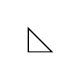
\begin{tikzpicture}[scale=0.3] \draw (0,0) -- (1,-1) -- (0,-1) --cycle; \end{tikzpicture}, note that given $g_1 \mapsto g$, every $\tau \in \Gamma_F$ multiplies $(\det g_1)^{-1/2} g_1 \in \SL(2, \bar{F})$ by a sign $c(\tau)$, and $\tau \mapsto c(\tau)$ represents the image of $g$ in $H^1(F, \mu_2)$. But the same cocycle represents the image of $\det(g_1)$ in $F^\times/F^{\times 2} \rightiso H^1(F, \mu_2)$.
\end{proof}

\subsection{Stable conjugacy: reduction to \texorpdfstring{$\SL(2)$}{SL2}}\label{sec:stable-reduction}
Fix a maximal $F$-torus $T$ in $G := \Sp(W)$. The lattices $X := X^*\left( T_{\bar{F}} \right)$ and $Y := X_*\left( T_{\bar{F}} \right)$ are endowed with $\Gamma_F$-actions. We choose an isomorphism $T_{\bar{F}} \simeq \Gm^n$ as in \S\ref{sec:Sp}, and enumerate the long roots (resp. short coroots) as $\pm 2\epsilon_1, \ldots, \pm 2\epsilon_n$ (resp. $\pm \check{\epsilon}_1, \ldots, \pm \check{\epsilon}_n$). Then $\Gamma_F$ acts on both sets and commutes with the bijection between roots and coroots. If $\mathcal{O}$ is a $\Gamma_F$-orbit, so is $-\mathcal{O}$. Now recall some definitions from \cite[\S 2]{LS1}.

\begin{definition}\label{def:symmetric-orbits}
	Let $\mathcal{O}$ be a $\Gamma_F$-orbit of roots.
	\begin{compactenum}[(i)]
		\item If $\mathcal{O}=-\mathcal{O}$, we say $\mathcal{O}$ is \emph{symmetric}.\index{symmetric root}
		\item If $\mathcal{O} \cap (-\mathcal{O}) = \emptyset$, we say $\mathcal{O}$ is \emph{asymmetric}.
	\end{compactenum}
	The same terminology pertains to $\Gamma_F$-orbits of coroots.
\end{definition}
For any root $\alpha$, set
\begin{equation}\label{eqn:F_alpha}\begin{gathered}
	\Gamma_\alpha := \Stab_{\Gamma_F}(\alpha) \subset \Stab_{\Gamma_F}(\{\pm\alpha\}) =: \Gamma_{\pm\alpha}, \\
	F_\alpha \supset F_{\pm\alpha} \supset F: \quad \text{their fixed fields in}\; \bar{F}.
\end{gathered}\end{equation}\index{F_\alpha@$F_{\alpha}, F_{\pm\alpha}$}
These extensions are all separable since the splitting field of $T$ is.

\begin{lemma}\label{prop:anisotropic-criterion}
	The torus $T$ is anisotropic if and only if every orbit $\mathcal{O}$ of long roots (resp. short coroots) is symmetric.
\end{lemma}
\begin{proof}
	For any orbit $\mathcal{O}$ of long roots, $\sum_{\alpha \in \mathcal{O}} \alpha \in X^{\Gamma_F} = 0$ if and only if $\mathcal{O}$ is symmetric. The existence of asymmetric $\mathcal{O}$ implies $X^{\Gamma_F} \neq 0$, thus $T$ is isotropic. Conversely, assume every $\mathcal{O}$ is symmetric and consider $v = \sum_{i=1}^n a_i\epsilon_i \in X^{\Gamma_F} \smallsetminus \{0\}$. For each $i$, there exists $\sigma \in \Gamma_F$ such that $\sigma(\pm\epsilon_i) = \mp\epsilon_i$ since $2\epsilon_i$ belongs to a symmetric orbit; from $\sigma(v)=v$ we deduce $a_i=0$. This implies $v=0$ so $T$ is anisotropic.
\end{proof}

Hereafter we only consider the orbits of long roots or short coroots.

Select a $\Gamma_F$-orbit $\mathcal{O}$ in $X$ together with a long $\alpha \in \mathcal{O}$. After base-change to $F_{\pm\alpha}$, we see that $\{\alpha,-\alpha\}$ generates a copy of $\SL(2)$ in $G_{F_{\pm\alpha}}$. This $\SL(2)$ contains the subtorus $T_{\pm\alpha}$ of $T_{\bar{F}}$ with $X_*(T_{\pm\alpha, \bar{F}}) = \Z\check{\alpha} \subset Y$; as a shorthand, we say $T_{\pm\alpha}$ is generated by $\alpha$. Hence $T_{\pm\alpha}$, $\SL(2)$ are both defined over $F_{\pm\alpha}$.

\begin{enumerate}
	\item First assume $\mathcal{O}$ is symmetric so that $(\Gamma_{\pm\alpha} : \Gamma_\alpha) = [F_\alpha : F_{\pm\alpha}] = 2$. In this case $T_{\pm\alpha}$ is anisotropic and it splits over $F_\alpha$, and
	\[ T_{\pm\alpha} \simeq F_\alpha^1 := \Ker \left[N_{F_\alpha/F_{\pm\alpha}}: F_\alpha^\times \to F_{\pm\alpha}^\times \right]. \]
	\item Next, assume $\mathcal{O}$ is asymmetric. Then $\Gamma_{\pm\alpha}=\Gamma_\alpha$, $F_\alpha = F_{\pm\alpha}$, and $T_{\pm\alpha}$ is a split.
\end{enumerate}
Identify $\mathcal{O}$ with $\Hom_F(F_\alpha, \bar{F}) = \Gamma_F/\Gamma_{F_\alpha}$. Let $T_{\mathcal{O}}$ be the subtorus of $T_{\bar{F}}$ generated by $\mathcal{O}$ in the sense above, which is now defined over $F$. By the generalities on reductive groups and their Weil restrictions (cf. \eqref{eqn:tensor-split}), we see that there is an embedding (see \S\ref{sec:Sp-parameters} for discussions on $\SL(2)$):
\begin{equation}\label{eqn:O-embedding-1} \begin{tikzcd}[baseline]
	-1 \in \SL(2, F_{\pm\alpha}) & R_{F_{\pm\alpha}/F}(\SL(2)) \arrow[hookrightarrow]{r} & G \\
	& R_{F_{\pm\alpha}/F}(T_{\pm\alpha}) \arrow[hookrightarrow]{u}{\text{max. torus}} & \\
	\quoted{-1} := \prod_{\pm \beta \in \mathcal{O}} \check{\beta}(-1) \arrow[mapsto]{uu} & T_{\mathcal{O}} \arrow[hookrightarrow]{r} \arrow{u}{\simeq} & T \arrow[hookrightarrow]{uu}[swap]{\text{max. torus}} \\
\end{tikzcd}\end{equation}
Denote the image of $R_{F_{\pm\alpha}/F}(\SL(2))$ as $G_{\mathcal{O}}$. It is a canonically defined subgroup of $G$ relative to $\mathcal{O}$. Observe that $(G_\mathcal{O}, T_\mathcal{O}) = (G_{-\mathcal{O}}, T_{-\mathcal{O}})$. Furthermore,
\[ \prod_{\pm\mathcal{O}} T_{\mathcal{O}} \rightiso T. \]

This construction can be described in terms of the parameter $(K, K^\sharp, c)$ of $T \hookrightarrow G$ supplied by Proposition \ref{prop:parameter-tori}. We shall use the familiar decomposition $K = \prod_{i \in I} K_i$.
\begin{itemize}
	\item When $T$ is split, we may assume $I = \{1, \ldots, n\}$, $K_i^\sharp = F$, and $K_i = F \times F$ for all $i$. Identify $T$ with $\left\{  (x_i, y_i)_{i=1}^n \in (F^\times \times F^\times)^n : x_i y_i = 1 \right\}$. Now $X = \bigoplus_{i=1}^n \Z\epsilon_i$ where $\epsilon_i$ (resp. $-\epsilon_i$) corresponds to $(x_i,y_i) \mapsto x_i$ (resp. $(x_i, y_i) \mapsto y_i$). The $\Gamma_F$-orbits of long roots are singletons $\{\pm 2\epsilon_i\}$; they are all asymmetric.
	\item The general case is obtained by a twist as follows. The set $I$ is in bijection with the sets $\{\mathcal{O}, -\mathcal{O}\}$ of $\Gamma_F$-orbits. We have $i \in I_0$ (i.e. $K_i$ is a field) if and only if $\pm\mathcal{O}$ are symmetric. By choosing an homomorphism $K_i \to \bar{F}$ of $F$-algebras, we pick out $\alpha \in \mathcal{O}$ and
	\begin{equation}\label{eqn:K_i-alpha} \begin{gathered}
		K_i^\sharp \simeq F_{\pm\alpha}; \qquad
		K_i \simeq \begin{cases} F_\alpha, & i \in I_0 \\ F_{\pm\alpha} \times F_{\pm\alpha}, & i \notin I_0. \end{cases}
	\end{gathered}\end{equation}
	Decompose $c = (c_i)_{i \in I}$ and define a symplectic form $h^i$ (resp. $h_i$) on the $K_i^\sharp$-vector space (resp. $F$-vector space) $K_i$ à la \eqref{eqn:K-symp-form} as
	\begin{equation}\label{eqn:h-h} \begin{aligned}
		h^i(u|v) & := \Tr_{K_i/K_i^\sharp} \left(\tau(u)v c_i \right), \\
		h_i(u|v) & := \Tr_{K_i/F} \left( \tau(u)v c_i \right) = \Tr_{K_i^\sharp/F} \left( h^i(u|v) \right).
	\end{aligned}\end{equation}
	Under this correspondence, \eqref{eqn:O-embedding-1} coincides with
	\begin{equation}\label{eqn:O-embedding-2} \begin{tikzcd}
		-1 \in \SL(2,K_i^\sharp) & G_{\mathcal{O}} = R_{K_i^\sharp/F}( \overbracket{\Sp(K_i, h^i)}^{= \SL(2)} ) \arrow[hookrightarrow]{r} & \Sp(K_i, h_i) \arrow[hookrightarrow]{r} & \Sp(W) = G \\
		-1 \in K_i^1 \arrow[mapsto]{u} & T_{\mathcal{O}} = K_i^1 \arrow[hookrightarrow]{rr} \arrow[hookrightarrow]{u} & & K^1 = T \arrow[hookrightarrow]{u}
	\end{tikzcd}\end{equation}
	\item The isomorphism $(W, \lrangle{\cdot|\cdot}) \simeq \bigoplus_{i \in I} (K_i, h_i)$ of symplectic $F$-vector spaces gives rise to
	\begin{gather*}
		\prod_{\pm \mathcal{O}} G_{\mathcal{O}} \simeq \prod_{i \in I} R_{K_i^\sharp/F}( \overbracket{\Sp(K_i, h^i)}^{=\SL(2)} ) \subset \prod_{i \in I} \Sp(K_i, h_i) \hookrightarrow \Sp(W) = G, \\
		\prod_{\pm \mathcal{O}} T_{\mathcal{O}} \simeq \prod_{i \in I} R_{K_i^\sharp/F}(K_i^1) = K^1 \simeq T. 
	\end{gather*}
\end{itemize}

\begin{definition}\label{def:G-T}
	Given $T$ as above, we set $G^T := \prod_{\pm\mathcal{O}} G_{\mathcal{O}}$. It is a canonically defined subgroup of $G$ containing $T$, and can be described as $\prod_{i \in I} R_{K_i^\sharp/F}(\SL(2))$ in terms of the parameter $(K, K^\sharp, c)$ for $T \hookrightarrow G$. \index{GT@$G^T$}
\end{definition}

By Shapiro's lemma, $H^1(F, G^T) = \prod_{i \in I} H^1(K_i^\sharp, \SL(2))$ is trivial. By the discussions in \S\ref{sec:Weil-restriction} on Weil restrictions, we see
\begin{compactitem}
	\item $G^T$ is simply connected since $\SL(2)$ is;
	\item $G^T_\text{ad} = \prod_{\pm \mathcal{O}} R_{F_{\pm\alpha}/F}(\PGL(2))$ since Weil restriction commutes with the formation of adjoint groups, as noted in \S\ref{sec:Weil-restriction};
	\item if $\Ad(g): T \rightiso T'$ is a stable conjugation inside $G^T$, then we have $G^T = G^{T'}$. In fact one can take $g \in G^T_\text{ad}(F)$ by Proposition \ref{prop:st-conj-SL2}.
\end{compactitem}

\begin{proposition}\label{prop:stable-reduction-SL2}
	Conserve the notations above and suppose $\delta \in T_\mathrm{reg}(F)$. Then every conjugacy class in the stable conjugacy class of $\delta$ contains an element of the form $g\delta g^{-1}$ where $g \in G^T_{\mathrm{ad}}(F)$, and
	\[ \mathrm{inv}(\delta, g\delta g^{-1}) = \text{image of $g$ under }\; G^T_{\mathrm{ad}}(F) \to \mathfrak{D}(Z_{G^T}, G^T; F) \to \mathfrak{D}(T, G; F). \]
	Furthermore, $\mathfrak{D}(Z_{G^T}, G^T; F) \to \mathfrak{D}(T, G; F)$ is bijective and in terms of parameters, $\mathrm{inv}(x, g\delta g^{-1})$ can be identified with
	\[ \left(\det(g_{i,1}) N_{K_i/K_i^\sharp}(K_i^\sharp) \right)_{i \in I} \; \in K^{\sharp,\times}/N_{K/K^\sharp}(K^\times). \]
	Here $g_{i,1} \in \GL(2, K_i^\sharp)$ is any representative of $g_i \in \PGL(2, K_i^\sharp)$.
\end{proposition}
Note that the indexes $i \notin I_0$ have no contribution, and $I=I_0$ when $T$ is anisotropic by Lemma \ref{prop:parameter-ani}.
\begin{proof}
	The first equality for $\text{inv}(\delta, g\delta g^{-1})$ reduces essentially to Proposition \ref{prop:adjoint-rel-pos}. The next step is to describe the image of $g$ in terms of $(g_{i,1})_{i \in I}$. The map $\mathfrak{D}(Z_{G^T}, G^T; F) \to \mathfrak{D}(T, G; F)$ factors into $\mathfrak{D}(Z_{G^T}, G^T; F) \to \mathfrak{D}(T, G^T; F) \to \mathfrak{D}(T, G; F)$, whilst $\mathfrak{D}(T, G^T; F) = H^1(F, T) = \mathfrak{D}(T, G; F)$. Proposition \ref{prop:D-description} asserts that
	\[ H^1(F,T) \simeq \prod_{i \in I} \dfrac{K_i^{\sharp,\times}}{N_{K_i/K_i^\sharp}(K_i^\times)} = \dfrac{K^{\sharp, \times}}{N_{K/K^\sharp}(K^\times)}. \]
	This is compatible with the decomposition $T = \prod_{i \in I} R_{K^\sharp_i/F}(K_i^1)$, so we may work separately for each $i \in I$. Shapiro's lemma affords the commutative diagram
	\[\begin{tikzcd}
		(R_{K_i^\sharp/F} \PGL(2))(F) \arrow[-, double equal sign distance]{d} \arrow{r} & H^1(F, R_{K_i^\sharp/F}(K^1)) \arrow{d}{\simeq} & \\
		\PGL(2, K_i^\sharp) \arrow{r} & H^1(K_i^\sharp, K^1) \arrow{r}{\simeq} & K_i^\sharp/N_{K_i/K_i^\sharp}(K^\times).
	\end{tikzcd}\]
	We are now reduced to the rank-one case of Proposition \ref{prop:st-conj-SL2} and the description of $\text{inv}(\delta, g\delta g^{-1})$ follows. Finally, this description implies the surjectivity of $G^T_\text{ad}(F) \to \mathfrak{D}(T,G;F)$, therefore every $\eta \stackrel{\text{st}}{\sim} \delta$ is conjugate to some $g\delta g^{-1}$ with $g \in G^T_\text{ad}(F)$.
\end{proof}

Summarizing, we obtain all stable conjugates of elements in $T_\text{reg} \subset G$ (up to ordinary conjugacy) by working inside $G^T$. Modulo Weil restrictions, the description of stable conjugacy boils down to the $\SL(2)$ case. There is also an obvious version for $\mathfrak{g}$.

\section{BD-covers of symplectic groups}\label{sec:BD-covers-Sp}
Except in \S\ref{sec:nr-global}, the assumptions in \S\ref{sec:Sp-gen} on the field $F$ remain in force. For the study of harmonic analysis, we can and do confine ourselves to the BD-covers of $\Sp(2n)$ arising from Matsumoto's central extension; see the Remarks \ref{rem:Matsumoto} and \ref{rem:rescaling-Q}.

\subsection{The covers}\label{sec:BD-Sp}
Let $(W, \lrangle{\cdot | \cdot})$ be a symplectic $F$-vector space of dimension $2n$. Fix a maximal $F$-torus $T$ of $G := \Sp(W)$ and set $Y = X_*(T_{\bar{F}})$. Write $G := \Sp(W)$ and denote by $E_G \to G$ the multiplicative $\shK_2$-torsor constructed by Matsumoto (Remark \ref{rem:Matsumoto}). It corresponds to the quadratic form $Q: Y \to \Z$ in \eqref{eqn:Y-Sp}. We will also write $E_{G,F}$ when the base field is to be stressed. When $\dim W = 2$ with chosen symplectic basis, we adopt the shorthand $E_G = E_{\SL(2)}$.

%\begin{remark}\label{rem:symplectic-transport}
%	Let $\varphi: (W, \lrangle{\cdot|\cdot}) \rightiso (W', \lrangle{\cdot|\cdot}')$ be an isomorphism of symplectic $F$-vector spaces, then $\Sp(W) \rightiso \Sp(W')$ is covered by a unique isomorphism $E_{\Sp(W)} \rightiso E_{\Sp(W')}$. Indeed, the form $Q: Y \to \Z$ transports to a Weyl and Galois-invariant quadratic form $Y' \to \Z$, which still takes value $1$ on short coroots, whence the existence of $E_{\Sp(W)} \rightiso E_{\Sp(W')}$. Since $G$ is simply connected, the uniqueness follows.
%\end{remark}

To $Q$ is associated the symmetric bilinear form on $Y$
\[ B_Q(y, y') := Q(y+y')-Q(y)-Q(y') = 2 \sum_{i=1}^n y_i y'_i. \]
Suppose $m \mid N_F$ as in \S\ref{sec:isogeny}. Since $Y_{Q,m} = \dfrac{m}{\text{gcd}(2,m)} Y \subset Y$, the isogeny $\iota_{Q,m}: T_{Q,m} \to T$, together with its compatibility under $G$-conjugation, can be identified with the endomorphism of $T \subset G$
\begin{equation}\label{eqn:isogeny-Sp} \begin{aligned}
	\iota_{Q,m}: T_{Q,m} = T & \longrightarrow T \\
	t & \longmapsto t^{m/\text{gcd}(2,m)}
\end{aligned}\end{equation}
\textbf{Caveat}: one must be careful when identifying $T_{Q,m}$ and $T$, as they will play different roles in our latter applications.

\begin{lemma}\label{prop:restriction-W_i}
	Suppose that $(W, \lrangle{\cdot|\cdot})$ is the orthogonal direct sum $\bigoplus_{i=1}^r W_i$ of symplectic vector subspaces. Write $G_i := \Sp(W_i) \hookrightarrow G$. There is a natural morphism $\iota_i: E_{G_i} \rightiso E_G|_{G_i}$ for all $1 \leq i \leq r$. They realize the pull-back of $E_G \to G$ to $G_1 \times \cdots \times G_r$ as the contracted product of multiplicative $\shK_2$-torsors $E_{G_1} \utimes{\shK_2} \cdots \utimes{\shK_2} E_{G_r}$.
	
	In particular, elements lying over different components $G_i$ commute in $E_G$.
\end{lemma}
\begin{proof}
	Choose symplectic bases of $W_1, \ldots, W_r$; their union is a symplectic basis of $W$. The corresponding split maximal $F$-torus of $G$ is $T = T_1 \times \cdots \times T_r$; in parallel $(Y, Q) = (Y_1, Q_1) \oplus \cdots \oplus (Y_r, Q_r)$ where $Q_i$ is the quadratic form associated to Matsumoto's $E_{G_i}$, by \eqref{eqn:Y-Sp}.

	By Remark \ref{rem:shared-torus}, $E_G|_{G_1 \times \cdots \times G_r}$ is also classified by the quadratic form $(Y, Q)$. On the other hand, $\bigoplus_{i=1}^r (Y_i, Q_i)$ corresponds to $E_{G_1} \utimes{\shK_2} \cdots \utimes{\shK_2} E_{G_r}$. This gives the required isomorphism. The required $\iota_i$ comes from composing with $E_{G_i} \hookrightarrow E_{G_1} \utimes{\shK_2} \cdots \utimes{\shK_2} E_{G_r}$.
\end{proof}

Now consider the constructions in \S\ref{sec:stable-reduction}. We have a maximal $F$-torus $T \subset G$. Form the canonical subgroup $T \subset G^T \subset G$ of Definition \ref{def:G-T}. By choosing a parameter $(K, K^\sharp, \ldots)$ for $T \hookrightarrow G$ (Proposition \ref{prop:parameter-tori}), we may identify $G^T$ with $\prod_{i \in I} R_{K^\sharp_i/F} \SL(2)$. To reconcile with the notations in \S\ref{sec:Weil-restriction}, denote by $f_i: \Spec(K_i^\sharp) \to \Spec(F)$ the structure morphisms for each $i \in I$.

\begin{theorem}\label{prop:G-T-reduction-K_2}
	The restriction of $E_G$ to $G^T$ is isomorphic to the contracted product of the multiplicative $\shK_2$-torsors $f_{i,*} \left( E_{\SL(2), K_i^\sharp} \right)$.\index{contracted product}
\end{theorem}
\begin{proof}
	Using the notation from \S\ref{sec:stable-reduction}, we restrict $E_G$ in stages
	\[ G^T = \prod_{i \in I} R_{K^\sharp_i/F} \Sp(K_i, h^i) \hookrightarrow \prod_{i \in I} \Sp(K_i, h_i) \hookrightarrow \Sp(W) = G. \]
	With $G_i := \Sp(K_i, h_i)$, Lemma \ref{prop:restriction-W_i} reduces the problem to the case $|I|=1$ and $K^\sharp$ is a field. Write $h = h^i$ and $f = f_i$. Since $R_{K^\sharp/F} \Sp(K, h)$ is simply connected and contains $T$, Remark \ref{rem:shared-torus} implies that $E_G|_{G^T}$ is classified by the $Q: Y \to \Z$ in \eqref{eqn:Y-Sp}.

	Now turn to the quadratic form $Q': Y \to \Z$ associated to $f_* E_{\Sp(K, h)}$. Choose a coroot $\check{\alpha}$ of $K^1 \subset \Sp(K,h)$, which is defined over $F_\alpha$ and recall $K^\sharp = F_{\pm\alpha}$ in the notation of \S\ref{sec:stable-reduction}. Then $Y_{\Sp(K,h)} = \Z\check{\alpha}$ and the $Q_{\Sp(K,h)}$ associated to $E_{\Sp(K,h)}$ is simply $y\check{\alpha} \mapsto y^2$ by \eqref{eqn:Y-Sp}. If $K$ is a field then $K=F_\alpha$ and $\Gal{F_\alpha/F_{\pm\alpha}}$ acts on $Y_{\Sp(K,h)}$ by $\check{\alpha} \mapsto \pm\check{\alpha}$, thus stabilizes $Q_{\Sp(K,h)}$. If $K \simeq K^\sharp \times K^\sharp$ then $T$ splits over $F_{\pm\alpha}$. By the discussions in \S\ref{sec:stable-reduction}, the $\{\iota(\check{\alpha}) : \iota \in \Gamma_F \}$ is precisely the set of short coroots in $Y$ respect to $T \subset G$ (over $\bar{F}$), therefore
	\begin{equation}\label{eqn:SL2-Y-restricted}
		Y = \bigoplus_{\iota \in \Gamma_F/\Gamma_{\pm\alpha}} \Z\iota(\check{\alpha}).
	\end{equation}
	This coincides with the description $\bigoplus_{\iota \in \Hom_F(K^\sharp, \bar{F})} Y_\iota$ of $f_* Y_{\Sp(K,h)}$ in \S\ref{sec:Weil-restriction}. Theorem \ref{prop:BD-restriction} gives the $Q'$ associated to $f_* E_{\Sp(K, h)}$: it is orthogonal direct sum of the forms
	\[ \Z\iota(\check{\alpha}) \to \Z, \quad y\iota(\check{\alpha}) \mapsto y^2, \quad (\iota \in \Gamma_F/\Gamma_{\pm\alpha}). \]
	By \eqref{eqn:SL2-Y-restricted} together with \eqref{eqn:Y-Sp}, we see $Q' = Q$. Therefore $f_* E_{\Sp(K,h)} \simeq E_G|_{G^T}$ in $\cate{CExt}(G^T, \shK_2)$.
\end{proof}

Let $m \mid N_F$. By the construction of \S\ref{sec:local-BD}, to $(E_G, m)$ is attached the topological central extension of locally compact groups
\begin{equation}\label{eqn:G-BD-cext}
	1 \to \mu_m \to \tilde{G} \xrightarrow{\bm{p}} G(F) \to 1.
\end{equation}
When $G = \SL(2,F)$, denote by $\widetilde{\SL}(2, F)$ the topological central extension of $\SL(2,F)$ by $\mu_m$ so obtained.

\begin{theorem}\label{prop:G-T-reduction}
	The restriction of $\tilde{G}$ to $G^T(F)$ is isomorphic to the contracted product of the topological central extensions $\widetilde{\SL}(2, K_i^\sharp)$ by $\mu_m$.
\end{theorem}
When $K_i^\sharp = \CC$, we set $\widetilde{\SL}(2, K_i^\sharp) := \SL(2,\CC) \times \mu_m$, so that the assertion always makes sense.
\begin{proof}
	Consider the push-out to $\mu_m$ of the contracted product of $\left( f_{i,*} E_{\SL(2), K_i^\sharp} \right)(F)$; it is canonically isomorphic to the contracted product of the push-outs of $\left( f_{i,*} E_{\SL(2), K_i^\sharp} \right)(F)$ to $\mu_m$. The latter push-outs are isomorphic to $\widetilde{\SL}(2, K_i^\sharp)$ as topological central extensions of $\SL(2, K_i^\sharp)$ by $\mu_m$, by Proposition \ref{prop:BD-restriction}. We conclude by applying Theorem \ref{prop:G-T-reduction-K_2}.
\end{proof}


\subsection{Kubota's cover of \texorpdfstring{$\GL(2)$}{GL2}}\label{sec:Kubota}
We review Kubota's description \cite{Ku69} of a covering of $\GL(2,F)$, cf. \cite[0.1]{KP84} and \cite[\S 16.2]{GG}. It is a multiplicative $\shK_2$-torsor $E_\text{Ku} \to \GL(2)$ such that
\begin{compactitem}
	\item $E_\text{Ku}$ restricts to Matsumoto's $E_{\SL(2)} \to \SL(2)$, see \cite[0.1]{KP84};
	\item by \cite[p.41]{KP84}, there is a preferred section $\bm{s}: \GL(2,F) \to E_\text{Ku}(F)$ with $\bm{s}(x)\bm{s}(y) = \bm{c}(x,y) \bm{s}(xy)$ in terms of an explicit $2$-cocycle $\bm{c}$.
\end{compactitem} \index{xbold@$\bm{x}(\cdot), \bm{s}, \bm{c}$}
Using the notations of \S\ref{sec:local-BD}, we describe $\bm{c}$ by
\begin{equation}\label{eqn:Kubota-cocycle}
	\begin{gathered}
		\bm{x}\twobigmatrix{a}{b}{c}{d} := \begin{cases}
		c, & c \neq 0 \\
		d, & c = 0,
	\end{cases} \\
	\bm{c}(g_1, g_2) := - \left\{ \dfrac{ \bm{x}(g_1) }{ \bm{x}(g_1 g_2) }, \; \dfrac{ \det g_1 \cdot \bm{x}(g_2) }{ \bm{x}(g_1 g_2) } \right\}_F \; \in K_2(F).
\end{gathered}\end{equation}

\begin{remark}\label{rem:Kubota-minus}
	We follow \cite[Corollaire 5.12]{Mat69} to take the negative of the usual Kubota's cocycle found in \cite{Ku69, Fl80, KP84}, otherwise $E_{\text{Ku}}|_{\SL(2)}$ would be the negative of Matsumoto's central extension. For the relation between $\bm{s}$ and Steinberg's presentation for $E_{\SL(2)}(F)$, we refer to the discussions preceding \cite[Corollaire 5.12]{Mat69}. After pushing-out to $\mu_2$, the difference disappears.
\end{remark}
% see also \cite[\S 2.1]{BF15} for this minus sign

\begin{lemma}\label{prop:PGL-action}
	The adjoint action of $\GL(2)$ on $E_{\mathrm{Ku}}$ induces the canonical $\PGL(2)$-action on $E_{\SL(2)}$ given by Proposition \ref{prop:BD-adjoint-action}.
\end{lemma}
\begin{proof}
	The $\GL(2)$-action leaves $\SL(2)$ and $E_{\text{Ku}}|_{\SL(2)} = E_{\SL(2)}$ invariant. The center of $\GL(2)$ acts trivially on $\SL(2)$, thereby giving rise to an automorphism of $E_{\SL(2)} \to \SL(2)$; this action must be trivial as $\SL(2)$ is simply connected. We conclude by the uniqueness part of Proposition \ref{prop:BD-adjoint-action}.
\end{proof}

\begin{lemma}\label{prop:-1-adjoint}
	Let $g \in \PGL(2,F)$ with preimage $g_1 \in \GL(2,F)$. For any preimage $\widetilde{-1} \in E_{\mathrm{Ku}}(F)$ of $-1$, we have $\Ad(g)(\widetilde{-1}) = g_1 (\widetilde{-1}) g_1^{-1} = \xi (\widetilde{-1})$ where
	\[ \xi = -\left\{ -1, \det g_1 \right\}_F \in K_2(F). \]
\end{lemma}
\begin{proof}
	By Lemma \ref{prop:PGL-action} we have $\Ad(g)(\widetilde{-1}) = g_1(\widetilde{-1})g_1^{-1}$. As $-1$ is central in $\GL(2,F)$, we have $\xi = \bm{c}(g_1, -1) - \bm{c}(-1, g_1)$. Write $g_1 = \twomatrix{a}{b}{c}{d}$. First suppose $c \neq 0$, then $\bm{c}(g_1, -1) = -\left\{ -1, (\det g_1) c^{-1} \right\}_F$ whereas $\bm{c}(-1, g_1) = -\left\{ c^{-1}, -1 \right\}_F = -\left\{ -1, c^{-1} \right\}_F$ by the anti-symmetry of Steinberg symbols. Hence $\bm{c}(g_1, -1) - \bm{c}(-1, g_1) = -\left\{ -1, \det g_1 \right\}_F$.
	
	If $c = 0$, replacing $c$ by $d$ in the arguments above gives the same result.
\end{proof}

By fixing $m \mid N_F$ and pushing $E_\text{Ku}(F)$ out via $(\cdot, \cdot)_{F,m}: K_2(F) \to \mu_m$, we obtain a topological central extension
\[ 1 \to \mu_m \to \widetilde{\GL}(2,F) \to \GL(2,F) \to 1. \]
The resulting preferred section and cocycle are still denoted by $\mathbf{s}$ and $\bm{c}$, now with $\{\cdot, \cdot \}_F$ replaced by $(\cdot, \cdot)_{F,m}$. Hence
\begin{compactitem}
	\item $\widetilde{\GL}(2,F)$ restricts to $\widetilde{\SL}(2,F) \to \SL(2,F)$;
	\item by Lemma \ref{prop:PGL-action}, the adjoint action of $\GL(2,F)$ on $\widetilde{\SL}(2,F)$ induces the canonical $\PGL(2,F)$-action on $\widetilde{\SL}(2,F)$ from Proposition \ref{prop:BD-adjoint-action};
	\item the statements in Lemma \ref{prop:-1-adjoint} hold for $\widetilde{\SL}(2,F)$, with $\{\cdot,\cdot\}_F$ replaced by $( \cdot, \cdot)_{F,m}$.
\end{compactitem}

Let $K$ be an étale $F$-algebra of dimension $2$, therefore comes equipped with an involution $\tau \neq \identity$. The $F$-torus $K^\times$ embeds into $\GL(2)$ with $\det|_{K^\times} = N_{K/F}$; it restricts to $K^1 \hookrightarrow \SL(2)$. As the $n=1$ case of Proposition \ref{prop:D-description}, this parameterize stable conjugacy classes of embeddings of maximal tori in $\SL(2)$.

\begin{notation}
	When $K \simeq F \times F$, the elements are expressed as $x = (x_1, x_2)$ and we have $\tau(x_1, x_2) = (x_2, x_1)$. The Hilbert symbols for such $K$ can be conveniently defined as
	\[ (x,y)_{F,m} := (x_1, y_1)_{F,m} (x_2, y_2)_{F,m}. \]
\end{notation}

The result below quantifies the non-commutativity of the preimage of $K^\times$ in $\widetilde{\GL}(2,F)$.
\begin{proposition}[Flicker]\label{prop:Flicker-comm}
	Suppose that $\gamma, g \in \GL(2,F)$ arise from $x, u \in K^\times$. Let $\tilde{\gamma}$ be any preimage of $\gamma$ in $\widetilde{\GL}(2,F)$. The factor $[g,\gamma] \in \mu_m$ in \eqref{eqn:commutator} determined by $g\tilde{\gamma}g^{-1} = [g, \gamma] \tilde{\gamma}$ has the form
	\[ [g,\gamma] = (x, \tau(u))_{K,m}^{-1}. \]
\end{proposition}
\begin{proof}
	This is done in the calculations in \cite[p.128]{Fl80} using the cocycle $-\bm{c}$.
\end{proof}

In the situation above, we define
\begin{align*}
	\iota_{Q,m}: K^1 & \longrightarrow K^1 \\
	x_0 & \longmapsto x_0^{m/\mathrm{gcd}(2,m)}
\end{align*}
following \eqref{eqn:isogeny-Sp}. Given $x = \iota_{Q,m}(x_0)$, there exists $\omega \in K^\times$ with $\omega/\tau(\omega) = x_0$ by Hilbert's theorem 90. Then $N_{K/F}(\omega)$ is well-defined modulo $F^{\times 2}$. When $K \simeq F \times F$ and $x_0 = (a, a^{-1})$ with $a \in F^\times$, we may take $\omega = (a,1)$ to see that $N_{K/F}(\omega)$ represents the class of $a$ inside $F^\times/F^{\times 2}$.

We will need the \emph{projection formula} for the next proof
\begin{equation}\label{eqn:Hilbert-projection-formula}
	(a, b)_{K,m} = (a, N_{K/F}(b))_{F,m}, \quad a \in F^\times, \; b \in K^\times;
\end{equation}
it is standard when $K$ is a field, and the case $K \simeq F \times F$ is straightforward.

\begin{lemma}\label{prop:commutator-GL2-T}
	Suppose $x = \iota_{Q,m}(x_0) \in K^1$ and choose $\omega$ be as above. Then in the setting of Proposition \ref{prop:Flicker-comm} we have
	\begin{align*}
		[g,\gamma] & = \left( \omega, N_{K/F}(u) \right)_{K, \mathrm{gcd}(2,m)} = \left( \omega, \det\gamma \right)_{K, \mathrm{gcd}(2,m)} \\
		& = \left( N_{K/F}(\omega), \det\gamma \right)_{F, \mathrm{gcd}(2,m)}.
	\end{align*}
\end{lemma}
In particular, in this case $[g,\gamma]=1$ whenever $m \notin 2\Z$. It also follows that $\left( N_{K/F}(\omega), \det\gamma \right)_{F, \mathrm{gcd}(2,m)}$ is independent of the choice of $\omega$, although this can also be verified directly.
\begin{proof}
	From \eqref{eqn:norm-residue-d} and the Proposition \ref{prop:Flicker-comm} we infer
	\begin{align*}
		[g, \gamma] & = \left( x_0^{m/\text{gcd}(2,m)}, \tau(u) \right)_{K,m}^{-1} = \left( x_0, \tau(u) \right)_{K, \text{gcd}(2,m)} \\
		& = \left( \omega, \tau(u)\right)_{K, \text{gcd}(2,m)} \left( \tau(\omega)^{-1}, \tau(u) \right)_{K, \text{gcd}(2,m)} \\
		& = \left( \omega, \tau(u)\right)_{K, \text{gcd}(2,m)} \left( \omega, u \right)_{K, \text{gcd}(2,m)} \\
		& = \left( \omega, N_{K/F}(u) \right)_{K, \text{gcd}(2,m)} = \left( \omega, \det\gamma \right)_{K, \text{gcd}(2,m)}.
	\end{align*}
	Now apply \eqref{eqn:Hilbert-projection-formula} to obtain the remaining equality in the assertion.
\end{proof}

We will need further invariance properties for this factor.
\begin{definition-proposition}\label{def:Cali-factor}\index{Cm@$\Cali_m(\nu, \gamma_0)$}
	Take $x_0 = \omega/\tau(\omega) \in K^1$ as before, and let $\nu \in F^\times/F^{\times 2}$. Let $\gamma_0 \in \SL(2,F)$ be associated to $x_0$ via $K^1 \hookrightarrow \SL(2)$ and put
	\[ \Cali_m(\nu, \gamma_0) := \left( N_{K/F}(\omega), \nu \right)_{F, \mathrm{gcd}(2,m)}. \]
	Then $\Cali_m(\nu, \gamma_0)$ depends only on the stable conjugacy class of the element $\gamma_0 \in \SL(2,F)$ associated to $x$. Furthermore, $\Cali_m(\nu, \gamma_0)$ is invariant under any automorphism of the $F$-group $\SL(2)$.
\end{definition-proposition}
\begin{proof}
	Given a stable conjugacy class $\gamma_0$, the datum $(K, x_0)$ is determined up to isomorphisms of étale $F$-algebras, thus $N_{K/F}(\omega)$ is determined up to $F^{\times 2}$. Hence $\Cali_m(\nu, \gamma_0)$ is invariant under $\PGL(2,F)$, and $\PGL(2)$ equals the $F$-scheme of automorphisms of $\SL(2)$ by \cite[Exp XXIV, Théorème 1.3]{SGA3-3}.
\end{proof}

Observe that $\Cali_m(\nu, \gamma_0)$ is bi-multiplicative in $\nu$ and $\gamma_0$. In applications, $\nu$ will arise from the $\nu(g)$ in \eqref{eqn:nu-arises}.

We record the classification by K.\! Hiraga and T.\! Ikeda of good regular semisimple elements in $\widetilde{\SL}(2,F)$. Write $T \subset \SL(2)$ for the maximal $F$-torus parameterized by a two-dimensional étale $F$-algebra $K$.

\begin{theorem}[Hiraga--Ikeda]\label{prop:good-SL2} \index{good element}
	The projection of $Z_{\tilde{T}}$ to $T(F)$ equals $\{\pm 1\} \cdot T(F)^{m/\mathrm{gcd}(2,m)}$. In particular, $\gamma \in T_{\mathrm{reg}}(F)$ is good if and only if $\gamma \in \{\pm 1\} \cdot T(F)^{m/\mathrm{gcd}(2,m)}$.
\end{theorem}
\begin{proof}
	Their original proof is reproduced below. We begin by showing that the preimage of $\{\pm 1\} \cdot T(F)^{m/\mathrm{gcd}(2,m)}$ is central. In view of Proposition \ref{prop:good-in-tori} and \eqref{eqn:isogeny-Sp}, it suffices to show $[\pm 1, \eta] = 1$ for all $\eta \in \SL(2,F)$: this is already true on the $K_2(F)$-level by Proposition \ref{prop:BD-adjoint-action}.
	
	Now suppose $\gamma \in T(F)$ is projected from $Z_{\tilde{T}}$. Set $m_0 := m/\mathrm{gcd}(2,m)$. When $T$ is split, by Proposition \ref{prop:good-in-tori} we have $\gamma \in T(F)^{m_0}$. Thus we can assume $T$ is associated with a quadratic extension of fields $K$ of $F$, and $\gamma$ corresponds to $x \in K^1$. Proposition \ref{prop:Flicker-comm} implies that for all $v \in K^\times$,
	\begin{align*}
		1 & = \left( x, \tau(v)/v \right)_{K,m} \\
		& = ( x, \tau(v) )_{K,m} ( x, v^{-1})_{K,m} = ( \tau(x), v )_{K,m} ( x, v^{-1} )_{K,m} \\
		& = ( x^{-1}, v )_{K,m} ( x, v^{-1} )_{K,m} = \left( x^2, v^{-1} \right)_{K, m}.
	\end{align*}
	This shows $\pm x \in K^1 \cap K^{\times m_0}$ and it remains to show $K^1 \cap K^{\times m_0} = \pm (K^1)^{m_0}$.
	
	We have $-1 \in K^{\times m_0}$, because $(-1)^{m_0} = -1$ when $4 \nmid m$ whilst $\zeta^{m_0} = -1$ when $4 \mid m$ and $\mu_m = \lrangle{\zeta}$. Therefore $K^1 \cap K^{\times m_0} \supset \pm (K^1)^{m_0}$. Next, suppose $y_0 \in K^\times$ satisfies $N_{K/F}(y_0^{m_0}) = 1$, then there exists $\xi \in \mu_m$, $\xi^{m_0} = \pm 1$ such that $N_{K/F}(y_0) = \xi^2$. This leads to $y_1 := \xi^{-1} y_0 \in K^1$ satisfying $(y_1)^{m_0} = \xi^{-m_0} y_0^{m_0} = \pm y_0^{m_0}$; we conclude that $K^1 \cap K^{\times m_0} \subset \pm (K^1)^{m_0}$.
	
	The last assertion results from Corollary \ref{prop:isogeny-good}.
\end{proof}

Below is a supplement to the classification above.
\begin{proposition}\label{prop:iota-kernel}
	Let $T \simeq K^1$ as above, then
	\begin{align*}
		T(F)^{m/\mathrm{gcd}(2,m)} = (-1) \cdot T(F)^{m/\mathrm{gcd}(2,m)}, & \quad  4 \nmid m \quad \text{or}\quad T: \text{split}, \\
		T(F)^{m/\mathrm{gcd}(2,m)} \cap (-1) \cdot T(F)^{m/\mathrm{gcd}(2,m)} = \emptyset, & \quad 4 \mid m \quad\text{and}\quad T: \text{anisotropic}.
	\end{align*}
	On the other hand,
	\begin{equation}
		\Ker(\iota_{Q,m}) = \begin{cases}
			\mu_{m/\mathrm{gcd}(2,m)}, & T: \text{split} \\
			1, & 4 \nmid m, \quad T: \text{anisotropic} \\
			\{\pm 1 \}, & 4 \mid m, \quad T: \text{anisotropic};
	\end{cases}\end{equation}
	in the split case, $K \simeq F \times F$ and we embed $\mu_m$ into $K^1$ via $z \mapsto (z, z^{-1})$.
\end{proposition}
\begin{proof}
	For the first part, note that $(\pm 1) \cdot T(F)^{m/\text{gcd}(2,m)}$ are either identical or disjoint. They are identical if and only if $-1 = \xi^{m/\text{gcd}(2,m)}$ for some $\xi \in K^1$. When $4 \nmid m$, taking $\xi = -1$ suffices. When $T$ splits (so $K \simeq F \times F$) and $4 \mid m$, we may take $\xi = (\zeta, \zeta^{-1})$ where $\mu_m = \lrangle{\zeta}$, since $\zeta^{m/2} = -1$.

	When $4 \mid m$ and $T$ is anisotropic, we know $K$ is a field; by $\xi^m = 1$ and $m \mid N_F$ we obtain $\xi \in F^\times$. Moreover, $N_{K/F}(\xi)=1$ implies $\xi = \pm 1$, but $(-1)^{m/2} = 1$.

	For the second part, the case $K = F \times F$ is straightforward. When $K$ is a field, $\iota_{Q,m}(x_0) = 1 \implies x_0 \in F^\times \cap K^1$ since $m \mid N_F$, hence $x_0 = \pm 1$ as before; it remains to observe that $(-1)^{m/\text{gcd}(2,m)} = 1$ if and only if $4 \mid m$.
\end{proof}

\subsection{Stable conjugacy for BD-covers}\label{sec:st-conj-BD}
Revert to the notation of \S\ref{sec:Sp} and \S\ref{sec:BD-Sp}. Fix a maximal $F$-torus $T$. The subgroup $T \subset G^T \subset G$ (Definition \ref{def:G-T}) together with the decomposition $G^T = \prod_{\mathcal{O}/\pm} G_{\mathcal{O}}$ are canonically defined by $T$. Once a parameter $(K, K^\sharp, \ldots)$ for $T$ is chosen, $G^T$ together with its decomposition can be identified with $\prod_{i \in I} R_{K_i^\sharp/F}(\SL(2))$, and $T$ is identified with $\prod_{i \in I} R_{K_i^\sharp/F}(K_i^1)$.

Given $\delta \in T_\text{reg}(F)$ and $\eta \in G_\text{reg}(F)$, recall that $\mathcal{T}(\delta, \eta) := \{g: g\delta g^{-1} = \eta \}$ is nonempty if and only if $\delta \stackrel{\text{st}}{\sim} \eta$, in which case it is a right $T$-torsor. As a first step, we assume $\eta \in G^T(F)$ so that Proposition \ref{prop:stable-reduction-SL2} entails $\mathcal{T}(\delta, \eta) \subset G^T$. In parallel with the decomposition of $G^T$, we have $\mathcal{T}(\delta, \eta) = \prod_{i \in I} \mathcal{T}_i(\delta_i, \eta_i)$, where each $\mathcal{T}_i(\cdots)$ is defined inside $R_{K_i^\sharp/F} (\SL(2))$.

Now suppose $\eta \in G_\text{reg}(F)$ is stably conjugate to $\delta \in T_\text{reg}(F)$. Denote $S := G_\eta$. By Proposition \ref{prop:stable-reduction-SL2}, the canonical isomorphism of pointed tori $\Ad(g): (T, \delta) \rightiso (S, \eta)$ induced by any $g \in \mathcal{T}(\delta, \eta)(\bar{F})$ can be decomposed as
\[\begin{tikzcd}
	(T, \delta) \arrow{r}{\Ad(g')} \arrow[bend right]{rr}[swap]{\Ad(g)} & (T', \delta') \arrow{r}{\Ad(g'')} & (S, \eta)
\end{tikzcd}\]
for some $\delta' \in G^T_\text{reg}(F)$, $g' \in \mathcal{T}^{G^T}(\delta, \delta')(\bar{F})$ and $g'' \in \mathcal{T}(\delta', \eta)(F)$. In particular $\Ad(g')(\delta') = \eta$ is ordinary conjugacy and
\[ \text{inv}(\delta, \eta) = \text{inv}(\delta, \delta'). \]
This equality also determines $\delta'$ up to $G^T(F)$-conjugacy. The goal of this subsection is to adapt these to good elements in $\tilde{G}_\text{reg}$ for the BD-cover $
\tilde{G} \twoheadrightarrow G(F)$.

Fix $m \mid N_F$. Denote by $\widetilde{G^T}$ the pull-back of $\mu_m \hookrightarrow \tilde{G} \twoheadrightarrow G(F)$ to $G^T(F)$. Theorem \ref{prop:G-T-reduction} says that as topological central extensions $\widetilde{G^T}$ is isomorphic to the contracted product of $\mu_m \hookrightarrow \widetilde{\SL}(2, K_i^\sharp) \twoheadrightarrow \SL(2, K_i^\sharp)$. Here it is convenient to identify $\iota_{Q,m}$ with the endomorphism $t_0 \mapsto t_0^{m/\text{gcd}(2,m)}$ of $T$ by \eqref{eqn:isogeny-Sp}; this decomposes into $\iota_{Q_i, m}: K_i^1 \to K_i^1$ for each $i \in I$.

\begin{proposition}\label{prop:good-T}
	The projection of $Z_{\tilde{T}}$ to $T(F)$ equals
	\[ \prod_{i \in I} \{\pm 1 \} \cdot \Image\left( \iota_{Q_i,m} \right). \]
	In particular, its intersection with $T_\mathrm{reg}(F)$ equals the set of good elements in $T_\mathrm{reg}(F)$.
\end{proposition}
\begin{proof}
	By the decomposition of $\widetilde{G^T}$, we reduce immediately to the case $\tilde{G} = \widetilde{G^T} = \widetilde{\SL}(2, F)$ treated in Theorem \ref{prop:good-SL2}, upon passing to a finite extension of $F$.
\end{proof}

\begin{remark}\label{rem:good-pm1}
	Every element $\eta = (\gamma_i)_{i \in I} \in \prod_{i \in I} \{\pm 1\}$ is good with respect to $\tilde{G} \twoheadrightarrow G(F)$. Indeed, Lemma \ref{prop:restriction-W_i} reduces the problem to the case $\eta \in \{\pm 1\}$, and one concludes by Proposition \ref{prop:BD-adjoint-action}.
\end{remark}

\begin{notation}\index{TQm-tilde@$\tilde{T}_{Q,m}, \tilde{T}_{Q,m}^\sigma$}
	Recall that $I$ can be identified with $\{ \text{long roots} \} \big/ \lrangle{\Gamma_F, \pm}$, thus canonical for the given $T$. The embedding $\{\pm 1\}^I \hookrightarrow T(F)$ is also definable in terms of long roots by \eqref{eqn:O-embedding-1}, hence canonical and can be transported under stable conjugacy. Let $\{\pm 1\}^I$ act on $T$ by coordinate-wise multiplication. Consider $\sigma = (\sigma_i)_{i \in I} \in \{\pm 1\}^I$. Pull-back of $\bm{p}: \tilde{T} \twoheadrightarrow T(F)$ along $\sigma \cdot \iota_{Q,m}$ yields
	\begin{equation}\label{eqn:iota-cover}\begin{aligned}
		\tilde{T}^\sigma_{Q,m} & := \left\{ (\tilde{t}, t_0) \in \tilde{T} \times T_{Q,m}(F) : \bm{p}(\tilde{t}) = \sigma \cdot \iota_{Q,m}(t_0) \right\}, \\
		\tilde{T}_{Q,m} & := \tilde{T}^{(+, \ldots, +)}_{Q,m}.
	\end{aligned}\end{equation}
	There are natural maps $\tilde{T} \xleftarrow{\text{pr}_1} \tilde{T}^\sigma_{Q,m} \xrightarrow{\text{pr}_2} T_{Q,m}(F)$. Proposition \ref{prop:good-T} implies that every good regular element in $\tilde{G}_\text{reg}$ lies in some $\text{pr}_1\left(\tilde{T}^\sigma_{Q,m}\right)$; when $4 \nmid m$, it suffices to use $\sigma = (+, \ldots, +)$.
\end{notation}

Note that $\tilde{T}_{Q,m}$ is a group, whilst $\tilde{T}^\sigma_{Q,m}$ is only a $\tilde{T}_{Q,m}$-torsor for general $\sigma$.

Consider a stable conjugation $\Ad(g): T \rightiso S$ between maximal $F$-tori in $G$, then
\begin{itemize}
	\item as explicated above, $\{\pm 1\}^I \hookrightarrow T(F)$ can be transported to $S$ by $\Ad(g)$, thus $\tilde{S}^\sigma_{Q,m}$ makes sense;
	\item under the identification, $\sigma \cdot \Ad(g)(t) = \Ad(g)(\sigma \cdot t)$ for all $t \in T(F)$ and $\sigma \in \{\pm 1\}^I$; 
	\item if moreover $g \in G(F)$, from \eqref{eqn:isogeny-Ad} we have
	\begin{align*}
		\Ad(g): \tilde{T}^\sigma_{Q,m} & \longrightiso \tilde{S}^\sigma_{Q,m} \\
		(\tilde{t}, t_0) & \longmapsto (\Ad(g)(\tilde{t}), \Ad(g)(t_0))
	\end{align*}
	which is a group isomorphism for $\sigma = (+, \ldots, +)$, and is an equivariant map between torsors for general $\sigma$. Proposition \ref{prop:good-T} implies that $\Ad(g) = \identity$ when $g \in T(F)$.
\end{itemize}

Now comes the stable conjugacy in the $G \simeq \SL(2)$ case; the notation above reduces to $\tilde{T}^\pm_{Q,m}$. We will employ systematically the $G_\text{ad}(F)$-action on $\tilde{G}$ from Proposition \ref{prop:BD-adjoint-action}, again denoted by $\Ad$.

\begin{definition-proposition}\label{def:st-conj-SL2}\index{CAd@$\CaliAd$}
	Suppose that $\dim_F W = \dim_F K = 2$, so that $K^\sharp = F$ and $G^T = G$. Let $\Ad(g): T \rightiso S$ be a stable conjugation of maximal $F$-tori; here we may assume $g \in G_\mathrm{ad}(F)$ by Proposition \ref{prop:st-conj-SL2}. Set $\nu := \nu(g) \in F^\times/F^{\times 2}$ by \eqref{eqn:nu-arises}.
	\begin{enumerate}
		\item Define an isomorphism $\CaliAd(g) = \CaliAd^+(g): \tilde{T}^+_{Q,m} \to \tilde{S}^+_{Q,m}$ that fits into the commutative diagram
			\begin{equation*}\begin{gathered} \begin{tikzcd}[row sep=small]
				T(F) \arrow{r}{\Ad(g)} & S(F) \\
				\tilde{T}^+_{Q,m} \arrow{r}{\CaliAd^+(g)} \arrow{u} \arrow{d} & \tilde{S}^+_{Q,m} \arrow{u} \arrow{d} \\
				T_{Q,m}(F) \arrow{r}[swap]{\Ad(g)} \arrow[bend left=50]{uu}{\iota_{Q,m}} & S_{Q,m}(F) \arrow[bend right=50]{uu}[swap]{\iota_{Q,m}}
			\end{tikzcd} \\
				\CaliAd^+(g)(\tilde{t}, t_0) = \left( \Cali_m(\nu, t_0) \cdot \Ad(g)(\tilde{t}), \quad \Ad(g)(t_0) \right).
			\end{gathered}\end{equation*}
		\item When $4 \mid m$, define $\CaliAd^-(g): \tilde{T}^-_{Q,m} \to \tilde{S}^-_{Q,m}$ that fits into the commutative diagram
			\begin{equation*}\begin{gathered} \begin{tikzcd}[row sep=small]
				T(F) \arrow{r}{\Ad(g)} & S(F) \\
				\tilde{T}^-_{Q,m} \arrow{r}{\CaliAd^-(g)} \arrow{u} \arrow{d} & \tilde{S}_{Q,m} \arrow{u} \arrow{d} \\
				T_{Q,m}(F) \arrow{r}[swap]{\Ad(g)} \arrow[bend left=50]{uu}{(-1)\iota_{Q,m}} & S_{Q,m}(F) \arrow[bend right=50]{uu}[swap]{(-1)\iota_{Q,m}}
			\end{tikzcd} \\
				\CaliAd^-(g)\left( \widetilde{-1} \cdot \tilde{t}', t_0 \right) = \left( \Cali_m(\nu, t_0) \cdot \widetilde{-1} \cdot \Ad(g)(\tilde{t}'), \quad \Ad(g)(t_0) \right)
			\end{gathered}\end{equation*}
			for any $\widetilde{-1} \mapsto -1$ and $\tilde{t}' \mapsto \iota_{Q,m}(t_0)$.
	\end{enumerate}
	These constructions are independent of all choices. In particular it is independent of the identification $G \simeq \SL(2)$.
\end{definition-proposition}
\begin{proof}
	We may choose a preimage $g_1 \in \GL(2,F)$ of $g \in \PGL(2,F)$ by identifying $G$ and $\SL(2)$, and then apply the constructions in \S\ref{sec:Kubota}. By Definition--Proposition \ref{def:Cali-factor}, the factor $\Cali_m(\nu, t_0)$ depends only on $g \bmod \Image[G(F) \to G_\text{ad}(F)]$ and on the stable conjugacy class of $t_0$; it is invariant under any re-parameterization or automorphisms of $\SL(2)$.
\end{proof}

The following properties will also hold for stable conjugacy in general. We begin with the $\SL(2)$ case above.
\begin{proposition}\label{prop:CAd-prop}
	For any sign $\sigma$ that is allowed in our situation, the maps $\CaliAd^\sigma(g)$ satisfy the following properties.
	\begin{enumerate}[\bfseries{AD}.1.\;]
		\item $\CaliAd^\sigma(g)(\noyau\tilde{t}) = \noyau \CaliAd^\sigma(g)(\tilde{t})$ whenever $\noyau \in \mu_m$.
		\item $\CaliAd(g): \tilde{T}_{Q,m} \rightiso \tilde{S}_{Q,m}$ is an isomorphism of topological groups. In general, $\CaliAd^\sigma(g)$ is a $\CaliAd(g)$-equivariant map between torsors with respect to $\tilde{T}_{Q,m} \xrightarrow{\CaliAd(g)} \tilde{S}_{Q,m}$.
		\item If $g \in G(F)$, then $\CaliAd^\sigma(g)$ reduces to ordinary conjugation. If $g \in T(\bar{F})$, it equals $\identity$.
		\item Given stable conjugations of maximal $F$-tori $T \xrightarrow{\Ad(h)} S \xrightarrow{\Ad(g)} R$, we have
		\[ \CaliAd^\sigma(g) \circ \CaliAd^\sigma(h) = \CaliAd^\sigma(gh): \tilde{T}^\sigma_{Q,m} \to \tilde{R}^\sigma_{Q,m}. \]
	\end{enumerate}
\end{proposition}
\begin{proof}
	The setting under consideration is $G=\SL(2)$, $g,h \in G_\text{ad}(F)$.
	\begin{asparaenum}[\bfseries{AD}.1.\;]
	\item It follows from the analogous property of the $G_\text{ad}(F)$-action on $\tilde{G}$.
 
	\item Since $\Cali_m(\nu, t_0 t'_0) = \Cali_m(\nu, t_0) \Cali_m(\nu, t'_0)$ and $\Cali_m(\nu, \cdot)$ is locally constant, $\CaliAd(g)$ is a continuous homomorphism. It will follow from \textbf{AD.4} that $\CaliAd(g) \CaliAd(g^{-1}) = \CaliAd(1) = \identity$.
	
	For $(\tilde{t}, t_0) \in \tilde{T}^-_{Q,m}$, \textbf{AD.1} implies that $\CaliAd^-(g)(\tilde{t}, t_0)$ is independent of how we decompose $\tilde{t} = \widetilde{-1} \cdot \tilde{t}'$. Given $(\tilde{s}, s_0) \in \tilde{T}_{Q,m}$, since $\widetilde{-1}$ is central by Proposition \ref{prop:BD-adjoint-action}, $(\tilde{s}, s_0)(\tilde{t}, t_0)$ is mapped to
	\begin{multline*}
		\CaliAd^-(g)\left( \tilde{s} (\widetilde{-1}) \tilde{t}', s_0 t_0 \right) = \CaliAd^-(g)\left( (\widetilde{-1}) \tilde{s}\tilde{t}', s_0 t_0  \right) \\
		= \left( \Cali_m(\nu, t_0) \Cali_m(\nu, s_0) \cdot (\widetilde{-1}) \Ad(g)(\tilde{s}) \Ad(g)(\tilde{t}'), \quad \Ad(g)(s_0) \cdot \Ad(g)(t_0) \right) \\
		= \left( \Cali_m(\nu, s_0) \Ad(g)(\tilde{s}), \; \Ad(g)(s_0)\right) \left( \Cali_m(\nu, t_0) (\widetilde{-1}) \Ad(g)(\tilde{t}'), \; \Ad(g)(t_0) \right) \\
		= \CaliAd(g)(\tilde{s}, s_0) \CaliAd^-(g)(\tilde{t}, t_0);
	\end{multline*}
	the equivariance in the case $\sigma = -$ follows.

	\item If $g$ comes from $G(F)$, then $\nu \in F^{\times 2}$ so $\Cali_m(\nu, \cdot) = 1$; also note that $\Ad(g)(\widetilde{-1}) = \widetilde{-1}$ by Proposition \ref{prop:BD-adjoint-action}. This shows the first assertion.
	
	As for the second assertion, the premise implies that every $g \in G(\bar{F})$ realizing the given $T \rightiso S$ belongs to $T(\bar{F})$; in particular, we may assume that $g \in (T/Z_G)(F)$. The case $\sigma=+$ follows from Lemma \ref{prop:commutator-GL2-T} which says that $\Ad(g)(\tilde{t}) = \Cali_m(\nu, t_0)^{-1} \tilde{t}$. For the same reason, in the case $\sigma=-$ we have $\Ad(g)(\tilde{t}') = \Cali_m(\nu, t_0)^{-1} \tilde{t}'$ and the result follows.

	\item This equality follows from the fact that $\Cali_m(\nu, \gamma_0)$ is multiplicative in $\nu$ and depends on $\gamma_0$ only through its stable class.
	\end{asparaenum}
\end{proof}

Proceed to define stable conjugacy in higher rank inside $\widetilde{G^T}$. The allowable signs in the constructions below will be taken from \index{Sgn@$\mathrm{Sgn}_m(T)$}
\begin{equation}\label{eqn:Sgn} \text{Sgn}_m(T) := \begin{cases}
	\{1\}^I, & 4 \nmid m \\
	\{\pm 1\}^I, & 4 \mid m.
\end{cases}\end{equation}
Write $T = \prod_{i \in I} T_i$ with $T_i = R_{K_i^\sharp/F}(K_i^1)$. Multiplication induces the epimorphism
\begin{equation}\label{eqn:T-Q-m-contracted}
	\prod_{i \in I} (\widetilde{T_i})_{Q,m}^{\sigma_i} \longrightarrow \tilde{T}^\sigma_{Q,m}, \quad \text{kernel} = \left\{ (\noyau_i)_i \in \mu_m^I: \prod_i \noyau_i = 1 \right\}.
\end{equation}

\begin{remark}
	By Proposition \ref{prop:BD-adjoint-action}, $G^T_\text{ad}(F)$ acts on $\widetilde{G^T}$; when restricted to the component corresponding to $i \in I$, this is the same as the $\PGL(2, K_i^\sharp)$-action on $\widetilde{\SL}(2, K_i^\sharp)$ (working over $K_i^\sharp$). One way to see this is to invoke Proposition \ref{prop:lifting-uniqueness}.
\end{remark}

\begin{definition-proposition}\label{def:st-conj-G-T}
	Let $S \subset G^T$ be a maximal $F$-torus stably conjugate to $T$ via $\Ad(g): T \rightiso S$, where $g = (g_i)_{i \in I} \in (G^T)_\mathrm{ad}(F)$. For $\sigma \in \mathrm{Sgn}_m(T)$, define
	\begin{equation*}\begin{gathered} \begin{tikzcd}[row sep=small]
		T(F) \arrow{r}{\Ad(g)} & S(F) \\
		\tilde{T}^\sigma_{Q,m} \arrow{r}{\CaliAd^\sigma(g)} \arrow{u} \arrow{d} & \tilde{S}^\sigma_{Q,m} \arrow{u} \arrow{d} \\
		T_{Q,m}(F) \arrow{r}[swap]{\Ad(g)} \arrow[bend left=50]{uu}{\sigma \cdot \iota_{Q,m}} & S_{Q,m}(F) \arrow[bend right=50]{uu}[swap]{\sigma \cdot \iota_{Q,m}}
	\end{tikzcd} \\
		\CaliAd(g)^\sigma(g)\left( \tilde{t}, t_0 \right) = \prod_{i \in I} \CaliAd^{\sigma_i}(g_i)\left( \tilde{t}_i, t_{0,i} \right)
	\end{gathered}\end{equation*}
	for $((\tilde{t}_i)_i, (t_{0,i})_i) \mapsto (\tilde{t}, t_0)$ under \eqref{eqn:T-Q-m-contracted}. We shall abbreviate $\CaliAd(g) := \CaliAd^{ (+, \ldots, +) }(g)$.

	These constructions are independent of all choices and satisfy the properties in Proposition \ref{prop:CAd-prop}, with $\sigma \in \mathrm{Sgn}_m(T)$.
\end{definition-proposition}
\begin{proof}
	This is just a multi-component version of Definition--Proposition \ref{def:st-conj-SL2} modulo Weil restrictions. It does not depend on the identification $G_{\mathcal{O}} \simeq R_{K_i^\sharp/F}(\SL(2))$. Indeed, the field $K_i^\sharp \simeq F_{\pm\alpha}$ is uniquely determined by $(G,T)$, and all $F$-automorphisms of $R_{K_i^\sharp/F}(\SL(2))$ arise from $K_i^\sharp$-automorphisms of $\SL(2)$ by \cite[Proposition A.5.14]{CGP15}; this does not alter $\CaliAd^{\sigma_i}$ by Definition--Proposition \ref{def:st-conj-SL2}.
\end{proof}

We are ready to state the general recipe.
\begin{definition}\label{def:st-conj}\index{stable conjugacy}
	Let $\Ad(g): T \rightiso S$ be a stable conjugacy of maximal $F$-tori in $G$. Decompose $\Ad(g)$ into
	\[\begin{tikzcd}
		T \arrow{r}{\Ad(g')} & T' \arrow{r}{\Ad(g'')} & S
	\end{tikzcd} \quad g' \in G^T_\mathrm{ad}(F), \; g'' \in G(F). \]
	In particular $T' = \Ad(g')T \subset G^T$. Call such a $(g',g'')$ a \emph{factorization pair}\index{factorization pair} for $\Ad(g)$. Given $\sigma \in \mathrm{Sgn}_m(T)$, define the map
	\begin{gather*}
		\CaliAd^\sigma(g) := \Ad(g'') \circ \CaliAd^\sigma(g'): \tilde{T}^\sigma_{Q,m} \longrightarrow \tilde{S}^\sigma_{Q,m}.
	\end{gather*}
\end{definition}
Recall that for all $\delta \in T_\text{reg}(F)$, we have $\text{inv}(\delta, g\delta g^{-1}) = \text{inv}(\delta, g' \delta g'^{-1})$ in $H^1(F,T)$.

\begin{theorem}
	The map $\CaliAd^\sigma(g)$ in Definition \ref{def:st-conj} is independent of all choices and satisfy the properties in Proposition \ref{prop:CAd-prop}, with $\sigma \in \mathrm{Sgn}_m(T)$. In particular, it depends on the $\Ad(g): T \rightiso S$ but not on the choice of $g$.
\end{theorem}
\begin{proof}
	First we show that $\CaliAd^\sigma(g)$ is independent of the factorization pair. Choose $\delta \in T_\text{reg}(F)$. Let $\delta' := g'\delta g'^{-1} \in G^T(F)$, $T' := g' T g'^{-1} \subset G^T = G^{T'}$, and let $(h', h'')$ be another factorization pair. Then $\text{inv}(\delta, \delta') = \text{inv}(\delta, h' \delta h'^{-1})$. Setting $k := h' g'^{-1} \in G^T_\text{ad}(F)$, the formalism of \eqref{eqn:st-conj-in-stages} yields
	\begin{align*}
		\text{inv}(\delta', k \delta' k^{-1}) & = \text{inv}(\delta', h'\delta h'^{-1}) = \text{inv}(\delta', \delta) + \text{inv}(\delta, h'\delta h'^{-1}) \\
		& = -\text{inv}(\delta, \delta') + \text{inv}(\delta, h'\delta h'^{-1}) = 0.
	\end{align*}
	Hence $\mathcal{T}^{G^T}(\delta', k\delta' k^{-1})$ has an $F$-point $r \in G^T(F)$. Since $r$ also yields an $F$-point of the quotient $\mathcal{T}^{G^T_\text{ad}}(\delta', k\delta' k^{-1})$ by $Z_{G^T}$ which contains $k$, the torsor structure entails $k \in r \cdot (T'/Z_{G^T})(F)$. Property \textbf{AD.3---4} for $G^T$ entail $\CaliAd^\sigma(k) = \Ad(r)$, and
	\begin{gather*}
		\CaliAd^\sigma(h') = \CaliAd^\sigma(k) \CaliAd^\sigma(g') = \Ad(r) \CaliAd^\sigma(g').
	\end{gather*}
	Also, as isomorphisms $T' \rightiso S$ we have
	\[ \Ad(h'')\Ad(r) = \Ad(h'') \Ad(k) = \Ad\left( h'' h' g'^{-1} \right) = \Ad(g''), \quad h'', r, g'' \in G(F); \]
	that is, $h'' r = s g''$ for some $s \in S(F)$. Since $\tilde{S}^\sigma_{Q,m} \to \tilde{S}$ has central image, on $\tilde{S}^\sigma_{Q,m}$ acts $\Ad(s)$ as $\identity$ hence we arrive at
	\begin{align*}
		\Ad(h'') \CaliAd^\sigma(h') &= \Ad(h'') \Ad(r) \CaliAd^\sigma(g') = \Ad(h'' r) \CaliAd^\sigma(g') \\
		& = \Ad(s) \Ad(g'') \CaliAd^\sigma(g') = \Ad(g'') \CaliAd^\sigma(g').
	\end{align*}
	The independence of $\CaliAd^\sigma(g)$ on parameters, identifications with $\SL(2)$, etc. result immediately.

	The properties \textbf{AD.1---2} for $G$ in Proposition \ref{prop:CAd-prop} are inherited from $G^T$. For \textbf{AD.3}, if $g$ comes from $G(F)$ (resp. from $T(\bar{F})$), the factorization pair for $\Ad(g)$ may be taken as $(1, g)$ (resp. $(g,1)$ by adjusting $g$ as in the proof of Proposition \ref{prop:CAd-prop}); the case of $(1,g)$ is ordinary conjugation, whereas the case of $(g,1)$ is handled by \textbf{AD.3} for $G^T$ (Definition--Proposition \ref{def:st-conj-G-T}).
	
	To verify \textbf{AD.4}, suppose that to $\Ad(g)$ (resp. $\Ad(h)$) is associated a factorization pair $(g', g'')$ (resp. $(h', h'')$), and accordingly
	\[\begin{tikzcd}
		T \arrow{r}{\Ad(g')} \arrow[bend right]{rr}[swap]{\Ad(g)} & T' \arrow{r}{\Ad(g'')} & S \arrow{r}{\Ad(h')} \arrow[bend right]{rr}[swap]{\Ad(h)} & S' \arrow{r}{\Ad(h'')} & R.
	\end{tikzcd}\]
	Observe that $G^T = G^{T'}$, $G^S = G^{S'}$. Set $k' := g''^{-1}h' g''$ and $P := g''^{-1} S' g''$, then transport $\sigma$ from $\text{Sgn}_m(S)$ to $\text{Sgn}_m(P)$ via $\Ad(g'')^{-1}$. Since $h' \in G^S_\text{ad}(F)$ (resp. $S' \subset G^S$), we see $k' \in G^{T'}_\text{ad}(F) = G^T_\text{ad}(F)$ (resp. $P \subset G^{T'} = G^T$). The composite above equals $\Ad(h''g'') \Ad(k' g'): T \rightiso P \rightiso R$, therefore $(k'g', h''g'')$ is a factorization pair for $\Ad(hg)$. Now
	\begin{multline*}
		\Ad(h'') \underbracket{ \CaliAd^\sigma(h') }_{\text{in}\; G^S = G^{S'}} \Ad(g'') \underbracket{ \CaliAd^\sigma(g') }_{\text{in}\; G^T = G^{T'}} \\
		= \Ad(h'') \underbracket{\Ad(g'')}_{ \tilde{S}'^\sigma_{Q,m} \leftarrow \tilde{P}^\sigma_{Q,m} } \underbracket{\left(  \Ad(g'')^{-1} \CaliAd^\sigma(h') \Ad(g'') \right)}_{ \tilde{P}^\sigma_{Q,m} \leftarrow \tilde{T}'^\sigma_{Q,m} } \CaliAd^\sigma(g').
	\end{multline*}
	We contend that
	\begin{equation}\label{eqn:AD4-verification}
		 \Ad(g'')^{-1} \CaliAd^\sigma(h') \Ad(g'') = \CaliAd^\sigma\left( k' \right);
	\end{equation}
	if so, we will obtain $\Ad(h''g'') \CaliAd^\sigma(k' g')$ by \textbf{AD.4} inside $G^T = G^{T'}$, which equals $\Ad(hg)$ via the factorization pair $(k'g', h''g'')$. In view of the invariance of $\CaliAd^\sigma$ afforded by Definition--Proposition \ref{def:st-conj-G-T}, the \eqref{eqn:AD4-verification} is a straightforward transport of structure.
\end{proof}

\begin{definition}\label{def:st-conj-elements}
	Let $\delta, \eta \in G_\mathrm{reg}(F)$ and set $T := G_\delta$, $S := G_\eta$. For $\sigma \in \mathrm{Sgn}_m(T)$, we say $(\tilde{\delta}, \delta_0) \in \tilde{T}^\sigma_{Q,m}$ and $(\tilde{\eta}, \eta_0) \in \tilde{S}^\sigma_{Q,m}$ are \emph{stably conjugate} if
	\begin{itemize}
		\item there exists $g \in G(\bar{F})$ such that $g\delta g^{-1} = \eta$;
		\item $\CaliAd^\sigma(g)(\tilde{\delta}, \delta_0) = (\tilde{\eta}, \eta_0)$.
	\end{itemize}
\end{definition}
The reference to $\delta_0, \eta_0$ can be dropped when $4 \nmid m$: see Corollary \ref{prop:st-conj-elements-canonical}.

%\begin{remark}
%	For any $\varphi \in \Hom(\mu_m, \mu_{m'})$, pushing-out by $\varphi$ yields the new topological central extension $\mu_{m'} \overset{\mu_m, \varphi}{\wedge} \tilde{G}$. In view of \textbf{AD.1} of Proposition \ref{prop:CAd-prop}, $\CaliAd^\sigma(g)$ transports naturally to $\mu_{m'} \overset{\mu_m, \varphi}{\wedge} \tilde{G}$ by setting
%	\[ \CaliAd^{\sigma, \text{new}}(g)\left( \noyau \wedge \tilde{\delta}, \delta_0 \right) = \noyau \wedge \CaliAd^\sigma(g)(\tilde{\delta}, \delta_0), \quad \noyau \in \mu_{m'} \]
%	for $(\tilde{\delta}, \delta_0) \in \tilde{T}^\sigma_{Q,m}$ and $\noyau \wedge \cdots$ is interpreted in the evident way. All properties of $\CaliAd^\sigma(g)$ carry over. When $\varphi \in \Aut(\mu_m)$, they are actually defined by the same recipe, by the naturality of $G^T_\text{ad}(F)$-actions and the fact $\Cali_m(\nu, \cdot) \in \mu_{\text{gcd}(2,m)}$ is unaltered by $\varphi$.
%\end{remark}

\subsection{Further properties and stability}\label{sec:further-properties}
Let $T \subset G$ be any maximal $F$-torus, parameterized by the datum $(K, K^\sharp, \ldots)$ with $K = \prod_{i \in K} K_i$, etc.

\begin{proposition}\label{prop:CaliAd-simple}
	Let $\Ad(g): T \rightiso S$ be a stable conjugacy of maximal $F$-tori with factorization pair $(g', g'')$ (Definition \ref{def:st-conj}). Suppose either
	\begin{inparaenum}[(a)]
		\item $F$ is archimedean, or
		\item $m \notin 2\Z$.
	\end{inparaenum}
	Then $\CaliAd^\sigma(g)(\tilde{\delta}, \delta_0) = (\Ad(g'') \Ad(g')\tilde{\delta}, \; \Ad(g)(\delta_0))$ for all $(\tilde{\delta}, \delta_0) \in \tilde{T}^\sigma_{Q,m}$.
\end{proposition}
\begin{proof}
	It suffices to treat the $\SL(2)$ case. This boils down to show that the $\Cali_m(\nu, \delta_0)$ from Definition--Proposition \ref{def:Cali-factor} is trivial. When $m \notin 2\Z$ this is evident. When $F=\R$ and $T$ splits, we may take $g' = 1$ in factorization pair since $H^1(F,T)=0$, accordingly $\nu = 1$. When $F=\R$ and $T$ is anisotropic, this follows from $N_{\CC/\R}(\CC^\times) = \R_{>0}$.
\end{proof}

Below are some useful results for the basic building block: the $\SL(2)$ case. % They describe the behavior of stable conjugacy under

\begin{proposition}\label{prop:CAd-minus-1}
	Assume $G = \SL(2)$. Choose any preimage $\widetilde{-1} \in \bm{p}^{-1}(-1)$. Let $g \in G_\mathrm{ad}(F)$ with $\nu = \nu(g) \in F^\times/F^{\times 2}$ via \eqref{eqn:nu-arises}. Suppose $(\tilde{\delta}, \delta_0) \in \tilde{T}_{Q,m}$.
	\begin{enumerate}
		\item When $m \notin 2\Z$, we have $\CaliAd(g)\left( \widetilde{-1} \cdot \tilde{\delta}, -\delta_0 \right) = \left( \widetilde{-1}, -1\right) \cdot \CaliAd(g)\left(\tilde{\delta}, \delta_0 \right)$.
		\item When $m \equiv 2 \pmod 4$,
			\[ \CaliAd(g)\left( \widetilde{-1} \cdot \tilde{\delta}, -\delta_0 \right) = \sgn_{K/F}(\nu) \cdot \left( \widetilde{-1}, -1 \right) \cdot \CaliAd(g)(\tilde{\delta}, \delta_0) \]
			with $\sgn_{K/F}(\nu) \in \mu_2 \subset \mu_m = \Ker(\bm{p})$. Note that $\sgn_{K/F}(\nu) = \lrangle{\kappa_-, \mathrm{inv}(\delta, \Ad(g)\delta)}$ (Definition \ref{def:kappa-minus}).
	\end{enumerate}
\end{proposition}
\begin{proof}	
	In the case $m \notin 2\Z$, the factor $\Cali_m(\cdots) = 1$ by Proposition \ref{prop:CaliAd-simple}. It remains to show that $\widetilde{-1}$ is central in $\widetilde{\GL}(2,F)$. By Lemma \ref{prop:-1-adjoint}, this amounts to $(-1, x)_{F,m} = 1$ for all $x \in F^\times$. Indeed, $(-1)^2 = 1$ implies that $(-1, x)_{F,m} \in \mu_2 \cap \mu_m$, hence trivial.
	
	In the case $m \equiv 2 \pmod 4$, suppose $\delta_0$ is parameterized by $x_0 = \omega/\tau(\omega) \in K^1$ for some $\omega \in K^\times$. Then $-x = (-x_0)^{m/2}$ and
	\[ -x_0 = \dfrac{c\omega}{\tau(c\omega)}, \quad c :=
	\begin{cases}
		\sqrt{D}, & K = F(\sqrt{D}): \;\text{field} \\
		(1,-1), & K = F \times F.
	\end{cases}\]
	By Lemma \ref{prop:-1-adjoint},
	\begin{equation}\label{eqn:CAd-flip-derivation} \begin{aligned}
		\CaliAd(g)\left( \widetilde{-1} \cdot \tilde{\delta}, -\delta_0 \right) & = (N_{K/F}(c\omega), \nu)_{F,2} \cdot \left( \Ad(g)\left( \widetilde{-1} \cdot \tilde{\delta} \right), \; -\Ad(g)(\delta_0) \right) \\
		& = (N_{K/F}(c), \nu)_{F,2} (N_{K/F}(\omega), \nu)_{F,2} (-1, \nu)_{F,m} \cdot \left( \widetilde{-1}, -1\right) \cdot \\
		& \quad \cdot \left( \Ad(g)(\tilde{\delta}),\; \Ad(g)(\delta_0) \right) \\
		& = (N_{K/F}(c), \nu)_{F,2} (-1, \nu)_{F,m} \cdot \left( \widetilde{-1}, -1 \right) \cdot \CaliAd(g)(\tilde{\delta}, \delta_0).
	\end{aligned}\end{equation}
	Notice that $(-1, \nu)_{F,m} = ((-1)^{m/2}, \nu)_{F,m} = (-1, \nu)_{F,2}$ by \eqref{eqn:norm-residue-d}. Suppose $K = F(\sqrt{D})$, then
	\[ (N_{K/F}(c), \nu)_{F,2} = (-D, \nu)_{F,2}, \]
	hence \eqref{eqn:CAd-flip-derivation} is $(\widetilde{-1}, -1) \cdot \CaliAd(g)(\tilde{\delta}, \delta_0)$ times $(D, \nu)_{F,2} = \sgn_{K/F}(\nu)$. Next, suppose $K = F \times F$ so that $\sgn_{K/F}(\cdot)=1$. Then $(N_{K/F}(c), \nu)_{F,2} = (-1, \nu)_{F,2}$ and \eqref{eqn:CAd-flip-derivation} reduces to $(\widetilde{-1}, -1) \cdot \CaliAd(g)(\tilde{\delta}, \delta_0)$.
\end{proof}

\begin{proposition}\label{prop:dependence-on-delta_0}
	Assume $G = \SL(2)$ and $\eta_0 \in \Ker(\iota_{Q,m})$ corresponds to $y_0 \in K^1$. Let $g \in G_\mathrm{ad}(F)$ with $\nu = \nu(g) \in F^\times/F^{\times 2}$ via \eqref{eqn:nu-arises}. For all $(\tilde{\delta}, \delta_0) \in \tilde{T}_{Q,m}$ and $\sigma \in \mathrm{Sgn}_m(T)$,
	\begin{enumerate}
		\item when $T$ splits, we have $y_0 \in \mu_{m/\mathrm{gcd}(2,m)}$ and the diagram
			\[\begin{tikzcd}
				\tilde{T}^\sigma_{Q,m} \arrow{d}[swap]{\CaliAd^\sigma(g)} \arrow{rr}{\cdot (1, \eta_0)} & & \tilde{T}^\sigma_{Q,m} \arrow{d}{\CaliAd^\sigma(g)} \\
				\tilde{T}^\sigma_{Q,m} \arrow{rr}[swap]{{\cdot \left(1, \Ad(g)\eta_0 \right)}} & & \tilde{T}^\sigma_{Q,m}
			\end{tikzcd}\]
			commutes: both composites send $(\tilde{\delta}, \delta_0)$ to $\left( \Ad(g)(\tilde{\delta}), \Ad(g)(\eta_0 \delta_0)\right)$;
		\item when $T$ is anisotropic, only for $4 \mid m$ can $\eta_0$ be nontrivial, in which case $\eta_0 = -1$ and
			\[\begin{tikzcd}
				\tilde{T}^\sigma_{Q,m} \arrow{d}[swap]{\CaliAd^\sigma(g)} \arrow{rr}{\cdot (1, \eta_0)} & & \tilde{T}^\sigma_{Q,m} \arrow{d}{\CaliAd^\sigma(g)} \\
				\tilde{T}^\sigma_{Q,m} \arrow{r}[swap, inner sep=1em]{{\cdot \left(1, \eta_0 \right)}} & \tilde{T}^\sigma_{Q,m} \arrow{r}[swap, inner sep=1em]{\cdot \sgn_{K/F}(\nu) } & \tilde{T}^\sigma_{Q,m}
			\end{tikzcd}\]
			commutes, where $\sgn_{K/F}(\nu)$ is viewed as an element of $\mu_2 \subset \mu_m$.
	\end{enumerate}
\end{proposition}
\begin{proof}
	The relevant descriptions of $\Ker(\iota_{Q,m})$ are already in Proposition \ref{prop:iota-kernel}. When $T$ splits, $H^1(F,T)=0$ thus $\Ad(g): T \rightiso gTg^{-1}$ can be realized by ordinary conjugacy. The equalities follow from \textbf{AD.3} of Proposition \ref{prop:CAd-prop}.

	When $T$ is anisotropic, $4 \mid m$ and $\eta_0 = -1 \in Z_G(F)$, one may write $K = F(\sqrt{D})$ and take $\omega := \sqrt{D}$. From the definition of $\CaliAd^\sigma(g)$ we see
	\begin{align*}
		\CaliAd^\sigma(g)(\tilde{\delta}, -\delta_0) & = (N_{K/F}(\omega), \nu)_{F,2} \cdot (1, -1) \cdot \CaliAd^\sigma(\tilde{\delta}, \delta_0) \\
		& = (-D, \nu)_{F,2} \cdot (1, -1) \cdot \CaliAd^\sigma(\tilde{\delta}, \delta_0).
	\end{align*}
	It follows from $4 \mid m$ that $(-D, \nu)_{F,2} = (D, \nu)_{F,2} = \sgn_{K/F}(\nu)$.
\end{proof}

Now we switch back to $G$ of general rank.
\begin{corollary}\label{prop:st-conj-elements-canonical}
	When $4 \nmid m$, the Definition \ref{def:st-conj-elements} works on the level of $\tilde{G}_\mathrm{reg}$: one can define two good elements $\tilde{\delta}, \tilde{\eta} \in \tilde{G}_\mathrm{reg}$ to be stably conjugate if
	\begin{compactitem}
		\item there exists $g \in G(\bar{F})$ such that $g \delta g^{-1} = \eta$;
		\item $\CaliAd(g)(\tilde{\delta}, \delta_0) = (\tilde{\eta}, \Ad(g)(\delta_0))$, where $\delta_0 \in \iota_{Q,m}^{-1}(\delta)$.
	\end{compactitem}
	This notion is independent of the choice of $\delta_0$.
\end{corollary}
\begin{proof}
	By construction this reduces to the $\SL(2)$ case. Using Proposition \ref{prop:dependence-on-delta_0}, we may assume $T$ split and infer that
	\[ \CaliAd(g)(\tilde{\delta}, \eta_0 \delta_0) = \left( \tilde{\eta}, \Ad(g)(\eta_0 \delta_0) \right) \]
	for all $\eta_0 \in \Ker(\iota_{Q,m})$, as required.
\end{proof}

\begin{definition}[Stable distributions]\label{def:stability} \index{stable distribution}
	Let $\Xi$ be a distribution on $\tilde{G}$ represented by a genuine, $G(F)$-invariant locally integrable function that is smooth over $\tilde{G}_{\mathrm{reg}}$. We say that $\Xi$ is \emph{stable} if the following requirements are met.
	\begin{itemize}
		\item When $4 \nmid m$, we require that $\Xi(\tilde{\delta}) = \Xi(\tilde{\eta})$ for any two stably conjugate good elements $\tilde{\delta}, \tilde{\eta} \in \tilde{G}_\mathrm{reg}$.
		\item When $4 \mid m$, consider any maximal torus $T \subset G$ and $\sigma \in \mathrm{Sgn}_m(T)$ (see \eqref{eqn:Sgn}). For every good $\tilde{\delta} \in \tilde{T}_{\mathrm{reg}}$, we require the existence of a $\delta_0 \in T_{Q,m}(F)$ such that $(\tilde{\delta}, \delta_0) \in \tilde{T}^\sigma_{Q,m}$ and
		\[ \CaliAd^\sigma(g)(\tilde{\delta}, \delta_0) = \left( \tilde{\eta}, \Ad(g)(\delta_0)\right) \implies \Xi(\tilde{\delta}) = \Xi(\tilde{\eta}) \]
		where $\Ad(g): \delta \mapsto \eta$ is a stable conjugacy in $G$.
	\end{itemize}
\end{definition}
The definition for $4 \mid m$ might seem unnatural. Nonetheless, Proposition \ref{prop:dependence-on-delta_0} shows that even when $n=1$, the $\tilde{\eta}$ depends on how we choose $\delta_0$ to define $\CaliAd^\sigma(g)$ when $T$ is anisotropic.

\subsection{The unramified and global settings}\label{sec:nr-global}
First, we consider the unramified case by supposing that
\begin{compactitem}
	\item $F$ is a non-archimedean local field with residual characteristic $p \neq 2$;
	\item $G = \Sp(W)$ is endowed with a structure of smooth connected $\mathfrak{o}_F$-group, in particular $G(\mathfrak{o}_F)$ is a hyperspecial subgroup of $G(F)$;
	\item by the theory in \S\ref{sec:BD-classification}, $E_G \to G$ is also defined over $\mathfrak{o}_F$;
	\item $m \mid N_F$ is coprime to $p$.
\end{compactitem}

By \cite[10.7]{BD01} and the discussions in \S\ref{sec:torsors-generalities}, with $S := \Spec(\mathfrak{o}_F)$, the pull-back of $E_G(F)$ to $G(\mathfrak{o}_F)$ factors through the central extension $K_2(\mathfrak{o}_F) \hookrightarrow E_G(\mathfrak{o}_F) \twoheadrightarrow G(\mathfrak{o}_v)$. Standard results on tame symbols show that the composite $K_2(\mathfrak{o}_F) \to K_2(F) \to \mu_m$ is trivial. This trivializes the restriction of the BD-cover \eqref{eqn:G-BD-cext} to $G(\mathfrak{o}_F)$. We will view $K$ as a subgroup of $\tilde{G}$ in what follows.

Now let $\delta \in K \cap G_\text{reg}(F)$ and $T := G_\delta$. We recall a result of Kottwitz.
\begin{theorem}[{\cite[Proposition 7.1]{Ko86}}]\label{prop:Kottwitz}
	Suppose that for every root $\alpha$ of $T \dtimes{F} \bar{F}$ in $G \dtimes{F} \bar{F}$, either $\alpha(\delta) = 1$ or $v(\alpha(\delta)-1)=0$. If $\eta \in G(\mathfrak{o}_F)$ is stably conjugate to $\delta$, then $\mathcal{T}(\delta, \eta)$ contains a point in $G(\mathfrak{o}_F)$; in particular $\eta$ is conjugate to $\delta$.
\end{theorem}

\begin{proposition}\label{prop:CAd-unramified}
	In the circumstance above, write $\Ad(g): T \rightiso S := G_\eta$ for the corresponding stable conjugacy between maximal tori, and suppose that
	\[ (\delta, \delta_0) \in \tilde{T}^\sigma_{Q,m}, \quad \sigma \in \mathrm{Sgn}_m(T). \]
	Then we can take $g \in G(\mathfrak{o}_F) \cap \mathcal{T}(\delta, \eta)(F)$ and $\CaliAd^\sigma(g)(\delta, \delta_0) = (\Ad(g) \delta, \Ad(g)\delta_0)$, i.e. the usual conjugacy.
\end{proposition}
\begin{proof}
	One may take $g \in G(\mathfrak{o}_F) \cap \mathcal{T}(\delta, \eta)(F)$ by Theorem \ref{prop:Kottwitz}. It remains to apply \textbf{AD.3} in Proposition \ref{prop:CAd-prop}.
\end{proof}

Next, let $F$ be a global field with characteristic $\neq 2$ and consider Matsumoto's $E_G \twoheadrightarrow G$ over $F$. Fix $m \mid N_F$ and take a large finite subset $S$ of places of $F$, verifying
\begin{itemize}
	\item $S \supset \{v: v \mid \infty \} \sqcup \{v: v \nmid \infty \; \wedge \; \text{res.char}(F_v) \nmid m \}$;
	\item $G$ is defined over the ring $\mathfrak{o}_S$ of $S$-integers as a connected smooth group scheme, and $E_G \to G$ is defined over $\mathfrak{o}_S$ as well;
	\item the earlier conditions in the unramified case hold at every $v \notin S$.
\end{itemize}

At each place $v$, we construct the BD-cover $\mu_m \hookrightarrow \tilde{G}_v \twoheadrightarrow G(F_v)$, except that for complex places we set $\tilde{G}_v = G(F_v)$. Following \cite[10.4]{BD01}, the adélic BD-cover $\tilde{G}$ is the $\varinjlim_V$ of
\begin{equation}\label{eqn:adelic-BD-cover}\begin{aligned}
	\tilde{G}_V  & := \prod_{v \in V} \tilde{G}_v \big/ \mathbf{N}_V \xrightarrow{\bm{p}_V} \prod_{v \in V} G(F_v), \\
	\mathbf{N}_V & := \left\{ (\noyau_v)_v \in \prod_{\substack{v \in V \\ \text{non-complex}}} \mu_m : \prod_v \noyau_v = 1 \right\}.
\end{aligned}\end{equation}
over finite subsets of places $V \supsetneq S$, i.e. the $\varinjlim_V$ of the contracted product $\bm{p}_V$ of the local BD-covers $\tilde{G}_v \xrightarrow{\bm{p}_v} G(F_v)$. Using the aforementioned section $G(\mathfrak{o}_v) \hookrightarrow \tilde{G}_v$, the transition map for $V' \supset V$ is
\[ \tilde{G}_V \hookrightarrow \tilde{G}_V \times \prod_{v \in V' \smallsetminus V} G(\mathfrak{o}_v) \subset \tilde{G}_{V'}. \]

By \cite[10.4.3]{BD01}, we obtain a central extension of locally compact groups equipped with a section $s$ over $G(F)$
\[\begin{tikzcd}
	1 \arrow{r} & \mu_m \arrow{r} & \tilde{G} \arrow{r}{\bm{p}} & G(\mathbb{A}_F) \arrow{r} & 1 \\
	& & & G(F) \arrow[hookrightarrow]{u} \arrow[hookrightarrow]{lu}{\exists s} &
\end{tikzcd}\]

\begin{remark}\label{rem:adelic-Weil-restriction}
	The same construction applies to all multiplicative $\shK_2$-torsors over a reductive $F$-group, but the $s$ here is unique since $G(F)$ equals its own commutator subgroup.
	
	Furthermore, the formation of adélic BD-covers is compatible with Weil restriction by Proposition \ref{prop:restriction-commutes}: if $E_G \to G$ is over a separable extension $L/F$, then the adélic BD-cover obtained from to $R_{L/K}(E_G) \to R_{L/K}(G)$ is the same as the one from $E_G \to G$.
\end{remark}

\begin{definition}\index{good element}
	Call an element $(\delta_v)_v$ of $G(\mathbb{A}_F)$ \emph{good} in $\tilde{G}$ if $\delta_v$ is good in $\tilde{G}_v$ for all $v$. Call $\delta \in G(F)$ \emph{good} in $\tilde{G}$ if $s(\delta) \in \tilde{G}$ is.
\end{definition}

We consider only the case of $\delta \in G_\text{reg}(F)$. The local classification of good elements in Proposition \ref{prop:good-T} can be adapted to the present setting. Notice that the regular semisimple classes and maximal tori in $G$ can still be parameterized by étale $F$-algebras with involution, together with other data. The construction $T \leadsto G^T \subset G$ (Definition \ref{def:G-T}) also works here.

For any closed subvariety $H \subset G$, denote $\tilde{H} := \bm{p}^{-1}(H(\A_F)) \subset \tilde{G}$.

\begin{proposition}\label{prop:good-T-global}
	Let $T \subset G$ be a maximal $F$-torus parameterized by $(K, K^\sharp, \ldots)$, $K = \prod_{i \in I} K_i$ as usual. An element $\delta \in T(F)$ has central preimages in $\tilde{T}$ if and only if
	\[ \delta \in \prod_{i \in I} \{\pm 1 \} \cdot \Image\left[ \iota_{Q_i,m}: K_i^1 \to K_i^1 \right]. \]
	In particular, $\delta \in T_{\mathrm{reg}}(F)$ is good if and only if the property above holds.
\end{proposition}
\begin{proof}
	By theorem \ref{prop:G-T-reduction} applied to each place $v$, together with Remark \ref{rem:adelic-Weil-restriction}, this reduces immediately to the case $\dim_F K = 2$ and $K^\sharp = F$. Let $x \in K^1$ be an element corresponding to the class of $\delta$, and choose any $\tilde{\delta} \in \bm{p}^{-1}(\delta)$.
	\begin{itemize}
		\item If $m \notin 2\Z$, then $-1$ clearly belongs to $\Image(\iota_{Q,m})$. The goal is to show $\tilde{\delta} \in Z_{\tilde{T}} \iff x \in (K^1)^m$.
		\item If $m \in 2\Z$, the goal is to show $\tilde{\delta} \in Z_{\tilde{T}} \iff x^2 \in (K^1)^m$, as the $2$-torsion subgroup of $K^1$ is clearly $\{\pm 1\}$.
	\end{itemize}
	The same recipe applies to each non-complex place $v$. Set $K_v := K \otimes_F F_v$. By Theorem \ref{prop:good-SL2}, we see
	\[ \tilde{\delta} \in Z_{\tilde{T}} \iff \begin{cases}
		\forall v, \; x_v \in (K^1_v)^m, & m \notin 2\Z \\
		\forall v, \; (x^2)_v \in (K^1_v)^m, &  m \in 2\Z
	\end{cases} \]
	where $v$ ranges over the non-complex places; this is immaterial since the conditions are clearly satisfied when $F_v = \CC$. Hence we are reduced to show that $y \in K^1$ is an $m$-th power in $K^1$ if and only if it is so locally everywhere.
	
	Write $Z := \Ker[K^1 \xrightarrow{m} K^1]$ and set $\Ker^1(F, Z) := \Ker\left[ H^1(F, Z) \to \prod_v H^1(F_v, Z)\right]$. The required local-global principle amounts to $\Ker^1(F,Z) = 0$. When $K \simeq F \times F$, we have $K^1 \simeq F^\times$, $Z \simeq \mu_m$ and this is covered by the Grunwald--Wang theorem since $m \mid N_F$. When $K$ is a field, the vanishing of $\Ker^1(F,Z)$ has been shown in \cite[Proposition 2.1]{Mi87T} (taking $S=\emptyset$, $2^s \| m$), which also works over function fields.
\end{proof}

Next, denote by $\tilde{T}$ the preimage of $T(\mathbb{A}_F)$ in $\tilde{G}$. Given $\sigma \in \text{Sgn}_m(T)$, define
\begin{align*}
	T^\sigma_{Q,m} & := \left\{ (t, t_0) \in T \times T_{Q,m}: t = \sigma \cdot \iota_{Q,m}(t_0) \right\} \quad \text{(fibered product of varieties)}, \\
	\tilde{T}^\sigma_{Q,m} & := \left\{ (\tilde{t}, t_0) \in \tilde{T} \times T_{Q,m}(\mathbb{A}_F): \bm{p}(\tilde{t}) = \sigma \cdot \iota_{Q,m}(t_0) \right\}.
\end{align*}
Here the action of $\sigma$, etc. are defined in the same manner as in \S\ref{sec:st-conj-BD}. As in \eqref{eqn:adelic-BD-cover}, observe that
\[ \tilde{T}^\sigma_{Q,m} = \varinjlim_V \left( \prod_{v \in V} \tilde{T}^\sigma_{Q,m,v} \big/ \mathbf{N}_V \right), \]
the transition maps are again defined using integral models of BD-covers off $V$, for $V$ sufficiently large. Using the section $s$, one embeds $T^\sigma_{Q,m}(F)$ into $\tilde{T}^\sigma_{Q,m}$.

Given Proposition \ref{prop:good-T-global}, it is natural to study the effect of adélic stable conjugacy on $\tilde{T}^\sigma_{Q,m}$ and $T^\sigma_{Q,m}(F)$. This is based on the local avatars $\CaliAd^\sigma(g)_v$ at each place $v$; it reduces to the usual one when $F_v = \CC$.

\begin{theorem}\label{prop:adelic-conj}
	Let $\Ad(g): T \rightiso S$ be stable conjugacy between maximal $F$-tori of $G$. Then $\CaliAd^\sigma(g) := \prod_v \CaliAd^\sigma(g)_v$ defines a map $\tilde{T}^\sigma_{Q,m} \to \tilde{S}^\sigma_{Q,m}$. It satisfies the properties enounced in Proposition \ref{prop:CAd-prop}, and restricts to a map $T^\sigma_{Q,m}(F) \to S^\sigma_{Q,m}(F)$; when $g \in G^T_\mathrm{ad}(F)$, this restriction comes from the usual $\Ad(g)$.
\end{theorem}
\begin{proof}
	Pick $\delta \in T_\text{reg}(F)$ and $\eta = \Ad(g)\delta \in S_\text{reg}(F)$. There is a large finite set $S$ of places such that for all $v \notin S$, the Theorem \ref{prop:Kottwitz} applies to $\Ad(g): \delta_v \mapsto \eta_v$. At such places, Proposition \ref{prop:CAd-unramified} implies that $\CaliAd^\sigma(g)$ reduces to ordinary conjugacy by $G(\mathfrak{o}_v)$. Together with \textbf{AD.1} of Proposition \ref{prop:CAd-prop}, this implies $\prod_v \CaliAd^\sigma(g)_v$ is well-defined. The properties in Proposition \ref{prop:CAd-prop} are inherited from $\CaliAd^\sigma(g)_v$, for all non-complex place $v$.

	Now move to the restriction of $\CaliAd^\sigma(g)$ to $T^\sigma_{Q,m}(F)$. As in the local setting, we may choose a factorization pair $(g', g'')$ for $\Ad(g)$ over $F$, with $g' \in G^T_\text{ad}(F)$ and $g'' \in G(F)$. Hence it suffices to consider the case $G \simeq \SL(2)$ and $g \in G_\text{ad}(F)$ (see Remark \ref{rem:adelic-Weil-restriction}). The relevant factors $\Cali_m(\cdots)$ in Definition--Proposition \ref{def:Cali-factor} are trivial for almost all $v$, and cancel out by the product formula for Hilbert symbols.	It remains to show $\widetilde{\Ad}(g) := \prod_v \Ad(g_v): \tilde{G} \to \tilde{G}$ leaves $s(G(F))$ invariant, noting that $\Ad(g_v)$ is realized by $G(\mathfrak{o}_v)$-conjugacy for almost all $v$, by Theorem \ref{prop:Kottwitz}. We contend that
	\[\begin{tikzcd}
		\tilde{G} \arrow{r}{\widetilde{\Ad}(g)} & \tilde{G} \\
		G(F) \arrow[hookrightarrow]{u}{s} \arrow{r}[swap]{\Ad(g)} & G(F) \arrow[hookrightarrow]{u}[swap]{s}
	\end{tikzcd}\]
	commutes. Indeed, $\widetilde{\Ad}(g) s  \Ad(g)^{-1} = s$ by the uniqueness of the section.
\end{proof}

\section{\texorpdfstring{$L$}{L}-groups after Weissman}\label{sec:Weissman}
Except in \S\ref{sec:rescaling}, we consider $G = \Sp(W)$ over a local field $F$ with $\text{char}(F) \neq 2$, $m \mid N_F$, and $\tilde{G} \twoheadrightarrow G(F)$ as in \S\ref{sec:BD-Sp}; also fix $\epsilon: \mu_m \hookrightarrow \CC^\times$. Note that the constructions in \cite{Weis17} can also be adapted to global or the unramified integral cases.

\subsection{Definitions}\label{sec:L-group}
For later use, the data in \cite[\S 2.2]{Weis17} derived from the Brylinski--Deligne data $(Q,\mathcal{D},\varphi)$ are tabulated below in the notation of \S\ref{sec:Sp}. 
\begin{gather*}
	\beta_Q = \frac{1}{m} B_Q = \frac{2}{m}\sum_{i=1}^n \epsilon_i \otimes \epsilon_i: Y \otimes Y \to \frac{1}{m}\Z, \\
	Y_{Q,m} = \frac{m}{\text{gcd}(2,m)} Y, \quad X_{Q,m} = \frac{\text{gcd}(2,m)}{m}  X, \\
	\quad n_\alpha := \frac{m}{\text{gcd}(m, Q(\check{\alpha}))} = \begin{cases}
		m, & \alpha: \text{long root} \\
		\frac{m}{\text{gcd}(2,m)}, & \alpha: \text{short root}
	\end{cases}, \quad \tilde{\alpha} := n_\alpha^{-1} \alpha, \quad \tilde{\alpha}^\vee := n_\alpha \alpha^\vee, \\
	Y_{Q,m}^\text{sc} = \sum_\alpha \Z\tilde{\alpha}^\vee = \begin{cases}
	\frac{m}{2} Y_0, \quad Y_0 := \left\{ \sum a_i \check{\epsilon}_i \in Y: \sum_i a_i \in 2\Z \right\}, & m \in 2\Z \\
	Y_{Q,m}, & m \notin 2\Z.
	\end{cases}
\end{gather*} \index{Gvee@$\tilde{G}^\vee$}\index{YQmsc@$Y_{Q,m}^{\mathrm{sc}}$}\index{Y0@$Y_0$}
We call $\tilde{\alpha}$ and $\tilde{\alpha}^\vee$ the \emph{modified roots and coroots}. Let $\tilde{\Delta} \subset \tilde{\Phi} \subset X_{Q,m}$ be the sets of modified roots and that of the simple ones; similarly $\tilde{\Delta}^\vee \subset \tilde{\Phi}^\vee \subset Y_{Q,m}$. In \textit{loc. cit.}, the dual group $\tilde{G}^\vee$ is defined as the pinned $\CC$-group with based root datum $(Y_{Q,m}, \tilde{\Delta}^\vee, X_{Q,m}, \tilde{\Delta})$, here with trivial $\Gamma_F$-action. Thus $\tilde{G}^\vee$ comes with a maximal torus $\tilde{T}^\vee$ with
\[ X^*(\tilde{T}^\vee) = Y_{Q,m}, \quad Z_{\tilde{G}^\vee} = \Hom(Y_{Q,m}/Y_{Q,m}^\text{sc}, \CC^\times) \subset \tilde{T}^\vee. \]
There is a homomorphism $\tau_{Q,m}: \mu_2 \to Z_{\tilde{G}^\vee}$ that is Cartier-dual to
\[ Y_{Q,m}/Y_{Q,m}^\text{sc} \twoheadrightarrow Y_{Q,m}\big/(Y_{Q,m}^\text{sc} + mY_{Q,m}) \xrightarrow{y \mapsto m^{-1}Q(y)} \frac{1}{2}\Z \big/ \Z. \]
As the roots/coroots are modified by rescaling, $\tilde{G}^\vee$ and $G$ share the same Weyl group. In fact
\[ \tilde{G}^\vee = \begin{cases}
	\SO(2n+1, \CC), & m \notin 2\Z \\
	\Sp(2n, \CC), & m \in 2\Z.
\end{cases}\]
Quoting \cite[\S 2.7.4]{Weis17}, we have $\tau_{Q,m}(-1) \neq 1$ if and only if $m \equiv 2 \pmod 4$. \index{tauQm@$\tau_{Q,m}$}

To define the Galois form of the $L$-group of $\tilde{G}$, consider the following two extensions of groups.
\begin{enumerate}
	\item In \cite[\S 4.1]{Weis17} the \emph{metaGalois group} is defined as the central extension
	\begin{equation}\label{eqn:metaGalois}
		1 \to \mu_2 \to \widetilde{\Gamma_F} \to \Gamma_F \to 1.
	\end{equation}
	It is just $\Gamma_F \times \mu_2$ with multiplication given by the cocycle $(\tau_1, \tau_2) \mapsto (\text{rec}_F(\tau_1), \text{rec}_F(\tau_2))_{F,2}$, where the reciprocity homomorphism $\text{rec}_F: \Gamma_F \to F^\times$ is normalized to send a geometric Frobenius to a uniformizer in $\mathfrak{p}_F$. We obtain the push-out $Z_{\tilde{G}^\vee} \hookrightarrow \tau_{Q,m,*}(\widetilde{\Gamma_F}) \twoheadrightarrow \Gamma_F$.
	
	\item The constructions in \cite[\S 3.2]{Weis17} yield a gerbe $\mathsf{E}_\epsilon(\tilde{G})$ over $\Spec(F)_{\text{ét}}$ banded by $Z_{\tilde{G}^\vee}$. Its fundamental group sits in an extension
	\begin{equation}\label{eqn:gerbe-pi1}
		1 \to Z_{\tilde{G}^\vee} \to \pi_1^{\text{ét}}(\mathsf{E}_\epsilon(\tilde{G})) \to \Gamma_F \to 1.
	\end{equation}
	The relevant definitions will be recalled in \S\S\ref{sec:second-twist}---\ref{sec:rescaling} whenever needed.
%	To help the reader digest the definitions, let us summarize that under \cite[Assumption 3.1]{Weis17} (which holds for $m \in 2\Z$),
%	\begin{compactitem}
%		\item $\mathcal{D}_{Q,m}$ is defined to be the pull-back of \eqref{eqn:D-extension} to $Y_{Q,m} \hookrightarrow Y$;
%		\item $\mathrm{Spl}(\mathcal{D}_{Q,m})$ is the set of splittings of $\mathcal{D}_{Q,m}$, which form a torsor under $\hat{T} := \Hom(Y_{Q,m}, \Gm)$;
%		\item $\hat{T}_\text{sc} := \Hom(Y_{Q,m}^\text{sc}, \Gm)$ and $p: \hat{T} \to \hat{T}_\text{sc}$ is the natural morphism.
%	\end{compactitem}
%	An object of $\mathsf{E}_\epsilon(\tilde{G})$ is a triple $(\mathcal{H}, h, j)$ where
%	\begin{compactitem}
%		\item $\mathcal{H}$ is a $\hat{T}$-torsor;
%		\item $h: \mathcal{H} \to \mathrm{Spl}(\mathcal{D}_{Q,m})$ is an equivariant morphism between $\hat{T}$-torsors relative to the $m$-th power endomorphism of $\hat{T}$; 
%		\item $j$ is a certain rigidification of $p_* \mathcal{H}$ via the \emph{Whittaker torsor} of \cite[\S 3.3]{Weis17}.
%	\end{compactitem}
	%	In our case $Y_{Q,m}/Y_{Q,m}^\text{sc}$ is always $m$-torsion, hence $Z_{\tilde{G}^\vee}$ is identified with $\Hom(Y_{Q,m}/Y^\text{sc}_{Q,m}, \Gm) \subset \hat{T}$ via $\epsilon$. It acts on each triple $(\mathcal{H}, h, j)$ as its automorphism group, sending $(\mathcal{H}, h, j) \xmapsto{\hat{t}} (\mathcal{H}, h \circ \hat{t}, p \circ \hat{t})$, where $\hat{t} \in \hat{T}$ acts on $\mathcal{H}$ via the torsor structure.
\end{enumerate}
Their Baer sum is an extension $Z_{\tilde{G}^\vee} \hookrightarrow \Lgrp{Z} \twoheadrightarrow \Gamma_F$; a further $\Gamma_F$-equivariant push-out via $Z_{\tilde{G}^\vee} \hookrightarrow \tilde{G}^\vee$ yields $\Lgrp{\tilde{G}}$. To obtain a continuous section $\Gamma_F \to \Lgrp{\tilde{G}}$, we inspect the metaGalois group first.\index{GL@$\Lgrp{G}$}

When $m \not\equiv 2 \pmod 4$, the central extension $\tau_{Q,m,*}(\widetilde{\Gamma_F})$ is already trivial. Now suppose $m \equiv 2 \pmod 4$. Fix an additive character $\psi$. According to \cite[Proposition 4.5]{Weis17}, upon enlarging $\widetilde{\Gamma_F}$ to $\widetilde{\Gamma_F}^{(4)}$ by $\mu_2 \hookrightarrow \bmu_4$, there is a splitting $s(\psi): \Gamma_F \to \widetilde{\Gamma_F}^{(4)}$ given by
\begin{gather*}
	s(\psi)(\tau) := \left( \tau, \; \dfrac{ \gamma_\psi(\text{rec}_F(\tau)) }{\gamma_\psi(1)} \right) \; \in \Gamma_F \times \mu_4.
\end{gather*}
This is based on the standard identity \cite[Proposition 1.3.3]{Per81} for Weil's constants
\begin{equation}\label{eqn:Weil-Hilbert}
	(a,b)_{F,2} = \dfrac{\gamma_\psi(ab) \gamma_\psi(1)}{\gamma_\psi(a) \gamma_\psi(b)}.
\end{equation}
Notice that the enlargement to $\bmu_4$ is realizable inside $\tilde{G}^\vee = \Sp(2n, \CC)$: consider the subgroup
\begin{equation}\label{eqn:C}
	C := \left\{ \text{diag}(\zeta, \ldots, \zeta, \zeta^{-1}, \ldots, \zeta^{-1}) \in \Sp(2n, \CC): \zeta \in \bmu_4. \right\}
\end{equation}
We have $\tau_{Q,m}(-1) = -1 \in C$, and such a subgroup $C \simeq \bmu_4$ is unique up to conjugacy.

\begin{lemma}[{\cite[Proposition 4.5]{Weis17}}]\label{prop:variance-metaGalois}
	If $\psi$ is replaced by $x \mapsto \psi(cx)$ where $c \in F^\times$, then $s(\psi)$ will be twisted by the character
	\begin{equation}\label{eqn:metaGalois-section-twist}
		\chi_c: \Gamma_F \to \mu_2, \quad \chi_c(\tau) = (\mathrm{rec}_F(\tau), c)_{F,2}.
	\end{equation}
\end{lemma}
Clearly, $\chi_{c_1 c_2} = \chi_{c_1} \chi_{c_2}$ for all $c_1, c_2 \in F^\times$.

Later on, by using the form $\lrangle{\cdot|\cdot}$ or the associated $F$-pinning \cite[Exp XXIII]{SGA3-3} of $G$,
\begin{compactitem}
	\item it will be shown in Lemma \ref{prop:gerbe-splitting} that \eqref{eqn:gerbe-pi1} also splits after a push-out via $Z_{\tilde{G}^\vee} \hookrightarrow C$;
	\item in Lemma \ref{prop:variance-gerbe}, it will be shown that changing $\lrangle{\cdot|\cdot}$ or the pinning will twist that splitting by the $\chi_c$ in \eqref{eqn:metaGalois-section-twist}.
\end{compactitem}

With these auxiliary data, we can switch to the Weil form of $\Lgrp{G}$ and identify
\[\begin{tikzcd}[row sep=tiny, column sep=small]
	\Lgrp{\tilde{G}} \arrow{rr}{\sim} \arrow{rd} & & \tilde{G}^\vee \times \Weil_F \arrow{ld} \\
	& \Weil_F &
\end{tikzcd}\]
\begin{definition}\index{L-parameter}
	An $L$-parameter for $\tilde{G}$ is a continuous homomorphism $\phi: \Weil_F \times \SU(2) \to \Lgrp{\tilde{G}}$ commuting with the projections to $\Weil_F$, such that the $\tilde{G}^\vee$-component of $\phi(w)$ is semi-simple for all $w \in \Weil_F$. Equivalence between $L$-parameters is given by $\tilde{G}^\vee$-conjugacy.
\end{definition}

By the foregoing discussions, the choice of splitting $\Lgrp{G} \simeq \tilde{G}^\vee \times \Weil_F$ does not affect the definitions above. The $L$-parameters that we will encounter are all trivial on $\SU(2)$.

\subsection{On the second twist}\label{sec:second-twist}
For the next result, we recall from \cite[Remark 19.8]{Weis17} that $\pi_1^{\text{ét}}(\mathsf{E}_\epsilon(\tilde{G}))$ is realized as $\varinjlim_{\bar{z}} \pi_1^{\text{ét}}(\mathsf{E}_\epsilon(\tilde{G}), \bar{z})$ with respect to unique transition isomorphisms, where the ``geometric basepoints'' $\bar{z}$ ranges over objects of $\mathsf{E}_\epsilon(\tilde{G})(\bar{F})$. We will employ the concrete description of \eqref{eqn:gerbe-pi1} in \cite{Weis17b} or \cite[\S 5.2]{GG} for pinned split groups, called the \emph{second twist} in \cite{GG}.

% FIXME: + \cite[\S 11]{Ca72} for a standard pinning
Take a symplectic basis, which gives rise to a standard $F$-pinning for $G$; note that the symplectic bases form a single $G(F)$-orbit. Let $T \subset G$ be the corresponding split maximal torus adapted to the chosen symplectic basis and consider the $\mathcal{D}$ from \eqref{eqn:D-extension}. Taking pull-backs, we obtain the objects $\mathcal{D}_{Q,m}$, $\mathcal{D}^\text{sc}_{Q,m}$ in $\cate{CExt}(Y_{Q,m}, \Gm)$, $\cate{CExt}(Y_{Q,m}^\text{sc}, \Gm)$ respectively. Using these data, \cite[\S 11.7]{BD01} gives the map for each simple coroot $\alpha^\vee$: \index{DQm@$\mathcal{D}_{Q,m}, \mathcal{D}_{Q,m}^{\mathrm{sc}}$}
\begin{gather*}
	k\alpha^\vee \longmapsto s(k\alpha^\vee) = \Res\left( s[n](k\alpha^\vee(\mathbf{t})) \right) \in \mathcal{D}, \quad k \in \Z.
\end{gather*}
Here we work in the $K_2(F(\!(\mathbf{t})\!))$-torsor over $T(F(\!(\mathbf{t})\!))$, and $K_2(F\!(\mathbf{t})\!)) \xrightarrow{\Res} F$ is the tame symbol \cite[(11.1.8)]{BD01}; $s[n]$ is defined before \cite[(11.1.3)]{BD01} by working in the $\SL(2)$ generated by $\alpha$ and using the pinning. We have $s(k\alpha^\vee) \mapsto k\alpha^\vee$. From this we see $\mathcal{D}_{Q,m}(F) \to Y_{Q,m}$ (taking $F$-points yields a central extension by $F^\times$ by Hilbert's Satz 90) admits a splitting $s_0$ over $Y_{Q,m}^\text{sc}$, by sending each $\tilde{\alpha}^\vee \in \tilde{\Delta}^\vee$ to $s(n_\alpha \alpha^\vee)$.

Now assume $m \in 2\Z$ so that \cite[Assumption 3.1]{Weis17} is in force. Choose a \emph{convenient basepoint} $\bar{z}_0$ as in \cite[\S 1.1]{Weis17b} for the pinning, which arises from a splitting $\hat{s}_0: Y_{Q,m} \to \mathcal{D}_{Q,m}(\bar{F})$ over $\bar{F}$ extending $s_0$. Define the group
\[ E_0 := \left\{ \chi \in \Hom(\mathcal{D}_{Q,m}(F), \CC^\times): \chi|_{F^{\times m}} = \chi|_{\Image(s_0)} = 1 \right\}. \]
Then $E_0 \twoheadrightarrow \Hom(F^\times/F^{\times m}, \bmu_m)$ with kernel $Z_{\tilde{G}^\vee}$. Consider the surjective homomorphism
\begin{align*}
	q_m: \Gamma_F & \longrightarrow \Hom(F^\times/F^{\times m}, \bmu_m) \\
	\gamma & \longmapsto \left[ u \mapsto \epsilon\left(\frac{\gamma^{-1}u^{1/m}}{u^{1/m}}\right)\right].
\end{align*}
By \cite[\S\S 2.1--2.3]{Weis17b}, one can describe $\pi_1^{\text{ét}}(\mathsf{E}_\epsilon(\tilde{G}), \bar{z}_0)$ via the comparison isomorphism of central extensions in \textit{loc. cit.}
\[ C_0: \pi_1^{\text{ét}}(\mathsf{E}_\epsilon(\tilde{G}), \bar{z}_0) \rightiso (q_m)^* E_0 \quad (\text{pull-back by}\; q_m). \]
Such isomorphisms are shown to be compatible with the transition isomorphisms when $\bar{z}_0$ varies.

\begin{lemma}\label{prop:gerbe-splitting}
	When $m \notin 2\Z$, the central extension \eqref{eqn:gerbe-pi1} is trivial. When $4 \mid m$, \eqref{eqn:gerbe-pi1} splits; when $m \equiv 2 \pmod 4$, it splits after a push-out $Z_{\tilde{G}^\vee} \hookrightarrow C$, see \eqref{eqn:C}. These splittings for $m \in 2\Z$ are canonical for the chosen $(W, \lrangle{\cdot|\cdot})$.
\end{lemma}
\begin{proof}
	When $m \notin 2\Z$ we have $Z_{\tilde{G}^\vee} = \{1\}$, so assume $m \in 2\Z$ in what follows.
	
	Let us take the quotient of $\mathcal{D}_{Q,m}(F)$ by $s_0(Y_{Q,m}^\text{sc})$, which gives an object $\mathcal{D}_1$ of $\cate{CExt}(Y_{Q,m}/Y_{Q,m}^\text{sc}, F^\times)$. A further push-out yields an object $\mathcal{D}_2$ of $\cate{CExt}(Y_{Q,m}/Y_{Q,m}^\text{sc}, F^\times/F^{\times m})$. The discussions above imply that \eqref{eqn:gerbe-pi1} is obtained from $q_m^* \Hom(\mathcal{D}_2, \CC^\times)$, the multiplication in $\Hom(\mathcal{D}_2, \CC^\times)$ being pointwise.
	
	To find splittings, we first reduce $\mathcal{D}_1$ to a $\mu_2 \hookrightarrow \mathcal{D}_1^\diamond \twoheadrightarrow Y_{Q,m}/Y_{Q,m}^\text{sc}$. As $\frac{m}{2}\check{\epsilon}_1$ generates $Y_{Q,m}/Y_{Q,m}^\text{sc}$, using the pinning, the coset of $s(m\check{\epsilon}_1/2)$ affords a canonical preimage in $\mathcal{D}_1$. By \cite[(11.1.4)---(11.1.5)]{BD01} and $\Res\{\mathbf{t}, \mathbf{t}\} = -1$, we have
	\begin{align*}
		s\left( \frac{m\check{\epsilon}_1}{2} \right)^2 & = \Res\{ \mathbf{t}^{m/2}, \mathbf{t}^{m/2} \}^{Q(\check{\epsilon}_1)} \cdot \overbracket{ s(m\check{\epsilon}_1) }^{=1 \in \mathcal{D}_1} \\
		& = (-1)^{m/2} \quad \in \mu_2.
	\end{align*}
	This furnishes the $\mathcal{D}_1^\diamond$. Accordingly $\Hom(\mathcal{D}_2, \CC^\times)$ is pulled back from $\Hom(\mathcal{D}_1^\diamond, \CC^\times)$ by $\Hom(\mu_2, \CC^\times) \xrightarrow{\text{res}} \Hom(F^\times/F^{\times m}, \CC^\times)$, and both splits canonically when $4 \mid m$.
	
	Hereafter suppose $m \equiv 2 \pmod 4$. Take $\zeta \in \CC$ with $\zeta^2 = -1$. Prescribe $\chi_\zeta \in \Hom(\mathcal{D}_1^\diamond, \CC^\times)$ lying over $\epsilon|_{\mu_2} \in \Hom(\mu_2, \CC^\times)$ by
	\[ \chi_\zeta|_{\mu_2} = \epsilon|_{\mu_2}, \quad \chi_\zeta(s(m\check{\epsilon}_1/2)) = \zeta, \]
	which is legitimate by the foregoing computation. Then $\chi_\zeta^2 \in \Hom(Y_{Q,m}/Y_{Q,m}^\text{sc}, \CC^\times) = Z_{\tilde{G}^\vee}$ is nontrivial, so it is not a section for $\Hom(\mathcal{D}_1^\diamond, \CC^\times) \twoheadrightarrow \Hom(\mu_2, \CC^\times)$. However, upon pushing out by $Z_{\tilde{G}^\vee} \hookrightarrow C \simeq \bmu_4$, we have $(\zeta^{-1} \wedge \chi_\zeta)^2 = 1$ and this does afford a splitting.
	
	Finally, $\chi_{\zeta^{-1}}/\chi_\zeta$ is trivial on $\mu_2 \subset \mathcal{D}_1^\diamond$ and maps $s(m\check{\epsilon}_1/2)$ to $-1$; this cancels with the ratio $\zeta/\zeta^{-1} = -1$ in the push-out to $C$. Hence the splitting does not depend on the choice of $\zeta$.
\end{proof}

The upshot is that both \eqref{eqn:metaGalois} and \eqref{eqn:gerbe-pi1} split after pushed out to $C$, therefore the Galois form of $\Lgrp{\tilde{G}}$ splits as well. These splittings depend on $\psi$ and $(W, \lrangle{\cdot|\cdot})$ (or the $F$-pinning). Our ultimate goal is an ambiguity-free formalism of $L$-packets. The dependence on $\psi$ is quantified by Lemma \ref{prop:variance-metaGalois} so we shall concentrate on $\lrangle{\cdot|\cdot}$. Set $G_1 := \GSp(W)$ and note that
\[\begin{tikzcd}[column sep=small]
	\dfrac{\left\{ F-\text{pinnings}\right\}}{G(F)-\text{conj}} & \dfrac{ G_\text{ad}(F) }{\Image[G(F) \to G_\text{ad}(F)]} \arrow{d}[swap]{\simeq} \arrow[bend right=40]{l}[midway, swap]{\text{torsor}} & \dfrac{G_1(F)}{Z_{G_1}(F) G(F)} \arrow{ld}{\text{similitude}}[swap]{\simeq} \arrow{l}[swap]{\sim} \\
	& F^{\times}/F^{\times 2} &
\end{tikzcd} \qquad \text{commutes.} \]
Hence $G_\text{ad}(F)$ has three effects:
\begin{inparaenum}[(a)]
	\item dilation of $\lrangle{\cdot|\cdot}$ up to $F^{\times 2}$,
	\item change of $F$-pinnings,
	\item action on $E_G$ via Proposition \ref{prop:BD-adjoint-action}.
\end{inparaenum}

Define the groups $\hat{T} := \Hom(Y_{Q,m}, \bar{F}^\times)$, $\hat{T}^\text{sc} := \Hom(Y_{Q,m}^\text{sc}, \bar{F}^\times)$ and $\hat{Z} := \Hom(Y_{Q,m}/Y_{Q,m}^\text{sc}, \bar{F}^\times)$.

\begin{lemma}\label{prop:variance-gerbe}
	Suppose that $m \in 2\Z$ and let $g_1 \in G_1(F)$ be of similitude factor $c \in F^\times$. Then changing pinnings by $\Ad(g_1)$ induces a twist by the $\chi_c$ of \eqref{eqn:metaGalois-section-twist} on the splitting constructed in Lemma \ref{prop:gerbe-splitting}.
\end{lemma}
\begin{proof}
	Let $T_1 := Z_{G_1}(T)$. Upon a translation by $G(F)$, we may assume $g_1 \in T_1(F)$. In fact, in the symplectic basis we take $g_1 = t := \text{diag}(c, \ldots, c, 1, \ldots, 1)$.
	
	For any two choices of $s_0, \hat{s}_0$ and $s_1, \hat{s}_1$ as before, which give rise convenient base points $\bar{z}_0, \bar{z}_1$, we have comparison isomorphisms
	\[ C_i: \pi_1^{\text{ét}}(\mathsf{E}_\epsilon(\tilde{G}), \bar{z}_i) \rightiso (q_m)^* E_i, \quad i = 0, 1. \]
	The prior constructions are based on the pinning and canonical splittings of multiplicative $K_2$-torsors over unipotent groups; therefore they are transported by the $\Ad(t): E_G \to E_G$ of Proposition \ref{prop:BD-adjoint-action}. Now regard $s_0, \hat{s}_0$ as given and set
	\[ s_1 := \Ad(t) \circ s_0, \quad \hat{s}_1 := \Ad(t) \circ \hat{s}_0. \]
	Define $\varphi_t: E_0 \rightiso E_1$ by $\chi \mapsto \chi \circ \Ad(t)^{-1}$ and observe that $\varphi_t$ transports the splittings (after a push-out) afforded by Lemma \ref{prop:gerbe-splitting} for similar reasons. It suffices to show that the commutativity up to $\chi_c$-twist of
	\begin{equation}\label{eqn:comparison-twist} \begin{tikzcd}
		\pi_1^{\text{ét}}(\mathsf{E}_\epsilon(\tilde{G}), \bar{z}_0) \arrow{r}{\sim}[swap]{\iota} \arrow{d}[swap]{C_0} & \pi_1^{\text{ét}}(\mathsf{E}_\epsilon(\tilde{G}), \bar{z}_1) \arrow{d}{C_1} \\
		(q_m)^* E_0 \arrow{r}{\sim}[swap]{\varphi_t} & (q_m)^* E_1
	\end{tikzcd} \quad \iota: \text{transition isomorphism}. \end{equation}
	We shall make free use of the computations in \cite{Weis17b} below. Let $b \in \hat{T}$ with $b^m = \hat{s}_1/\hat{s}_0$. Represent the elements of $\pi_1^{\text{ét}}(\mathsf{E}_\epsilon(\tilde{G}), \bar{z}_0)$ as $(\tau, \zeta) \in \hat{T} \times Z_{\tilde{G}^\vee}$. To simplify matters, we fix $\gamma \in \Gamma_F$ and look only at the fibers in $E_0, E_1$ over $q_m(\gamma)$; it is shown in \cite[\S\S 2.2--2.3]{Weis17b} that
	\begin{gather*}
		\iota(\tau, \zeta) = \left( \tau \cdot \frac{b}{\gamma^{-1} b}, \zeta\right), \quad C_i(\tau, \zeta) = \left[ \hat{s}_i(y)u \mapsto \epsilon\left( \frac{\gamma^{-1} u^{1/m}}{u^{1/m}} \cdot \tau(y) \right) \zeta(y) \right] \quad (i=0,1)
	\end{gather*}
	where $(y, u) \in Y_{Q,m} \times \bar{F}^\times$ satisfies $\hat{s}_i(y)u \in \mathcal{D}_{Q,m}(\bar{F})^{\Gamma_F} = \mathcal{D}_{Q,m}(F)$. Note that in \S 2.3 of \textit{loc. cit.} one has $s_0 = s_1$ in describing $\iota$; we cannot assume this, so $b \notin \hat{Z}$ in our case.
	
	Suppose $\zeta=1$ for simplicity. Then $\varphi_t \circ C_0(\tau, 1)$ is the map
	\[ \hat{s}_1(y)u \xmapsto{\Ad(t)^{-1}} \hat{s}_0(y) u \mapsto \epsilon\left( \frac{\gamma^{-1} u^{1/m}}{u^{1/m}} \cdot \tau(y) \right). \]
	On the other hand, $C_1  \circ\iota(\tau, 1)$ maps $\hat{s}_1(y) u \in \mathcal{D}_{Q,m}(F)$ to
	\[ \epsilon\left( \frac{\gamma^{-1} u^{1/m}}{u^{1/m}} \cdot \frac{ (\tau b) (y)}{\gamma^{-1} b(y)} \right) = \epsilon\left( \frac{\gamma^{-1} u^{1/m}}{u^{1/m}} \cdot \tau(y) \right) \epsilon\left( \frac{b(y)}{\gamma^{-1} b(y)} \right). \]
	So the twist to make \eqref{eqn:comparison-twist} commutative is $y \mapsto \epsilon(b(y)/\gamma^{-1}b(y))$.

	Note that $\Ad(t)$ induces an automorphism of the central extension $\mathcal{D}_{Q,m}$, i.e. an element of $\Hom(Y_{Q,m}, \Gm)$. By Lemma \ref{prop:restriction-W_i} and our choice of $T, t$, it suffices to study $\Ad(t)$ inside copies of $E_{\SL(2)} \to \SL(2)$, one for each $\check{\epsilon}_i$. For any preimage $\tilde{\delta} \in E_{\SL(2)}(F(\!(\mathbf{t})\!))$ of $\check{\epsilon}_1(\mathbf{t})$, Kubota's cocycle \eqref{eqn:Kubota-cocycle} yields $\Ad\twomatrix{c}{}{}{1}(\tilde{\delta}) = (-\{\mathbf{t}, c\}_F) \cdot \tilde{\delta}$. From $\Res\{\mathbf{t}, c\}_F = c$ we deduce
	\begin{align*}
		b^m = \frac{\Ad(t) \circ \hat{s}_0}{\hat{s}_0}: Y_{Q,m} & \longrightarrow F^\times \\
		y = \sum_{i=1}^n a_i \check{\epsilon}_i & \longmapsto c^{-(a_1 + \cdots a_n)}.
	\end{align*}
	Recall $Y_{Q,m} = \frac{m}{2}Y$; thus the definition of Hilbert symbols and \eqref{eqn:norm-residue-d} imply
	\[ \epsilon\left( \frac{b(y)}{\gamma^{-1}b(y)}\right) = \epsilon \left( \text{rec}_F(\gamma), c^{a_1 + \cdots + a_n} \right)_{F, m}^{-1} = \epsilon\left( \text{rec}_F(\gamma), c^{2(a_1 + \cdots + a_n)/m} \right)_{F,2}^{-1}. \]
	As $Y_{Q,m}^\text{sc} = \frac{m}{2} Y_0$, it yields a character of $Y_{Q,m}/Y_{Q,m}^\text{sc}$ mapping any generator to $\epsilon(\text{rec}_F(\gamma), c)_{F,2} = \chi_c(\gamma)$.
\end{proof}

See also \cite[\S 7]{GG} for a different construction of splittings.

\subsection{Rescaling}\label{sec:rescaling}
In this subsection we work with a pinned quasisplit $F$-group $G$ and $E \twoheadrightarrow G$ in $\cate{CExt}(G, \shK_2)$, classified by some $(Q, \mathcal{D}, \varphi)$. We only retain the datum $Q$ in the notation; for instance $kQ$ really means the $k$-fold Baer sum of $E$ or the corresponding triple. Consider
\[ m \in \Z_{\geq 1}, \quad k \in \Z \smallsetminus \{0\}, \quad d := \text{gcd}(k,m), \quad m = dm', \; k = dk'. \]
Fix $\epsilon: \mu_m \hookrightarrow \CC^\times$ and set $\epsilon' := \epsilon^{k'}: \mu_{m'} \hookrightarrow \CC^\times$. Denote by $\tilde{G}[kQ, m]$, $\tilde{G}[Q, m']$ the BD-covers attached to these data, and affix $\epsilon, \epsilon'$ to denote their push-outs; the same formalism also applies to other constructions. Our goal is to identify the $L$-groups $\Lgrp{\tilde{G}}_\epsilon[kQ,m]$ and $\Lgrp{\tilde{G}}_{\epsilon'}[Q, m']$, which should reflect Remark \ref{rem:rescaling-Q}. Unexplained notations can be found in \cite[\S 3]{Weis17}.

Note that $B_{kQ} = kB_Q$. We claim that
\begin{align*}
	Y_{kQ,m} & := \left\{ y \in Y: kB_Q(y,Y) \subset m\Z \right\} \\
	& = \left\{ y \in Y: k' B_Q(y,Y) \subset m'\Z \right\} = Y_{Q,m'}.
\end{align*}
Only the last equality is nontrivial, for which $\supset$ is clear. As for $\subset$, take $a,b \in \Z$ such that $k' a + m' b = 1$, then $y \in Y_{kQ,m}$ implies that $B_Q(y,Y) = (k'a + m'b) B_Q(y,Y) \subset m'\Z$, thus $y \in Y_{Q,m'}$.

Accordingly, $X_{kQ, m} := \left\{x \in X \otimes \Q: \lrangle{x, Y_{kQ,m}} \subset \Z \right\}$ equals $X_{Q,m'}$. Next, for every root $\phi$ we have
\[ n_\phi[kQ, m] := \dfrac{m}{\text{gcd}(m, kQ(\check{\phi}))} = \dfrac{m'}{\text{gcd}(m', k'Q(\check{\phi}))} = n_\phi[Q, m']. \]
Hence the modified roots/coroots for $kQ, m$ are the same as those for $Q, m'$. It also follows that $Y_{kQ, m}^\text{sc} = Y_{Q, m'}^\text{sc}$. Write $\tilde{Z}^\vee := \Hom(Y_{Q,m'}/Y^\text{sc}_{Q,m'}, \CC^\times)$.

\begin{lemma}\label{prop:rescale-dual}
	The dual groups $\tilde{G}^\vee[kQ, m]$ and $\tilde{G}^\vee[Q, m']$ are defined by the same based root datum with $\Gamma_F$-action; the corresponding $\tau_{kQ, m}, \tau_{Q, m'}: \bmu_2 \to \tilde{Z}^\vee$ are also equal.
\end{lemma}
\begin{proof}
	We only need to show $\tau_{kQ,m} = \tau_{Q,m'}$. By construction, they are dual to the rows of the commutative diagram below (see \cite[\S 2.2]{Weis17}).
	\[\begin{tikzcd}[row sep=small]
		Y_{kQ,m}/Y_{kQ,m}^\text{sc} \arrow[twoheadrightarrow]{r} \arrow[-, double equal sign distance]{d} & \left( Y_{kQ,m}/Y_{kQ,m}^\text{sc}\right)\big/m(\cdots) \arrow{r}{m^{-1}kQ} & \frac{1}{2}\Z \big/ \Z \\
		Y_{Q,m'}/Y_{Q,m'}^\text{sc} \arrow[twoheadrightarrow]{r} & \left( Y_{Q,m'}/Y_{Q,m'}^\text{sc}\right)\big/m'(\cdots) \arrow[twoheadrightarrow]{u} \arrow{r}[swap]{m'^{-1}Q} & \frac{1}{2}\Z \big/ \Z \arrow{u}[swap]{k'}
	\end{tikzcd}\] \index{tauQm@$\tau_{Q,m}$}
	We contend that the two arrows $Y_{\cdots}/Y_{\cdots}^\text{sc} \to \frac{1}{2}\Z / \Z$ are equal. We may assume $k'$ even; $Y_{kQ,m}/Y_{kQ,m}^\text{sc} \to \frac{1}{2}\Z / \Z$ is then trivial. In this case $m'$ must be odd, so $Y_{Q,m'}/Y_{Q,m'}^\text{sc} \to \frac{1}{2}\Z / \Z$ is trivial as well since it factorizes through an $m'$-torsion group.
\end{proof}
As a consequence, the extensions $\tau_{kQ, m,*}(\widetilde{\Gamma_F})$ and $\tau_{Q, m', *}(\widetilde{\Gamma_F})$ of $\Gamma_F$ by $\tilde{Z}^\vee$ (see \eqref{eqn:metaGalois}) are also equal. The next step is to compare the gerbes $\mathsf{E}_\epsilon(\tilde{G}[kQ, m])$ and $\mathsf{E}_{\epsilon'}(\tilde{G}[Q, m'])$. To $E$ and $kE$ are associated $\mathcal{D}[Q]$, $\mathcal{D}[kQ]$ from \eqref{eqn:D-extension}, respectively; their pull-backs to $Y_{Q,m'} = Y_{kQ, m}$ yield $\mathcal{D}_{Q, m'}$ and $\mathcal{D}_{kQ, m}$. The following is a quick replacement of \cite[Assumption 3.1]{Weis17}. It enables us to use the constructions in \cite[\S\S 3.1---3.3]{Weis17}.

\begin{hypothesis}\label{hyp:D-comm}
	The group $\mathcal{D}_{Q,m'}$ is commutative.
\end{hypothesis}
By construction, $\mathcal{D}[kQ]$ (resp. $\mathcal{D}_{kQ,m}$) is the $k$-fold Baer sum of $\mathcal{D}[Q]$ (resp. of $\mathcal{D}_{Q,m'}$), thus is commutative as well.

\begin{example}
	When $G = \Sp(W)$, we know $B_Q$ is even-valued on $Y$: it suffices to consider the $Q$ in \eqref{eqn:Y-Sp}. Hence the commutator formula of \cite[Proposition 3.11]{BD01} implies the commutativity of $\mathcal{D}[Q]$. 
\end{example}

We tabulate some functorial operations from \cite[\S 19.3]{Weis17}. In what follows, $A$, $B$, etc. stand for sheaves of commutative groups over $S_{\text{ét}}$ where $S$ is some scheme; more generally one can work in a $1$-topos. For all $m \in \Z \smallsetminus \{0\}$ in view, we assume $A \xrightarrow{m} A$ is an epimorphism and set $A_{[m]} := \Ker(m)$. Torsors will be manipulated ``set-theoretically'' below, as justified by the usual formal apparatus, eg. \cite[Exp VII, I.1.2.1]{SGA7-1}. Likewise, we shall forget topology when talking about gerbes (generally in a $(2,1)$-topos) and treat them as groupoids.

\begin{itemize}
	\item Let $\varphi: A \to B$ be a homomorphism of sheaves of groups. The push-out of an $A$-torsor $\mathcal{P}$ under $\varphi$ will be written as $\varphi_* \mathcal{P} = B \wedge^{A, \varphi} \mathcal{P}$, whose elements are expressed as $b \wedge p$, with $b \wedge ap = b \varphi(a) \wedge p$ as usual. Let $\mathcal{P}$ be a $A$-torsor and $\mathcal{Q}$ be a $B$-torsor; an equivariant morphism $\mathcal{P} \xrightarrow{f} \mathcal{Q}$ relative to $\varphi$ is the same as a morphism $B \wedge^{A,\varphi} \mathcal{P} \to \mathcal{Q}$ of $B$-torsors (covering $\identity_B$), which sends $b \wedge p \mapsto b f(p)$.
	\item Let $m \in \Z_{\geq 1}$. The gerbe $\sqrt[m]{\mathcal{P}}$ banded by $A_{[m]}$ is defined as follows. Its objects are morphisms $\mathcal{H} \xrightarrow{f} \mathcal{P}$ of torsors, equivariant relative to $m: A \to A$. Its morphisms are commutative diagrams
	$\begin{tikzcd}[column sep=small]
		\mathcal{H} \arrow{r}{g} \arrow[bend right]{rr}[swap]{f} & \mathcal{H}' \arrow{r}{f'} & \mathcal{P}
	\end{tikzcd}$ where $g$ is a morphism of $A$-torsors, in particular $\Aut(\mathcal{H}, f) = A_{[m]}$.

	\item Consider a commutative central extension $C \hookrightarrow \mathcal{E} \twoheadrightarrow Z$ over $S_{\text{ét}}$. Take $A := \Hom(Z, C)$ (internal Hom). The splittings of $\mathcal{E} \to Z$ form an $A$-torsor, denoted by $\text{Spl}(\mathcal{E})$. Let $k \in \Z$. Every splitting $s$ for $\mathcal{E}$ gives rise to a splitting $1 \wedge s$ for $k_* \mathcal{E}$. Thus we obtain an isomorphism of $A$-torsors
\[ k_* \text{Spl}(\mathcal{E}) \longrightarrow \text{Spl}(k_* \mathcal{E}), \quad s \mapsto 1 \wedge s. \]
The $k_*$ on the left-hand side is required to obtain a morphism covering $\identity_A$.

	\item Suppose $m = dm'$. There is a functor of gerbes $\sqrt[m']{\mathcal{P}} \to \sqrt[m]{d_* \mathcal{P}}$ lying over $A_{[m']} \hookrightarrow A_{[m]}$, which maps an object $\mathcal{H} \xrightarrow{f} \mathcal{P}$ to $\mathcal{H} \xrightarrow{1 \wedge f} d_* \mathcal{P}$. Here $1 \wedge f: h \mapsto 1 \wedge f(h)$ is $m$-equivariant since $1 \wedge f(th) = 1 \wedge (t^{m'} f(h)) = t^m \wedge f(h)$ for all $t \in A$, $h \in \mathcal{H}$. The definition on morphisms is clear, and it is readily seen to be $A_{[m']} \hookrightarrow A_{[m]}$ on automorphisms.
	
	\item Suppose $k', m'$ are coprime, $m' \in \Z_{\geq 1}$. There is a functor between gerbes $\sqrt[m']{\mathcal{P}} \to \sqrt[m']{k'_* \mathcal{P}}$ lying over $k':A_{[m']} \rightiso A_{[m']}$. Indeed, on objects we send $\mathcal{H} \xrightarrow{f} \mathcal{P}$ to $k'_* \mathcal{H} \xrightarrow{k'_* f} k'_* \mathcal{P}$, where $k'_*f(t \wedge h) = t^{m'} \wedge f(h)$. One readily verifies that $k'_* f$ is well-defined and $m'$-equivariant. The definition on morphisms is clear, and it sends every automorphism $t \in A_{[m']}$ to $t^{k'}$.
\end{itemize}

Reverting to our original problem, define
\begin{gather*}
	\hat{\mathcal{T}} := \Hom(Y_{Q,m'}, \Gm) \to \Hom(Y_{Q,m'}^\text{sc}, \Gm) =: \hat{\mathcal{T}}_\text{sc} \quad (F-\text{tori}), \\
	\tilde{\mathcal{T}}^\vee := \Hom(Y_{Q,m'}, \CC^\times) \to \Hom(Y^\text{sc}_{Q,m'}, \CC^\times) =: \tilde{\mathcal{T}}^\vee_\text{sc}, \quad (\CC-\text{tori}).
\end{gather*}
By taking $A = \hat{\mathcal{T}}$, $C = \Gm$ and $Z = Y_{Q,m'}$, we deduce $k_* \text{Spl}(\mathcal{D}_{Q,m'}) \rightiso \text{Spl}(\mathcal{D}_{kQ, m})$ and obtain functors of gerbes
\[\begin{tikzcd}[row sep=small]
	 \sqrt[m']{ \text{Spl}(\mathcal{D}_{Q,m'}) } \arrow{r} & \sqrt[m']{ k'_* \text{Spl}(\mathcal{D}_{Q,m'}) } \arrow{r} & \sqrt[m]{k_* \text{Spl}(\mathcal{D}_{Q,m'}) } \arrow{r} & \sqrt[m]{\text{Spl}(\mathcal{D}_{kQ, m})} \\
	 \hat{\mathcal{T}}_{[m']} \arrow{r}{k'}[swap]{\sim} & \hat{\mathcal{T}}_{[m']} \arrow[hookrightarrow]{r} & \hat{\mathcal{T}}_{[m]} \arrow{r}{\identity} & \hat{\mathcal{T}}_{[m]}.
\end{tikzcd}\]
In parallel, $k_* \text{Spl}(\mathcal{D}^\text{sc}_{Q,m'}) \rightiso \text{Spl}(\mathcal{D}^\text{sc}_{kQ, m})$ and there is a functor $\sqrt[m']{ \text{Spl}(\mathcal{D}^\text{sc}_{Q,m'}) } \to \sqrt[m]{\text{Spl}(\mathcal{D}^\text{sc}_{kQ, m})}$ lying over $\hat{\mathcal{T}}_{\text{sc}, [m']} \xrightarrow[\sim]{k'} \hat{\mathcal{T}}_{\text{sc}, [m']} \hookrightarrow \hat{\mathcal{T}}_{\text{sc}, [m]}$.

In \cite[\S 19.3.2]{Weis17}, the push-out of a gerbe is defined by pushing out the $\Hom$-torsors, thus we obtain $k'_* \sqrt[m']{ \text{Spl}(\mathcal{D}_{Q,m'}) } \to \sqrt[m]{\text{Spl}(\mathcal{D}_{kQ, m})}$ lying over $\hat{\mathcal{T}}_{[m']} \hookrightarrow \hat{\mathcal{T}}_{[m]}$; same for the sc-case. Pushing out by $\epsilon_*: \hat{\mathcal{T}}_{[m]} \rightiso \tilde{\mathcal{T}}^\vee_{[m]}$ and its sc-variant yield a diagram of gerbes and functors (cf. \cite[\S 3.1]{Weis17})
\begin{equation}\label{eqn:E-functors} \begin{tikzcd}[column sep=small]
	\mathsf{E}_{\epsilon'}(\tilde{T}[Q, m']) \arrow{r} \arrow{d}[swap]{\pi} & \mathsf{E}_\epsilon(\tilde{T}[kQ, m]) \arrow{d}{\pi} \\
	\mathsf{E}_{\epsilon'}^\text{sc}(\tilde{T}[Q, m']) \arrow{r} & \mathsf{E}^\text{sc}_\epsilon(\tilde{T}[kQ, m])
\end{tikzcd} \;\text{lying over}\; \begin{tikzcd}[column sep=small]
	\tilde{\mathcal{T}}^\vee_{[m']} \arrow{d} \arrow[hookrightarrow]{r} & \tilde{\mathcal{T}}^\vee_{[m]} \arrow{d} \\
	\tilde{\mathcal{T}}^\vee_{\text{sc}, [m']} \arrow[hookrightarrow]{r} & \tilde{\mathcal{T}}^\vee_{\text{sc}, [m]}
\end{tikzcd}\end{equation}
which is $2$-commutative. Here $\pi$ is induced by the natural arrows $\text{Spl}(\mathcal{D}_{Q,m'}) \to \text{Spl}(\mathcal{D}^\text{sc}_{Q, m'})$ and $\text{Spl}(\mathcal{D}_{kQ,m}) \to \text{Spl}(\mathcal{D}^\text{sc}_{kQ, m})$.

\begin{lemma}\label{prop:rescale-gerbe}
	Under Hypothesis \ref{hyp:D-comm}, the extensions \eqref{eqn:gerbe-pi1} attached to $(kQ,m,\epsilon)$ and $(Q,m',\epsilon')$ are canonically isomorphic.
\end{lemma}
\begin{proof}
	Every functor $\mathsf{E}_1 \to \mathsf{E}_2$ of gerbes induces a morphism $\pi_1^{\text{ét}}(\mathsf{E}_1) \to \pi_1^{\text{ét}}(\mathsf{E}_2)$ of group extensions by \cite[\S 19.4]{Weis17}. By definition, $\mathsf{E}_{\epsilon'}(\tilde{G}[Q, m'])$ is the ``gerbe of liftings'' $\pi^{-1}(\bm{w}[Q, m'])$ (see \cite[\S 19.3.3]{Weis17}) for the ``Whittaker object'' $\bm{w}[Q, m']$ in $\mathsf{E}_{\epsilon'}^\text{sc}(\tilde{T}[Q, m'])$. Similarly for $\mathsf{E}_\epsilon(\tilde{G}[kQ,m])$ and $\bm{w}[kQ, m]$. Both gerbes are banded by $\tilde{Z}^\vee$ and we want a functor in between. For reasons of functoriality, it suffices to show that $\bm{w}[Q, m'] \mapsto \bm{w}[kQ, m]$ under \eqref{eqn:E-functors}.
	
	By the identification made in Lemma \ref{prop:rescale-dual}, the $\hat{\mathcal{T}}_\text{sc}$-torsor $\text{Whit}$ of generic characters in \cite[\S 3.3]{Weis17} is the same for both $(kQ,m)$ and $(Q, m')$. Given each $\eta$ in $\text{Whit}$ (living possibly in some étale covering), we have $\omega[Q, m'](\eta) \in \text{Spl}(\mathcal{D}_{Q, m'}^\text{sc})$ defined using the pinning, as reviewed in \S\ref{sec:second-twist}. By construction, $\omega[kQ, m](\eta)$ is nothing but its image $1 \overset{k}{\wedge} \omega[Q, m'](\eta)$ in $\text{Spl}(\mathcal{D}_{kQ, m}^\text{sc}) \simeq k_* \text{Spl}(\mathcal{D}_{Q, m'}^\text{sc})$. Next, for every root $\phi$,
	\[ m_\phi[kQ, m] := \dfrac{kQ(\check{\phi})}{\text{gcd}(m, kQ(\check{\phi}))} = \dfrac{k'Q(\check{\phi})}{\text{gcd}(m', Q(\check{\phi}))} = k' m_\phi[Q, m']. \]
	Hence the endomorphism $\mu[kQ, m]$ of $\hat{\mathcal{T}}_\text{sc}$ in \cite[\S 3.3]{Weis17} equals $\mu[Q, m']^{k'}$. It is shown in \textit{loc. cit.} that $1 \wedge \eta \mapsto \omega[Q, m'](\eta)$ yields an $m'$-equivariant morphism $\mu[Q, m']_* \text{Whit} \to \text{Spl}(\mathcal{D}^\text{sc}_{Q,m'})$ of $\hat{\mathcal{T}}_\text{sc}$-torsors. This furnishes the Whittaker object $\bm{w}[Q, m']$ of $\sqrt[m']{\text{Spl}(\mathcal{D}^\text{sc}_{Q,m'})}$; the same holds for $\bm{w}[kQ, m]$. Let us study the image of $\bm{w}[Q, m']$ under the lower row of \eqref{eqn:E-functors} in stages.
	\[\begin{tikzcd}[row sep=small]
		\mu[Q,m']_* \text{Whit} \arrow{r}{m'} & \text{Spl}(\mathcal{D}^\text{sc}_{Q, m'}) & \omega[Q, m'] \arrow[mapsto]{d} \\
		\underbracket{k'_* \mu[Q,m']_*}_{= \mu[kQ, m]_*} \text{Whit} \arrow{r}{m'} & k'_* \text{Spl}(\mathcal{D}^\text{sc}_{Q, m'}) & 1 \wedge \eta \xmapsto{k'_* \omega[Q, m']} 1 \wedge^{k'} \omega[Q, m'](\eta) \arrow[mapsto]{d} \\
		\mu[kQ, m]_* \text{Whit} \arrow{r}{m'd} & \underbracket{d_* k'_*}_{\simeq k_*} \text{Spl}(\mathcal{D}^\text{sc}_{Q, m'}) \arrow{d}{\simeq} & 1 \wedge \eta \xmapsto{1 \overset{d}{\wedge} (k'_* \omega[Q, m'])} 1 \wedge^{d} 1 \wedge^{k'} \omega[Q, m'](\eta) \arrow[mapsto]{d}{\simeq} \\
		\mu[kQ, m]_* \text{Whit} \arrow{r}{m} & \text{Spl}(\mathcal{D}^\text{sc}_{kQ, m}) &  \left[ \eta \xmapsto{1 \wedge^k \omega[Q, m']} 1 \wedge^k \omega[Q, m'](\eta) \right] \simeq \omega[kQ, m]
	\end{tikzcd}\]
	Here $m'$, etc. over the arrows between torsors record the equivariance. This completes the proof.
\end{proof}

\begin{theorem}\label{prop:rescale-L}
	Under Hypothesis \ref{hyp:D-comm}, the $L$-groups $\Lgrp{\tilde{G}}[kQ, m]$ and $\Lgrp{\tilde{G}}[Q, m']$ are canonically isomorphic as extensions of $\Gamma_F$ by $\tilde{G}^\vee$.
\end{theorem}
\begin{proof}
	Combine Lemma \ref{prop:rescale-dual} and \ref{prop:rescale-gerbe}.
\end{proof}

% % % % % % % % % % % % %
\section{Construction of epipelagic supercuspidals for \texorpdfstring{$\widetilde{\Sp}(W)$}{tilde Sp(W)}} \label{sec:construction-rep}
Throughout this section, $F$ stands for a non-archimedean local field of residual characteristic $p$. From \S\ref{sec:compact-induction} onwards, we assume $p \neq 2$ and work with $G = \Sp(W)$; this excludes the bad and torsion primes \cite[I.4]{SS70} for $G$. The BD-covers $\tilde{G} \twoheadrightarrow G(F)$ will have degree $m$ with $p \nmid m$, which amounts to the \emph{tameness} of the cover, see \cite[\S 4]{GG}.

In \S\ref{sec:Adler-Spice}, stronger constraints on $F$ and $p$ will be imposed (Hypothesis \ref{hyp:p-large}).

\subsection{Generalities}\label{sec:MP-generalities}
For any reductive $F$-group $G$, denote by $\mathcal{B}(G, F)$ (resp. $\mathcal{B}^\text{red}(G, F)$) the enlarged Bruhat--Tits building (resp. the reduced one) of $G$. In what follows we assume $G$ splits over a tamely ramified extension. \index{Building@$\mathcal{B}(G, F)$}

Given $x \in \mathcal{B}^\text{red}(G,F)$, the Moy--Prasad filtration on $G(F)$ (resp. $\mathfrak{g}(F)$) is an increasing family of open compact subgroups (resp. of $\mathfrak{o}_F$-lattices), written as \index{G(F)_xr@$G(F)_x, G(F)_{x,r}$} \index{g(F)_xr@$\mathfrak{g}(F)_{x,r}$}
\begin{gather*}
	G(F)_{x, r}, \quad G(F)_{x, r+} := \bigcup_{s > r} G(F)_{x, s} \quad (r \geq 0), \\
	\mathfrak{g}(F)_{x,r}, \quad \mathfrak{g}(F)_{x, r+} := \bigcup_{s > r} \mathfrak{g}(F)_{x, s} \quad (r \in \R),
\end{gather*}
respectively. Conjugation by $g \in G(F)$ carries $G(F)_{x,r}$, $\mathfrak{g}(F)_{x,r}$ to $G(F)_{gx,r}$, $\mathfrak{g}(F)_{gx,r}$. Also set
\[ G(F)_{x, r:s} := G(F)_{x,r}/G(F)_{x, s}, \quad \mathfrak{g}(F)_{x, r:s} := \mathfrak{g}(F)_{x, r}/\mathfrak{g}(F)_{x,s} \]
whenever $s > r$. The meanings of $G(F)_{x, r:r+}$ and $\mathfrak{g}(F)_{x, r:r+}$ are clear. Also recall that $G(F)_{x,0}$ is the parahoric subgroup of $G(F)$ determined by $x$, and $G(F)_{x,0+}$ is its pro-unipotent radical; they are both contained in the stabilizer $G(F)_x := \Stab_{G(F)}(x)$. On the dual side, define the filtration
\begin{align*}
	\mathfrak{g}^*(F)_{x,-r} & := \left\{ X \in \mathfrak{g}^*(F) : \forall Y \in \mathfrak{g}(F)_{x,r+}, \;  v(\lrangle{X,Y}) > 0 \right\}, \\
	\mathfrak{g}^*(F)_{x, (-r)+} & := \bigcup_{s < r} \mathfrak{g}^*(F)_{x, -s}.
\end{align*} \index{g*F_xr@$\mathfrak{g}^*(F)_{x,r}$}
When $r > 0$, we have the $G(F)_{x,0:0+}$-invariant non-degenerate pairing $\mathfrak{g}^*(F)_{x, -r:(-r)+} \times \mathfrak{g}(F)_{x, r:r+} \to \kappa_F$, as well as the \emph{Moy--Prasad isomorphism} \cite{MP96} $\mathrm{MP}: G(F)_{x,r:r+} \simeq \mathfrak{g}(F)_{x, r:r+}$ between commutative groups; $\mathrm{MP}$ is $G(F)_x$-equivariant and identifies Pontryagin duals. One obtains the open subsets
\[ G(F)_r := \bigcup_x G(F)_{x,r}, \quad \mathfrak{g}(F)_r := \bigcup_x \mathfrak{g}(F)_{x,r}. \]

Let $S$ be a $F$-torus. Denote by $S(F)_b$ (resp. $S(F)_0$) the maximal bounded subgroup (resp. the parahoric subgroup) of $S(F)$. The Moy--Prasad filtration for $S$ reduces to
\begin{align*}
	S(F)_r & := \left\{ \gamma \in S(F)_0 : \forall \chi \in X^*(S_{\bar{F}}), \; v(\chi(\gamma)-1) \geq r \right\} \quad (r \geq 0), \\
	\mathfrak{s}(F)_r & := \left\{ X \in \mathfrak{s}(F) : \forall \chi \in X^*(S_{\bar{F}}), \; v(\dd\chi(X)) \geq r \right\} \quad (r \in \R).
\end{align*}
Here $v$ stands for the unique extension to $\bar{F}$ of the normalized valuation of $F$. Note that $v(\chi(\gamma)-1) \geq 0$ holds for all $\gamma \in S(F)_b$ by boundedness.

Denote the splitting field extension of $S$ by $L/F$ and let $e := e(L/F)$. We say $S$ is \emph{tame} if $L$ is, i.e. $p \nmid e$. We say $S$ is \emph{inertially anisotropic} if $X_*(S_{\bar{F}})^{I_F} = 0$, or equivalently if $S_{F^{\text{nr}}}$ is anisotropic. \index{inertially anisotropic}

Define the subgroups of $S(F)$
\begin{align*}
	S(F)_{p'} & := \left\{ x \in S(F)_b: \exists n, \; x^n = 1, \; p \nmid n \right\}, \\
	S(F)_\text{tu} & := \left\{ x \in S(F)_b: \lim_{k \to +\infty} x^{p^k} = 1 \right\}.
\end{align*}
Here $S(F)_\text{tu}$ consists of the \emph{topologically unipotent} elements in $S(F)$. By \cite[5.2]{Wa08}, we have the topological Jordan decomposition for bounded (or compact) elements \index{topological Jordan decomposition}
\begin{equation}\label{eqn:S-Jordan}
	S(F)_b = S(F)_{p'} \times S(F)_\text{tu}.
\end{equation}

Assume henceforth that $S$ is tame. It admits the ft-Néron model satisfying $S(\mathfrak{o}_F) = S(F)_b$. This Néron model coincides with all the other versions when $S$ is inertially anisotropic, see the explanations in \cite[p.50]{Kal13}; in that case
\[ S(F)_0 = S^\circ(\mathfrak{o}_F). \]
In what follows, $S$ will be a maximal $F$-torus of $G$ that is anisotropic modulo $Z_G$. It determines a point $x \in \mathcal{B}^\text{red}(G,F)$ by \cite[Remark 3]{Pra01}; this point being fixed by $N_G(S)(F)$, we deduce $S(F) \subset G(F)_x$. From \cite[Proposition 1.9.1]{Adl98} we have $\mathfrak{s}(F)_r = \mathfrak{g}(F)_{x,r} \cap \mathfrak{s}(F)$; same for the dual avatars $\mathfrak{s}^*(F)_r$ and $\mathfrak{g}^*(F)_{x,r}$.

Let $\Omega(G, S)(\bar{F})$ act on $Y := X_*(S_{\bar{F}})$ and $X := X^*(S_{\bar{F}})$. Following Springer \cite{Spr74}, we say an element $w \in \Omega(G,S)(\bar{F})$ is
\begin{itemize}
	\item \emph{regular}, if some eigenvector of $w$ acting on $Y \dotimes{\Z} \CC$ has trivial stabilizer under $\Omega(G,S)(\bar{F})$;
	\item \emph{elliptic}, if $\det( w-1 | Y \otimes \R) \neq 0$.
\end{itemize}
The torus $S$ gives rise to continuous $\Gamma_F$-actions on the $\Z$-modules $Y$ and $X$.

\begin{definition}[{\cite[Conditions 3.3]{Kal15}}]\label{def:type-ER} \index{type (ER)}
	Assume $Z_G^\circ$ is anisotropic. We say that a maximal $F$-torus $S \subset G$ is of \emph{type (ER)} if
	\begin{enumerate}[(a)]
		\item $S$ is tame, and
		\item the $I_F$-action on $Y$ is generated by an elliptic regular element of $\Omega(G,S)(\bar{F})$.
	\end{enumerate}
	It follows that $S$ is inertially anisotropic, and the foregoing discussions are applicable. When the $I_F$-action is generated by a Coxeter element, such $S$ is said to be of type (C) in \cite{Kal13}.
\end{definition}

\begin{lemma}\label{prop:S_0}
	Suppose $S$ is an inertially anisotropic $F$-torus. We have
	\[ S(F)_0 = S(F)_{0+} = S(F)_{1/e} = S(F)_\mathrm{tu}. \]
	Consequently, \eqref{eqn:S-Jordan} becomes $S(F) = S(F)_{p'} \times S(F)_{1/e}$ and $S(F)_{1/e}$ is the pro-$p$ part of $S(F)$.
\end{lemma}
\begin{proof}
	Clearly we have $S(F)_0 \supset S(F)_{0+} \supset S(F)_{1/e}$. If $\gamma \in S(F)_\text{tu}$ then $v(\chi(\gamma)-1) \geq \frac{1}{e}$ for all $\chi$, as one sees over the splitting field, thus by \cite[(3.1)]{Kal16} we have $S(F)_{1/e} \supset S(F)_\text{tu}$ as well. It remains to show that $S(F)_0 \subset S(F)_{\text{tu}}$.
	
	By \cite[Lemma 3.1.3]{Kal16} we have $S(F)_0 = S(F)_{0+}$, since $Y^{I_F} = \{0\}$. Hence every element in $S(F)_0$ is pro-$p$ and must belong to $S(F)_\text{tu}$ as desired.
\end{proof}

\subsection{Tori in covers}\label{sec:covers-tori}
Assume $\text{char}(F) \neq 2$, $n \in \Z_{\geq 1}$ and specialize the formalism in \S\ref{sec:MP-generalities} to $G := \Sp(W)$ where $\dim_F W = 2n$. Let $S \subset G$ be a maximal $F$-torus and label the short coroots of $S_{\bar{F}} \subset G_{\bar{F}}$ by $\pm\check{\epsilon}_1, \ldots \pm\check{\epsilon}_n \in Y$ as in \S\ref{sec:Sp}. Given $w \in \Omega(G, S)(\bar{F})$, we decompose $\{ \pm\check{\epsilon}_i : 1 \leq i \leq n\}$ into $\lrangle{w}$-orbits. In parallel with Definition \ref{def:symmetric-orbits}, we say a $\lrangle{w}$-orbit $\mathcal{O}$ of short coroots is \emph{symmetric} if $\mathcal{O} = -\mathcal{O}$, otherwise \emph{asymmetric}.

\begin{lemma}\label{prop:2-torsion}
	Assume that $S$ is a tame and inertially anisotropic, for example when $S$ is of type (ER) in $G$. Then $x^2=1$ for all $x \in S(F)_{p'}$.
\end{lemma}
\begin{proof}
	It follows from Lemma \ref{prop:S_0} that $S(F)_{p'} \rightiso S(F)/S(F)_0$. It suffices to show that every continuous homomorphism $\theta: S(F) \to \CC^\times$ that is trivial on $S(F)_0$ satisfies $\theta^2=1$. Let $\check{S}$ be the $\CC$-torus dual to $S$. By \cite[Lemma 3.1.5]{Kal16}, the $L$-parameter $\phi \in H^1(\Weil_F, \check{S})$ of $\theta$ is inflated from $H^1(\Weil_F/I_F, \check{S}^{I_F})$. Hence it suffices to show that $\check{S}^{I_F}$ is a $2$-torsion group.
	
	We contend that the action of $I_F$ on $\check{S}$ contains an elliptic element $w$ from $\Omega(G, S)(\bar{F})$. Indeed, by writing $S_{\bar{F}} = g T_{\bar{F}} g^{-1}$ with $g \in G(\bar{F})$, where $T$ is a split maximal $F$-torus, we see that $\Gamma_F$ acts through $\Omega(G, S) = g\Omega(G,T) g^{-1}$. Since $\check{S} = \check{S}^{P_F}$ and $I_F/P_F$ is pro-cyclic, the action of $I_F$ is generated by some $w \in \Omega(G, S)(\bar{F})$, which must be elliptic since $S$ is inertially anisotropic.
	
	It remains to show that $\check{S}^{w=1}$ is a $2$-torsion group. By decomposing the short coroots into $\lrangle{w}$-orbits, ellipticity is equivalent to that that every orbit is symmetric; cf. the proof of Lemma \ref{prop:anisotropic-criterion}. It is now clear that $\check{S}^{w=1} = \bmu_2^{|\text{orbits}|}$.
\end{proof}

\begin{theorem}\label{prop:S-p'}
	Assume $p \neq 2$. Choose a parameter $(K, K^\sharp, \ldots)$ for a maximal $F$-torus $S \subset G=\Sp(2n)$ of type (ER) (see Definition \ref{def:type-ER}), $K = \prod_{i\in I} K_i$. Identify $S$ with $\prod_{i \in I} R_{K_i^\sharp /F}(K_i^1)$. Then
	\[ S(F)_{p'} = \prod_{i \in I} \{\pm 1\} \subset \prod_{i \in I} K_i^1. \]
	Furthermore, each $K_i/K_i^\sharp$ is a tamely ramified quadratic extension of fields.
\end{theorem}
\begin{proof}
	Since $p \neq 2$, we have $\{\pm 1\}^I \subset S(F)_{p'}$. The reverse inclusion follows from Lemma \ref{prop:2-torsion} since the $2$-torsion part of each $K_i^1$ is $\{\pm 1\}$.
	
	Each $K_i$ is a field since $S$ is anisotropic (Lemma \ref{prop:parameter-ani}). Let $q_i$ be the cardinality of the residue field of $K_i^\sharp$. If $K_i$ is unramified over $K_i^\sharp$, there will be an embedding $\Z/(q_i - 1)\Z \hookrightarrow K_i^1$ with image in $S(F)_{p'}$ since $p \mid q_i$. This contradicts the first part.
\end{proof}

In what follows, we fix $m \mid N_F$ with $p \nmid m$. Consider the BD-cover constructed in \S\ref{sec:BD-Sp}
\[ 1 \to \mu_m \to \tilde{G} \xrightarrow{\bm{p}} G(F) \to 1. \]
We fix an embedding $\epsilon: \mu_m \rightiso \bmu_m \subset \CC^\times$ and identify $\tilde{G}$ with a topological central extension of $G(F)$ by $\bmu_m$.

Let $S \subset G$ be a maximal $F$-torus of type (ER). Fix a parameter $(K, K^\sharp, \ldots)$ for $S$, with the usual decomposition $K_i = \prod_{i \in I} K_i$, etc. Write $\bm{p}: \tilde{S} \to S(F)$ for the pull-back of $\bm{p}$ to $S(F)$. Recall from Lemma \ref{prop:S_0} that $S(F) = S(F)_{p'} \times S(F)_{\text{tu}}$, and $S(F)_{\text{tu}} = S(F)_0 = S(F)_{0+}$.

\begin{lemma}\label{prop:splitting-pro-p}
	The covering $\tilde{S} \to S(F)$ splits uniquely over $S(F)_0$, and all elements from $S(F)_0$ is good in $\tilde{S}$.
\end{lemma}
\begin{proof}
	This follows from Lemma \ref{prop:pro-p-splitting} and $p \nmid m$, since $S(F)_0 = S(F)_{0+}$ is a pro-$p$-group.
\end{proof}
It remains to study the covering over $S(F)_{p'}$, whose structure is described by Theorem \ref{prop:S-p'}.

\begin{proposition}\label{prop:S-splitting-odd}
	When $m \notin 2\Z$, the covering $\tilde{S} \to S(F)$ splits uniquely.  
\end{proposition}
\begin{proof}
	In view of Lemma \ref{prop:splitting-pro-p}, the assertion follows from that $S(F)_{p'}$ is of $2$-torsion whilst $2 \nmid m$. An explicit section of $\bm{p}$ over $S(F)_{p'}$ is given by $\gamma \mapsto \tilde{\eta}^m$, where we take the $\eta \in S(F)_{p'}$ with $\eta^m = \gamma$, and $\tilde{\eta} \in \bm{p}^{-1}(\eta)$ is arbitrary.
\end{proof}

The case $m \in 2\Z$ requires more sophisticated constructions. As a first step, we prove the commutativity of $\tilde{S}$. Refined results will be given in \S\ref{sec:splittings-S}.
\begin{proposition}\label{prop:splitting-even-coarse}
	The group $\tilde{S}$ is commutative. In particular, all elements from $S_\mathrm{reg}(F)$ are good in $\tilde{G}$.
\end{proposition}
\begin{proof}
	Decompose $S = \prod_{i \in I} R_{K_i^\sharp / F} (K_i^1)$ using parameters. Recall from Theorem \ref{prop:G-T-reduction} that $S \subset G^S$ and $\bm{p}: \widetilde{G^S} \to G^S(F)$ is isomorphic to the contracted product of topological central extensions $\bmu_m \hookrightarrow \widetilde{\SL}(2, K_i^\sharp) \twoheadrightarrow \SL(2, K_i^\sharp)$. We are thus reduced the case $G = \SL(2)$, $F = K^\sharp$. By Lemma \ref{prop:splitting-pro-p}, it suffices to show that the preimage of $S(F)_{p'} = \{\pm 1\}$ is commutative.
	
	To show this, one may push-out the covering by $\bmu_m \hookrightarrow \CC^\times$. The result follows since any topological central extension $1 \to \CC^\times \to C \to \{\pm 1\} \to 1$ splits.
\end{proof}

We conclude that the irreducible $\epsilon$-genuine representations of $\tilde{S}$ are continuous characters. As $\epsilon$ is fixed throughout, we shall abbreviate $\epsilon$-genuine as genuine.

\subsection{Compact induction}\label{sec:compact-induction}
Assume $p \neq 2$. Fix an additive character $\Lambda: \kappa_F \to \CC^\times$. Let $G = \Sp(W)$ and $\bm{p}: \tilde{G} \twoheadrightarrow G(F)$ be as in \S\ref{sec:covers-tori}; thus $p \nmid m$. We begin by reviewing \cite[\S 3.2]{Kal15}.

Let $S \subset G$ be a tame anisotropic maximal $F$-torus, and let $x \in \mathcal{B}^\text{red}(G,F)$ be the point its determines. Let $L$ be the splitting field of $S_{F^\text{nr}}$, with residue field $\kappa_L$.

Take $r \in \R_{> 0}$. To a continuous character $\theta: S(F) \to \CC^\times$ such that $\theta|_{S(F)_{r+}} = 1$, we attach a $\kappa_L$-line $\ell_\theta \subset \mathfrak{g}^*(L)_{x,0:0+}$ as follows. The $\mathrm{MP}: S(F)_{r:r+} \simeq \mathfrak{s}_{r:r+}(F)$ and $\theta|_{S(F)_r}$ gives rise to a character $\theta_r$ of the $\kappa_F$-vector space $\mathfrak{s}(F)_{r:r+}$. Identify $\theta_r$ with the $Y^* \in \mathfrak{s}^*(F)_{-r:(-r)+}$ such that $\Lambda(\lrangle{Y^*, -}) = \theta_r$. As $S_L$ splits, there exists $z \in L^\times$ such that $zY^* \in \mathfrak{s}^*(L)_{0:0+}$, and the $\kappa_L$-line obtained from by $zY^*$ depends only on $\theta_r$. The line $\ell_\theta$ is obtained via the inclusion $\mathfrak{s}^* = (\mathfrak{g}^*)^S \hookrightarrow \mathfrak{g}^*$, which induces $\mathfrak{s}^*(L)_{0:0+} \hookrightarrow \mathfrak{g}^*(L)_{x, 0:0+}$.

Following \cite{Kal15}, call a continuous character $\theta: S(F) \to \CC^\times$ \emph{generic of depth $r$} if
\begin{enumerate}
	\item the restriction of $\theta$ to $S(F)_{r+}$ (resp. to $S(F)_r$) is trivial (resp. non-trivial);
	\item the $\kappa_L$-line $\ell_\theta \subset \mathfrak{g}^*(L)_{x,0:0+}$ is strongly regular semisimple, i.e. its stabilizer in $G(L)_{x, 0:0+}$ is a maximal $\kappa_L$-torus.
\end{enumerate}
This notion depends solely on $\theta|_{S(F)_r}$, and $r$ must be a jump for the filtration on $S(F)$. We proceed to adapt it to the cover $\bmu_m \hookrightarrow \tilde{G} \xrightarrow{\bm{p}} G(F)$ and $\tilde{S} \xrightarrow{\bm{p}} S(F)$, where $S \subset G$ is of type (ER). By Lemma \ref{prop:splitting-pro-p}, the covering splits uniquely over $S(F)_0 = S(F)_{1/e}$, where $e$ stands for the ramification degree of the splitting extension of $S$.

\begin{definition}\label{def:epipelagic-character}\index{epipelagic genuine character}
	Let $S \subset G$ be a maximal $F$-torus of type (ER). Call a continuous genuine character $\theta: \tilde{S} \to \CC^\times$ \emph{generic} of depth $r > 0$ if
	\begin{enumerate}
		\item the restriction of $\theta$ to $S(F)_{r+}$ (resp. to $S(F)_r$) via the unique splitting over $S(F)_0$ is trivial (resp. non-trivial);
		\item the $\kappa_L$-line $\ell_\theta$ attached to $\theta|_{S(F)_r}$ is strongly regular semisimple.
	\end{enumerate}
	Call a continuous genuine character $\theta: \tilde{S} \to \CC^\times$ \emph{epipelagic} if it is generic of depth $1/e$.
\end{definition}
By Lemma \ref{prop:S_0}, the first jump of the Moy--Prasad filtration on $S(F)$ occurs at $r=1/e$. Hence the minimal possible depth is attained by epipelagic characters. Assume $\theta: \tilde{S} \to \CC^\times$ to be genuine epipelagic. We proceed to construct supercuspidals as follows.

\begin{asparaenum}[1.]
	\item Decompose $\mathfrak{g} = \mathfrak{s} \oplus \mathfrak{n}$, where $\mathfrak{n}$ is the direct sum of nontrivial isotypic components under $S$. Then for all $r \geq 0$ we have
		\[ \mathfrak{g}(F)_{x,r} = \mathfrak{s}(F)_r \oplus \mathfrak{n}(F)_{x,r} \]
		where $\mathfrak{n}(F)_{x,r} := \mathfrak{g}(F)_{x,r} \cap \mathfrak{n}(F)$. Cf. \cite[Proposition 1.9.3]{Adl98}. From now onwards $r := 1/e$. The isomorphisms $\mathrm{MP}: \mathfrak{s}(F)_{r:r+} \simeq S(F)_{r:r+}$ and $\mathfrak{g}(F)_{x, r:r+} \simeq G(F)_{x, r:r+}$ allow us to extend $\theta|_{S(F)_r}$ to a character $\widehat{\theta_0}$ of the group $G(F)_{x, r:r+}$.
	\item Let $\mathsf{V}_{x,r} := \mathfrak{g}(F^\text{nr})_{x, r:r+}$, which is a $\overline{\kappa_F}$-vector space with a descent datum to $\kappa_F$ such that $\mathsf{V}_{x,r}(\kappa_F) = \mathfrak{g}(F)_{x, r:r+}$. Let $\lambda \in \check{\mathsf{V}}_{x,r}$ be the linear functional determined by
		\[ \Lambda(\lrangle{\lambda, -}) = \text{the composite}\; \mathsf{V}_{x,r}(\kappa_F) \xrightarrow{\text{MP}} G(F)_{x, r:r+} \xrightarrow{\widehat{\theta_0}} \CC^\times. \]
		Recall that $S(F) \subset G(F)_x$. By \cite[Proposition 3.4]{Kal15},
		\begin{equation}\label{eqn:lambda-stab}\begin{gathered}
			\Stab_{G(F)_x}(\lambda) = S(F) G(F)_{x, r}, \quad \text{and} \\
			\lambda \in \check{\mathsf{V}}_{x,r} \; \text{is a stable vector for the}\; G(F^\text{nr})_{x,0:0+} \text{-action}.
		\end{gathered}\end{equation}
		We infer that $(G(F)_{x,r}, \lambda)$ affords an unrefined minimal $\mathsf{K}$-type \cite[3.4]{MP96} for $\pi_{\tilde{S}, \theta}$; stability here is understood in the sense of geometric invariant theory.
	\item By Lemma \ref{prop:pro-p-splitting}, $\bm{p}$ splits uniquely over $G(F)_{x,r}$. As $S(F)$ normalizes $G(F)_{x,r}$, one can define the genuine continuous character
		\begin{align*}
			\widehat{\theta}: \tilde{S} \cdot G(F)_{x,r} = \bm{p}^{-1}\left( \Stab_{G(F)_x}(\lambda) \right) & \longrightarrow \CC^\times \\
			\tilde{\gamma} \cdot g & \longmapsto \theta(\tilde{\gamma}) \widehat{\theta_0}(g)
		\end{align*}
		where $\tilde{\gamma} \in \tilde{S}$, $g \in G(F)_{x,r}$. By Lemma \ref{prop:S_0} we may also write $\widehat{\theta}$ as
		\[ \widehat{\theta}: \widetilde{S(F)_{p'}} \ltimes G(F)_{x,r} \longrightarrow \CC^\times \]
		where $\widetilde{S(F)_{p'}} := \bm{p}^{-1}(S(F)_{p'})$. Notice that $\tilde{S} \cdot G(F)_{x,r}$ is a compact open subgroup of $\tilde{G}$.
	\item Now we can build a smooth representation from $(\tilde{S}, \theta)$ via compact induction
		\begin{equation}\label{eqn:c-Ind}
			\pi_{\tilde{S}, \theta} := \cInd^{\tilde{G}}_{\tilde{S} \cdot G(F)_{x, 1/e}} (\widehat{\theta}).
		\end{equation}
		It is clear that $\pi_{\tilde{S}, \theta}^{G(F)_{x, 1/e+}}$ contains the unrefined minimal $\mathsf{K}$-type $(G(F)_{x,r}, \lambda)$. 
\end{asparaenum}

The construction of $\pi_{\tilde{S}, \theta}$ is a covering version of \cite{RY14}, therefore can be baptized as a \emph{genuine epipelagic supercuspidal representation} for the following reason. \index{representation!epipelagic supercuspidal}
\begin{theorem}\label{prop:epipelagic-supercuspidal}
	Let $\theta: \tilde{S} \to \CC^\times$ be an epipelagic genuine character. The representation $\pi := \pi_{\tilde{S}, \theta}$ in \eqref{eqn:c-Ind} is irreducible and supercuspidal. When $S$ and $\theta|_{S(F)_{1/e}}$ are fixed, different choices of $\theta|_{\widetilde{S(F)_{p'}}}$ lead to non-isomorphic $\pi$.
\end{theorem}
\begin{proof}
	Since $\widehat{\theta}$ is genuine, so is $\pi$. Irreducibility and the determination of $\theta|_{\widetilde{S(F)_{p'}}}$ follow by plugging these data into \cite[\S 2.1]{RY14} with $H := \widetilde{G(F)_x}$, $J := G(F)_{x, 1/e}$ and $A_\theta \simeq \widetilde{S(F)_{p'}}$; see also the Remark 1 in \textit{loc. cit.} More precisely, let $\theta_\lambda$ be the character of $S(F)_{1/e}$ attached to $\lambda \in \check{\mathsf{V}}_{x,r}$; the key ingredient \cite[(2.6)]{RY14} is the property that for all $g \in G(F)$,
	\[ \theta_\lambda|_{J \cap g^{-1} Jg} = \theta_\lambda \circ \Ad(g) |_{J \cap g^{-1}Jg} \implies g \in G(F)_x, \]
	which has nothing to do with coverings, since the splittings of $\bm{p}$ over subgroups of $J$ are unique.

	The cuspidality of $\pi$ is well-known, see for instance \cite[11.4]{BH06}.
\end{proof}

\begin{remark}\label{rem:Yu-data}
	The construction of $\pi = \pi_{\tilde{S}, \theta}$ is also a special case of Yu's construction \cite{Yu01} of tame supercuspidals, adapted to the case of coverings with $p \nmid m$, attached to the following quintuple (with length $d=1$)
	\begin{align*}
		\vec{G} & := (G^0 = S, \; G^1 = G), \; \text{or rather their preimages in}\; \tilde{G}, \quad \text{(i.e. a toral datum)} \\
		x & \in \mathcal{B}(S,F) \hookrightarrow \mathcal{B}^\text{red}(G,F), \;\text{cf. \cite{Pra01}}, \\
		\vec{r} & := \left( r_0 = \frac{1}{e}, \; r_1 = \frac{1}{e} \right), \\
		\rho & := \theta|_{\widetilde{S(F)_{p'}}}, \; \text{inflated to a genuine character of}\; \tilde{S} = \widetilde{S(F)_{p'}} \times S(F)_{1/e}, \\
		\vec{\phi} & := (\phi_0, \; \phi_1 = 1), \quad \phi_0 := \theta|_{S(F)_{1/e}}, \; \text{inflated to a character of}\; S(F) = S(F)_{p'} \times S(F)_{1/e}.
	\end{align*}
	See \cite[\S 3]{Yu01} as well as the explanations in \cite[\S 3.1]{HM08}; in the notation of the latter reference we have $\pi_{-1} = \rho$ and $\pi_0 = \rho\phi_0 = \theta$. The choice of $\vec{\phi}$ and $\rho$ is not unique, however.
\end{remark}

\begin{remark}\label{rem:refactorization}
	We say $(\tilde{S}_1, \theta_1)$ and $(\tilde{S}_2, \theta_2)$ are conjugate if there exists $g \in G(F)$ such that $\tilde{S}_2 = g \tilde{S}_1 g^{-1}$ and $\theta_2 \circ \Ad(g) = \theta_1$, where $(\tilde{S}_i, \theta_i)$ stands for maximal tori and epipelagic genuine characters ($i=1,2$). In view of the case of reductive groups \cite[Fact 3.8]{Kal15}, one expects that $\pi_{\tilde{S}_1, \theta_1} \simeq \pi_{\tilde{S}_2, \theta_2}$ if and only if $(\tilde{S}_1, \theta_1)$ and $(\tilde{S}_2, \theta_2)$ are conjugate. The ``if'' direction is evident. To establish the other direction, one has to address the issue of uniqueness of Yu's data (Remark \ref{rem:Yu-data}) for $\pi$.
	I
	For reductive groups, this uniqueness follows from Hakim--Murnaghan theory \cite[Corollary 6.10]{HM08}. Their results should carry over to $\tilde{G}$ and its maximal tori of type (ER), and the ``only if'' part would follow. Cf. the discussions in \cite[\S 3.5]{LM}, especially for the case $m=2$. This is expected to follow from an ongoing project of Ju-Lee Kim and Wee Teck Gan.
\end{remark}

\subsection{The Adler--Spice character formula}\label{sec:Adler-Spice}
Keep the formalism of \S\ref{sec:compact-induction}. We also fix an additive character $\xi: F \to \CC^\times$ which restricts to an additive character $\Lambda: \kappa_F \to \CC^\times$. The assumptions below are to be imposed.
\begin{hypothesis}\label{hyp:p-large}
	Assume that
	\begin{enumerate}[\bfseries P.1]
		\item $\text{char}(F)=0$.
		\item $p \geq (2+e(F/\Q_p)) n(G)$, where $n(G)$ is the dimension of some faithful $F$-rational representation of $G$; in particular $p > 2$.
		\item $p \nmid m$ as usual, where $\mu_m = \Ker(\bm{p}: \tilde{G} \to G(F))$.
	\end{enumerate}
	We remark that \textbf{P.2} is required for the exponential and logarithm maps in the character formula, see \cite[Appendix B]{DR09}. The assumptions above make sense for any group $G$.
\end{hypothesis}

Let $\pi = \pi_{\tilde{S}, \theta}$ be the genuine irreducible supercuspidal representation constructed in Theorem \ref{prop:epipelagic-supercuspidal}. Denote its character by $\Theta_\pi$. This is a $G(F)$-invariant distribution $f \mapsto \Theta_\pi(f) = \Tr(\pi(f))$ on $\tilde{G}$. As explained in \cite{Li12b}, $\Theta_\pi$ is represented by a locally integrable genuine function on $\tilde{G}$, which is locally constant over $\tilde{G}_{\text{reg}}$ and is independent of Haar measure.

\begin{notation}\index{topological Jordan decomposition}
	Suppose $\tilde{\gamma} \in \tilde{G}$ is a compact element, i.e. contained in a compact subgroup. The topological Jordan decomposition (see the discussions in \S\ref{sec:MP-generalities}) also applies to $\tilde{G}$: it yields a unique expression
	\[ \tilde{\gamma} = \tilde{\gamma}_0 \tilde{\gamma}_{>0} = \tilde{\gamma}_{>0} \tilde{\gamma}_0 \]
	with $\tilde{\gamma}_0$ of finite order prime to $p$, and $\tilde{\gamma}_{>0}$ is topologically unipotent. Taking images by $\bm{p}$ yields the topological Jordan decomposition $\gamma = \gamma_0 \gamma_{>0} = \gamma_{>0} \gamma_0$ in $G(F)$. The following easy result says that we can lift $\gamma_{>0}$ uniquely to $\tilde{G}$, which is exactly $\tilde{\gamma}_{>0}$. Hence we can simply write $\tilde{\gamma} = \tilde{\gamma} \gamma_{>0} = \gamma_{>0} \tilde{\gamma}$ for the decomposition of $\tilde{\gamma}$.
\end{notation}

\begin{lemma}
	Let $\tilde{G} \xrightarrow{\bm{p}} G(F)$ be any topological covering with $\Ker(p) = \bmu_m$ and $p \nmid m$. Given a topologically unipotent element $\gamma_{>0}$ of $G(F)$, there exists a unique $\tilde{\gamma}_{>0} \in \bm{p}^{-1}(\gamma_{>0})$ that is topologically unipotent.
\end{lemma}
\begin{proof}
	For the uniqueness, note that if $\tilde{\gamma}_{>0}$ and $\noyau\tilde{\gamma}_{>0}$ are both topologically unipotent, where $\noyau \in \bmu_m$, then $\noyau^{p^k} \to 1$, which implies $\noyau=1$ since $p \nmid m$.
	
	To show existence, take the topological Jordan decomposition of any preimage of $\gamma_{>0}$, say $\tilde{\eta} \tilde{\gamma}_{>0} = \tilde{\gamma}_{>0} \tilde{\eta}$. Since its image is topologically unipotent, we must have $\bm{p}(\tilde{\eta})=1$ and $\tilde{\gamma}_{>0}$ is the required lifting of $\gamma_{>0}$.
\end{proof}
Also note that $\gamma_0$ is semi-simple and $\gamma_{>0} \in J_{\text{reg}}(F)$, where $J := G_{\gamma_0}$.

It is shown in \cite{D76} that the character of any supercuspidal representation of $\tilde{G}$ is supported on compact elements. Moreover, $\Theta_\pi|_{\tilde{G}_{\text{reg}}}$ vanishes off the good locus since it is an invariant genuine function. Let us state the Adler--Spice character formula \cite[Theorem 7.1]{AS09} for $\pi$, rephrased as in \cite[(6.1)]{Kal15}; the only difference is that we work with covering groups. Several definitions are in order.

\begin{itemize}
	\item Condition \textbf{P.2} implies that we have the exponential map $\mathfrak{g}(F^\text{nr})_{0+} \to G(F^\text{nr})_{0+}$ that is a $G(F^\text{nr})$ and $\Frob$-equivariant homeomorphism, whose inverse we denote by $\log$; see \cite[p.57]{Kal13} or \cite[Appendix B]{DR09}.
	\item Now take $Y \in \mathfrak{s}^*(F)_{-1/e}$ satisfying $\theta \circ \exp = \xi(\lrangle{Y, \cdot}): \mathfrak{s}(F)_{1/e} \to \CC^\times$. Only the coset $Y + \mathfrak{s}^*(F)_0$ is well-defined.
	\item It is sometimes useful to identify $\mathfrak{g}$, $\mathfrak{g}^*$ and $\mathfrak{s}$, $\mathfrak{s}^*$. To achieve this, we use a non-degenerate invariant bilinear form $B_{\mathfrak{g}}$ on $\mathfrak{g}$ such that for some (thus for all) maximal $F$-torus $T$ and every $H_\alpha := \dd\check{\alpha}(1)$ over $\bar{F}$, we have $v\left( B_{\mathfrak{g}}(H_\alpha, H_\alpha)\right) = 0$. For classical groups $G$ inside $\GL(W)$, such as $G = \Sp(W)$, we follow \cite[\S 2.1.1]{LM} to take
	\begin{equation}\label{eqn:B_g-LMS}
		\mathbb{B}(X_1, X_2) := \frac{1}{2} \Tr\left( X_1 \cdot X_2 | W \right), \quad X_1, X_2 \in \mathfrak{g}.
	\end{equation} \index{Btr@$\mathbb{B}$}
	This corrects the earlier \cite[Definition 6.1.1]{LMS16} by a sign, as kindly explained to the author by H.\! Y.\! Loke (private communication).

	Using $\mathbb{B}$, one can identify the dual of $\mathfrak{g}(F)_{x, t:t+}$ with $\mathfrak{g}(F)_{x, (-t):(-t)+}$ for all $x$ and $t \in \R$, same for $\mathfrak{s}$; see \cite[Lemma A.1.1]{DR09}. In particular, we may view $Y$ as an element of $\mathfrak{s}(F)_{-1/e}$. The following result guarantees the regularity of $Y$ in $\mathfrak{g}$.
\end{itemize}

\begin{proposition}\label{prop:stable-good}
	Let $v_{\bar{F}}$ be the valuation of $\bar{F}$ extending $v_F$. For $Y$ as above, we have $v_{\bar{F}}(\dd\alpha(Y)) = -\frac{1}{e}$ for any root $\alpha$ of $S_{\bar{F}} \subset G_{\bar{F}}$. In particular $Y \in \mathfrak{s}(F)_{-1/e} \cap \mathfrak{s}_{\mathrm{reg}}(F)$, and each eigenvalue $\lambda \in \bar{F}$ of $Y$ (as an element of $\syp(W) \subset \gl(W)$) satisfies $v_{\bar{F}}(\lambda) = -\frac{1}{e}$.
\end{proposition}
\begin{proof}
	In view of \eqref{eqn:lambda-stab}, this is just \cite[Lemma 7.3.1]{LMS16} or \cite[Lemma 3.2]{Kal15}. To deduce the assertion on $v_{\bar{F}}(\lambda)$, consider the long roots $\alpha$.
\end{proof}

\begin{notation}
	For any reductive $F$-group $J$, a maximal torus $S \subset J$ together with $Z \in \mathfrak{s}^*_\text{reg}(F)$ (i.e. $J_Z = S$), we define the unnormalized orbital integral
	\[ \mu^J_Z: f^* \longmapsto \int_{S(F) \backslash J(F)} f^*(g^{-1} Z g) \dd g, \quad f^* \in C^\infty_c(\mathfrak{j}^*(F)) \]
	and its Fourier transform
	\[ \widehat{\mu^J_Z}(f) = \mu^J_Z(\hat{f}), \quad \hat{f}(X) = \int_{\mathfrak{j}(F)} f(X') \xi\lrangle{X', X} \dd X' \]
	for all $f \in C^\infty_c(\mathfrak{j}(F))$; here we adopt the Haar measures in \cite[\S 4.2]{Kal16}. Set
	\begin{align*}
		D^J(Z) & := \prod_{\substack{\alpha: \text{root} \\ \dd\check{\alpha}(Z) \neq 0 }} \dd\check{\alpha}(Z), \\
		\hat{\iota}^J(Z,X) & := |D^J(Z)|^{\frac{1}{2}} \cdot |D^J(X)|^{\frac{1}{2}} \cdot \widehat{\mu^J_Z}(X), \quad (Z, X) \in \mathfrak{j}^*_\text{reg}(F) \times \mathfrak{j}_\text{reg}(F).
	\end{align*}
	This is well-defined since $\widehat{\mu^J_Z}$ is representable by a locally integrable function over $\mathfrak{j}(F)$, smooth over $\mathfrak{j}_\text{reg}(F)$ by \cite{HC99}. It is $J(F)$-invariant in both variables.
\end{notation}

\begin{theorem}[Cf. {\cite[(6.1)]{Kal15}} or {\cite[\S 4.3]{Kal16}} ]\label{prop:Adler-Spice}
	Let $\tilde{\gamma} \in \tilde{G}_{\mathrm{reg}}$ be a compact element with topological Jordan decomposition $\tilde{\gamma} = \tilde{\gamma}_0 \gamma_{>0}$. Write $\gamma, \gamma_0$ for their images in $G(F)$ and put $J := G_{\gamma_0}$. Then
	\[ |D^G(\gamma)|^{\frac{1}{2}} \Theta_\pi(\tilde{\gamma}) = \sum_{\substack{ g \in J(F) \backslash G(F) / S(F) \\ g^{-1}\gamma_0 g \in S(F) }} \theta(g^{-1} \tilde{\gamma}_0 g) \hat{\iota}^J \left(gYg^{-1}, \log\gamma_{>0} \right). \]
\end{theorem}
\begin{proof}
	It is unrealistic to reproduce \cite{AS09} here, so we only indicate the following ingredients.
	\begin{enumerate}
		\item Since $S$ is a maximal torus,
			\[ g^{-1} \gamma_0 g \in S(F) \iff \Ad(g)(S) \subset G_{\gamma_0} = J. \]
			Thus $gYg^{-1} \in \mathfrak{j}^*_\text{reg}(F)$ and $\hat{\iota}^J(gYg^{-1}, \cdot)$ makes sense.
		\item There are no Weil representations in Yu's construction \cite{Yu01} for the epipelagic case (cf. Remark \ref{rem:Yu-data}), which simplifies enormously the character formula. In fact, the complex fourth roots of unity (summarized in \cite[\S 4.3]{Kal16}) in the formula of Adler--Spice disappear here.
		\item Since we are in the case of positive depth $r$, by Lemma \ref{prop:pro-p-splitting} $G(F)_{x,r}$ splits uniquely in $\tilde{G}$.
		\item In view of the description of Yu's data in Remark \ref{rem:Yu-data}, the normal approximation in \cite{AS09, Kal16} reduces to the topological Jordan decomposition, which works for $\tilde{G}$ as explained above.
		\item Basic results in harmonic analysis on coverings such as
		\begin{inparaenum}[(a)]
			\item semisimple descent,
			\item local integrability, smoothness and local expansions of $\Theta_\pi$, and
			\item properties of orbital integrals,
		\end{inparaenum}
		have been established in \cite{Li12b}.
		\item All elements from $S(F)_{p'}$ are good by Theorem \ref{prop:S-p'} + Remark \ref{rem:good-pm1}.
%		\item The assertion includes the property that $\Theta_\pi(\tilde{\gamma}) = 0$ unless $\gamma_0$ is conjugate to an element of $S(F)_{p'}$. So $\gamma_0$ is good and the descent from $\tilde{G}$ to $J$ is safe. 
	\end{enumerate}
	The arguments should actually be simpler since the mock-exponential maps in \cite{AS09} are avoided by \textbf{P.2}.
\end{proof}

\section{The \texorpdfstring{$L$}{L}-packets}\label{sec:packets}
We shall work with a local field $F$ with $\text{char}(F) \neq 2$, and a symplectic $F$-vector space $(W, \lrangle{\cdot|\cdot})$ with $\dim_F W = 2n$. Set $G = \Sp(W)$ and let $\bm{p}: \tilde{G} \to G(F)$ be the BD-cover defined in \S\ref{sec:BD-Sp} with kernel $\mu_m$, where $m \mid N_F$. We also fix $\epsilon: \mu_m \rightiso \bmu_m \subset \CC^\times$ in order to talk about genuine representations of $\tilde{G}$, etc. When $m \equiv 2 \pmod 4$, we also fix an additive character $\psi: F \to \CC^\times$. The class of multiplicative $\shK_2$-torsors over $G$ under consideration is the same as in \S\ref{sec:BD-covers-Sp}. For the dual side, this limitation is justified by Theorem \ref{prop:rescale-L}.

From \S\ref{sec:inducing-data} onwards, $F$ will be non-archimedean of residual characteristic $p \nmid 2m$. In \S\ref{sec:stability}, the conditions from \S\ref{sec:Adler-Spice} will be in force.

\subsection{Convenient splittings}\label{sec:splittings-S}
The first task is to prescribe a preimage of $-1$ in the $K_2(F)$-torsor $E_G(F) \twoheadrightarrow G(F)$ using the symplectic form $\lrangle{\cdot|\cdot}$. Pick a symplectic basis $e_1, \ldots, e_n, e_{-n}, \ldots, e_{-1}$ of $W$ and define $B = TU$ as in \S\ref{sec:Sp}, with opposite $B^- = TU^-$. For every root $\alpha$ of $T$, let $U_\alpha$ be the root subgroup. The symplectic basis gives rise to a standard pinning for $G$: for each simple $\alpha$ we are given an isomorphism $x_\alpha: \Ga \rightiso U_\alpha$; concurrently we have $x_{-\alpha}: \Ga \rightiso U_{-\alpha}$, see \cite[Exp XXIII, 1.2]{SGA3-3}. They correspond to $X_{\pm\alpha} := \dd x_{\pm\alpha}(1)$ and $x_{-\alpha}$ is characterized by
\[ [X_\alpha, X_{-\alpha}] = H_\alpha := \dd\check{\alpha}(1); \]
see \cite[Exp XX, Corollaire 2.11]{SGA3-3}. Now set
\[ w_\alpha(t) := x_\alpha(t) x_{-\alpha}(-t^{-1}) x_\alpha(t), \quad t \in \Gm; \]
this gives a representative of the root reflection with respect to $\alpha$. Recall that $E_G \to G$ splits canonically over $U$ and $U^-$ by \cite[Proposition 3.2]{BD01}. Hence one may view $w_\alpha(t)$ as elements of $E_G(F)$ for all $t \in F$. So it makes sense on the level of $E_G$ to define
\begin{equation}\label{eqn:h_alpha}
	h_\alpha(t) := w_\alpha(t) w_\alpha(-1).
\end{equation}

We will only need to deal with positive long roots $\alpha = 2\epsilon_i$. Since it involves only $e_{\pm i}$ in the symplectic basis, one can calculate inside $\SL(2)$ to see that $H_\alpha = \twomatrix{1}{}{}{-1}$ and
\begin{align*}
	x_\alpha(t) = \twobigmatrix{1}{t}{}{1}, & \quad x_{-\alpha}(t) = \twobigmatrix{1}{}{t}{1}, \\
	w_\alpha(t) = \twobigmatrix{}{t}{-t^{-1}}{}, & \quad h_\alpha(t) = \twobigmatrix{t}{}{}{t^{-1}}.
\end{align*}
Note that if we pass to the basis $e_{-1}, \ldots, e_{-n}, e_n, \ldots, e_1$ by conjugation in $G(F)$, namely by $\twomatrix{}{-1}{1}{}$ in copies of $\SL(2)$, then $x_\alpha(t) = \twomatrix{1}{t}{}{1}$ will become $x_{-\alpha}(-t) = \twomatrix{1}{}{-t}{1}$.

\begin{lemma}\label{prop:minus-1-refined}
	Denote by $\alpha$ a positive long root of $T$.
	\begin{enumerate}[(i)]
		\item We have $w_\alpha(1) = w_{-\alpha}(-1)$, $w_\alpha(1) w_\alpha(-1) = 1$ and $h_\alpha(-1) = w_\alpha(-1)^2 = w_\alpha(1)^{-2}$ in $E_G(F)$.
		\item When $\alpha$ ranges over the positive long roots of $T$, the elements $h_\alpha(-1)$ form a commuting family in $E_G(F)$. Their product
			\[ \overline{-1} := \prod_{\substack{\alpha: \text{long root} \\ \alpha > 0 }} h_\alpha(-1) \]
			is a preimage of $-1 \in G(F)$.
		\item The element $\overline{-1}$ depends only on $(W, \lrangle{\cdot|\cdot})$, not on the choice of symplectic bases.
	\end{enumerate}
\end{lemma}
\begin{proof}
	For (i), notice that the elements $e^+ := x_\alpha(1)$, $e^- := x_{-\alpha}(-1)$ and $\nu := e^+ e^- e^+$ of $G(F)$ are in Tits trijection in the sense of \cite[11.1]{BD01}. It is shown in \cite[p.73]{BD01} that $e^+ e^- e^+ = e^- e^+ e^-$ holds on the level of $E_G(F)$, which amounts to $w_\alpha(1) = w_{-\alpha}(-1)$. The equation $w_\alpha(1)w_\alpha(-1)=1$ results from the definitions. The third equality in (i) follows immediately.
	
	For (ii), apply Lemma \ref{prop:restriction-W_i} to $W = \bigoplus_{i=1}^n \lrangle{e_i, e_{-i}}$ to deduce commutativity. It follows that $\overline{-1}$ is well-defined and maps to $-1 \in G(F)$.

	The symplectic bases of $W$ form a single $G(F)$-orbit; changing them amounts to replacing $\overline{-1}$ by a $G(F)$-conjugate. Proposition \ref{prop:BD-adjoint-action} asserts that $\overline{-1}$ is central in $E_G(F)$. This proves (iii).
\end{proof}

\begin{lemma}
	The element $\overline{-1}$ in $E_G(F)$ constructed in Lemma \ref{prop:minus-1-refined} satisfies
	\[ (\overline{-1})^2 = \{ -1, -1 \}_F^{n}. \]
\end{lemma}
\begin{proof}
	In view of Lemma \ref{prop:minus-1-refined}, it suffices to deal with the case $n=1$ and calculate inside $\SL(2)$. By the construction of $E_G(F)$ in \cite[\S 5]{Mat69}, we know that $h_\alpha(t)h_\alpha(t') = \{t, t'\}_F$ for all $t,t' \in F^\times$.
\end{proof}

Henceforth we consider the BD-cover $\bmu_m \hookrightarrow \tilde{G} \twoheadrightarrow G(F)$ deduced from $E_G(F)$ and $\epsilon$. Denote again by $\overline{-1}$ the image of the element in Lemma \ref{prop:minus-1-refined} in the push-out $\tilde{G}$. It satisfies $(\overline{-1})^2 = (-1, -1)_{F,m}$ (omitting $\epsilon$), which is $\pm 1$ by what follows. \index{$\overline{-1}, \widetilde{-1}$}

\begin{lemma}\label{prop:1-c}
	For any $c \in F^\times$, we have
	\[ (-1, c)_{F,m} = \begin{cases}
			1, & m \notin 2\Z \\
			(-1,c)_{F,2}, & m \equiv 2 \pmod 4 \\
			(\zeta, c)_{F,2}, & 4 \mid m
	\end{cases}\]
	where $\zeta$ is any generator of $\mu_m$. It belongs to $\mu_2$ and depends solely on $cF^{\times 2}$.
\end{lemma}
\begin{proof}
	Bi-multiplicativity implies $(-1, c)_{F,m} \in \mu_2 \cap \mu_m$, hence $(-1, c)_{F,m} = 1$ for $m \notin 2\Z$. When $m \equiv 2 \pmod 4$ (resp. $4 \mid m$), use $(-1)^{m/2} = -1$ (resp. $\zeta^{m/2} = -1$) and \eqref{eqn:Hilbert-projection-formula} to reduce to $(\cdot, c)_{F,2}$.
\end{proof}

\begin{definition}\label{def:lifting-minus-1}
	Set $\tilde{G}^\natural \twoheadrightarrow G(F)$ to be the push-out of $\tilde{G}$ via $\bmu_m \hookrightarrow \bmu_{\text{lcm}(4,m)}$ if $m \in 2\Z$, otherwise set $\tilde{G}^\natural = \tilde{G}$. The next step is to define a preimage $\widetilde{-1} \in \tilde{G}^\natural$ of $-1$ such that $(\widetilde{-1})^2 = 1$, using Lemma \ref{prop:1-c}.
	\begin{itemize}
		\item \textbf{The case $m \not\equiv 2 \pmod 4$}. Take $\widetilde{-1} := \overline{-1}$. This works when $m \notin 2\Z$ by Lemma \ref{prop:1-c}. When $4 \mid m$, the same Lemma yields $(-1, -1)_{F,m} = (\zeta, -1)_{F,2} = (\zeta, \zeta)_{F,2}^{m/2}$, which still equals $1$.

		\item \textbf{The case $m \equiv 2 \pmod 4$}. We have a quadratic character $(-1, \cdot)_{F,m}: F^\times \to \mu_2$. The local root number $\epsilon\left( \frac{1}{2}, (-1, \cdot)_{F,m}; \psi \right)$ lies in $\bmu_4$ and satisfies
		\[ \epsilon\left( \frac{1}{2}, (-1, \cdot)_{F,m} ; \psi \right)^2 = (-1, -1)_{F,m} = (-1, -1)_{F,2}. \]
		Thus we can take
		\[ \widetilde{-1} := \epsilon\left( \frac{1}{2}, (-1, \cdot)_{F,m}; \psi\right)^{-n} \cdot \overline{-1} \; \in \tilde{G}^\natural. \]
	\end{itemize}
\end{definition}

\begin{lemma}\label{prop:splitting-variance}
	The formation of $\widetilde{-1}$ depends on $(W, \lrangle{\cdot|\cdot})$ and $\psi$ in the following manner. Suppose
	\begin{compactenum}[(i)]
		\item all data are acted upon by $\Ad(g)$ with $g \in G_\mathrm{ad}(F)$ (Proposition \ref{prop:BD-adjoint-action}), and $g$ comes from $g_1 \in \GSp(W)$ with similitude factor $N(g_1) = c$;
		\item $\lrangle{\cdot|\cdot}$ is replaced by $c\lrangle{\cdot|\cdot}$;
		\item $m \equiv 2 \pmod 4$ and $\psi$ is replaced by $\psi_c$
	\end{compactenum}
	where $c \in F^\times$. Then $\widetilde{-1}$ will be replaced by $(-1, c)_{F,m}^n \cdot \widetilde{-1}$ in each case.
\end{lemma}
\begin{proof}
	The case (iii) follows from the dependence of local root numbers on $\psi$. (i) and (ii) are equivalent, so it suffices to address (i).

	Decompose $W$ as $\bigoplus_{i=1}^n W_i$ with $W_i := Fe_i \oplus Fe_{-i}$. Note that if $h_i \in \GSp(W_i)$ satisfies $N(h_i)=c$, then $g_1 := \text{diag}(h_1, \ldots, h_n) \in \GSp(W)$ satisfies $N(g_1) = c$ as well. It remains to show $\Ad(g)(-1) = (-1,c)_{F,m}$ in the case $n=1$, which is just Lemma \ref{prop:-1-adjoint} joint with Lemma \ref{prop:1-c}.
\end{proof}

Finally, consider an orthogonal decomposition of symplectic $F$-vector spaces
\[ W = \bigoplus_{i=1}^r W_i \]
and let $A$ be the commutative group $\prod_{i=1}^r \{\pm 1\} \subset \prod_{i=1}^r \Sp(W_i)$. Let $\tilde{G}^\natural_i$ be the analogues for the group $G_i := \Sp(W_i)$. In each $\tilde{G}^\natural_i$ we have the element $\widetilde{-1}_i$ from Definition \ref{def:lifting-minus-1}.

\begin{proposition}\label{prop:lifting-A}
	The topological central extension $\tilde{G}^\natural \to G(F)$ admits a section over $A$ given by
	\[ (1, \ldots, \underbracket{-1}_{i-\text{th slot}}, \ldots, 1) \longmapsto \iota_i\left( \widetilde{-1}_i \right) \]
	for every $1 \leq i \leq r$, where $\iota_i: \tilde{G}^\natural_i \to \tilde{G}$ is the natural homomorphism furnished by Lemma \ref{prop:restriction-W_i}.
\end{proposition}
\begin{proof}
	Using Lemma \ref{prop:restriction-W_i}, the problem is reduced to the case $r=1$. But to say $-1 \mapsto \widetilde{-1}$ gives a section is the same as requiring $(\widetilde{-1})^2 = 1$.
\end{proof}

\begin{remark}\label{rem:splitting-invariance}
	In the situation above, if we transport everything by applying $g \in G(F)$, the resulting splitting over $gAg^{-1}$ only differs by $\Ad(g): \tilde{G} \to \tilde{G}$.
\end{remark}

\begin{example}\label{eg:section-S}
	Consider the setting of \S\ref{sec:covers-tori}, assume that $S \subset G$ is of type (ER) and $p \neq 2$. We have $S(F) = S(F)_{p'} \times S(F)_{\text{tu}}$ by \eqref{eqn:S-Jordan}, and Theorem \ref{prop:S-p'} asserts $S(F)_{p'} = \{\pm 1\}^I$. The parameters $K = \prod_{i \in I} K_i$ for $S \subset G$ decompose $W$ into $\bigoplus_{i \in I} W_i$, and accordingly $A = S(F)_{p'} = \{\pm 1\}^I$ in Proposition \ref{prop:lifting-A}. In fact $W = \bigoplus_i W_i$ is exactly the decomposition into joint eigenspaces under $S(F)_{p'}$. In this way we obtain a section over $S(F)_{p'}$. In view of Lemma \ref{prop:splitting-pro-p}, it extends uniquely to a section
	\[\begin{tikzcd}
		\tilde{S}^\natural \arrow[twoheadrightarrow]{r}[swap]{\bm{p}} & S(F) \arrow[bend right]{l}[swap]{\sigma}
	\end{tikzcd}\]
	where $\tilde{S}^\natural$ is the preimage of $S(F)$ in $\tilde{G}^\natural$. Writing $\Pi_-(\cdot)$ (resp. $\Pi(\cdot)$) to denote the set of equivalence classes of genuine representations (resp. usual representations), we obtain bijections
	\begin{equation}\label{eqn:splitting-genuine} \begin{tikzcd}
		\Pi_-(\widetilde{S}) \arrow[leftrightarrow]{r}{1:1}[swap, inner sep=1em]{\text{well-known}} & \Pi_-(\widetilde{S}^\natural) \arrow[leftrightarrow]{r}{1:1}[swap, inner sep=1em]{\text{via}\;\sigma} & \Pi(S(F)).
	\end{tikzcd}\end{equation}
	Their dependence on $(W, \lrangle{\cdot|\cdot})$ and $\psi$ (when $m \equiv 2 \pmod 4$) is described by Lemma \ref{prop:splitting-variance}.
\end{example}

\subsection{Toral invariants}\label{sec:toral-invariants}
Consider a maximal $F$-torus $S$ in a reductive $F$-group $G$, and let $\alpha$ be an absolute root with $[F_{\pm\alpha} : F_\alpha] = 2$, i.e. $\alpha$ is a \emph{symmetric root}, cf. \eqref{eqn:F_alpha}. We shall denote by $R(G,S)(\bar{F})$ the set of absolute roots of $S$, and by $R(G,S)(\bar{F})_\text{sym}$ the subset of symmetric roots; both are $\Gamma_F$-stable. Below is a review of the \emph{toral invariant} of $\alpha \in R(G,S)(\bar{F})_\text{sym}$ in \cite[\S 4.1]{Kal15}, which will enter into our construction of $L$-packets. Define
\[ f_{(G,S)}(\alpha) := \sgn_{F_\alpha/F_{\pm\alpha}}\left( \dfrac{[X_\alpha, \tau X_\alpha]}{H_\alpha} \right), \]
where $X_\alpha \in \mathfrak{g}_\alpha(F_\alpha) \smallsetminus \{0\}$ is arbitrary, and $H_\alpha := \dd\check{\alpha}(1)$ is the infinitesimal coroot. \index{f_GS@$f_{(G,S)}(\alpha)$}
\begin{compactitem}
	\item By \cite[Fact 4.1]{Kal15}, $\alpha \mapsto f_{(G,S)}(\alpha)$ is well-defined and is $\Gamma_F$-invariant. It is even $N_G(S)(F)$-invariant, cf. the explanation of \cite[Fact 4.7.4]{Kal16}.
	\item Due to the infinitesimal nature of this definition, one can also compute $f_{(G,S)}(\alpha)$ in $G_\text{der}$ or $G_\text{ad}$.
\end{compactitem}
We compute two cases below.

\textbf{The case $G=\Sp(W)$}. Here $W$ is a $2n$-dimensional symplectic $F$-vector space. Take a finite separable extension $L/F$ to split $S$, such that $S_L$ is associated to a symplectic basis $e_{\pm 1}, \ldots, e_{\pm n}$ of $W \otimes_F L$.
\begin{asparaenum}
	\item Suppose $\alpha$ is a long root. Reasoning as in \S\ref{sec:stable-reduction}, one may calculate inside $\SL(2)$ over $F_{\pm\alpha}$. We deduce $f_{(G,S)}(\alpha) = 1$ by \cite[Lemma 7.3]{Kal15}.
	
	\item Suppose $\alpha$ is a short root. Without loss of generality, assume $\alpha = \epsilon_1 - \epsilon_2$ in this basis, so that $\check{\alpha} = \check{\epsilon}_1 - \check{\epsilon}_2$. Take the data
	\begin{gather*}
		X_\alpha: \begin{array}{l} e_2 \mapsto e_1 \\ e_{-1} \mapsto -e_{-2} \end{array}, \quad
		H_\alpha: \begin{array}{l}
		e_1 \mapsto e_1 \\
		e_2 \mapsto -e_2 \\
		e_{-2} \mapsto e_{-2} \\
		e_{-1} \mapsto -e_{-1}
	\end{array} \quad \text{(the other basis vectors $\mapsto 0$)}.	\end{gather*}
	Recall that $\Gal{L/F}$ acts on $\{\pm\epsilon_1, \ldots, \pm\epsilon_n\} \subset X^*(S_L)$ by permutation since it does so on long roots. Let $\sigma$ be the nontrivial element of $\Gal{F_\alpha/F_{\pm\alpha}}$.
	\begin{enumerate}[(i)]
		\item Suppose that $\epsilon_1, \epsilon_2$ are in the same $\Gal{L/F}$-orbit, so that $\sigma: \epsilon_1 \leftrightarrow \epsilon_2$. Calculate the Lie bracket as
		\[ [X_\alpha, \sigma X_\alpha] = \begin{array}{l}
		e_1 \mapsto e_1 \\
		e_2 \mapsto -e_2 \\
		e_{-2} \mapsto e_{-2} \\
		e_{-1} \mapsto -e_{-1}
		\end{array} = H_\alpha. \]
		Hence $f_{(G,S)}(\alpha) = 1$ in this case. Alternatively, we may also calculate $f_{(G,S)}(\alpha)$ in a twisted Levi subgroup $R_{F_{\pm\alpha}/F}(\GL(2)) \times \cdots$, and argue as in the case of long roots that $f_{(G,S)}(\alpha) = 1$.
		\item Suppose that $\epsilon_1, \epsilon_2$ are not in the same $\Gal{L/F}$-orbit, then $\sigma: \epsilon_i \leftrightarrow -\epsilon_i$ ($i=1,2$). This time
		\[ [X_\alpha, \sigma X_\alpha] = \begin{array}{l}
			e_1 \mapsto -e_1 \\
			e_2 \mapsto e_2 \\
			e_{-2} \mapsto -e_{-2} \\
			e_{-1} \mapsto e_{-1}
		\end{array} = -H_\alpha. \]
		Hence $f_{(G,S)}(\alpha) = \sgn_{F_\alpha/F_{\pm\alpha}}(-1)$ in this case.
	\end{enumerate}
\end{asparaenum}

\begin{definition}\label{def:hyperbolic-basis}
	By stipulation, if a quadratic $F$-vector space $(L,h)$ of dimension $2n$ can be written as the orthogonal direct sum of non-degenerate subspaces $Fe_i \oplus Fe_{-i}$, where $1 \leq i \leq n$, such that
	\[ h(e_i|e_{-i}) \neq 0, \quad h(e_i|e_i) = 0 = h(e_{-i}|e_{-i}), \quad 1 \leq i \leq n \]
	then we say $\{e_{\pm i}\}_{i=1}^n$ is a \emph{hyperbolic basis} for $(L,h)$.
\end{definition}
Suppose that $(L,h)$ admits a hyperbolic basis, there is then a split maximal torus $T \subset \SO(L,h)$ consisting of matrices in the basis $e_1, \ldots, e_n, e_{-n}, \ldots, e_{-1}$:
\[ \gamma = \text{diag}(a_1, \ldots, a_n, a_n^{-1}, \ldots, a_1^{-1}), \quad a_1, \ldots, a_n \in \Gm. \]
Therefore $X^*(T) = \bigoplus_{i=1}^n \Z\epsilon_i$ by setting $\epsilon_i(\gamma) = a_i$. Note that we do not require $h(e_i|e_{-i}) = 1$.

\textbf{The case $G=\SO(V,q)$}. Here $(V,q)$ is a $(2n+1)$-dimensional quadratic $F$-vector space. Take a finite separable extension $L/F$ to split $S$, such that $S_L$ is the maximal torus associated to a hyperbolic basis $\{e_{\pm i}\}_{i=1}^n$ of a $2n$-dimensional non-degenerate $L$-subspace of $V \otimes_F L$; define $\{\epsilon_i\}_{i=1}^n$ as above. Its orthogonal complement is an anisotropic line $\ell$ which is the weight-zero subspace of $V \otimes_F L$ under $S_L$, hence $\ell$ is generated by an anisotropic $F$-vector $e_0$.
\begin{asparaenum}
	\item Suppose $\alpha$ is a short root. Without loss of generality, assume $\alpha = \epsilon_1$. Consider the subspace of $S$-weights $\{\alpha,0,-\alpha\}$ of $V \otimes_F F_\alpha$, namely
	\[ U := F_\alpha e_1 \oplus F_\alpha e_0 \oplus F_\alpha e_{-1}. \]
	The restriction $q_U := (q \otimes_F F_\alpha)|_U$ is non-degenerate, and $f_{(G,S)}(\alpha)$ can be calculated inside $\SO(U, q_U)$. Since $\Gamma_{\pm\alpha}$ permutes $\{\alpha, 0, -\alpha\}$, we see that $(U, q_L)$ descends to a quadratic $F_{\pm\alpha}$-vector space $(U_0, q_0)$ of dimension $3$.
	\begin{enumerate}[(i)]
		\item If $\SO(U_0, q_0)$ is split, it will be isomorphic to $\PGL(2)$ and we have $f_{(G,S)}(\alpha) = 1$ by \cite[Lemma 7.13]{Kal15} as before.
		\item If $\SO(U_0, q_0)$ is not split, it will be an inner form of $\PGL(2)$ of Kottwitz sign $-1$. By \cite[Proposition 4.3]{Kal15} we have $f_{(G,S)}(\alpha) = -1$ in this case.
	\end{enumerate}
	Note that $\SO(U_0, q_0)$ is split if and only if $(U_0, q_0)$ is isotropic, hence by \cite[12.7 + 14.3]{Sch85}
	\begin{equation}\label{eqn:SO-split}
		f_{(G,S)}(\alpha) = \epsilon(U_0, q_0) (-1, d^\pm(U_0, q_0))_{F_{\pm\alpha}, 2}.
	\end{equation}
	\item Suppose $\alpha$ is a long root. We may assume $\alpha = \epsilon_1 - \epsilon_2$. The formulas for $X_\alpha$ and $H_\alpha$ are exactly the same as the case for $\Sp(W)$, the same calculation thus leads to
	\[ f_{(G,S)}(\alpha) = \begin{cases}
		1, & \epsilon_1, \epsilon_2 \in \text{the same $\Gal{L/F}$-orbit} \\
		\sgn_{F_\alpha/F_{\pm\alpha}}(-1), & \epsilon_1, \epsilon_2 \notin \text{the same $\Gal{L/F}$-orbit}.
	\end{cases} \]
\end{asparaenum}

Henceforth assume $F$ non-archimedean with residual characteristic $\neq 2$. For $S \subset G$ as above, Kaletha constructed in \cite[\S 4.6]{Kal15} a character $\epsilon_S: S(F) \to \{\pm 1\}$ using various $f_{(G,S)}(\alpha)$. By construction, $\epsilon_T$ is $N_G(T)(F)$-invariant since $f_{G,T}(\alpha)$ is, cf. \cite[Fact 4.7.4]{Kal16}. \index{epsilonS@$\epsilon_S$}
\begin{lemma}\label{prop:epsilon-invariance}
	Let $G=\Sp(W)$ where $(W, \lrangle{\cdot|\cdot})$ is a $2n$-dimensional symplectic $F$-vector space. Let $j,j': S \hookrightarrow G$ be two embeddings of maximal $F$-tori, related by stable conjugacy $\Ad(g): jS \rightiso j'S$. For any $\gamma \in S(F)$ with topological Jordan decomposition $\gamma = \gamma_0 \gamma_{>0}$, we have
	\[ \epsilon_j(j\gamma) = \epsilon_j(j\gamma_0) = \epsilon_{j'}(j'\gamma_0) = \epsilon_{j'}(j'\gamma). \]
\end{lemma}
\begin{proof}
	The first and the last equalities are immediate consequences of \cite[Lemma 4.12]{Kal15}. Let us turn to the middle one. By \cite[Lemma 4.12]{Kal15}
	\[ \epsilon_j(\gamma_0) = \prod_{\substack{\alpha \in R(G, jS)_\text{sym}(\bar{F}) /\Gamma_F \\ \alpha(\gamma_0) \neq 1 }} f_{(G, jS)}(\alpha), \]
	and similarly for $\epsilon_{j'}(\gamma'_0)$. Now choose a Galois extension $L/F$ to split $S$ and a symplectic basis $\{ e_{\pm i}\}_{i=1}^n$ for $W \otimes_F L$ to calculate $f_{(G, jS)}(\cdot)$ as before. Transport it to $e'_{\pm i} := g e_{\pm i}$. Define $\epsilon_{\pm i} \in X^*(jS_L)$ (resp. $\epsilon'_{\pm i} \in X^*(j'S_L)$) using the basis $\{e_{\pm i}\}_{i=1}^n$ (resp. $\{e'_{\pm i}\}_{i=1}^n$); these data will be used to calculate  $f_{(G, jS)}(\cdot)$ and $f_{(G, j'S)}(\cdot)$.

%	Denote by $J, J'$ the centralizers of $\gamma_0$, $\gamma'_0$, respectively; they are connected. Thus $\Ad(g)$ affords inner twists $G_{\bar{F}} \rightiso G_{\bar{F}}$ and $J_{\bar{F}} \rightiso J'_{\bar{F}}$ restricting to an $F$-isomorphism $jS \rightiso j'S$. Write $R(G, jS)$, etc. for the absolute root systems and $R(G, jS)_\text{sym}$, etc. for the subset of symmetric roots. By \cite[Proposition 4.3]{Kal15},
%	\[ \epsilon_j(\gamma_0) = \dfrac{ \prod_{\alpha \in R(G, jS)_\text{sym}/\Gamma_F } f_{(G, jS)}(\alpha) }{ \prod_{\alpha \in R(J, jS)_\text{sym}/\Gamma_F } f_{(G, jS)}(\alpha) } \]
%	so that 
%	\begin{align*}
%		\dfrac{ \prod_{\alpha \in R(G, jS)_\text{sym} /\Gamma_F} f_{(G, jS)}(\alpha) }{ \prod_{\alpha \in R(G, j'S)_\text{sym} /\Gamma_F} f_{(G, j'S)}(\alpha) } & = e(G) e(G) = 1, \\
%		\dfrac{ \prod_{\alpha \in R(J, jS)_\text{sym} /\Gamma_F} f_{(J, jS)}(\alpha) }{ \prod_{\alpha \in R(J', j'S)_\text{sym} /\Gamma_F} f_{(J', j'S)}(\alpha) } & = e(J) e(J') = 1.
%	\end{align*}
%	Here $e(\cdots)$ denotes the Kottwitz sign of a reductive $F$-group. Indeed, $e(J)=e(J')$ follows from the fact that $J = \Sp(W_+) \times \Sp(W_-)$, $J' = \Sp(W'_+) \times \Sp(W'_-)$, where $W_\pm$ (resp. $W'_\pm$) signifies the $\pm 1$-eigenspace of the $2$-torsion automorphism $\gamma_0$ (resp. $\gamma'_0$) of $W$ (Theorem \ref{prop:S-p'}); stable conjugacy implies $\dim_F W_\pm = \dim_F W'_\pm$.
% It remains to notice that $f_{(J, jS)}(\alpha) = f_{(G, jS)}(\alpha)$ and $f_{(J', j'S)}(\alpha) = f_{(G, j'S)}(\alpha)$ by the very definition of toral invariants in \cite[\S 4.1]{Kal15}.

	From $\Ad(g)$ we deduce a $\Gamma_F$-equivariant isomorphism $X^*(jS_L) \rightiso X^*(j'S_L)$. It restricts to a bijection $R(G, jS)(\bar{F}) \rightiso R(G, j'S)(\bar{F})$, written as $\alpha \mapsto \alpha' := \alpha \circ \Ad(g)^{-1}$. Concurrently, $\epsilon_{\pm i}$ are mapped to $\epsilon'_{\pm i} = \epsilon_{\pm i} \circ \Ad(g)^{-1}$. We also have $\Ad(g)\gamma_0 = \gamma'_0$, hence $\alpha'(\gamma'_0) \neq 1 \iff \alpha(\gamma_0) \neq 1$.
	
	It follows from the previous calculations for $\Sp(W)$ that $f_{(G, jS)}(\alpha) = f_{(G, j'S)}(\alpha')$, because these invariants depend solely on the $\Gamma_F$-action on $\{ \epsilon_{\pm i}, \epsilon'_{\pm i} \}_{i=1}^n$.
\end{proof}
Note that the argument fails for $\SO(V,q)$: already in the case $n=1$ and $S$ anisotropic, we saw that $f_{(G,S)}(\alpha)$ depends on finer invariants of quadratic forms.

\subsection{Inducing data}\label{sec:inducing-data}
In this subsection, $F$ is non-archimedean of residual characteristic $p \neq 2$, and for the BD-covers we assume $p \nmid m$. The characters in question are all continuous, and $\Hom(\cdots)$ denotes the continuous $\Hom$.

Fix a nonempty stable conjugacy class $\mathcal{E}$ of embeddings of tame maximal $F$-tori $j: S \rightiso jS \subset G$ of type (ER) (Definition \ref{def:type-ER}). Here we leave $S$ fixed and vary $j$. As usual, $e$ will stand for the ramification degree of the splitting field extension of $S$. Stable conjugacy preserves Moy--Prasad filtrations. These embeddings together with stable conjugacy form a groupoid with trivial automorphism groups. Furthermore,
\begin{compactitem}
	\item for any $j, j' \in \mathcal{E}$, stable conjugacy furnishes a canonical $F$-isomorphism $\Omega(G, jS) \rightiso \Omega(G, jS')$;
	\item in view of the absence of nontrivial automorphisms, one may form the universal absolute root system $R(G, S) := \varprojlim_j R(G, jS)$ living on $X^*(S_{\bar{F}})$, and similarly for $\Omega(G, S)$;
	\item regard $R(G,S)$, $R(G, jS)$ and $\Omega(G,S)$, $\Omega(G,jS)$ as sheaves over $\Spec(F)_{\text{ét}}$, so that $\Omega(G,S)(F)$ acts on $S$ and on $R(G,S)$;
	\item since the formation of $\iota_{Q,m}: (jS)_{Q,m} \to jS$ from \S\ref{sec:isogeny} respects conjugacy, we have the universal isogeny $ \iota_{Q,m}: S_{Q,m} \to S$.
\end{compactitem} \index{$\theta^\flat$}
Next, consider a character $\theta^\flat: S_{Q,m}(F) \to \CC^\times$, or equivalently a family of characters $\theta^\flat_j: jS_{Q,m}(F) \to \CC^\times$ compatibly with the groupoid. Our requirement is that any character $\theta: S(F) \to \CC^\times$ with $\theta \circ \iota_{Q,m} = \theta^\flat$ is epipelagic (Definition \ref{def:epipelagic-character}). This is a condition on $\theta^\flat|_{S_{Q,m}(F)_{0+}}$ since $\iota_{Q,m}$ is an isomorphism on the pro-$p$ parts, as one infers from \eqref{eqn:isogeny-Sp}.

\begin{definition}\label{def:inducing-data} \index{$(\mathcal{E}, S, \theta^\flat)$}
	Abbreviate the data above as $(\mathcal{E}, S, \theta^\flat)$. An isomorphism $(\mathcal{E}, S, \theta^\flat) \rightiso (\mathcal{E}_1, S_1, \theta^\flat_1)$ consists of a commutative diagram of $F$-tori
	\[\begin{tikzcd}[row sep=small, column sep=small]
		S_{Q,m} \arrow{r}{\varphi_{Q,m}} \arrow{d} & S_{1, Q,m} \arrow{d} \\
		S \arrow{r}[swap]{\varphi} & S_1
	\end{tikzcd}\]
	such that $\varphi$, $\varphi_{Q,m}$ are isomorphisms and
	\begin{compactitem}
		\item $\theta^\flat_1 = \theta^\flat \circ \varphi_{Q,m}$,
		\item $j \mapsto j \circ \varphi^{-1}$ is a bijection from $\mathcal{E}$ onto $\mathcal{E}_1$.
	\end{compactitem}
\end{definition}
Note that $\varphi_{Q,m}$ determines $\varphi$; in view of \eqref{eqn:isogeny-Sp} we can even write $\varphi = \varphi_{Q,m}$. Using automorphisms we may modify $\theta^\flat$ by $\Omega(G,S)$.

\begin{lemma}\label{prop:Fiber}
	We have $\Hom(S(F)_{p'}, \CC) = \Hom(S(F)/S(F)_{0+}, \CC^\times) \simeq (\Z/2\Z)^I$. Given $\theta^\flat$, the set
	\[ \mathrm{Fiber}(S, \theta^\flat) := \left\{\theta \in \Hom(S(F), \CC^\times) : \theta \circ \iota_{Q,m} = \theta^\flat \right\} \]
	is a singleton when $4 \nmid m$. When $4 \mid m$, we have
	\[ \mathrm{Fiber}(S, \theta^\flat) = \begin{cases}
		\text{a torsor under} \; \Hom(S(F)_{p'}, \CC), & \theta^\flat|_{S_{Q,m}(F)_{p'}} = 1 \\
		\emptyset, & \text{otherwise}.
	\end{cases} \]
	Furthermore, all the $\theta \in \mathrm{Fiber}(S, \theta^\flat)$ share the same pro-$p$ part $\theta|_{S(F)_{0+}}$.
\end{lemma}
\begin{proof}
	Theorem \ref{prop:S-p'} gives the structure of $\Hom(S(F)_{p'}, \CC)$. Observe from this and \eqref{eqn:isogeny-Sp} that
	\begin{compactitem}
		\item $\iota_{Q,m}: S_{Q,m}(F)_{0+} \to S(F)_{0+}$ is an isomorphism,
		\item $\iota_{Q,m}$ induces $S_{Q,m}(F)_{p'} \rightiso S(F)_{p'}$ when $4 \nmid m$, and $\iota_{Q,m}|_{S_{Q,m}(F)_{p'}} = 1$ when $4 \mid m$.
	\end{compactitem}
	For $4 \mid m$ we have complete freedom to choose $\theta|_{S(F)_{p'}}$, whence the torsor structure.
\end{proof}

Given $(\mathcal{E}, S, \theta^\flat)$, the next step is to prescribe genuine characters $\theta_j: \widetilde{jS} \to \CC^\times$ to each $j \in \mathcal{E}$. The isogeny $\iota_{Q,m}: jS_{Q,m} \to jS$ pulls back to
\[\begin{tikzcd}
	\widetilde{jS}_{Q,m} \arrow{d} \arrow{r}{\tilde{\iota}_{Q,m}} & \widetilde{jS} \arrow{d}{\bm{p}} \arrow[hookrightarrow]{r} & \tilde{G} \arrow{d}{\bm{p}} \\
	jS_{Q,m}(F) \arrow{r}{\iota_{Q,m}} & jS(F) \arrow[hookrightarrow]{r} & G(F)
\end{tikzcd}\]
Cf. \eqref{eqn:iota-cover}. Using \eqref{eqn:splitting-genuine}, it suffices to prescribe a character $\theta_j$ of $jS(F)$, and it can be further transported to $S(F)$ via $j$. The precise recipe will depend on $m \bmod 4$.

\begin{description}\index{$\theta^\circ_j, \theta^\dagger_j$}
	\item[The case $4 \mid m$.] We take all the possible $\theta_j \in \text{Fiber}(S, \theta^\flat)$ described by Lemma \ref{prop:Fiber}, viewed as a genuine character of $\widetilde{jS}$. By Lemma \ref{prop:Fiber} they have the same pro-$p$ part. This construction is non-vacuous only when $\theta^\flat|_{S_{Q,m}(F)_{p'}} = 1$. Cf. Remark \ref{rem:comparison-GG-tori}.
	\item[The case $4 \nmid m$.] Lemma \ref{prop:Fiber} asserts that $\text{Fiber}(S, \theta^\flat)$ is a singleton; the unique element therein transports to a genuine character $\theta^\circ_j: \widetilde{jS} \to \CC^\times$ by \eqref{eqn:splitting-genuine} for all $j$. Further modifications on the prime-to-$p$ part of $\theta^\circ_j$ are needed to achieve canonicity and stability, at least when $m \equiv 2 \pmod 4$. The required modification is encapsulated into the following axioms.
\end{description}

\begin{definition}\label{def:stable-system}\index{stable system}
	Suppose $4 \nmid m$. A \emph{stable system} is a rule assigning a family of genuine characters $\theta_j: \widetilde{jS} \to \CC^\times$ to a triple $(\mathcal{E}, S, \theta^\flat)$, relative to any given $(W, \lrangle{\cdot|\cdot})$ (and $\psi$ when $m \equiv 2 \pmod 4$). It must satisfy the following properties.
	\begin{enumerate}[\bfseries SS.1]
		\item We require that $\theta_j = \theta_j^\circ \theta_j^\dagger$, where $\theta_j^\dagger$ is a character of $j(S(F)/S(F)_{0+})$. When $m \equiv 2 \pmod 4$, we require further that if $c \in F^\times$ and
		\begin{compactitem}
			\item $\psi$ is replaced by $\psi_c$, or
			\item $\lrangle{\cdot|\cdot}$ is replaced by $c\lrangle{\cdot|\cdot}$
		\end{compactitem}
		then $\theta_j^\dagger$ will be twisted by the quadratic character of $jS(F)_{p'}$ that maps
		\[ \left( -1 \in K_i^1 \hookrightarrow \prod_{i' \in I} K_{i'}^1 \simeq S(F) \right) \mapsto \sgn_{K_i/K_i^\sharp}(c) \]
		(notation of Theorem \ref{prop:S-p'}) for all $i \in I$.
		\item For any stable conjugacy $j' = \Ad(g) \circ j$ in $\mathcal{E}$, we require that
		\begin{gather*}
			\theta_{j'}\left( \CaliAd(g)(\tilde{\gamma}) \right) = \theta_j(\tilde{\gamma}), \quad \tilde{\gamma} \in \widetilde{jS} 
		\end{gather*}
		where $\CaliAd(g)$ is as in Definition \ref{def:st-conj}.
		\item The character $\theta_j^\dagger$ depends only on the maximal torus $jS \subset G$ and the $\theta^\flat|_{S_{Q,m}(F)_{0+}}$ transported to $jS_{Q,m}(F)_{0+}$. It follows that if $(\varphi, \varphi_{Q,m}): (\mathcal{E}, S, \theta^\flat) \rightiso (\mathcal{E}_1, S_1, \theta^\flat_1)$ is an isomorphism, then $\theta_j^\dagger = \theta_{j \varphi^{-1}}^\dagger$; indeed, $\Image(j) = \Image(j\varphi^{-1}) =: R$ and the transportations to $R_{Q,m}(F)$ of $\theta^\flat$ and $\theta_1^\flat$ coincide since $\theta^\flat = \theta_1^\flat \varphi_{Q,m}$.
	\end{enumerate}
\end{definition}

Several quick observations are in order.
\begin{compactitem}
	\item \textbf{SS.1} and Lemma \ref{prop:Fiber} determine the pro-$p$ component of $\theta_j$; the pro-$p$ version of all the other conditions follow.
	\item The dependence of $\theta_j^\dagger$ on $(\psi, \lrangle{\cdot|\cdot})$ in \textbf{SS.1} is imposed by the canonicity of $L$-packets for BD-covers, see Theorem \ref{prop:packet-independence}.
	\item In view of \textbf{AD.3} of Proposition \ref{prop:CAd-prop}, taking $g \in G(F)$ in \textbf{SS.2} implies that $\theta_j$ is compatible with $G(F)$-conjugacy of $j$.
	\item For each $j \in \mathcal{E}$, the genuine character $\theta_j$ determines $\theta^\flat$ as follows: $\theta_j|_{jS(F)_{0+}}$ determines $\theta^\flat|_{S(F)_{0+}}$. By \textbf{SS.3}, this in turn determines $\theta_j^\dagger$ as well as $\theta_j^\circ = \theta_j \cdot  (\theta_j^\dagger)^{-1}$; we conclude that $\theta^\flat$ is also determined.
\end{compactitem}

\begin{lemma}
	In each case, $\theta_j$ is an epipelagic genuine character of $\widetilde{jS}$ in the sense of Definition \ref{def:epipelagic-character}.
\end{lemma}
\begin{proof}
	This concerns only the pro-$p$ part of $\theta_j$, thus unaffected by $\theta_j^\dagger$. The required property is thus built into the definition of triples $(\mathcal{E}, S, \theta^\flat)$.
\end{proof}

\begin{proposition}[Standard stable system for odd $m$]\label{prop:std-stable-system}
	Suppose that $m \notin 2\Z$. There is a standard stable system given by $\theta_j := \theta_j^\circ$ for all $j$.
\end{proposition}
\begin{proof}
	The properties \textbf{SS.1} and \textbf{SS.3} are automatic. Since $m \notin 2\Z$, by Proposition \ref{prop:CaliAd-simple} $\CaliAd(g)$ is defined by the natural actions of $G^T_\text{ad}(F)$ and $G(F)$. On the other hand, \eqref{eqn:splitting-genuine} is realized by the unique splitting over $S(F)_{p'}$ (Proposition \ref{prop:S-splitting-odd}). This entails \textbf{SS.2}.
\end{proof}

\begin{definition}\label{def:packet-0}\index{$\Pi(S, \theta^\flat)$}
	Suppose we are given
	\begin{itemize}
		\item a triple $(\mathcal{E}, S, \theta^\flat)$ as above;
		\item a stable system (Definition \ref{def:stable-system}) when $4 \nmid m$.
	\end{itemize}
	Write $\epsilon_j := \epsilon_{jS}$ for the character of $jS(F)$ constructed from toral invariants, as reviewed in \S\ref{sec:toral-invariants}. Define the set
	\[ \Pi(S, \theta^\flat) := \left\{ \pi_{(\widetilde{jS}, \epsilon_j \theta_j)} \right\}_{j, \theta_j} \]
	where
	\begin{itemize}
		\item $j$ ranges over all $G(F)$-conjugacy classes of embeddings $S \hookrightarrow G$ in $\mathcal{E}$;
		\item for each $j$, let $\theta_j$ be the genuine epipelagic character(s) of $\widetilde{jS}$ specified as follows:
		\begin{description}
			\item[($4 \mid m$):] $\theta_j$ ranges over all the elements of $\text{Fiber}(S, \theta^\flat)$ transported to $\widetilde{jS}$, which could be empty,
			\item[($4 \nmid m$):] $\theta_j$ is uniquely specified by the stable system and $(\mathcal{E}, S, \theta^\flat)$;
		\end{description}
	\item $\pi_{(\widetilde{jS}), \epsilon_j \theta_j}$ is the representation of $\tilde{G}$ constructed in Theorem \ref{prop:epipelagic-supercuspidal}.
	\end{itemize}
\end{definition}

\begin{lemma}
	The set $\Pi(S, \theta^\flat)$ depends only on the isomorphism class of $(\mathcal{E}, S, \theta^\flat)$.
\end{lemma}
\begin{proof}
	Indeed, given $(\varphi, \varphi_{Q,m}): (\mathcal{E}, S, \theta^\flat) \rightiso (\mathcal{E}_1, S_1, \theta^\flat_1)$, pull-back by $\varphi^{-1}$ induces bijections
	\[ \text{Fiber}(S, \theta^\flat) \to \text{Fiber}(S_1, \theta^\flat_1) \quad \text{and} \quad \mathcal{E} \to \mathcal{E}_1. \]
	Suppose $j \mapsto j_1$, the characters of $jS(F) = j_1 S_1(F)$ specified from $\theta^\flat$ and $\theta^\flat_1$ are therefore equal. Since the identification \eqref{eqn:splitting-genuine} depends only on $jS = j_1 S_1$, the inducing genuine characters in the case $4 \mid m$ also coincide. For the case $4 \nmid m$, we invoke \textbf{SS.3}.
\end{proof}

\begin{proposition}\label{prop:packet-prop-0}
	The set $\Pi(S, \theta^\flat)$ consists of genuine epipelagic supercuspidal representations of $\tilde{G}$. Conversely every genuine epipelagic supercuspidal representation belongs to some $\Pi(S, \theta^\flat)$.
	
	Granting the basic properties of Yu's construction for $\tilde{G}$ in Remark \ref{rem:refactorization}, we have
	\begin{itemize}
		\item when $4 \nmid m$, $\Pi(S, \theta^\flat)$ is a torsor under $H^1(F, S)$, of cardinality $2^{|I|}$, where $I$ is as in Theorem \ref{prop:S-p'};
		\item suppose $4 \mid m$, $\Pi(S, \theta^\flat)$ is
		\begin{itemize}
			\item a torsor under $\Hom(S(F)_{p'}, \CC) \times H^1(F, S)$ of cardinality $2^{2|I|}$, if $\theta^\flat|_{S_{Q,m}(F)_{p'}}=1$,
			\item empty if $\theta^\flat|_{S_{Q,m}(F)_{p'}} \neq 1$.
		\end{itemize}
	\end{itemize}
	Under the same premises, any two $\Pi(S_1, \theta^\flat_1)$ and $\Pi(S_2, \theta^\flat_2)$ are either disjoint or equal, and the latter case occurs if and only if both are empty, or $(\mathcal{E}_1, S_1, \theta^\flat_1)$ is isomorphic to $(\mathcal{E}_2, S_2, \theta^\flat_2)$.
\end{proposition}
\begin{proof}
	The first part follows from the construction and Theorem \ref{prop:epipelagic-supercuspidal}. For the second part, in view of \eqref{eqn:lambda-stab} and Remark \ref{rem:refactorization}, different $G(F)$-conjugacy classes of $j$ give non-isomorphic supercuspidals of $\tilde{G}$. The group $H^1(F, S)$ alters the embeddings $j$ via $H^1(F, S) \simeq H^1(F, jS) = \mathfrak{D}(j S, G ;F)$ and makes a torsor. Proposition \ref{prop:D-description} implies $|H^1(F, S)| = 2^{|I|}$. This settles the case $4 \nmid m$, and for $4 \mid m$ we appeal to Lemma \ref{prop:Fiber}.

	The last part is clear by Lemma \ref{prop:Fiber} when $4 \mid m$ (only the pro-$p$ part matters). Suppose $4 \nmid m$ and that there exist $j_i \in \mathcal{E}_i'$ with $(\widetilde{j_i S_i}, \theta_{i, j_i})$ conjugate for $i=1,2$; upon modifying $(\mathcal{E}_1, S_1, \theta^\flat_1)$ by an isomorphism $(\varphi, \varphi_{Q,m})$ we may assume $S_1 = S_2$, $\mathcal{E}_1 = \mathcal{E}_2$ and $j_1 S_1 = j_2 S_2$. Then $\theta_{1, j_1} = \theta_{2, j_2} \Ad(w)$ for some $w \in \Omega(G, S_2)(F)$; by a further modification we may assume $\theta_{1, j_1} = \theta_{2, j_2}$. As remarked below Definition \ref{def:stable-system}, this implies $\theta_1^\flat = \theta_2^\flat$ by using \textbf{SS.3}.
\end{proof}

\subsection{Epipelagic \texorpdfstring{$L$}{L}-parameters}\label{sec:epipelagic-parameters}
We continue the thread of \ref{sec:inducing-data}. The Weil form of the $L$-group $\Lgrp{\tilde{G}}$ for $\tilde{G}$ has been introduced in \S\ref{sec:L-group}. Given the symplectic $F$-vector space $(W, \lrangle{\cdot|\cdot})$, together with $\psi: F \to \CC^\times$ when $m \equiv 2 \pmod 4$, we deduce an identification $\Lgrp{\tilde{G}} = \tilde{G}^\vee \times \Weil_F$ that respects the projections to $\Weil_F$.

\begin{definition}[{\cite[Conditions 5.1]{Kal15}}]\label{def:epipelagic-parameter} \index{L-parameter!epipelagic}
	An $L$-parameter $\phi: \Weil_F \to \Lgrp{\tilde{G}}$ is called \emph{epipelagic} if
	\begin{compactitem}
		\item $Z_{\tilde{G}^\vee}(\phi(P_F))$ is a maximal torus $\tilde{T}^\vee$ that fits into a $\Gamma_F$-pinning of $\tilde{G}^\vee$;
		\item the image of $\phi(I_F)$ in $\Omega(\tilde{G}^\vee, T^\vee)$ is generated by a regular elliptic element $t$;
		\item let $o(t)$ be the order of $t$, then $w \in \Gamma_F^{\frac{1}{o(t)}+} \implies \phi(w) = (1, w)$.
	\end{compactitem}
	Upon conjugating by $\tilde{G}^\vee$, we may assume that $\tilde{T}^\vee$ is the maximal torus in the given pinning for $\tilde{G}^\vee$. As in \textit{loc. cit.}, $\tilde{T}^\vee$ can be endowed with the continuous $\Gamma_F$-action induced from
	\[ \Weil_F \xrightarrow{\phi} N_{\tilde{G}^\vee}(T^\vee) \rtimes \Weil_F \twoheadrightarrow \Omega(\tilde{G}^\vee, T^\vee) \rtimes \Weil_F, \]
	which factors through a finite quotient. Name the resulting torus with Galois action as $S_{Q,m}^\vee$; recall that $X^*(S_{Q,m}^\vee) = Y_{Q,m}$.
\end{definition}
This is a special case of \emph{toral supercuspidal $L$-parameters} defined in \cite[Definition 6.1.1]{Kal16}\index{L-parameter!toral supercuspidal}. These conditions are independent of the splitting for $\Lgrp{\tilde{G}}$, since different splittings differ by an element from $H^1(\Weil_F, Z_{\tilde{G}^\vee})$.

The stable conjugacy classes of maximal $F$-tori in $G = \Sp(W)$ are parameterized by $H^1(F, \Omega)$, where $\Omega$ is the absolute Weyl group of $\Sp(2n)$. Now comes the \emph{type map} for maximal tori, let us choose a Borel subgroup $B$ with a reductive quotient $T$, thereby obtaining the Weyl group $\Omega$. For any maximal $F$-torus $S \subset G$ there exists $g \in G(\bar{F})$ such that $S_{\bar{F}} = g T_{\bar{F}} g^{-1}$. Then $\sigma \mapsto g^{-1}\sigma(g)$ is the required $1$-cocycle, whose class in $H^1(F, \Omega)$ is independent of the choice of $g$. Facts:
\begin{inparaenum}[(a)]
	\item Two maximal tori are stably conjugate if and only if they have the same class in $H^1(F, \Omega)$.
	\item Every class in $H^1(F, \Omega)$ comes from some $S \subset G$; see \cite[\S 3.2]{Kal16} or \cite[Theorem 1.1]{Rag04}.
\end{inparaenum}

Recall from \S\ref{sec:L-group} that $\Omega(\tilde{G}^\vee, \tilde{T}^\vee)$ and $\Omega(G,T)$ can be identified: $Y_{Q,m}$ and $Y$ span the same $\Q$-vector space on which $\Omega$ acts by reflections. Hence the $\Gamma_F$-action on $S_{Q,m}^\vee$ gives rise to
\begin{inparaenum}[(i)]
	\item a class $c \in H^1(F, \Omega)$;
	\item whence a stable class $\mathcal{E}$ of embeddings $j: S \hookrightarrow G$;
	\item by construction, $\Gamma_F$ acts on $X_*(S_{\bar{F}})$ via a $1$-cocycle in the class $c$.
\end{inparaenum}
We may assume that $\Gamma_F$ acts on $X_*(S_{\bar{F}})$ and $X^*(S_{Q,m}^\vee)$ by the same cocycle. Let $S_{Q,m}$ be the $F$-torus dual to $S_{Q,m}^\vee$, so we deduce $\Gamma_F$-equivariant isomorphisms
\[ X_*(S_{\bar{F}}) \simeq Y \hookleftarrow Y_{Q,m} \simeq X^*(S_{Q,m}^\vee) = X_*((S_{Q,m})_{\bar{F}}). \]
The naming is thus justified: the isomorphisms above induces $S_{Q,m} \to S$ that is exactly the $\iota_{Q,m}$ in \S\ref{sec:isogeny} for the BD-cover $\tilde{G}$.

To proceed, we follow \cite[\S 5.2]{Kal15} to construct an $L$-embedding $\Lgrp{j}: \Lgrp{S_{Q,m}} \to \Lgrp{\tilde{G}}$ up to $\tilde{G}^\vee$-conjugacy, an $L$-parameter $\phi_{S_{Q,m}, \Lgrp{j}}$ together with factorization
\[\begin{tikzcd}[row sep=small, column sep=small]
	\Weil_F \arrow{rr}{\phi} \arrow{rd}[swap]{\phi_{S_{Q,m}, \Lgrp{j}} } & & \Lgrp{\tilde{G}} \\
	& \Lgrp{S_{Q,m}} \arrow{ru}[swap]{\Lgrp{j}} &
\end{tikzcd} \qquad
	\left( \Lgrp{j}|_{S_{Q,m}^\vee}: S_{Q,m}^\vee \rightiso \tilde{T}^\vee \right) = \text{the given one.}
\]
The resulting $L$-parameter $\phi_{S_{Q,m}, \Lgrp{j}}$ will be canonical up to $\Omega(G,S)(F)$-action by \cite[Lemma 5.3]{Kal15}. In \textit{loc. cit.} such an $\Lgrp{j}$ comes from a carefully chosen $\chi$-datum of $(G,S)$ in the sense of Langlands--Shelstad \cite[(2.5), (2.6)]{LS1}. A $\chi$-datum consists of characters $\chi_\alpha: F_\alpha^\times \to \CC^\times$ (see \eqref{eqn:F_alpha}) where $\alpha \in R(G,S)(\bar{F})$, such that \index{$\chi$-data}
\begin{gather*}
	\chi_{-\alpha} = \chi_\alpha^{-1}, \\
	\sigma \in \Gamma_F \implies \chi_{\sigma\alpha} = \chi_\alpha \circ \sigma^{-1}, \\
	[F_\alpha : F_{\pm\alpha}] = 2 \implies \chi_\alpha|_{F_{\pm\alpha}} = \sgn_{F_\alpha/F_{\pm\alpha}}.
\end{gather*}
Rigorously speaking, here we must work with the $S_{Q,m}$ embedded into the split $F$-group $G_{Q,m}$ dual to $\tilde{G}^\vee$, since the roots/coroots are rescaled in constructing $\tilde{G}^\vee$. However, the $\Gamma_F$-action on the roots are unaffected by such rescaling. All in all, the construction of $\Lgrp{j}$ carries over to our setting, and \cite[Lemma 5.4]{Kal15} implies that
\begin{itemize}
	\item $jS$ is a maximal torus of type (ER) in $G$, for every $j \in \mathcal{E}$;
	\item local Langlands correspondence for $S_{Q,m}$ yields a character $\theta^\flat: S_{Q,m}(F) \to \CC^\times$, such that $(\mathcal{E}, S, \theta^\flat)$ satisfies the requirements of Definition \ref{def:inducing-data}.
\end{itemize}
Indeed, both conditions can be phrased in terms of Weyl group actions, thus the arguments in \textit{loc. cit.} carry over verbatim. The triple $(\mathcal{E}, S, \theta^\flat)$ is well-defined only up to isomorphism: recall the ambiguity by $\Omega(G,S)(F)$.

\begin{remark}
	Different choices of $\chi$-data lead to different assignments $\phi \leadsto (\mathcal{E}, S, \theta^\flat)$. This choice will not be used in the proof of stability, but it will intervene in our later comparison with $\Theta$-correspondence in \S\ref{sec:theta}. Also note that the $\chi$-data is not fixed in the approach of \cite{Kal16}.
\end{remark}

Recall that the identification $\Lgrp{\tilde{G}} = \tilde{G}^\vee \times \Weil_F$ can be twisted by $H^1(\Weil_F, Z_{\tilde{G}^\vee})$. All elements therein take the form $\chi_c$ as in \eqref{eqn:metaGalois-section-twist}. Its effect on $(\mathcal{E}, S, \theta^\flat)$ is to twist $\theta^\flat$ by the quadratic character associated to the image of $\chi_c$ in $H^1(\Weil_F, S_{Q,m}^\vee)$.
\begin{lemma}\label{prop:pre-twist}
	Suppose $4 \mid m$. The $H^1(\Weil_F, Z_{\tilde{G}^\vee})$-orbit of $(\mathcal{E}, S, \theta^\flat)$ contains at most one element $\theta^\flat_1$ satisfying $\theta^\flat_1|_{S_{Q,m}(F)_{p'}} = 1$.
\end{lemma}
\begin{proof}
	Recall that $S_{Q,m}(F) = S_{Q,m}(F)_{p'} \times S_{Q,m}(F)_{0+}$, as $S$ satisfies the same property and $S \simeq S_{Q,m}$. Since $p \neq 2$, the quadratic twists do not affect the pro-$p$ part of $\theta^\flat$.
\end{proof}

\begin{definition}[$L$-packets]\label{def:epipelagic-packet} \index{$\Pi_\phi, \Pi_{[\phi]}$}
	Choose a stable system (Definition \ref{def:stable-system}) when $4 \nmid m$. Let $\phi: \Weil_F \to \Lgrp{\tilde{G}}$ be an epipelagic $L$-parameter and let $(\mathcal{E}, S, \theta^\flat)$ be the resulting isomorphism class of inducing data. Using the notation from Lemma \ref{prop:pre-twist} for $4 \mid m$, define
	\[ \Pi_\phi := \begin{cases}
		\Pi(S, \theta^\flat), & 4 \nmid m \\
		\Pi(S, \theta^\flat_1), & 4 \mid m, \; \exists \theta^\flat_1 \\
		\emptyset, & 4 \mid m, \; \nexists \theta^\flat_1
	\end{cases}\]
	where $\Pi(S, \cdot)$ is that of Definition \ref{def:packet-0}. Call it the \emph{$L$-packet} (resp. \emph{pre-$L$-packet}) attached to $\phi$ when $4 \nmid m$ (resp. to the $H^1(\Weil_F, Z_{\tilde{G}^\vee})$-orbit $[\phi]$ of $\phi$ when $4 \mid m$). We also define the centralizer group
	\[ C_\phi := Z_{\tilde{G}^\vee}\left( \Image(\phi) \right). \]
\end{definition}

\begin{remark}\label{rem:pre-packets}
	Assume $4 \mid m$. Then $\Pi_\phi$ and $C_\phi$ depend only on the $H^1(\Weil_F, Z_{\tilde{G}^\vee})$-orbit $[\phi]$, hence we may write $\Pi_{[\phi]}$, $C_{[\phi]}$ instead. Note that among the twists of $\theta^\flat$, Lemma \ref{prop:pre-twist} specified the unique one (if exists) such that $\Pi(S, \theta^\flat_1) \neq \emptyset$, by Proposition \ref{prop:packet-prop-0}.
\end{remark}	

\begin{lemma}\label{prop:isocrystal}
	The $\CC$-group $C_\phi$ is finite and diagonalizable. There is a isomorphism
	\[ (S_{Q,m}^\vee)^{\Gamma_F} \simeq C_\phi. \]
%	\[ (S_{Q,m}^\vee)^{\Gamma_F} \simeq C_\phi, \quad X^*(C_\phi) \simeq X^*((S_{Q,m}^\vee)^{\Gamma_F}) \rightiso \mathbf{B}(S_{Q,m}), \]
%	where $\mathbf{B}(S_{Q,m})$ is the set of $S_{Q,m}$-isocrystals; see \cite{Ko97}.
\end{lemma}
\begin{proof}
	This is just \cite[(5.2)]{Kal15}. % The last isomorphism is due to Kottwitz \cite[(4.4.1)]{Ko97}.
\end{proof}

Let $\check{\iota}_{Q,m}: S^\vee \to S_{Q,m}^\vee$ be the dual of $\iota_{Q,m}$. As $\iota_{Q,m}$ is identifiable with the endomorphism $t_0 \mapsto t_0^{m/\text{gcd}(2,m)}$ of $S$, from Theorem \ref{prop:S-p'} and Proposition \ref{prop:D-description} we infer that
\begin{gather*}
	H^1(\Weil_F, S^\vee) \xrightarrow{(\check{\iota}_{Q,m})_*} H^1(\Weil_F, S_{Q,m}^\vee): \quad \Ker \simeq \Coker \simeq
	\begin{cases}
		0, & 4 \nmid m \\
		\mu_2^I, & 4 \mid m;
	\end{cases} \\
	H^1(F, S_{Q,m}) \xrightarrow{\iota_{Q,m,*}} H^1(F, S): \quad
	\begin{cases}
		\text{bijective}, & 4 \nmid m \\
		\text{trivial}, & 4 \mid m.
	\end{cases}
\end{gather*}

\begin{theorem}\label{prop:L-packet-prop}
	Every genuine epipelagic irreducible representation of $\tilde{G}$ belongs to some $\Pi_\phi$. Granting the premises in Proposition \ref{prop:packet-prop-0}, we have the following properties.
	\begin{itemize}
		\item When $4 \nmid m$, all $\Pi_\phi$ are nonempty. When $4 \mid m$, denote by $\left[ \phi_{S_{Q,m}, \Lgrp{j}} \right]$ the $H^1(\Weil_F, Z_{\tilde{G}^\vee})$-orbit of $\phi_{S_{Q,m}, \Lgrp{j}}$; we have
			\[ \Pi_{[\phi]} = \emptyset \iff \left[ \phi_{S_{Q,m}, \Lgrp{j}} \right] \cap \Image\left( (\check{\iota}_{Q,m})_* \right) = \emptyset. \]
		\item When $\Pi_\phi \neq \emptyset$, it is canonically a torsor under $\Ker\left[ (\check{\iota}_{Q,m})_* \right] \times H^1(F, S)$; for $4 \nmid m$, it is canonically a torsor under $\pi_0(C_\phi, 1)^D$ where $(\cdots)^D$ means the Pontryagin dual.
		\item Any two $\Pi_{\phi}$, $\Pi_{\phi'}$ are either disjoint or equal, and the latter case occurs exactly when
		\begin{compactitem}
			\item both are empty,
			\item $4 \nmid m$ and $\phi$ is equivalent to $\phi'$, or
			\item $4 \mid m$ and $[\phi] = [\phi']$.
		\end{compactitem}
	\end{itemize}
\end{theorem}
\begin{proof}
	The descriptions involving $\check{\iota}_{Q,m}$ and orbits just reinterpret Proposition \ref{prop:packet-prop-0} in terms of local Langlands correspondence for tori.
	
	In view of Lemma \ref{prop:isocrystal} and the discussion on $\iota_{Q,m,*}$, the refinement for $4 \nmid m$ is reduced to the existence of a natural $H^1(F,S_{Q,m}) \rightiso \pi_0(C_\phi, 1)^D$. This follows from Kottwitz's isomorphism $H^1(F, S_{Q,m}) \rightiso \pi_0((S_{Q,m}^\vee)^{\Gamma_F}, 1)^D$.
	
%	To obtain this, let $P$ be the completion of $F^\text{nr}$, and recall $I_F = \Gamma_P$ by \cite[p.258]{Ko97}. The natural injection $H^1(F, S_{Q,m}) \hookrightarrow \mathbf{B}(S_{Q,m})$ in \cite[(1.4.2)]{Ko97} has image
%	\[ \left\{ b \in \mathbf{B}(S_{Q,m}) : (\mathbb{D} \xrightarrow{\nu_b} (S_{Q,m})_P ) = 0 \right\} \]
%	by \cite[\S 3.2]{Ko97}, where $\mathbb{D}$ is the pro-diagonalizable group such that $X^*(\mathbb{D}) = \Q$ with trivial $\Gamma_P$-action, and $b \mapsto \nu_b$ is the Newton map \cite[(4.2.1)]{Ko97}; in general $\nu_b$ is only a $\Gamma_F$-invariant conjugacy class of homomorphisms $\mathbb{D} \to (S_{Q,m})_{\bar{P}}$, but things simplifies as $S$ is a torus. One concludes by noting that $S$ is inertially anisotropic, hence $\nu_b \in \left( X_*((S_{Q,m})_{\bar{P}}) \otimes \Q \right)^{I_F} = 0$.

	It remains to show that non-equivalent $L$-parameters $\phi_1, \phi_2$ correspond to non-isomorphic $(\mathcal{E}_1, S_1, \phi_1)$, $(\mathcal{E}_2, S_2, \phi_2)$, provided that both $L$-packets are non-empty. This follows from the broader framework in \cite[Proposition 5.2.4]{Kal16},  since the $\chi$-data here are prescribed.
\end{proof}

\begin{remark}\label{rem:comparison-GG-tori}
	The recipe here can probably be compared with the local Langlands for metaplectic tori discussed in \cite[\S\S 8.1--8.3]{GG}.
\end{remark}

\begin{remark}
	The description of $\Pi_\phi$ here is modeled upon \cite{Kal15}. The \emph{extended pure inner forms} in \textit{loc. cit.} reduce to $G$ or $\tilde{G}$ itself in our situation, since the set of basic $G$-isocrystals $\mathbf{B}(G)_\text{bas}$ is trivial. This also amounts to taking $Z = \{1\}$ in the general framework of \cite{Kal16a}.
\end{remark} % Triviality of G-isocrystals: see Kottwitz 1997, (4.4.1).

We compare the central characters $\omega_\pi$ for $\pi \in \Pi_\phi$ next. Proposition \ref{prop:BD-adjoint-action} ensures $Z_{\tilde{G}} = \bm{p}^{-1}(\{\pm 1\})$ and $\omega_\pi$ is genuine. Recall that when $4 \nmid m$, the members of $\Pi_\phi$ are parameterized by conjugacy classes in a given stable class $\mathcal{E}$.

\begin{theorem}\label{prop:central-character}\index{central character}
	Assume $4 \nmid m$. Let $j,j': S \hookrightarrow G$ correspond to $\pi, \pi' \in \Pi_\phi$.
	\begin{compactitem}
		\item If $m \notin 2\Z$, then $\omega_\pi = \omega_{\pi'}$.
		\item If $m \equiv 2 \pmod 4$, then $\omega_\pi = \omega_{\pi'} \otimes \eta$ where $\eta: \{\pm 1\} \to \CC^\times$ maps $-1$ to $\lrangle{ \kappa^S_-, \mathrm{inv}(j,j')}$.
	\end{compactitem}
	Here $\kappa^S_-$ is as in Definition \ref{def:kappa-minus}.
\end{theorem}
\begin{proof}
	We have $\omega_\pi = \epsilon_j \theta_j|_{Z_{\tilde{G}}}$ and $\omega_{\pi'} = \epsilon_{j'} \theta_{j'}|_{Z_{\tilde{G}}}$. Apply \textbf{SS.2} of Definition \ref{def:stable-system} with Proposition \ref{prop:CAd-minus-1} (resp. Lemma \ref{prop:epsilon-invariance}) to compare the restrictions to $Z_{\tilde{G}}$ of $\theta_j, \theta_{j'}$ (resp. of $\epsilon_j, \epsilon_{j'}$).
\end{proof}
This is in clear contrast with the case of reductive groups and conforms to the prediction in \cite[\S 12.1]{GG}.

\subsection{Independencies}\label{sec:independence}
In what follows, $\phi$ always denote an epipelagic $L$-parameter into $\Lgrp{\tilde{G}}$. Recall from \S\ref{sec:L-group} that when $m \notin 2\Z$, the identification $\Lgrp{\tilde{G}} = \tilde{G}^\vee \times \Weil_F$ is canonical, and so is our construction of $\Pi_\phi$.

When $m \in 2\Z$, the identification $\Lgrp{\tilde{G}} = \tilde{G}^\vee \times \Weil_F$ depends on the choices of $(W, \lrangle{\cdot|\cdot})$, as well as $\psi: F \to \CC^\times$ when $m \equiv 2 \pmod 4$; the same choices enter in \eqref{eqn:splitting-genuine}. The next result should be compared with \cite[Proposition 11.1]{GG}.

%\begin{lemma}
%	Assume $m \in 2\Z$. Given an epipelagic parameter $\phi: \Weil_F \to \Lgrp{\tilde{G}}$, construct $\Lgrp{j}: \Lgp{S_{Q,m}} \hookrightarrow \tilde{G}^\vee \times \Weil_F$ and $(S, \theta^\flat)$ as in \S\ref{sec:epipelagic-parameters}. Then twisting $\phi$ by $\chi_c \in H^1(\Weil_F, Z_{\tilde{G}^\vee})$ is the same as twisting $\theta^\flat$ by the quadratic character
%	\begin{align*}
%		\{ \pm 1 \}^I & \longrightarrow \mu_2 \\ 
%		(\sigma_i)_{i \in I} & \longmapsto  \prod_{i \in I} \sgn_{K_i/K_i^\sharp}(c) (c, -1).
%	\end{align*}
%\end{lemma}
\begin{theorem}\label{prop:packet-independence}
	Assume $m \equiv 2 \pmod 4$. For $\phi: \Weil_F \to \Lgrp{\tilde{G}}$, the $L$-packet $\Pi_\phi$ is independent of the choice of $\psi$; it is also invariant under dilation of $\lrangle{\cdot|\cdot}$.
\end{theorem}
\begin{proof}
	First consider the effect of changing $\psi$. Let $c \in F^\times$.
	\begin{compactenum}
		\item Changing $\psi$ to $\psi_c$ amounts to twist $\phi: \Weil_F \to \tilde{G}^\vee \times \Weil_F$ by the $\chi_c$ in \eqref{eqn:metaGalois-section-twist}. Accordingly, $\theta^\flat$ in the inducing datum will be twisted by the $\chi_{S_{Q,m}}: S_{Q,m}(F) \to \bmu_2$ corresponding to the image of $\chi_c$ under $H^1(\Weil_F, Z_{\tilde{G}^\vee}) \to H^1(\Weil_F, S_{Q,m}^\vee)$.
		\item The genuine character $\theta_j^\circ$ in Definition \ref{def:stable-system} is also controlled by the splitting over $S(F)_{p'}$; Lemma \ref{prop:splitting-variance} describes its dependence on $\psi$.
		\item The \textbf{SS.1} of Definition \ref{def:stable-system} describes the dependence of $\theta_j^\dagger$ on $\psi$.
	\end{compactenum}
	
	By construction (cf. \S\ref{sec:L-group}), there are $\Gamma_F$-equivariant commutative diagrams
	\[\begin{tikzcd}
		Y \arrow{r}{\frac{m}{2}}[swap]{\simeq} \arrow{rd}[swap]{\frac{m}{2}} & Y_{Q,m} \arrow[twoheadrightarrow]{r}  \arrow[hookrightarrow]{d} & Y_{Q,m}/Y_{Q,m}^\text{sc} \arrow{d}{\simeq} \\
		& Y \arrow[twoheadrightarrow]{r}[swap]{\check{\epsilon}_i \mapsto 1+2\Z } & \Z/2\Z
	\end{tikzcd} \quad \begin{tikzcd}
		S^\vee & S_{Q,m}^\vee \arrow{l}[swap]{\simeq} & Z_{\tilde{G}^\vee} \arrow[hookrightarrow]{l} \\
		& S^\vee \arrow{u}[swap]{\iota_{Q,m}^\vee} \arrow{lu}{\frac{m}{2}} & \bmu_2  \arrow{u}[swap]{\simeq} \arrow[hookrightarrow]{l}{i}
	\end{tikzcd} \]
	related by $\Hom(-, \CC^\times)$. We se see that $\chi_{S_{Q,m}} = \chi_S \circ \iota_{Q,m}$ where $\chi_S: S(F) \to \CC^\times$ corresponds to the composite of $i \circ \chi_c$ under the Langlands correspondence. If we identify $S^\vee$ with $(\CC^\times)^n$ through the usual basis $\{\check{\epsilon}_i\}_{i=1}^n$ of $Y$, then $i(-1) = (-1, \ldots, -1)$.

	To simplify notations, let us assume $S \simeq R_{K^\sharp/F} (K^1)$ in terms of parameters in \S\ref{sec:Sp-parameters}, where $K, K^\sharp$ are fields and $[K^\sharp:F]=n$. We must show
	\[ \overbracket{ \sgn_{K/K^\sharp}(c) }^{\text{for}\; \theta_j^\dagger} \overbracket{ (-1, c)_{F,m}^n }^{\text{for splitting}} = \overbracket{ \chi_S(-1) }^{\text{for}\; \theta^\flat}, \qquad -1 \in K^1. \]
	By Lemma \ref{prop:1-c} and \eqref{eqn:Hilbert-projection-formula}, this is equivalent to $\sgn_{K/K^\sharp}(c) (-1, c)_{K^\sharp, 2} = \chi_S(-1)$.

	Express $S$ as the quotient of $S_1 := R_{K/F}(\Gmm{K})$ via $\omega \mapsto \omega/\tau(\omega)$, where $\Gal{K/K^\sharp} = \{\identity, \tau \}$; dually $i_1: S^\vee \hookrightarrow S_1^\vee$ is the anti-diagonal embedding into $(\CC^\times \times \CC^\times)^n = (\CC^\times)^{2n}$ (cf. \S\ref{sec:Weil-restriction}). The composite $i_1 \circ i \circ \chi_c: \Gamma_F \to S_1^\vee$ corresponds, by Shapiro's isomorphism (``restriction composed with evaluation at 1''), to $\chi_c|_{\Gamma_K}: \Gamma_K \to \bmu_2$; it corresponds via local class field theory to the character
	\begin{align*}
		\chi_{S_1}: K^\times & \longrightarrow \mu_2 \\
		\omega & \longmapsto (c, N_{K/F}(\omega))_{F,2} = (c, N_{K/K^\sharp}(\omega))_{K^\sharp, 2} \quad \because\text{\text{\eqref{eqn:Hilbert-projection-formula}}}.
	\end{align*}
	Take $\omega = D \in K^{\sharp, \times}$ such that $K = K^\sharp(\sqrt{D})$, we conclude that
	\begin{align*}
		\chi_S(-1) & = \chi_{S_1}(\sqrt{D}) = (c, -D)_{K^\sharp, 2} = (c, D)_{K^\sharp, 2} (c, -1)_{K^\sharp, 2} \\
		& = \sgn_{K/K^\sharp}(c) (c, -1)_{K^\sharp, 2}.
	\end{align*}
	
	Now keep $\psi$ fixed and replace $\lrangle{\cdot|\cdot}$ by $c\lrangle{\cdot|\cdot}$. Upon replacing Lemma \ref{prop:variance-metaGalois} by Lemma \ref{prop:variance-gerbe}, the argument here is verbatim.
\end{proof}

\begin{remark}
	As a consequence, $\Pi_\phi$ depends only on $\psi \circ \lrangle{\cdot|\cdot}: W \to \CC^\times$ when $m \equiv 2 \pmod 4$. This principle is familiar in the case $m=2$.
\end{remark}

Next, assume that $4 \mid m$. The first observation is that the splitting over $S(F)_{p'}$ in \S\ref{sec:splittings-S} is irrelevant. Indeed, when $\Pi_{[\phi]} \neq \emptyset$, the inducing datum $\theta_j: \widetilde{jS} \to \CC^\times$ ranges over all genuine characters with prescribed pro-$p$ component. On the other hand, there is still an ambiguity by $H^1(\Weil_F, Z_{\tilde{G}^\vee})$ for identifying $\Lgrp{\tilde{G}}$ and $\tilde{G}^\vee \times \Weil_F$.

\begin{theorem}
	The $L$-packet $\Pi_{[\phi]}$ is unaltered by $H^1(\Weil_F, Z_{\tilde{G}^\vee})$-twists, therefore invariant under dilation of $\lrangle{\cdot|\cdot}$.
\end{theorem}
\begin{proof}
	This is built into the construction, since we worked with the $H^1(\Weil_F, Z_{\tilde{G}^\vee})$-orbit $[\phi]$.
\end{proof}

\subsection{Proof of stability}\label{sec:stability}
Let $F$ and the additive characters $\xi$, $\Lambda$ be as in \S\ref{sec:Adler-Spice}. Choose a stable system (Definition \ref{def:stable-system}) when $4 \nmid m$. Given any epipelagic $L$-parameter $\phi: \Weil_F \to \Lgrp{\tilde{G}}$, in \S\ref{sec:epipelagic-parameters} we have obtained
\begin{compactitem}
	\item the triple $(\mathcal{E}, S, \theta^\flat)$ up to isomorphism;
	\item the $L$-packet $\Pi_\phi$ (or the pre-$L$-packet $\Pi_{[\phi]}$ when $4 \mid m$).
\end{compactitem}

\begin{definition}\index{STheta@$S\Theta_\phi, S\Theta_{[\phi]}$}
	The \emph{stable character} associated to $\phi$ is
	\[ S\Theta_\phi := \sum_{\pi \in \Pi_\phi} \Theta_\pi \]
	where $\Theta_\pi$ is as in \S\ref{sec:Adler-Spice}. It is an invariant distribution represented by a locally integrable genuine function on $\tilde{G}$, smooth over $\tilde{G}_\text{reg}$. As in Remark \ref{rem:pre-packets}, when $4 \mid m$ it is reasonable to write $S\Theta_{[\phi]}$ instead.
\end{definition}

In view of the prescription $\theta^\flat \leadsto \theta_j$ on the pro-$p$ part and the Adler--Spice character formula, let us take $Y = Y_\xi \in \mathfrak{s}^*(F)_{-1/e}$ satisfying
\begin{equation}\label{eqn:Y-theta}
	\theta \circ \iota_{Q,m} = \theta^\flat \implies \theta \circ \exp = \xi( \lrangle{Y, \cdot}): \; \mathfrak{s}(F)_{1/e} \to \CC^\times,
\end{equation}
where $j: S \hookrightarrow G$ is any embedding in $\mathcal{E}$. We may also view $Y$ as in $\mathfrak{s}(F)_{-1/e}$ using \eqref{eqn:B_g-LMS}, i.e. $\theta \circ \exp = \xi(B_{\mathfrak{g}}(jY, j(\cdot)))$ for any $j \in \mathcal{E}$. Proposition \ref{prop:stable-good} asserts that $Y$ is regular.

In what follows, $\tilde{\gamma} \in \tilde{G}_{\mathrm{reg}}$ will stand for a compact element with topological Jordan decomposition $\tilde{\gamma} = \tilde{\gamma}_0 \gamma_{>0}$, and we write $\gamma, \gamma_0$ for their images in $G(F)$. Also put $J := G_{\gamma_0} = Z_G(\gamma_0)$. \index{topological Jordan decomposition}

\begin{lemma}\label{prop:STheta-formula}
	For $\tilde{\gamma}$ as above, we have
	\[ |D^G(\gamma)|^{\frac{1}{2}} S\Theta_\phi(\tilde{\gamma}) = \sum_{[j]: S \hookrightarrow J} \sum_{\substack{k: S \hookrightarrow J \\ k \in [j]}} \sum_{\theta_k} (\theta_k \epsilon_k)(\tilde{\gamma}_0) \hat{\iota}^J(kY, \log \gamma_{>0}), \]
	where
	\begin{compactitem}
		\item $[j]$ ranges over the stable $J$-conjugacy classes of embeddings $j: S \hookrightarrow J$, whose composite with $J \hookrightarrow G$ lies in $\mathcal{E}$;
		\item $k$ ranges over the conjugacy classes of embeddings $S \hookrightarrow J$ within $[j]$;
		\item $\theta_k$ ranges over the genuine characters $\widetilde{kS} \to \CC^\times$ prescribed in \S\ref{sec:inducing-data}, which is a singleton unless $4 \mid m$.
	\end{compactitem}
	On the other hand, $S\Theta_\phi$ vanishes at non-compact elements in $\tilde{G}_{\mathrm{reg}}$.
\end{lemma}
Note that $\gamma_0 \in Z_J(F)$ implies that $\gamma _0 \in kS(F)$ for all $k \in [j]$.
\begin{proof}
	The vanishing at non-compact $\tilde{\gamma}$ follows from the same property for each $\Theta_\pi$. Apply Theorem \ref{prop:Adler-Spice} to express $|D^G(\gamma)|^{1/2} S\Theta_\phi(\tilde{\gamma})$ as the sum of
	\[ \sum_{\substack{ g \in J(F) \backslash G(F) / jS(F) \\ g^{-1}\gamma_0 g \in jS(F) }} (\epsilon_j \theta_j) \left(g^{-1} \tilde{\gamma}_0 g\right) \hat{\iota}^J\left( g j(Y) g^{-1}, \log \gamma_{>0} \right) \]
	over conjugacy classes of $j: S \hookrightarrow G$ and those $\theta_j$ prescribed in \S\ref{sec:inducing-data}. As remarked in the proof of Theorem \ref{prop:Adler-Spice},
	\[ g^{-1} \gamma_0 g \in jS(F) \iff \Ad(g)(jS) \subset G_{\gamma_0} = J. \]
	One verifies readily the bijection
	\[\begin{tikzcd}[column sep=small]
		\left\{ (j,g) : \begin{array}{l}
			j: S \hookrightarrow G, \; j \in \mathcal{E} \\
			g \in J(F) \backslash G(F) / jS(F) \\
			\text{s.t.}\; \gamma_0 \in \Ad(g)jS(F)
		\end{array} \right\} \bigg/
		\begin{array}{l}
			(j,g) \sim (\Ad(h)j, gh^{-1} ) \\
			\forall h \in G(F)
		\end{array}
		\arrow[leftrightarrow]{d}{1:1} & (j,g) \arrow[mapsto]{d} & (k,1) \\
		\left\{ \begin{array}{l}
			k: S \hookrightarrow J \\
			\text{s.t.}\; (S \to J \hookrightarrow G) \in \mathcal{E} 
		\end{array}\right\} \bigg/ J(F)-\text{conj} & k := \Ad(g) \circ j & k \arrow[mapsto]{u}
	\end{tikzcd}\]
	By \textbf{SS.2} in Definition \ref{def:stable-system} and the naturality of toral invariants, for $k = \Ad(g) \circ j$ as above we have
	\[ \theta_k = \theta_j \circ \Ad(g^{-1}) , \quad \epsilon_k = \epsilon_j \circ \Ad(g^{-1}). \]
	All in all, the formula for $|D^G(\gamma)|^{1/2} S\Theta_\phi(\tilde{\gamma})$ can be written as a sum over $k$ modulo $J(F)$-conjugacy, followed by a sum over $\theta_k$. Furthermore, the $k$-sum can be partitioned according to the stable $J$-conjugacy classes $[j]$ of embeddings $S \hookrightarrow J$, whose composite with $J \hookrightarrow G$ lies in $\mathcal{E}$. This leads to the required formula $\sum_{[j]} \sum_k \sum_{\theta_k} (\theta_k \epsilon_k)(\tilde{\gamma}_0) \hat{\iota}^J(kY, \log \gamma_{>0})$.
\end{proof}

Our will show the stability of $S\Theta_\phi$ (Definition \ref{def:stability}) by analyzing the formula of Lemma \ref{prop:STheta-formula}. Consider compact elements $\tilde{\gamma} = \tilde{\gamma}_0 \gamma_{>0} \in \tilde{G}_\text{reg}$ as before, with $\gamma_0 = \bm{p}(\tilde{\gamma}_0)$, etc. For the sum $\sum_k$ to be non-vacuous, we can further assume that $\gamma_0$ lies in some $kS$. It follows from Theorem \ref{prop:S-p'} that $\gamma_0^2 = 1$.

Some notational preparations are in order. Let $X \in \mathfrak{g}_\text{reg}(F)$, whose conjugacy class is parameterized by the datum $(L, L^\sharp, y, d)$ with $L = \prod_{h \in H} L_h$, $L^\sharp = \prod_{h \in H} L^\sharp_h$ as in \S\ref{sec:Sp-parameters} on the Lie algebra level, cf. the end of \cite[\S 3.1]{Li11}. Write $H_0 := \{h \in H: L_h \;\text{is a field} \}$ and $T := G_X$. As in \S\ref{sec:Sp-parameters} stable conjugacy $\Ad(g): X \mapsto X'$ modulo conjugacy is parameterized by $\text{inv}(\Ad(g)) = \text{inv}(X, X') \in H^1(F, T)$. Similarly, the stable conjugacy $\Ad(h): kS \rightiso k'S$ between embeddings $k,k': S \hookrightarrow G$ will be parameterized by $\text{inv}(\Ad(h)) = \text{inv}(k,k') \in H^1(F, S)$

\begin{theorem}\label{prop:stability-1}\index{stable distribution}
	When $4 \nmid m$, the distribution $S\Theta_\phi$ on $\tilde{G}$ is stable.
\end{theorem}
\begin{proof}
	Recall that stable conjugacy operates on the level of $\tilde{G}_\text{reg}$ since $4 \nmid m$. Consider a stable conjugacy $\Ad(g): \gamma \mapsto \gamma'$ of compact elements of $G_\text{reg}(F)$, which lifts to $\CaliAd(g): \tilde{\gamma} \mapsto \tilde{\gamma}'$. Uniqueness of topological Jordan decompositions implies $\CaliAd(g)(\tilde{\gamma}_0) = \tilde{\gamma}'_0$, since $\CaliAd(g): \widetilde{G_\gamma} \to \widetilde{G_{\gamma'}}$ is a group isomorphism (Proposition \ref{prop:CAd-prop}, \textbf{AD.2}).
	
	Observe that upon adjusting $g$ by $G(F)$, we may assume $\gamma_0 = \gamma'_0$. Indeed, for $2$-torsion elements of $G(F)$, conjugacy in $G(\bar{F})$ is the same as ordinary conjugacy since $H^1(F, \Sp(W_+) \times \Sp(W_-)) = 0$ where $W_\pm$ are the $\pm 1$-eigenspaces of $\gamma_0$; it remains to apply \textbf{AD.3--4} of Proposition \ref{prop:CAd-prop}. After this adjustment, we have $J := Z_G(\gamma_0) = Z_G(\gamma'_0)$ and $g \in J(\bar{F})$.

	Fix $[j]$. It remains to establish the stability of the piece
	\[ \sum_{\substack{k: S \hookrightarrow J \\ k \in [j] \\ / J(F)-\text{conj}. }} (\epsilon_k \theta_k)(\tilde{\gamma}_0) \hat{\iota}^J(kY, \log \gamma_{>0}) \]
	under $\CaliAd(g)$ where $g \in J(\bar{F})$. By Lemma \ref{prop:epsilon-invariance}, the character $\epsilon_k$ on $kS(F)$ is not affected by stable conjugacy. Therefore it suffices to look at
	\[ \sum_k \theta_k (\tilde{\gamma}_0) \hat{\iota}^J(kY, \log \gamma_{>0}). \]

	By writing $W = W_+ \oplus W_-$ according to the eigenvalues of $\gamma_0$, we may write $S = S_+ \times S_-$ and decompose $\theta_k = \vartheta_{k_+} \times \vartheta_{k_-}$ in parallel. The sum breaks into
	\begin{multline*}
		\sum_{k_+: S_+ \hookrightarrow \Sp(W_+)} \; \sum_{k_-: S_- \hookrightarrow \Sp(W_-)} \vartheta_{k_+}(\tilde{\gamma}_{0,+}) \hat{\iota}^{\Sp(W_+)}\left( k_+ Y_+, \log\gamma_{>0,+} \right) \\
		\vartheta_{k_-}(\tilde{\gamma}_{0,-}) \hat{\iota}^{\Sp(W_-)}\left( k_- Y_-, \log\gamma_{>0,-} \right).
	\end{multline*}
	Caution: the characters $\vartheta_{k_\pm}$ are not necessarily the ones associated to some stable system for $\bm{p}^{-1}(\Sp(W_\pm))$, whence the different notation. Nonetheless, $g = (g_+, g_-) \in J(F)$ and $\CaliAd(g) = \CaliAd((1, g_-)) \CaliAd((g_+, 1))$ operates separately in $\bm{p}^{-1}(\Sp(W_\pm))$ as $\CaliAd(g_\pm)$, a property that can be traced back to Theorem \ref{prop:G-T-reduction}. Hence both of $\vartheta_{k_\pm}$ inherit the property \textbf{SS.2} of Definition \ref{def:stable-system} under $\CaliAd(g_\pm)$.
	
	Our problem is thus reduced to the case $\gamma_0 = \pm 1$ and $J = G$, at the cost of replacing $\theta_k$ by some genuine character $\vartheta_k$ satisfying only \textbf{SS.2}. Given the \textbf{AD.1} of Proposition \ref{prop:CAd-prop}, we may and do assume that $\tilde{\gamma}_0 = \pm 1 = \gamma_0$ via the splitting in Definition \ref{def:lifting-minus-1}. Put
	\[ X := \log \gamma_{>0}, \quad X' := \log \gamma'_{>0} = \Ad(g)X, \quad X,X' \in \mathfrak{g}_\text{reg}(F). \]
	We have to show the constancy of $\sum_k \vartheta_k(\tilde{\gamma}'_0) \hat{\iota}^G(kY, X')$ when $g$ (thus $\tilde{\gamma}'_0$, $X'$) varies in $G(F) \backslash (G/G_\gamma)(F)$. Observe that the sum over $k$ also varies in a stable conjugacy class.
	
	In what follows, we shall regard $Y$ as an element of $\mathfrak{s}_\text{reg}(F)$, and $\hat{\iota}^G$ as a function on $\mathfrak{g}_\text{reg}(F) \times \mathfrak{g}_\text{reg}(F)$, by using the $\mathbb{B}$ from \eqref{eqn:B_g-LMS}.
	
	\textbf{Case A: $\gamma_0 = 1$}. We also have $\tilde{\gamma}'_0 = \CaliAd(g)(1) = 1$, therefore $\vartheta_k(\tilde{\gamma}_0) = 1 = \vartheta_k(\tilde{\gamma}'_0)$. The required stability amounts to
	\begin{equation}\label{eqn:stability-easy}
		\sum_k \hat{\iota}^G(kY, X) = \sum_k \hat{\iota}^G(kY, X').
	\end{equation}
	This is assured by Waldspurger's result \cite[1.6 Corollaire]{Wa97} with $G = \Sp(W) = H$, or its non-standard version \cite[\S 1.8]{Wa08}.
	
	\textbf{Case B: $\gamma_0 = -1$}. Treat the easier case $m \notin 2\Z$ first. Using the Proposition \ref{prop:CAd-minus-1} with $\delta_0=1$, we see that $\tilde{\gamma}'_0 = \CaliAd(g)(-1) = -1$ for all $g$. Moreover, when $k$ gets replaced by a stable conjugate $k' = \Ad(h)k$, \textbf{SS.2} of Definition \ref{def:stable-system} and the previous step imply
	\[ \vartheta_{k'}(-1) = \vartheta_{k'}(\CaliAd(h)(-1)) = \vartheta_k(-1). \]
	Hence $\vartheta_k(\tilde{\gamma}'_0)$ is independent of $(k,g)$. The stability can thus be established as in Case A.
	
	Henceforth assume $m \equiv 2 \pmod 4$ in Case B. Recall the description of endoscopic data in \cite[Chapitre X]{Wa01}. Choose an endoscopic datum $(\SO(V_1, q_1), \ldots)$ of $G$ (regarding only the endoscopic group), where $\dim_F V_1 = 2n$, such that there is a matching $Y \leftrightarrow Y_{\SO} \in \so(V_1, q_1)_\text{reg}$ between stable conjugacy classes. Such an endoscopic datum is necessarily elliptic since $Y \in \mathfrak{s}(F)_\text{reg}$ and $S/Z_G$ is anisotropic. Pick a transfer factor $\Delta^1$ on Lie algebras for this datum, which is canonical up to $\CC^\times$.

	Claim: there exists a function $\Delta^2: \left\{Z \in \mathfrak{g}_\text{reg}(F) : Z \stackrel{\text{st}}{\sim} X \right\} \to \CC^\times$ such that
	\begin{gather*}
		 Z_1, Z_2 \stackrel{\text{st}}{\sim} X \implies \Delta^2(Z_2) = \lrangle{\kappa_-, \text{inv}(Z_1, Z_2)} \Delta^2(Z_1), \\
		\dfrac{\vartheta_k(\tilde{\gamma}'_0) \Delta^2(X') }{ \Delta^1(Y_{\SO}, kY) } = \text{constant}, \quad \text{when $k,g$ vary;}
	\end{gather*}
	recall Definition \ref{def:kappa-minus} for $\kappa_-$. By picking basepoints for $X'$ and $k$, this reduces to the observations below.
	\begin{compactitem}
		\item The variation of $g$ can be realized in various $\SL(2, K_h^\sharp)$ with $h \in H_0$, by the Lie algebra version of Proposition \ref{prop:stable-reduction-SL2}. Since $\CaliAd(g)$ is also realized in this manner, Proposition \ref{prop:CAd-minus-1} implies that $\tilde{\gamma}'_0 = \CaliAd(g)(-1)$ equals $\lrangle{\kappa_-, \Ad(g)} \cdot (-1)$. The same holds for $\vartheta_k(\tilde{\gamma}'_0)$ because $\vartheta_k$ is genuine.
		\item when $k$ is replaced by a stable conjugate $\Ad(h) k$, \textbf{SS.2} and Proposition \ref{prop:CAd-minus-1} imply
		\[ \lrangle{ \kappa_-, \text{inv}(\Ad(h)) } \cdot \vartheta_{\Ad(h)k}(\tilde{\gamma}'_0) = \vartheta_{\Ad(h)k}(\CaliAd(h)(\tilde{\gamma}'_0)) = \vartheta_k(\tilde{\gamma}'_0). \]
	\end{compactitem}
	These match the behavior of $\Delta^1(Y_{\SO}, \cdot)$ (resp. $\Delta^2$) when $k$ (resp. $g$) varies; for $\Delta^1$ we invoke the description in \cite[X.8]{Wa01}. This proves the claim and we are reduced to show that
	\begin{equation}\label{eqn:Delta-stability}
		\Delta^2(X')^{-1} \sum_k \Delta^1(Y_{\SO}, kY) \hat{\iota}^G(kY, X')
	\end{equation}
	is independent of $g$ or of the conjugacy class of $X'$. Set $\hat{i}^J(Z,X) := |D^J(X)|^{-1} \hat{\iota}(Z,X)$. Then
	\begin{multline*}
		\Delta^2(X')^{-1} \sum_k \Delta^1(Y_{\SO}, kY) \hat{i}^G(kY, X') = \gamma_\xi(\mathfrak{g})^{-1} \gamma_\xi(\so(V_1, q_1)) \\
		\times \sum_{Y_1 \stackrel{\text{st}}{\sim} Y_{\SO}} \sum_{Z_1 \leftrightarrow X'}  w(Z_1)^{-1} \Delta^2(X')^{-1} \Delta^1(Z_1, X')  \hat{i}^{\SO(V_1, q_1)}(Y_1, Z_1)
	\end{multline*}
	by virtue of \cite[p.155]{Wa97}, where
	\begin{compactitem}
		\item $\gamma_\xi(\mathfrak{g})$, $\gamma_\xi(\so(V_1, q_1))$ are as in \cite[p.154]{Wa97},
		\item $Y_1, Z_1$ range over the conjugacy classes in $\so(V_1, q_1)_\text{reg}$,
		\item $w(Z_1)$ is the number of conjugacy classes in the stable class of $Z_1$.
	\end{compactitem}
	Next, note that $Z_1 \leftrightarrow X' \iff Z_1 \leftrightarrow X$ since $X \stackrel{\text{st}}{\sim} X'$ in $\mathfrak{g}$. Assume that such a $Z_1$ exists, otherwise \eqref{eqn:Delta-stability} reduces to $0$ for all $X' \stackrel{\text{st}}{\sim} X$, and there is nothing to prove.
	
	All in all, we are reduced to show the constancy of $\Delta^2(X')^{-1} \Delta^1(Z_1, X')$ where $Z_1$ is kept fixed. Again, this is because both factors undergo a sign change $\lrangle{\kappa_-, \text{inv}(X'', X') }$ when $X'$ is replaced by a stable conjugate $X''$; for $\Delta^1(Z_1, \cdot)$ this is again a consequence of \cite[X.8]{Wa01}.
\end{proof}

The case $4 \mid m$ requires different arguments.
\begin{lemma}\label{prop:four-vanishing}
	Suppose $4 \mid m$. For every $\tilde{\gamma} \in \tilde{G}_{\mathrm{reg}}$, we have $S\Theta_\phi(\tilde{\gamma}) = 0$ unless the image $\gamma \in G_\mathrm{reg}(F)$ of $\tilde{\gamma}$ is topologically unipotent, in which case the formula of Lemma \ref{prop:STheta-formula} reduces to
	\[ |D^G(\gamma)|^{\frac{1}{2}} S\Theta_{[\phi]}(\tilde{\gamma}) = |S(F)_{p'}| \underbracket{\tilde{\gamma}_0}_{\in \bmu_m} \sum_{\substack{k: S \hookrightarrow G \\ k \in \mathcal{E}}} \hat{\iota}^G(kY, \log \gamma_{>0}). \]
\end{lemma}
\begin{proof}
	We may assume $\tilde{\gamma}$ to be a compact element. The formula in Lemma \ref{prop:STheta-formula} contains a sum
	\[ \left( \sum_{\theta_k} \theta_k \right) (\tilde{\gamma}_0) \]
	where $\theta_k$ ranges over all genuine characters of $\widetilde{jS}$ that has a prescribed pro-$p$ component. Since $\widetilde{jS} = \widetilde{jS(F)_{p'}} \times S(F)_{0+}$, it remains to apply Fourier inversion.
\end{proof}

\begin{theorem}\label{prop:stability-2}\index{stable distribution}
	When $4 \mid m$, the distribution $S\Theta_{[\phi]}$ on $\tilde{G}$ is stable.
\end{theorem}
\begin{proof}
	Following the paradigm of Definition \ref{def:stability}, we consider a maximal $F$-torus $T$, take $\sigma \in \text{Sgn}_m(T)$ as in \eqref{eqn:Sgn} and form the homomorphism $\tilde{T}^\sigma_{Q,m} \to \tilde{T} \subset \tilde{G}$ of \eqref{eqn:iota-cover}. By Lemma \ref{prop:four-vanishing}, it suffices to consider $\tilde{\delta} \in \tilde{T}_\text{reg}$ of topologically unipotent image, or equivalently $\tilde{\delta}_0 \in \bmu_m$.

	Consider an element $(\tilde{\delta}, \delta'_{Q,m}) \in \tilde{T}^\sigma_{Q,m}$; we have to adjust $\delta'_{Q,m}$ to some $\delta_{Q,m}$ to verify the requirement of Definition \ref{def:stability}. For this purpose, we may translate $\tilde{\delta}$ by $\bmu_m$ so that $\tilde{\delta} = \delta_{>0}$.
	\begin{enumerate}
		\item Parameterize $T$ by a datum $(L, L^\sharp, \ldots)$ as usual, with $L = \prod_{h \in H} L_h$, etc. Recall that $\sigma \in \text{Sgn}_m(T) = \{\pm 1\}^H$. Decompose $\delta$ into $(\delta_h)_{h \in H}$; each $\delta_h \in L^1_h$ is still topologically unipotent. The decomposition also applies to $\sigma$, $\delta_{Q,m}$ and it respects $\iota_{Q,m}$. Hereafter we fix $h \in H$ and work inside $\widetilde{\SL}(2, L_h^\sharp)$. In other words, we reduce to the case $n=1$ modulo Weil restriction.
		\item Assume $n=1$. By the topological unipotence of $\delta$ and $p \nmid m$, there exists a topologically unipotent $\mu \in T_{Q,m}(F)$ such that $\delta = \iota_{Q,m}(\mu)$. We contend that $\sigma=1$ when $T$ is anisotropic: otherwise we would have $\delta \in \Image(\iota_{Q,m}) \cap ((-1) \cdot \Image(\iota_{Q,m}))$ that contradicts Proposition \ref{prop:iota-kernel}.
		\begin{compactitem}
			\item If $T$ is split, we take $\delta_{Q,m} = \delta'_{Q,m}$.
			\item If $T$ is anisotropic, then $\sigma=1$ and we take $\delta_{Q,m} = \mu$.
		\end{compactitem}
		\item Reassembling these rank-one pieces, we obtain $(\tilde{\delta}, \delta_{Q,m}) \in \tilde{T}^\sigma_{Q,m}$.
	\end{enumerate}

	Using Lemma \ref{prop:four-vanishing}, the stability of $S\Theta_{[\phi]}$ amounts to
	\begin{multline*}
		\CaliAd^\sigma(g)(\delta_{>0}, \delta_{Q,m}) = \left(\tilde{\eta}, \Ad(g)(\delta_{Q,m})\right) \implies \\
		\sum_{\substack{k: S \hookrightarrow G \\ k \in \mathcal{E}}} \hat{\iota}^G(kY, \log \gamma_{>0}) = \underbracket{ \tilde{\eta}_0 }_{\in \bmu_m} \sum_{\substack{k: S \hookrightarrow G \\ k \in \mathcal{E}}} \hat{\iota}^G (kY, \log \eta_{>0}))
	\end{multline*}
	for any stable conjugation $\Ad(g)(\delta) = \eta$, which also implies $\Ad(\delta_{>0}) = \eta_{>0}$. As seen in \eqref{eqn:stability-easy}, the two sums $\sum_k$ are equal, thus it suffices to show $\tilde{\eta}_0 = 1$. Now recall that $\CaliAd^\sigma(g)$ is built upon
	\begin{compactitem}
		\item stable conjugacy in the case of $\widetilde{\SL}(2, L_h^\sharp)$ (Definition \ref{def:st-conj-SL2}), which uses $g \in G_\text{ad}(F)$ and incorporates a factor $\Cali_m(\nu, t_0)$;
		\item the harmless $G(F)$-conjugacy.
	\end{compactitem}
	Hence the calculation of $\tilde{\eta}_0$ reduces to the case $n=1$, which is dealt with as follows.
	\begin{itemize}
		\item When $T$ is split, we have $H^1(F,T)=0$ so $\CaliAd^\sigma(g)$ reduces to ordinary conjugacy by \textbf{AD.3} of Proposition \ref{prop:CAd-prop}. Thus $\tilde{\eta} = \Ad(g)(\delta_{>0}) = \eta_{>0}$.
		\item When $T$ is anisotropic, $\sigma=1$, we may assume $g \in G_\text{ad}(F)$ and $\tilde{\eta} = \Cali_m(\nu, t_0) \Ad(g)(\delta_{>0})$, where $t_0 \in L^1$ corresponds to $\delta_{Q,m}$. The factor $\Cali_m(\nu, \cdot)$ is multiplicative and $\mu_2$-valued. On the other hand $p \neq 2$ as $p \nmid m$, and $t_0$ is topologically unipotent since $\delta_0$ is. Hence $\Cali_m(\nu, t_0) = 1$ and $\tilde{\eta} = \eta_{>0}$.
	\end{itemize}
	Reassembling matters, we conclude that $\tilde{\eta}_0 = 1$ as desired.
\end{proof}

\section{A stable system for \texorpdfstring{$m \equiv 2 \bmod 4$}{m congruent 2 mod 4}}\label{sec:stable-system}
For the definition of stable systems, see Definition \ref{def:stable-system}. The case of $m \in 2\Z$ has been discussed in Proposition \ref{prop:std-stable-system}. Now we address the case of $m \equiv 2 \pmod 4$. Note that the only external evidence comes from the $m=2$ case, see Theorem \ref{prop:Theta-compatibility}.

\subsection{Moment maps}\label{sec:MM}
Let $F$ be a field with $\text{char}(F) \neq 2$. Let $(V,q)$ be a quadratic $F$-vector space with $\dim_F V = 2n+1$, $d^\pm(V,q) = 1$. The corresponding special orthogonal group is $\SO(V,q)$.
	
For any given $F$-linear map $T: W \to V$, define its adjoint ${}^\star T$ by
\[ \lrangle{ {}^\star T v | w } = q(v|Tw), \quad v \in V, \; w \in W. \]
Note that this differs from \cite[\S 6.1]{LMS16} by a sign. We say $Y \in \syp(W)$ corresponds to $Y' \in \so(V,q)$ if they are related by a $T \in \Hom_F(W,V)$ by the diagram below.\index{moment map}
\[\begin{tikzcd}
	& \Hom_F(W, V) \arrow{ld}{M_W}[swap]{{}^\star T \cdot T \mapsfrom T } \arrow{rd}{T \mapsto T \cdot {}^\star T}[swap]{M_V} & \\
	\syp(W) & & \so(V,q)
	\end{tikzcd}\]
The arrows $M_W, M_V$ are the \emph{moment maps}. Note that $\Sp(W) \times \Or(V,q)$ acts on the left of $\Hom_F(W,V)$ as
\begin{equation}\label{eqn:moment-action}
	T \longmapsto (g,h)T = hTg^{-1}, \quad (g,h) \in \Sp(W) \times \Or(V,q).
\end{equation}
It is routine to verify that ${}^\star((g,h)T) = g \cdot {}^\star T \cdot h^{-1}$. Hence
\[ M_W((g,h)T) = g M_W(T) g^{-1}, \quad M_V((g,h)T) = h M_V(T) h^{-1}, \quad (g,h) \in \Sp(W) \times \Or(V,q). \]

\begin{theorem}\label{prop:mm}
	Suppose $F$ is a local field. The correspondence above yields a bijection
	\[ \dfrac{\syp(W)_{\mathrm{reg}}}{\text{conj}} \xleftrightarrow{1:1} \bigsqcup_{(V,q)} \dfrac{\so(V,q)_{\mathrm{reg}} }{\text{conj}}, \]
	where $(V,q)$ ranges over isomorphism classes of quadratic $F$-vector spaces with $\dim_F V = 2n+1$ and $d^\pm(V,q) = 1$. Two elements match if and only if they have the same nonzero eigenvalues (counting multiplicities).
\end{theorem}
\begin{proof}
	The archimedean case is \cite[Proposition 2.5, Lemma 2.8]{Ad98}, and the arguments therein work in general.
\end{proof}

\begin{remark}\label{rem:explicit-moment-map}\index{qY@$q\lrangle{Y}$}
	Suppose that $Y \in \syp(W)_\text{reg}$ lands in $\so(V,q)$. In the proof cited above, the quadratic $F$-spaces $(V,q)$ is obtained as follows. Define the quadratic form
	\[ q\lrangle{Y}: w \mapsto \lrangle{Yw|w}, \quad w \in W. \]
	There exists a class $a \in F^\times/F^{\times 2}$ such that $(V,q) := q\lrangle{Y} \oplus \lrangle{a}$ satisfies $d^\pm(V,q)=1$. To determine $a$, take $d^\pm$ on both sides to conclude that $(-1)^n a \det Y = 1$ modulo $F^{\times 2}$, i.e. $a = (-1)^n \det Y \bmod F^{\times 2}$.

	Write
	$\begin{tikzcd}
	V = W \oplus F \arrow[yshift=2pt]{r}{\text{pr}} & W \arrow[yshift=-2pt]{l}{\iota}
	\end{tikzcd}$ for the evident projection and inclusion. We can construct $T \in M_W^{-1}(Y)$ by taking $T = \iota$. Indeed, by definition ${}^\star T = Y \circ \text{pr}$, hence ${}^\star T \cdot T = Y$ and $Y' := T \cdot {}^\star T = \iota \circ Y \circ \text{pr} \in \so(V,q)$ corresponds to $Y$.
	
	Consider the maximal $F$-torus $S := Z_{\Sp(W)}(Y)$. It naturally sits in $\SO(W, q\lrangle{Y}) \subset \SO(V,q)$ as a maximal torus, since for all $g \in S(F)$ we have
	\[ q\lrangle{Y}(gw) = \lrangle{Ygw|gw} = \lrangle{gYw|gw} = q\lrangle{Y}(w), \quad w \in W. \]
\end{remark}

\begin{remark}\label{rem:moment-map-basis}
	In the explicit construction of Remark \ref{rem:explicit-moment-map}, assume that $S$ is the split maximal torus associated to a symplectic basis $\{ e_{\pm i} \}_{i=1}^n$ of $W$, thus $Y$ is diagonalizable. Then $\{e_{\pm i}\}_{i=1}^n$ will become a hyperbolic basis (Definition \ref{def:hyperbolic-basis}) for the quadratic $F$-vector space $(W, q\lrangle{Y}) \subset (V, q)$, as a quick computation in $\SL(2)$ shows. Consequently, $Y'$ belongs to the split maximal torus of $\SO(V,q)$ associated to the latter basis. This also implies that the Weyl groups of $S$ inside $\Sp(W)$ and $\SO(V,q)$ are naturally identified; the same holds for the roots. Caution: long roots of $\Sp(W)$ go to short roots of $\SO(V,q)$.
	
	The correspondence via moment maps is stable under change of base fields, thus the conclusions above extend to non-split $S$: the absolute Weyl groups and roots are in bijection in a $\Gamma_F$-equivariant manner.
\end{remark}

Let $F$ be local with residual characteristic $\neq 2$. To prove the next result, we shall adopt the language of lattice functions to describe the Bruhat--Tits buildings for classical groups, as summarized in \cite[\S 4]{LMS16}.

\begin{definition}
	For an $F$-vector space of finite dimension, a \emph{lattice function} is an assignment $s \mapsto \mathcal{L}_s$, where $\mathcal{L}_s$ are $\mathfrak{o}_F$-lattices in $V$, satisfying
	\begin{compactitem}
		\item $s' \geq s \implies \mathcal{L}_{s'} \subset \mathcal{L}_s$;
		\item $\mathcal{L}_{s + v_F(\varpi_F)} = \mathfrak{p}_F \mathcal{L}_s$;
		\item $\mathcal{L}_s = \bigcap_{s'' < s} \mathcal{L}_{s''}$.
	\end{compactitem}
	Denote by $\text{Latt}_V$ the set of lattice functions. For any $\mathcal{L} \in \text{Latt}_V$ set $\mathcal{L}[r]: s \mapsto \mathcal{L}_{s+r}$. We also set $\mathcal{L}_{s+} := \bigcup_{s' > s} \mathcal{L}_{s'}$.	Next, let $h$ be a quadratic or symplectic form on $V$. For every $\mathcal{L} \in \text{Latt}_V$, set
	\[ \mathcal{L}^\sharp: s \mapsto \left\{ v \in V: h\left( v | \mathcal{L}_{(-s)+} \right) \subset \mathfrak{p}_F \right\}, \quad \mathcal{L}^\sharp \in \text{Latt}_V. \]
	We say $\mathcal{L}$ is \emph{self-dual} if $\mathcal{L} = \mathcal{L}^\sharp$; the self-dual lattice functions form a subset $\text{Latt}_V^h \subset \text{Latt}_V$.
\end{definition}

It is known that there exists an equivariant affine bijection $\text{Latt}_V^h \rightiso \mathcal{B}(U(V,h), F)$, where $U(V,h)$ stands for the isometry group of $(V,h)$, possibly disconnected. Also, $\text{Latt}_V$ is in equivariant affine bijection with $\mathcal{B}(\GL(V), F)$; furthermore $\gl(V)_{\mathcal{L}, r} = \left\{ A \in \gl(V) : \forall s, \; A\mathcal{L}_s \subset \mathcal{L}_{s+r} \right\}$ under this identification.

Now consider the circumstance of Remark \ref{rem:explicit-moment-map}, write $G := \Sp(W)$, $H := \SO(V,q)$ and assume that
\begin{itemize}
	\item $S := Z_G(Y)$ is a tame anisotropic maximal $F$-torus;
	\item $v_F(\dd\alpha(Y)) = r$ for all absolute roots $\alpha$ of $S \subset G$, for some $r \in \Q$.
\end{itemize}
Denote by $G \xleftarrow{j} S \xrightarrow{k} H$ the natural embeddings, and let $x \in \mathcal{B}(G, F)$, $x' \in \mathcal{B}(H, F)$ be determined by $j,k$ as in \cite{Pra01}. Denote by $\mathcal{L} \in \mathrm{Latt}^{\lrangle{\cdot|\cdot}}_W$ and $\mathcal{L}' \in \mathrm{Latt}^q_V$ the self-dual lattice functions corresponding to $x$ and $x'$, respectively.

\begin{lemma}\label{prop:Y-translate}
	For $\mathcal{L}$ as above, we have $Y\mathcal{L}_s = \mathcal{L}_{s + r}$ for all $s \in \R$.
\end{lemma}
\begin{proof}
	The goal is to identify $s \mapsto Y\mathcal{L}_s$ and $\mathcal{L}[r]$ in $\text{Latt}_W$. Take a tamely ramified finite Galois extension $L/F$ to split $S$, and consider the base change map $\mathrm{BC}: \mathcal{B}(\GL(W), F) \to \mathcal{B}(\GL(W), L)^{\Gal{L/F}}$. Note that $\text{BC}(\mathcal{L}[r]) = \text{BC}(\mathcal{L})[r]$, provided that the simplicial structures are defined by the valuation $v$ of $L$ extending $v_F$. Since $\text{BC}$ is $\GL(W)$-equivariant, $\text{BC}(Y\mathcal{L}) = Y \cdot \text{BC}(\mathcal{L})$. Put $\mathcal{L}^\natural := \text{BC}(\mathcal{L})$. By tamely ramified descent on Bruhat--Tits buildings, $\text{BC}$ is bijective and it suffices to check $\mathcal{L}^\natural [r] = Y \mathcal{L}^\natural$.
	
	What remains is easy: by the recipe of \cite[Remark 3]{Pra01} there exists a symplectic basis of $W \otimes_F L$ that diagonalizes $S$, such that $\mathcal{L}^\natural$ lies in the corresponding apartment (equivalently, $\mathcal{L}^\natural$ corresponds to a splittable norm under this basis, see \cite[Definition 4.1.2]{LMS16}). Since all eigenvalues of $Y$ satisfy $v(\cdot)=r$, an easy computation in the split case yields $\mathcal{L}^\natural [r] = Y \mathcal{L}^\natural$ as asserted.
\end{proof}

\begin{proposition}\label{prop:T-depth}
	In the circumstance above, the $T = \iota \in \Hom_F(W, V)$ in Remark \ref{rem:explicit-moment-map} satisfies $T\mathcal{L}_s \subset \mathcal{L}'_{s + \frac{r}{2}}$ for all $s \in \R$.
\end{proposition}
\begin{proof}
	Recall that $(V,q) = (W, q\lrangle{Y}) \oplus \lrangle{(-1)^n \det Y}$. Take any self-dual lattice function $\mathcal{M}$ for $\lrangle{(-1)^n \det Y}$. Take
	\[ \mathcal{L}'' := \mathcal{L}\left[ \frac{-r}{2} \right] \oplus \mathcal{M} \; \subset \text{Latt}_V. \]
	We contend that $\mathcal{L}'' \in \text{Latt}_V^q$. Since the $\sharp$-operator is readily seen to commute with $\oplus$, it suffices to show $\mathcal{L}[-\frac{r}{2}]$ is self-dual relative to $q\lrangle{Y}$. Lemma \ref{prop:Y-translate} implies that
	\begin{align*}
		\left( \mathcal{L}\left[ \frac{-r}{2} \right]^\sharp\right)_s & = \left\{ w \in W : \lrangle{Yw | \mathcal{L}_{(-s - \frac{r}{2})+}} \subset \mathfrak{p}_F \right\} \\
		& = \left\{ w \in W : \lrangle{w | \mathcal{L}_{( \frac{r}{2} - s )+} } \subset \mathfrak{p}_F \right\} \\
		& = (\mathcal{L}^\sharp)_{\frac{-r}{2} + s} = \mathcal{L}_{ \frac{-r}{2} + s},
	\end{align*}
	thus $\mathcal{L}[\frac{-r}{2}]$ is self-dual. Lemma \ref{prop:Y-translate} also implies $Y\mathcal{L}_s = \mathcal{L}''_{s + \frac{r}{2}}$. Hence it remains to show that $\mathcal{L}'' = \mathcal{L}'$.
	
	Make a tame base change to a Galois extension $L/F$ that splits $S$. As seen in the proof of Lemma \ref{prop:Y-translate}, the fact that $\mathcal{L}$ is determined by $j$ means that $\mathcal{L}$ lies in the apartment $\mathcal{A}_j \subset \mathcal{B}(G, L)$ associated to a symplectic basis $\{e_{\pm i}\}_i$ diagonalizing $jS_L$. By Remark \ref{rem:moment-map-basis}, $\{e_{\pm i}\}_i$ is also a hyperbolic basis for $(W, q\lrangle{W}) \otimes_F L$ diagonalizing $kS_L$. We conclude that $\mathcal{L}'' = \mathcal{L}[\frac{-r}{2}] \oplus \mathcal{M}$ corresponds to a point of $\mathcal{B}(H, L)$ lying in the apartment determined by $kS_L$, after base change.

	The aforementioned point is $\Gal{L/F}$-fixed as it is defined over $F$. By the characterization \cite{Pra01} of $x'$ via tamely ramified descent, we infer that $x'$ is the point corresponding to $\mathcal{L}''$. See also \cite[\S 5.1]{LMS16}.
\end{proof}


\subsection{The construction}\label{sec:ss-construction}
The assumptions on $F$, $\tilde{G}$, etc. from \S\ref{sec:inducing-data} are in force. Assume $m \equiv 2 \pmod 4$ and choose an additive character $\psi$ of $F$. According to Definition \ref{def:stable-system}, given
\begin{compactitem}
	\item an inducing datum $(\mathcal{E}, S, \theta^\flat)$ (Definition \ref{def:inducing-data}),
	\item a $G(F)$-conjugacy class $j: S \hookrightarrow G$ in $\mathcal{E}$,
\end{compactitem}
we have to define a character $\theta_j^\dagger: jS(F)_{p'} \to \{\pm 1\}$. To begin with, define
\begin{equation}\label{eqn:a}
	a := a(\psi) = \min\left\{ b \in \Z: \psi|_{\mathfrak{p}_F^b} \; \text{non-trivial} \right\}.
\end{equation}
Pick $Y = Y_\psi \in \mathfrak{s}(F)$ such that for any $j \in \mathcal{E}$,
\begin{equation}\label{eqn:Y-theta-2}
	\theta \circ \iota_{Q,m} = \theta^\flat \implies \theta \circ \exp = \psi(\mathbb{B}(jY_\psi , j(\cdot))): \mathfrak{s}(F)_{1/e} \to \CC^\times.
\end{equation}
This is reminiscent of \eqref{eqn:Y-theta}, but here we pass to $\mathfrak{s}$ using $\mathbb{B}$ and make no assumption on $a(\psi)$.

\begin{lemma}\label{prop:stable-good-2}
	We have $Y_\psi \in \mathfrak{s}(F)_{a(\psi) - \frac{1}{e}}$; only the coset $Y_\psi + \mathfrak{s}(F)_{a(\psi)}$ is canonical. Furthermore, $Y_\psi \in \mathfrak{s}_{\mathrm{reg}}(F)$ and all eigenvalues $\lambda \in \bar{F}$ of $Y_\psi$ satisfies $v_{\bar{F}}(\lambda) = a(\psi) - \frac{1}{e}$
\end{lemma}
\begin{proof}
	Set $\xi := \psi_{\varpi_F^{a(\psi)}}$. Then $Y_\psi = \varpi_F^{a(\psi)} Y_\xi$ and $a(\xi)=0$. Our problem is thus reduced to the case $a(\psi)=0$, which has been addressed in Proposition \ref{prop:stable-good}.
\end{proof}

Using the recipe of \S\ref{sec:Sp}, we parameterize the conjugacy class $jY$ by the datum $(K, K^\sharp, \vec{y}, \vec{c})$, where $K = \prod_{i=1}^n K_i$, $K^\sharp = \prod_{i=1}^n K_i^\sharp$, $\vec{y} = (y_i)_{i \in I}$ and $\vec{c} = (c_i)_{i \in I} \in K^\times$, with $\tau(\vec{y}) = -\vec{y}$, $\tau(\vec{c}) = -\vec{c}$ as usual. All $K_i$ are fields since $S$ is anisotropic. We caution the reader that the parametrization depends on $\lrangle{\cdot|\cdot}$, which will be rescaled later on. Forgetting $Y$ gives rise to the datum $(K, K^\sharp, \vec{y})$ that parameterizes the conjugacy class of $j$.

\begin{definition}\label{def:dagger}
	For each $i \in I$, define a quadratic $K_i^\sharp$-vector space $(V_{i,Y}, q_{i,Y})$ as follows
	\begin{align*}
		\left( V_{i,Y}, q_{i,Y} \right) & := (K_i, q_{i,Y}^0) \oplus \lrangle{ (-1)^n \det Y }, \quad \text{where} \\
		K_i: & \quad \text{viewed as a $K_i^\sharp$-vector space}, \\
		q^0_{i,Y}(u|v) & := -\Tr_{K_i/K_i^\sharp} \left( \tau(u)v y_i c_i \right) \\
		& = \Tr_{K_i/K_i^\sharp} \left( \tau(y_i u)v c_i \right), \quad u,v \in K_i.
	\end{align*}
	Let $\theta_j^\dagger: jS(F)_{p'} \to \{ \pm 1\}$ be the homomorphism that maps $-1 \in K_i^1 \hookrightarrow jS(F)_{p'}$ to
	\[ \epsilon(V_{i,Y}, q_{i,Y}) \left(-1, d^\pm(V_{i,Y}, q_{i,Y})\right)_{K_i^\sharp, 2} , \qquad \text{for each}\; i \in I. \]
\end{definition}
Notice that $\det Y = N_{K/F}(\vec{y})$, thus the definition is phrased entirely in terms of the algebraic data $(K, K^\sharp, \vec{y}, \vec{c})$. If we modify everything by an isomorphism of étale $F$-algebras with involution, then $\theta_j^\dagger$ remains unaltered.

\begin{lemma}\label{prop:dagger-Weil}
	Let $\psi_i$ be any additive character of $K_i^\sharp$, for a given $i \in I$. The value of $\theta_j^\dagger$ at $-1 \in K_i^1$ equals
	\[ \gamma_{\psi_i} (q_{i,Y}^0) \gamma_{\psi_i}((-1)^n \det Y) \gamma_{\psi_i}(1)^{-2} \gamma_{\psi_i}\left( \mathfrak{d}_i (-1)^n \det Y \right)^{-1} \cdot \left(-1, \mathfrak{d}_i (-1)^n \det Y \right)_{K_i^\sharp, 2} \]
	where $\mathfrak{d}_i$ is the class in $F^\times/F^{\times 2}$ represented by $D_i$, if $K_i = K_i^\sharp(\sqrt{D_i})$.
\end{lemma}
\begin{proof}
	The relation between Weil's constant, discriminant and Hasse invariant over $K_i^\sharp$ (see eg. \cite[1.3.4]{Per81}) says that
	\[ \epsilon(V_{i,Y}, q_{i,Y}) = \gamma_{\psi_i}( q_{i,Y} ) \gamma_{\psi_i}(1)^{-2} \gamma_{\psi_i}\left(d^\pm(V_{i,Y}, q_{i,Y})\right). \]
	We have $\gamma_{\psi_i}(q_{i,Y}) = \gamma_{\psi_i}(q_{i,Y}^0) \gamma_{\psi_i}((-1)^n \det Y)$ by the additivity of $\gamma_{\psi_i}$. It remains to calculate
	\[ d^\pm(V_{i,Y}, q_{i,Y}) = d^\pm(K_i, q_{i,Y}^0) (-1)^n \det Y. \]
	Note that $q_{i,Y}^0(x|x) = -2y_i c_i N_{K_i/K_i^\sharp}(x)$, therefore its discriminant is the same as that of the norm form $N_{K_i/K_i^\sharp}(\cdot)$, which equals $\mathfrak{d}_i \bmod (K_i^{\sharp, \times})^2$.
\end{proof}

\begin{lemma}\label{prop:dagger-variance}
	Suppose that the datum $\vec{y}$ or $\vec{c}$ is multiplied by $\vec{d} = (d_i)_i \in (K^\sharp)^\times$, then the value of $\theta_j^\dagger$ at $-1 \in K_i^1$ is multiplied by $\sgn_{K_i/K_i^\sharp}(d_i)$.
\end{lemma}
\begin{proof}
	Note that multiplying $\vec{y}$ by $\vec{d}$ will multiply $\det Y$ by $N_{K/F}(\vec{d}) = N_{K^\sharp/F}(\vec{d})^2$. Given Lemma \ref{prop:dagger-Weil}, it suffices to apply \cite[Lemma 4.13]{Li11} to $K_i^\sharp$ and $\psi_i$.
\end{proof}
By taking $\vec{d} \in N_{K/K^\sharp}(K^\times)$, we infer that $\theta_j^\dagger$ depends only on the equivalence class of $(K, K^\sharp, \vec{y}, \vec{c})$. This is not enough: we need a homomorphism that depends only on the coset $Y + \mathfrak{s}(F)_0$.

\begin{lemma}\label{prop:dagger-indep}
	The character $\theta_j^\dagger$ depends only on the coset of $Y + \mathfrak{s}(F)_0$. Moreover, $\theta^\flat$ intervenes only through its pro-$p$ component.
\end{lemma}
\begin{proof}
	Recall that prescribing $Y + \mathfrak{s}(F)_0$ amounts to prescribing the pro-$p$ component of $\theta^\flat$. In view of Lemma \ref{prop:dagger-Weil}, it suffices to fix $i \in I$ and argue that
	\[ \gamma_{\psi_i}((-1)^n \det Y), \quad \gamma_{\psi_i}\left( \mathfrak{d}_i (-1)^n \det Y \right), \quad (-1, \mathfrak{d}_i (-1)^n \det Y )_{K_i^\sharp, 2} , \quad \gamma_{\psi_i}(q_{i,Y}^0) \]
	are all determined by the coset. The following standard fact will be used: consider
	\begin{compactitem}
		\item $M$: a non-archimedean local field of residual characteristic $\neq 2$,
		\item $\eta: M \to \CC^\times$ is an additive character with $a(\eta)$ defined as in \eqref{eqn:a},
		\item $t \in M^\times$,
		\item $\mathcal{L} := \mathfrak{p}_M^{\lceil r \rceil} \subset \mathfrak{p}_M^{\lfloor r \rfloor} =: \mathcal{L}'$, where $r := \dfrac{a(\eta) + 1 - v_M(t)}{2}$.
	\end{compactitem}
	Then $\gamma_\eta(t) = g_\eta(t, \mathcal{L}') \big/ |g_\eta(t, \mathcal{L}')|$, with
	\[ g_\eta(t, \mathcal{L}') := \sum_{x \in \mathcal{L}'/\mathcal{L}} \eta(tx^2). \]
	Here $\eta(tx^2)$ depends only on $x + \mathcal{L} \subset \mathcal{L}'$. Indeed, using $\lfloor r \rfloor + \lceil r \rceil = a(\eta) + 1 -v_M(t)$, it is routine to check that $f(x) := \eta(tx^2)$ equals $1$ on $\mathcal{L}$, and $\mathcal{L}' = \{y \in M: \eta(ty\mathcal{L})=1 \}$. Thus the required formula follows from \cite[\S 16 and \S 27]{Weil64}.
	
	As a consequence, suppose $t_1 \in M^\times$ satisfies $v_M(t_1 - t) > v_M(t)$, then the $r$ associated to $t,t_1$ are the same, whilst for all $x \in \mathcal{L}'$,
	\[ v_M\left((t-t_1)x^2\right) \geq v_M(t) + 1 + 2\lfloor r \rfloor \geq a(\eta) + 1 \implies \eta(tx^2) = \eta(t_1 x^2). \]
	Hence $\gamma_\eta(t) = \gamma_\eta(t_1)$.
	
	Now apply this to $M = K_i^\sharp$, $\eta = \psi_i$ and $t = (-1)^n \det Y$, $t_1 = (-1)^n \det(Y+Z)$, where $Z \in \mathfrak{s}(F)_{a(\psi)}$. By Proposition \ref{prop:stable-good-2}, the eigenvalues $\lambda \in \bar{F}$ of $Y$ satisfy $v_{\bar{F}}(\lambda) = a(\psi) - 1/e$. On the other hand, the eigenvalues of $Z$ satisfy $v_{\bar{F}}(\lambda) \geq a(\psi)$; this is a consequence of the concrete description of Moy--Prasad filtrations inside $\gl(W)$, see \cite[\S 4.1]{LMS16}. Since $[Y,Z]=0$, we infer that $v_{\bar{F}}(\det(Y+Z) - \det Y) > v_{\bar{F}}(\det Y)$, and same for $v_M(\cdots)$. Therefore the previous result implies $\gamma_{\psi_i}((-1)^n \det Y) = \gamma_{\psi_i}((-1)^n \det(Y+Z))$. Multiplying $t, t_1$ by $d := d(K_i/K_i^\sharp)$, the same argument gives
	\[ \gamma_{\psi_i}( \mathfrak{d}_i (-1)^n \det Y) = \gamma_{\psi_i}(\mathfrak{d}_i (-1)^n \det(Y+Z)). \]
	
	Next, we contend that $\gamma_{\psi_i}(q_{i,Y}^0)$ and $(-1, \mathfrak{d}_i (-1)^n \det Y)_{K_i^\sharp, 2}$ are both unaltered under $Y \leadsto Y+Z$. Parameterize $Y$, $Z$ by $\vec{y}, \vec{z} \in K^\times$ as usual. The $y_i, z_i$ are actually eigenvalues of $Y, Z$, thus $\frac{y_i + z_i}{y_i} \in 1 + \mathfrak{p}_{K_i^\sharp}$ by the foregoing discussions. Since the group $1 + \mathfrak{p}_{K_i^\sharp}$ is pro-$p$, we have
	\[ \left( -1, \frac{\det(Y+Z)}{\det Y} \right)_{K_i^\sharp, 2} = 1, \quad \sgn_{K_i/K_i^\sharp}\left( \dfrac{(y_i + z_i)c_i}{y_i c_i} \right) = 1. \]
	The latter implies $\gamma_{\psi_i}(q_{i,Y}^0) = \gamma_{\psi_i}(q_{i,Y+Z}^0)$ by Lemma \ref{prop:dagger-variance}.
\end{proof}

One can also regard $\theta^\dagger_j$ as a character of $j(S(F)/S(F)_{0+})$. All the foregoing constructions hinge on $\psi$ and $\lrangle{\cdot|\cdot}$.
\begin{theorem}\label{prop:dagger-SS}\index{stable system}
	The characters $\theta^\dagger_j$ in Definition \ref{def:dagger} depend only on $(\mathcal{E}, S, \theta^\flat)$ and $j$, and they form a stable system in the sense of Definition \ref{def:stable-system} by putting $\theta_j = \theta_j^\circ \theta_j^\dagger$.
\end{theorem}
\begin{proof}
	The remarks after Lemma \ref{prop:dagger-variance} entail that $\theta^\dagger_j$ is $G(F)$-invariant in $j$; the same invariance holds for $\theta^\circ_j$ by Remark \ref{rem:splitting-invariance}. Lemma \ref{prop:dagger-indep} shows that only the pro-$p$ part of $\theta^\flat$ matters for $\theta^\dagger_j$.
	
	\begin{asparadesc}
		\item[SS.1]\quad The first part follows by construction. For the second part, Remark \ref{rem:parameter-GSp} asserts that multiplying $\lrangle{\cdot|\cdot}$ by $a \in F^\times$ amounts to replacing $(K, K^\sharp, \vec{c})$ by $(K, K^\sharp, a\vec{c})$. Similarly, replacing $\psi$ by $\psi_a$ is the same as replacing $Y_\psi$ by $Y_{\psi_a} = a^{-1} Y_\psi$ by \eqref{eqn:Y-theta-2}; this is in turn equivalent to replacing $\vec{y}$ by $a^{-1}\vec{y}$. The required behavior of $\theta^\dagger_j$ is then ensured by Lemma \ref{prop:dagger-variance}.
		\item[SS.2]\quad The invariance under $G(F)$-conjugacy has been observed above. In general, consider $j' = \Ad(g) \circ j$ and $\tilde{\gamma} \in \widetilde{jS}$ as in Definition \ref{def:stable-system}. Take the topological Jordan decomposition $\tilde{\gamma} = \tilde{\gamma}_0 \gamma_{>0}$. The covering splits uniquely over pro-$p$ subgroups, thus
		\[ \CaliAd(g)(\tilde{\gamma}) = \CaliAd(\tilde{\gamma}_0) \CaliAd(g)(\gamma_{>0}) = \CaliAd(g)(\tilde{\gamma}_0) \Ad(g)(\gamma_{>0}). \]
		On the other hand, the pro-$p$ parts of $\theta_j$, $\theta_{j'}$ coincides with those of $\theta^\circ_j$, $\theta^\circ_{j'}$ by \textbf{SS.1}, which are respected by $\Ad(g)$. Therefore it remains to show that
		\[ \theta_{j'}(\CaliAd(g)(\tilde{\gamma}_0)) = \theta_j(\tilde{\gamma}_0). \]
		Recall that $\CaliAd(g) = \CaliAd(g'')\CaliAd(g')$ where $(g', g'')$ is a factorization pair for $\Ad(g)$ (Definition \ref{def:st-conj}). The verification thus reduces to the case $g \in G^{jS}_\text{ad}(F)$, and then to $\dim_F W = 2$ upon Weil restriction; recall \S\ref{sec:st-conj-BD} for this procedure. By Theorem \ref{prop:S-p'} we have $\gamma_0 := \bm{p}(\tilde{\gamma}_0) \in \{\pm 1\}$, thus it suffices to deal with the case $\gamma_0 = -1$. Choose a parameter $(K, K^\sharp = F, \ldots)$ for $j$. Proposition \ref{prop:CAd-minus-1} asserts that $\CaliAd(g)(\tilde{\gamma}_0) = \sgn_{K/F}(\nu(g)) \tilde{\gamma}_0$, with $\nu(g)$ coming from \eqref{eqn:nu-arises}.
		
		On the other hand, $\theta^\circ_{j'}(\tilde{\gamma}_0) = \theta^\circ_{j'}(\tilde{\gamma}_0)$ since they rely on $\theta^\flat$ and the $\widetilde{-1}$ prescribed in \S\ref{sec:splittings-S}, which is insensitive to $j, j'$ when $\dim_F W = 2$. Compare $\theta^\dagger_{j'}(\gamma_0)$ and $\theta^\dagger_j(\gamma_0)$ next. Let $(K, F, c)$ and $(K, F, c')$ be the parameters of $j$ and $j'$. Lemma \ref{prop:dagger-variance} implies $\theta^\dagger_{j'}(\gamma_0) = \sgn_{K/F}(c/c') \theta^\dagger_j(\gamma_0)$. On the other hand, Proposition \ref{prop:st-conj-SL2} implies $\sgn_{K/F}(c/c') = \sgn_{K/F}(\nu(g))$: both are identifiable with $\text{inv}(j, j')$.
		
		\item[SS.3]\quad First fix $j \in \mathcal{E}$. Lemma \ref{prop:dagger-indep} asserts that $\theta_j^\dagger$ is determined by the pro-$p$ part of $\theta^\flat$. Next, fix $\theta^\flat$ and suppose that $jS = j'S$ where $j, j' \in \mathcal{E}$; denote this common image by $R$. Then $j' = \Ad(w) j$ for some $w \in \Omega(G,R)(F)$. By Proposition \ref{prop:big-Weyl-action}, $\Ad(w)$ corresponds to the action by some $\varphi \in \Aut(K,\tau)$ on parameters. An automorphism $\varphi$ induces a permutation $f$ on $I$ characterized by $\varphi|_{K_i}: K_i \rightiso K_{f(i)}$, thus the identification $\mu_2^I \simeq R(F)_{p'}$ changes by $f$. As remarked after Definition \ref{def:dagger}, $q_{i,Y} \simeq q_{f(i), Y}$ as quadratic vector spaces over $K_i^\sharp \simeq K_{f(i)}^{\sharp}$. It follows that $\theta_j^\dagger = \theta_{\Ad(w)j}^\dagger$ as functions on $R(F)_{p'}$.
	\end{asparadesc}
\end{proof}

\subsection{Interplay}\label{sec:interplay}
Keep the assumptions of \S\ref{sec:ss-construction}. Let $(\mathcal{E}, S, \theta^\flat)$ be as in Definition \ref{def:inducing-data} and consider a $j \in \mathcal{E}$. Define $Y = Y_\psi$ by \eqref{eqn:Y-theta-2}. By Theorem \ref{prop:mm}, there exists a unique $(V,q)$ with $\dim_F V = 2n+1$ and $d^\pm(V,q)=1$ such that $jY$ corresponds to some $Y' \in \mathfrak{h}_\text{reg}(F)$, where $H := \SO(V,q)$; such a $Y'$ is unique up to conjugacy. Furthermore, Remark \ref{rem:explicit-moment-map} says that we can take
\[ (V,q) := q\lrangle{Y} \oplus \lrangle{(-1)^n \det Y} \]
and there is a natural embedding $k: S \hookrightarrow H$ determined by $j$.

Also recall Kaletha's quadratic character $\epsilon_{jS}$ (resp. $\epsilon_{kS}$) of $jS(F) \subset G$ (resp. $kS(F) \subset H$) from \S\ref{sec:toral-invariants}. Denote their pull-backs to $S(F)$ as $\epsilon_j$ and $\epsilon_k$, respectively.\index{epsilonS@$\epsilon_S$}

\begin{theorem}\label{prop:interplay}
	For every $\gamma \in S(F)$, let $\gamma = \gamma_0 \gamma_{>0}$ be its topological Jordan decomposition. Then
	\[ \dfrac{\epsilon_k(\gamma)}{\epsilon_j(\gamma)} = \theta^\dagger_j(\gamma_0) \]
	where $\theta^\dagger_j$ is as in Definition \ref{def:dagger}, pulled back to $S(F)_{p'}$
\end{theorem}
\begin{proof}
	First observe that $kS \subset H$ satisfies Definition \ref{def:type-ER}, since $G$ and $H$ share the same Weyl group whose actions on $jS$ and $kS$ match. This follows immediately from Remark \ref{rem:moment-map-basis}.
	
	By \cite[Lemma 4.12]{Kal15} we have $\epsilon_j(\gamma) = \epsilon_j(\gamma_0)$ and $\epsilon_k(\gamma) = \epsilon_k(\gamma_0)$. It also implies
	\begin{gather*}
		\dfrac{\epsilon_j(\gamma_0)}{\epsilon_k(\gamma_0)} = \dfrac{ \displaystyle\prod_{\substack{ \alpha \in R(G, jS)_\text{sym} / \Gamma_F \\ \alpha(j\gamma_0) \neq 1 }} f_{(G,jS)}(\alpha) }{ \displaystyle\prod_{\substack{ \beta \in R(H, kS)_\text{sym} / \Gamma_F \\ \beta(k\gamma_0) \neq 1 }} f_{(H,kS)}(\beta) } \quad \in \{\pm 1\}.
	\end{gather*}
	We shall use the $\Gamma_F$-equivariant bijection $\alpha \leftrightarrow \beta$ of roots of Remark \ref{rem:moment-map-basis}. It preserves symmetric roots by equivariance. Recall that $\gamma_0^2 = 1$ (Theorem \ref{prop:S-p'}) and consider the following cases.
	\begin{itemize}
		\item $\alpha$ is a short symmetric root, $\alpha(j\gamma_0) = -1$, then $\beta(k\gamma_0) = -1$ as well: in fact both roots take the form $\epsilon_r \pm \epsilon_s$ or its negative, where $1 \leq r,s \leq n$. Since $F_\alpha = F_\beta$, $F_{\pm\alpha} = F_{\pm\beta}$, the calculations in \S\ref{sec:toral-invariants} lead to $f_{G,jS}(\alpha) = f_{(H,kS)}(\beta)$.
		\item $\alpha$ is a long root, say of the form $\pm 2\epsilon_r$ with $1 \leq r \leq n$, then $\beta = \pm\epsilon_r$ and $\alpha(j\gamma_0) = 1$ always holds. In this case $\alpha, \beta$ are both symmetric as $S$ is anisotropic (Lemma \ref{prop:anisotropic-criterion}). Let $(U, q_U)$ be the $3$-dimensional $F_\alpha$-vector subspace with $kS$-weights $\{\epsilon_r, 0, -\epsilon_r \}$. The calculations in \S\ref{sec:toral-invariants} show that $(U, q_U)$ descends to a quadratic $F_{\pm\alpha}$-vector space $(U_\beta, q_\beta)$, and by \eqref{eqn:SO-split}
		\[ f_{(H, kS)}(\beta) = \epsilon(\SO(U_\beta, q_\beta)) (-1, d^\pm(U_\beta, q_\beta))_{F_{\pm\beta}, 2}. \]
	\end{itemize}

	We shall determine $(U_\beta, q_\beta)$ in steps. First, we parameterize the conjugacy class of $jY$ by a datum $(K, K^\sharp, \vec{y}, \vec{c})$ as in Definition \ref{def:dagger}, and identify $W$ with $K$ to simplify notation. Let $i \in I$.
	\begin{asparaenum}[\bfseries Step 1.]
		\item By the general recipe \eqref{eqn:tensor-split},
			\begin{equation}\label{eqn:K_i-decomp}
				K_i \dotimes{F} \bar{F} = K_i \dotimes{K_i^\sharp} \left( K_i^\sharp \dotimes{F} \bar{F} \right) \rightiso K_i \dotimes{K_i^\sharp} \bar{F}^{\oplus \Hom_F(K_i^\sharp, \bar{F}) };
			\end{equation}
			the $\Gamma_F$-action on the right-hand side can be described by \eqref{eqn:MF-Gal-action}: it operates only on the second slot, and permutes the summands transitively.
			
			Take $\iota \in \Hom_F(K_i^\sharp, \bar{F})$; there are exactly two $\iota', \iota'\tau: K_i \to \bar{F}$ extending $\iota$. Identifying $\Hom_F(K_i, \bar{F})$ and $\Hom_{\bar{F}}\left( K_i \dotimes{F} \bar{F}, \bar{F}\right)$, we obtain $\pm\epsilon_\iota \in X^*(S_{\bar{F}})$ where $\epsilon_\iota := \iota'|_{(K_i \otimes_F \bar{F})^1}$. They are the $jS$-weights of the $\iota$-th component of $K_i \dotimes{F} \bar{F}$ in the decomposition above; denote this space as $K_i[\iota]$. Also note that $\Stab_{\Gamma_F}\left( \{\pm\epsilon_\iota\}\right) = \Stab_{\Gamma_F}(\iota)$ (resp. $\Stab_{\Gamma_F}(\epsilon_\iota) = \Stab_{\Gamma_F}(\iota')$) corresponds to the intermediate field $\iota(K_i^\sharp) \simeq K_i^\sharp$ (resp. $\iota'(K_i) \simeq K_i$).
		\item Define $h_i, h^i$ as in \eqref{eqn:h-h}. The involution on $K_i$ transports to the right-hand side of \eqref{eqn:K_i-decomp}, acting only on $K_i$. Hence $h_i \dotimes{F} \bar{F}$ equals $(h^i \dotimes{K_i^\sharp} \bar{F})^{\oplus \Hom_F(K_i^\sharp, \bar{F}) }$.
		
		Let $h_i[\iota]$ denote the $\iota$-th component of $h_i \dotimes{F} \bar{F}$; it lives on the subspace $K_i[\iota] \simeq K_i \otimes_{K_i^\sharp} \bar{F}$ with $jS$-weights $\{\pm\epsilon_\iota\}$. Hence $h_i[\iota]$ descends to the symplectic form $h^i$ on the $K_i^\sharp$-vector space $K_i$. The same descent works if we consider the symmetric forms $(u, v) \mapsto h_i(y_i u|v)$, $h^i(y_i u|v)$ instead, which yield the quadratic form $q_{i,Y}^0$ on $K_i$.
		\item Now we may choose a symplectic basis for $h^i \otimes_{K_i^\sharp} K_i$ with associated characters $\pm\epsilon_\iota \in X^*(S_{K_i})$ in the notation above; this is easily done by reducing to $n=1$. By varying $(i, \iota)$ and $i \in I$, we obtain a symplectic basis $\{e_{\pm r}\}_{r=1}^n$ for $K \otimes_F \bar{F}$, as well as the adapted characters $\pm\epsilon_1, \ldots, \pm\epsilon_n$. The procedure in Remark \ref{rem:explicit-moment-map}, \ref{rem:moment-map-basis} renders $\{e_{\pm r}\}_{r=1}^n$ into a hyperbolic basis for $q\lrangle{Y} \dotimes{F} \bar{F}$.
		
		Now consider $\beta \in R(H, kS)(\bar{F})$ and let $R(G, jS)(\bar{F}) \ni \alpha \leftrightarrow \beta$, so that $\alpha = 2\epsilon_r$ for some $r$ as in Step 3.  As remarked in Step 1 (cf. \eqref{eqn:K_i-alpha}),
		\[ F_\beta = F_\alpha \simeq K_i, \quad F_{\pm\beta} = F_{\pm\alpha} \simeq K_i^\sharp, \]
		so that $\beta \in R(H, kS)(\bar{F})_\text{sym}$. Comparing the step 2 with \S\ref{sec:toral-invariants} yields
		\[ (U_\beta, q_\beta) \simeq \underbracket{(K_i, q_{i,Y}^0)}_{ kS-\text{weight}=\pm\beta } \oplus \underbracket{\lrangle{(-1)^n \det Y}}_{kS-\text{weight}=0} = (V_{i,Y}, q_{i,Y}). \]
	\end{asparaenum}

	Thus for $\beta$ as above, $f_{(H, kS)}(\beta)$ equals the value of $\theta^\dagger_j$ at $-1 \in K_i^1$. Recall from the first part of our proof that
	\[ \dfrac{\epsilon_j(\gamma)}{\epsilon_k(\gamma)} = \prod_{\substack{\beta \in R(H, kS)/\Gamma_F \\ \text{short} \\ \beta(\gamma_0) = -1 }} f_{(H,kS)}(\beta); \]
	the product can be equivalently taken over $i \in I$ by the construction of $\{\epsilon_{\pm r}\}_{r=1}^n$. If we write $\gamma_0 = (\gamma_{0,i})_{i \in I}$ with $\gamma_{0,i} \in \{\pm 1\} \subset K_i^1$, then $\beta(\gamma_0) = -1 \iff \gamma_{0,i} = -1$ and the product is exactly $\theta^\dagger_j(\gamma_0)$.
\end{proof}

\section{Compatibilities}\label{sec:compatibilities}
Fix a local field $F$ with $\text{char}(F) \neq 2$, and consider a symplectic $F$-vector space $(W, \lrangle{\cdot|\cdot})$ of dimension $2n$. Set $G := \Sp(W)$. To rule out trivial cases, we assume $F \neq \CC$.

\subsection{Review of Adams' stable conjugacy}\label{sec:Adams}
Fix an additive character $\psi$ of $F$. Let $H(W)$ be the Heisenberg group of $(W, \lrangle{\cdot|\cdot})$, which has a smooth irreducible representation $(\rho_\psi, S_\psi)$ with central character $\psi$, unique up to isomorphisms. Weil's \emph{metaplectic group} is a topological central extension
\begin{gather*}
	1 \to \CC^\times \to \overline{G}_\psi \xrightarrow{\bm{p}} G(F) \to 1, \\
	\overline{G}_\psi := \left\{ (x, M_x) \in G(F) \times \Aut_{\CC}(S_\psi) : \rho_\psi \xrightarrow[\sim]{M_x} \rho_\psi^x \right\}
\end{gather*}
where $\rho_\psi^x(h) = \rho_\psi(xh)$ for all $h \in H(W)$, and $(x, M_x)(y, M_y) = (xy, M_x M_y)$. Specifically, we choose a Lagrangian $\ell \subset W$ and follow \cite[\S 2.4.1]{Li11} to construct $(\rho_\psi, S_\psi)$ using the \emph{Schrödinger model} attached to $\ell$; there is then a set-theoretic section $x \mapsto (x, M_\ell[x])$ of $\overline{G}_\psi \twoheadrightarrow G(F)$. The multiplication is described by the \emph{Maslov cocycle} \cite[Théorème 2.6]{Li11}:
\begin{equation}\label{eqn:Maslov-cocycle}
	M_\ell[x] M_\ell[y] = \gamma_\psi\left( \tau(\ell, y\ell, xy\ell) \right) M_\ell[xy].
\end{equation}
Here, for any Lagrangians $\ell_1, \ell_2, \ell_3$ in $W$, one has the quadratic $F$-vector space $\tau(\ell_1, \ell_2, \ell_3)$ canonically constructed by T.\! Thomas \cite{Th06}. This reduces $\overline{G}_\psi$ to $\bmu_8 \hookrightarrow \overline{G}_\psi^{(8)} \twoheadrightarrow G(F)$, by setting $\in \overline{G}_\psi^{(8)} = \{(x, zM_\ell[x]): z \in \bmu_8 \}$. To get a Lagrangian-independent definition, one may use the canonical intertwining operators between Schrödinger models; see \cite[\S 2.1]{Per81}. \index{Gpsi@$\overline{G}_\psi, \overline{G}_\psi^{(2)}, \overline{G}_\psi^{(8)}$}

Furthermore, taking the commutator subgroup yields a further reduction $\bmu_2 \hookrightarrow \overline{G}_\psi^{(2)} \twoheadrightarrow G(F)$. A direct description of $\overline{G}_\psi^{(2)}$ is given by Lion and Perrin \cite{Per81}
\begin{gather*}
	\overline{G}_\psi^{(2)} = \left\{ (x, \pm m(x\ell, \ell) M_\ell[x]) \in \overline{G}_\psi : x \in G(F) \right\}, \\
	m(\ell_1, \ell_2) := \gamma_\psi(1)^{n - \dim \ell_1 \cap \ell_2 - 1 } \gamma_\psi(A_{\ell_1, \ell_2}).
\end{gather*}
The notation is explained as follows.
\begin{itemize}
	\item We take $\ell_1, \ell_2$ to be Lagrangians in $W$ endowed with orientations $o_1, o_2$. An orientation on a finite-dimensional $F$-vector space $V$ means a nonzero element from $\topwedge V$ taken up to $F^{\times 2}$, with the convention $\topwedge \{0\} = F$.
	\item Put $\ell'_i := \ell_i/\ell_1 \cap \ell_2$ for $i=1,2$. The restriction of $\lrangle{\cdot|\cdot}$ to $\ell'_1 \times \ell'_2$ is non-degenerate and induces a pairing
	\[ \alpha: \topwedge \ell'_1 \dotimes{F} \topwedge \ell'_2 \to F. \]
	Specifically, if $v^{(1)}_1, v^{(1)}_2, \ldots$ and $v^{(2)}_1, v^{(2)}_2, \ldots$ are dual bases, then $\alpha\left( v^{(1)}_1 \wedge \cdots, v^{(2)}_1 \wedge \cdots \right) = 1$. Now set $A_{\ell_1, \ell_2} := \alpha(o'_1, o'_2)$ by writing $o_i = o'_i \otimes c$ where $c$ is any orientation on $\ell_1 \cap \ell_2$.
	\item In $m(x\ell, \ell)$ we choose any orientation $o$ on $\ell$ and transport it to $x\ell$ by $\topwedge(x)$.
\end{itemize}
It turns out that $\overline{G}_\psi^{(2)} \twoheadrightarrow G(F)$ is isomorphic to the BD-cover $\tilde{G} \twoheadrightarrow G(F)$ in \S\ref{sec:BD-Sp} with $m=2$. Denote by $\sigma_\text{LP}$ the set-theoretic section $x \mapsto (x, m(x\ell, \ell)M_\ell[x])$. Multiplication on $\overline{G}_\psi^{(2)}$ is given by Rao's cocycle in terms of $\sigma_\text{LP}$. When $n=1$, we get Kubota's cocycle $\bm{c}$ in \eqref{eqn:Kubota-cocycle} by identifying $\sigma_{\text{LP}}$ with $\bm{s}$; see \cite[Chapitre 3, I.3]{MVW87} or \cite[2.4.2]{Per81}.

Let $P_\ell := \Stab_G(\ell)$. It is a Siegel parabolic with Levi component $\GL(\ell)$ once transversal Lagrangians $W = \ell \oplus \ell'$ are chosen. The Schrödinger model furnishes a splitting $\sigma_\ell: x \mapsto (x, M_\ell[x])$ of $\overline{G}_\psi^{(8)}$ over $P_\ell(F)$; see \cite[Chapitre 2, II.6]{MVW87}. The following result will be needed in \S\ref{sec:theta}. \index{sigma_ell@$\sigma_\ell, \sigma_{\mathrm{LP}}$}
\begin{proposition}\label{prop:convenient-Schrodinger}
	We have $\sigma_\ell(-1) = \frac{\gamma_\psi(1)}{\gamma_\psi((-1)^n)} \sigma_{\mathrm{LP}}(-1)$. Furthermore, the $\widetilde{-1}$ in Definition \ref{def:lifting-minus-1} coincides with $\sigma_\ell(-1)$ via $\tilde{G}^\natural \hookrightarrow \overline{G}^{(8)}_\psi$.
\end{proposition}
\begin{proof}
	For all $x \in \GL(\ell)$ we have $\sigma_\ell(x) = (1, m(x\ell, \ell))^{-1} \sigma_\text{LP}(x)$. Put $x=-1$ in the definition of $m(x\ell, \ell)$ to deduce the first assertion.

	Take a basis of $\ell$ and extend it to a symplectic basis of $W = \ell \oplus \ell'$, so that $\sigma_\ell(-1) = \prod_\alpha \sigma_\ell(\check{\alpha}(-1))$ where $\alpha$ ranges over the positive long roots. One can calculate $\sigma_\ell(\check{\alpha}(-1))$ inside rank-one pieces, see \cite[Chapitre 2, II.6]{MVW87}. Since $\widetilde{-1}$ and $\overline{-1}$ also decompose in this manner, we can assume $n=1$.

	Let $t \in F^\times$. By the discussions preceding \cite[Corollaire 5.12]{Mat69} or a direct computation via Kubota's cocycle,
	\[ \sigma_\text{LP}(\check{\alpha}(t)) = \bm{s}\twobigmatrix{t}{}{}{t^{-1}} = (t,t)_{F,2}^{-1} h_\alpha(t) = (t,-1)_{F,2} h_\alpha(t)  \quad \in \widetilde{\SL}(2,F). \]
	Using \eqref{eqn:Weil-Hilbert}, we see $(-1,-1)_{F,2} = \gamma_\psi(1)^4$ so that $\sigma_\text{LP}(-1) = \gamma_\psi(1)^4 \cdot \overline{-1}$. It remains to prove
	\[ \gamma_\psi(1)^6 = \epsilon\left( \frac{1}{2}, (-1, \cdot)_{F,2}; \psi\right)^{-1}, \quad \text{i.e.}\; \gamma_\psi(\lrangle{1,1}) = \epsilon\left( \frac{1}{2}, (-1, \cdot)_{F,2}; \psi\right). \]
	As $\lrangle{1,1}$ is the norm form of the $F$-algebra $F[X]/(X^2+1)$, from \cite[Lemma 1.2]{JL70} we deduce $\gamma_\psi(\lrangle{1,1}) = \epsilon(\frac{1}{2}, (-1, \cdot)_{F,2}; \psi_{1/2})$, noting the different normalization of $\gamma_\psi$ therein. As $(-1, \frac{1}{2})_{F,2} = (-1, 1-(-1))_{F,2} = 1$, we may replace $\psi_{1/2}$ by $\psi$.
%	Thus $\gamma_\psi(\lrangle{1,1})$ equals the Langlands constant $\lambda(E/F; \psi_{1/2})$, cf. \cite[(38.8.1)]{BH06}. Denote by $\bm{1}$ the trivial representation. If $E$ is a field, the property of $\lambda(E/F; \psi_{1/2})$ is
%	\begin{align*}
%		\lambda(E/F; \psi_{1/2}) & = \epsilon\left( \frac{1}{2}, \Ind_{\Weil_E}^{\Weil_F}(\bm{1}_E); \psi_{\frac{1}{2}}\right) \epsilon\left( \frac{1}{2}, \bm{1}_E; \psi_{\frac{1}{2}} \circ \Tr_{E/F} \right)^{-1} \\
%		& = \epsilon\left( \frac{1}{2}, (-1, \cdot)_{F, 2}; \psi\right) \left( \frac{1}{2}, -1 \right)_{F,2}
%	\end{align*} % Lemma 1.2 JL70
%	using $\epsilon(\frac{1}{2}, \bm{1} , \cdot) = 1$ and the dependence of local root numbers on $\psi$. Notice that $(\frac{1}{2}, -1)_{F,2} = (1-(-1), -1)_{F,2} = 1$. If $E \simeq F \times F$, we have $\lambda(E/F; \psi) = \gamma_\psi(N_{E/F}) = 1$, whereas $\epsilon\left( \frac{1}{2}, (-1, \cdot)_{F, 2}; \psi\right) = \epsilon(\frac{1}{2}, \bm{1}_F , \psi) = 1$.
\end{proof}

The group $\overline{G}_\psi$ and its reductions carry the \emph{Weil representation} $\omega_\psi = \omega_\psi^+ \oplus \omega_\psi^-$ on $S_\psi$, which is genuine and canonically defined with respect to $\psi \circ \lrangle{\cdot|\cdot}$. Here $\omega_\psi^\pm$ are irreducible genuine admissible representations. There is also a canonical element $-1 \in \overline{G}_\psi$ lying over $-1 \in G(F)$, described as $(-1, M_\ell[-1])$ in the Schrödinger model, such that $\omega_\psi^\pm(-1) = \pm \identity$ and $(-1)^2 = 1$. Write $\Theta_\psi = \Theta_\psi^+ + \Theta_\psi^-$ for the corresponding characters. We are in a position to state the notion of stable conjugacy after Adams.

\begin{definition}[J. Adams]\label{def:Adams-conj}\index{stable conjugacy}
	Call two elements $\tilde{\gamma}, \tilde{\delta} \in \overline{G}_{\psi, \mathrm{reg}}$ stably conjugate, if
	\begin{itemize}
		\item the images $\gamma, \delta \in G_{\mathrm{reg}}(F)$ are stably conjugate, and
		\item $(\Theta^+_\psi - \Theta^-_\psi)(\tilde{\delta}) = (\Theta^+_\psi - \Theta^-_\psi)(\tilde{\gamma})$.
	\end{itemize}
\end{definition}
This definition does not rely on the choice of Lagrangians. For details of these constructions, we refer to \cite{Li11} and the bibliography therein. We record the key property below. For any $x \in G(F)$, set $\Gamma_x := \left\{ (w, xw) : w \in W \right\}$; it is a Lagrangian in $W^- \oplus W$ where $W^- := (W, -\lrangle{\cdot|\cdot})$. Define the genuine function $\overline{G}_\psi \to \CC$ \index{nabla@$\nabla$}
\begin{equation}\label{eqn:nabla}
	\nabla: (x, zM_\ell[x]) \mapsto z \gamma_\psi\left( \tau(\Gamma_{-x}, \Gamma_1, \ell \oplus \ell) \right).
\end{equation}

\begin{theorem}\label{prop:nabla}
	The function $\nabla|_{\overline{G}_{\psi, \mathrm{reg}}}$ is invariant under $G(F)$-conjugation. Two elements $\tilde{\gamma}, \tilde{\delta} \in \overline{G}_{\psi, \mathrm{reg}}$ are stably conjugate if and only if their images $\gamma, \delta$ are stably conjugate in $G_{\mathrm{reg}}(F)$ and $\nabla(\tilde{\gamma}) = \nabla(\tilde{\delta})$.
	
	If $\tilde{\delta} \in \overline{G}_{\psi, \mathrm{reg}}^{(2)}$ is stably conjugate to $\tilde{\delta} \in \overline{G}_{\psi, \mathrm{reg}}$, then $\delta \in \overline{G}_\psi^{(2)}$ as well.
\end{theorem}
\begin{proof}
	From \eqref{eqn:Maslov-cocycle} we infer that $M_\ell[-1] M_\ell[x] = M_\ell[-x]$ since $\dim \tau(\ell, x\ell, x\ell) = 0$ by \cite[Proposition 2.5]{Li11}. Therefore when $\det(x+1|W) \neq 0$, Maktouf's character formula \cite[Corollaire 4.4]{Li11} becomes
	\begin{align*}
		\left(\Theta^+_\psi - \Theta^-_\psi\right) \left( (x, zM_\ell[x]) \right) & = \left(\Theta^+_\psi + \Theta^-_\psi\right)\left( (-1, M_\ell[-1]) (x, z M_\ell[x]) \right) \\
		& = \Theta_\psi\left( (-x, z M_\ell[-x]) \right) \\
		& = |\det(x+1)|^{-\frac{1}{2}} z \gamma_\psi\left( \Gamma_{-x}, \Gamma_1, \ell \oplus \ell \right).
	\end{align*}
	Hence $\nabla|_{\overline{G}_{\psi, \mathrm{reg}}}$ is $G(F)$-invariant, and the first part follows. The second part is a consequence of \cite[Théorème 4.2 (iii)]{Li11}.
\end{proof}

Next, let $T \subset G$ be a maximal $F$-torus. Construct $T \subset G^T \subset G$ following Definition \ref{def:G-T}. By choosing a parameter $(K, K^\sharp, c)$ for $T \hookrightarrow G$ via Proposition \ref{prop:parameter-tori}, with $K = \prod_{i \in I} K_i$ etc., we may identify $G^T(F)$ with $\prod_{i \in I} \SL(2, K_i^\sharp)$. We may regard each $\SL(2, K_i^\sharp)$ as $G_i := \Sp(W_i)$ for a symplectic $K_i^\sharp$-vector space $W_i$ of dimension $2$ with suitably chosen Lagrangian $\ell_i$, which will be specified anon. To each $i \in I$ we construct Weil's metaplectic group
\[ 1 \to \CC^\times \to \overline{G}_{\psi_i, i} \xrightarrow{\bm{p}_i} G_i(F) \to 1, \quad \psi_i := \psi \circ \Tr_{K_i^\sharp/F}. \]
On each $\overline{G}_{\psi_i, i}$ we define the genuine function $\nabla_i$ using \eqref{eqn:nabla} for $W_i$, $\psi_i$.

\begin{lemma}\label{prop:metaplectic-reduction}\index{contracted product}
	The pull-back of $\overline{G}_\psi$ (resp. of $\overline{G}_\psi^{(2)}$) to $G^T(F)$ is isomorphic to the contracted product of $\CC^\times \hookrightarrow \overline{G}_{\psi_i, i} \twoheadrightarrow G_i(F)$ (resp. $\bmu_2 \hookrightarrow \overline{G}^{(2)}_{\psi_i, i} \twoheadrightarrow G_i(F)$), for $i \in I$. Under such an isomorphism, the restriction of $\nabla$ to $\bm{p}^{-1}(G^T(F))$ coincides with $\bigotimes_{i \in I} \nabla_i$.
\end{lemma}
Note that the asserted isomorphism must be unique, since $G_i(F)$ is a perfect group.
\begin{proof}
	Identify $(W, \lrangle{\cdot|\cdot})$ with $\bigoplus_{i \in I} (K_i, h_i)$ using the parameter, where $h_i = \Tr_{K_i^\sharp/F} \circ h^i$ are defined in \eqref{eqn:h-h}. Select a Lagrangian $\ell_i \subset K_i$ relative to $h^i$. Then $\ell_i$ is also a Lagrangian for $(K_i, h_i)$ since it is totally isotropic for $h_i$ and has the right $F$-dimension. We use the Lagrangian $\ell := \bigoplus_{i \in I} \ell_i$ (resp. $\ell_i$) to realize $\overline{G}_\psi$ (resp. $\overline{G}_{\psi_i, i}$).
	
	To prove the first assertion for $\overline{G}_\psi$, denote by $\overline{G}^T_\psi$ the contracted product in question. Represent the elements of $G^T(F)$ as $x = (x_i)_{i \in I} \in G^T(F)$ with $x_i \in \Sp(K_i, h^i) \simeq \SL(2, K_i^\sharp)$. Consider the bijection
	\begin{align*}
		\text{Bij}: \bm{p}^{-1}(G^T(F)) & \longrightarrow \overline{G}^T_\psi \\
		(x, zM_\ell[x]) & \longmapsto z \cdot \prod_{i \in I} (x_i, M_{\ell_i}[x_i])_{/K_i^\sharp};
	\end{align*}
	the final subscript indicates that we work over symplectic $K_i^\sharp$-vector spaces. Note that $x \mapsto (x, M_\ell[x])$ is a continuous section over the open cell $\{x: x\ell \cap \ell = 0 \}$; the same applies to each $\ell_i$ as well. Therefore it suffices to show that $\text{Bij}$ is a homomorphism, which amounts to matching the Maslov cocycles from both sides.
	
	The symplectic additivity of $\tau(\cdots)$ (see \cite[p.532]{Li11}) implies
	\[ \tau(\ell, y\ell, xy\ell) = \bigoplus_{i \in I} \tau(\ell_i, y_i\ell_i, x_i y_i\ell_i). \]
	Since $x_i, y_i, \ell_i$ all come from ``upstairs'' by forgetting $K_i^\sharp$-structures, which is an exact functor, the construction of $\tau(\cdots)$ in \cite[\S 2.2.3]{Th06} immediately leads to
	\[ \tau(\ell_i, y_i \ell_i, x_i y_i \ell_i) = (\Tr_{K_i^\sharp/F})_* \left( \tau(\ell_i, y_i \ell_i, x_i y_i \ell)_{/K_i^\sharp} \right). \]
	Now invoke the additivity of $\gamma_\psi$ to obtain
	\[ \gamma_\psi\left( \tau(\ell, y\ell, xy\ell) \right) = \prod_{i \in I} \gamma_{\psi_i}\left( \tau(\ell_i, y_i \ell_i, x_i y_i \ell)_{/K_i^\sharp} \right). \]
	The right-hand side matches the Maslov cocycle for $\overline{G}^T_\psi$. This proves the case of $\overline{G}_\psi$. Now notice that the pull-back of $\overline{G}_\psi^{(2)}$ to $G^T(F)$ is closed under commutators, thus contains the contracted product of $\overline{G}^{(2)}_{\psi_i, i}$, $i \in I$. Both are twofold coverings of $G^T(F)$, hence they coincide and the case of $\overline{G}_\psi^{(2)}$ follows.
	
	As for the second assertion, apply the same reasoning to \eqref{eqn:nabla} for the symplectic $K_i^\sharp$-vector spaces $W_i^- \oplus W_i$.
\end{proof}

Last but not least, the adjoint $G(F)$-action on $\overline{G}_\psi^{(2)}$ extends uniquely to $\GSp(W)$ by \cite[Chapitre 4, I.8]{MVW87}.

\subsection{Stable conjugacy for \texorpdfstring{$m=2$}{m=2}}
We begin with the case $n=1$. Fix a symplectic basis $e_1, e_{-1}$ for $W$ and take $\ell := Fe_1$. Use the standard orientation generated by $e_1$ of $\ell$ in the Lion--Perrin construction. Identifying $W$ with $F^2$ in this basis, we have
\[ \lrangle{r,s | r',s'} = rs' - r's, \quad \ell = \bigl(\begin{smallmatrix} * \\ 0 \end{smallmatrix}\bigr), \quad \Sp(W) = \SL(2), \quad \GSp(W) = \GL(2). \]
The similitude factor becomes determinant. As seen in \S\ref{sec:Adams}, $\widetilde{\mathrm{SL}}(2, F) \simeq \overline{G}_\psi^{(2)}$ by a unique isomorphism such that $\sigma_\text{LP}$ matches Kubota's $\bm{s}$ in \S\ref{sec:Kubota}.

\begin{lemma}\label{prop:nabla-1}
	Let $\gamma = \twomatrix{a}{b}{c}{d} \in \SL(2,F)_{\mathrm{reg}}$. Suppose $c \neq 0$, then
	\[ \nabla(\sigma_{\mathrm{LP}}(\gamma))  = \gamma_\psi\left( \lrangle{-c, c(2 + \Tr(\gamma))} \right). \]
\end{lemma}
\begin{proof}
	We have $\sigma_\text{LP}(\gamma) = (\gamma, m(\gamma\ell, \ell) M_\ell[\gamma])$. First calculate
	\begin{equation}\label{eqn:cal-m} \begin{aligned}
		A_{\gamma\ell, \ell} & = \lrangle{ a,c | 1,0 } = -c \bmod F^{\times 2}, \\
		m(\gamma\ell, \ell) & = \gamma_\psi(1)^{1-0-1} \gamma_\psi(-c) = \gamma_\psi(-c).
	\end{aligned}\end{equation}
	Next, consider the following Lagrangians of $W^\Box := W^- \oplus W$:
	\[ \ell_1 := \ell \oplus \ell, \quad \ell_2 := \Gamma_1, \quad \ell_3 := \Gamma_{-\gamma}, \]
	noting that $\ell_3$ is transversal to both $\ell_1, \ell_2$ by the assumptions on $\gamma$. By  into \cite[Lemme 1.4.2]{Per81}, $\tau(\ell_1, \ell_2, \ell_3)$ is Witt-equivalent to the quadratic form on $\Gamma_1$ defined by $q_{123}: v \mapsto \lrangle{\pi_1 v | \pi_3 v}_{W^\Box}$ where $\pi_1, \pi_3$ are the projections attached to $W^\Box = \ell_1 \oplus \ell_3$. This form is degenerate: we will soon see that its radical is $\Gamma_1 \cap (\ell \oplus \ell) \simeq \ell$. We contend that $q_{123}$ is Witt-equivalent to $\lrangle{ -c(2 + \Tr(\gamma)) }$.
	
	To see this, represent the elements of $W^\Box$ as $(x,y;x',y')$. Let $v = (\alpha,\beta; \alpha, \beta) \in \Gamma_1$. There is a unique decomposition
	\[ v = \underbracket{(r, 0; s, 0)}_{\in \ell \oplus \ell} + \underbracket{(w, -\gamma w)}_{\in \Gamma_{-\gamma}} = (r, 0; s, 0) + \left( t, u; -at-bu, -ct-du \right) \]
	where $w = (t,u) \in W$, so that $q_{123}(v) = -ru - s(ct+du)$. The resulting linear system
	\begin{align*}
		r + t = \alpha & = s - at - bu \\
		u = \beta & = -ct - du
	\end{align*}
	entails $u=\beta$ and $-ru - s(ct+du) = -r\beta + s\beta = (t-\alpha+s)\beta$. Furthermore,
	\[ (s, t) = (a t + b\beta + \alpha, \; t) = \left( \frac{a\beta(d+1)}{-c} + b\beta + \alpha, \; \frac{(d+1)\beta}{-c} \right). \]
	This leads to
	\begin{align*}
		q_{123}(v) & = \left( \frac{(d+1)\beta}{-c} - \alpha + \frac{a\beta(d+1)}{-c} + b\beta + \alpha \right) \beta \\
		& = \left( \frac{(a+1)(d+1)\beta}{-c} + b\beta \right) \beta = \dfrac{2 + a + d}{-c} \cdot \beta^2;
	\end{align*}
	here we used $ad-bc=1$. Therefore $q_{123}$ factors through the $\beta$-coordinate, and is Witt-equivalent to $\lrangle{-(2+a+d)/c} \simeq \lrangle{-c(2+a+d)}$ as asserted.
	
	Now apply the dihedral symmetry \cite[p.532]{Li11} of $\tau(\cdots)$ to deduce the Witt equivalences
	\[ \tau(\Gamma_{-\gamma}, \Gamma_1, \ell \oplus \ell) \sim -\tau(\ell \oplus \ell, \Gamma_1, \Gamma_{-\gamma}) \sim \lrangle{c(2 + \Tr(\gamma))}. \]
	We conclude by comparing with \eqref{eqn:nabla} and \eqref{eqn:cal-m}.
\end{proof}

\begin{lemma}\label{prop:nabla-2}
	Let $\gamma \in \SL(2,F)_{\mathrm{reg}}$ and $\tilde{\gamma} \in \bm{p}^{-1}(\gamma)$. For every $g_1 \in \GL(2, F)$ with $\nu := \det g_1$ we have
	\[ \nabla(g\tilde{\gamma}g^{-1}) = \nabla(\tilde{\gamma}) \Cali_2(\nu, \gamma) \]
	where $\Cali_2$ is defined as in Definition--Proposition \ref{def:Cali-factor}.
	% Also equals: \nabla(\tilde{\gamma}) (\nu, \; 2 + \Tr(\gamma))_{F,2}
\end{lemma}
\begin{proof}
	We may also assume $\tilde{\gamma} = \sigma_\text{LP}(\gamma)$ since $\nabla$ is genuine. Since $\nabla(\tilde{\gamma}) = |\det(\gamma + 1)|^{1/2} (\Theta^+_\psi - \Theta^-_\psi)(\tilde{\gamma})$ is locally constant, upon perturbation we may further assume $\gamma = \twomatrix{a}{b}{c}{d}$ with $c \neq 0$. Parameterize the stable class of $\gamma$ by $(K, F, \lambda)$ as in \S\ref{sec:Kubota}, where $K$ is an étale $F$-algebra of dimension $2$ and $\lambda \in K^1$; denote by $\tau$ the nontrivial $F$-involution on $K$. There exists $\omega \in K^\times$ such that $\lambda = \omega/\tau(\omega)$. Hence
	\[ 2 + \Tr(\gamma) = N_{K/F}(1 + \lambda) = (\omega + \tau(\omega))^2 N_{K/F}(\omega)^{-1}. \]
	By Lemma \ref{prop:nabla-1} and \cite[Proposition 1.3.4]{Per81}, we express $\nabla(\tilde{\gamma})$ as
	\begin{equation}\label{eqn:nabla-new} \begin{aligned}
		\gamma_\psi\left( \lrangle{-c, c(2 + \Tr(\gamma))} \right) & = \gamma_\psi(1) \gamma_\psi\left(- (2 + \Tr(\gamma)) \right) (-c, c(2 + \Tr(\gamma)))_{F,2} \\
		& = \gamma_\psi(1) \gamma_\psi(N_{K/F}(\omega))^{-1} (N_{K/F}(\omega), -c)_{F,2}
	\end{aligned}\end{equation}
	using $(-c,c)_{F,2} = 1$. As $\nabla$ is $G(F)$-invariant, we may assume $g_1 = \twomatrix{1}{}{}{\nu}$. It follows that $\nabla(g_1 \tilde{\gamma} g_1^{-1}) = \nabla(\tilde{\gamma}) (N_{K/F}(\omega), \nu)_{F,2}$ since $N_{K/F}(\omega) \bmod F^{\times 2}$ does not change.
\end{proof}

We switch back to the case of general $n$, identifying $\overline{G}_\psi^{(2)}$ with $\tilde{G}$ by the unique isomorphism.
\begin{theorem}\label{prop:st-conj-twofold}
	Adams' notion of stable conjugacy in Definition \ref{def:Adams-conj}, when restricted to $\overline{G}_\psi^{(2)} \simeq \tilde{G}$, coincides with Definition \ref{def:st-conj-elements} for $m=2$.
\end{theorem}
\begin{proof}
	Let $\tilde{\gamma} \in \overline{G}_{\psi, \text{reg}}^{(2)}$ with image $\gamma$ and $T := Z_G(\gamma)$. Let $\Ad(g): \gamma \mapsto \delta$ be a stable conjugation in $G$. By \cite[Lemme 5.7]{Li11}, there exists a unique $\tilde{\delta} \mapsto \delta$ in $\overline{G}_{\psi, \mathrm{reg}}^{(2)}$ which is Adams-stably conjugate to $\tilde{\gamma}$. We have to show that $\CaliAd(g)(\tilde{\gamma}) = \tilde{\delta}$, or equivalently $\nabla\left(\CaliAd(g)(\tilde{\gamma})\right) = \nabla(\tilde{\gamma})$ by Theorem \ref{prop:nabla}.
	
	Take a factorization pair $(g', g'')$ for $\Ad(g)$ (Definition \ref{def:st-conj}) so that $\CaliAd(g) = \Ad(g'') \CaliAd(g')$. Since $\nabla$ is $G(F)$-invariant, we may assume $g = g' \in G^T_\text{ad}(F)$ and $g''=1$. Take a parameter $(K, K^\sharp, x, c)$ for the conjugacy class of $\gamma$, with $K = \prod_{i \in I} K_i$, etc.; see \S\ref{sec:Sp}.
	
	Write $g = (g_i)_{i \in I}$. Since $\CaliAd(g)$ is the composition of $\CaliAd(g_i)$ in any order by \textbf{AD.4} of Proposition \ref{prop:CAd-prop}, Lemma \ref{prop:metaplectic-reduction} and \textbf{AD.1} reduce the problem to the case $n=1$ upon passing to a finite separable extension of $F$. Hence we may write $\gamma = \twomatrix{a}{b}{c}{d}$ and represent $g$ by $g_1 \in \GL(2,F)$ by choosing a symplectic basis. Note that the $\GL(2,F) = \GSp(W)$ action on $\widetilde{\SL}(2,F)$ mentioned in \S\ref{sec:Adams} coincides with the one from Proposition \ref{prop:BD-adjoint-action}, say by Proposition \ref{prop:lifting-uniqueness}.
	
	Now Lemma \ref{prop:nabla-2} implies $\nabla\left(\CaliAd(g)(\tilde{\gamma})\right) = \nabla(\tilde{\gamma})$ by the very definition of $\CaliAd(g)$, which involves the same factor $\Cali_2(\det g_1, \gamma)$.
\end{proof}

\subsection{Relation with \texorpdfstring{$\Theta$}{Theta}-lifting}\label{sec:theta}
Suppose $\text{char}(F)=0$ and fix $\psi$ to form Weil's metaplectic group $\overline{G}_\psi^{(2)}$ as in \S\ref{sec:Adams}. Denote by $\Pi_-(\overline{G}_\psi^{(2)})$ the genuine admissible dual of $\overline{G}_\psi^{(2)}$, i.e. the set of isomorphism classes of genuine irreducible admissible representations. Also denote by $\tilde{G} \twoheadrightarrow G(F)$ the BD-cover with $m=2$. As mentioned in \S\ref{sec:Adams}, there is a unique topological isomorphism $\tilde{G} \simeq \overline{G}^{(2)}_\psi$. Note that $Y_{Q,2} = Y$, thus the isogenies $\iota_{Q,2}$ are identity maps.

Let $(V,q)$ be a quadratic $F$-vector space with $\dim_F V = 2n+1$ and $d^\pm(V,q) = 1$. Denote by $\Pi(\SO(V,q))$ (resp. $\Pi(\Or(V,q))$) the admissible dual of $\SO(V,q)$ (resp. of $\Or(V,q)$). A fundamental result of Adams--Barbasch \cite{AB98} and Gan--Savin \cite{GS1}, for archimedean and non-archimedean $F$ respectively, says that for every $\pi_{\SO} \in \Pi(\SO(V,q))$, there exists a unique extension $\pi_{\Or}$ to $\Or(V,q) = \SO(V,q) \times \{\pm 1_{\Or}\}$ such that the $\theta$-lift $\theta_\psi(\pi_{\Or})$ to $\overline{G}_\psi^{(2)}$ is nonzero. Furthermore, it asserts that $\pi_{\SO} \mapsto \theta_\psi(\pi_{\Or})$ yields a bijection
\begin{equation}\label{eqn:AB-GS} \begin{aligned}
	\Pi_-(\tilde{G}) \simeq \Pi_-(\overline{G}_\psi^{(2)}) \xleftrightarrow{1:1} & \bigsqcup_{\substack{\dim_F V = 2n+1 \\ d^\pm(V,q) = 1 \\ \bmod \simeq }} \Pi(\SO(V,q)) \\
	\theta_\psi(\pi_{\Or}) \longmapsfrom & \pi_{\SO}
\end{aligned}\end{equation}
preserving discrete series, supercuspidal representations, etc. All these $\SO(V,q)$ are pure inner forms of each other.

Hereafter we assume $F$ is non-archimedean of residual characteristic $p \neq 2$. Observe that $\Lgrp{\SO(V,q)} = \Sp(2n, \CC) \times \Weil_F$. As $\psi$, $(W, \lrangle{\cdot|\cdot})$ are chosen, this can be identified with $\Lgrp{\tilde{G}}$ by \S\ref{sec:L-group}. Also recall that $\SO(2n+1)$ and $\Sp(W)$ share the same Weyl group $\Omega$ relative to some split maximal torus.

Now consider an epipelagic $L$-parameter (Definition \ref{def:epipelagic-parameter})
\[ \phi: \Weil_F \to \Lgrp{\tilde{G}}, \]
which factorizes into
\[ \Weil_F \xrightarrow{\phi_{S_{Q,2}, \Lgrp{j}} } \Lgrp{S_{Q,2}} \xrightarrow{\Lgrp{j}} \Lgrp{\tilde{G}}. \]
As remarked in \S\ref{sec:epipelagic-parameters} (see also \cite[\S 5]{Kal15}), this is done by choosing a $\chi$-datum and works in the exactly same way for both $\tilde{G}$ and $\SO(2n+1) = G_{Q,2}$ on the dual side.  The parameter $\phi_{S_{Q,2}, \Lgrp{j}}$ yields
\begin{compactitem}
	\item the triple $(\mathcal{E}, S, \theta^\flat)$ as in Definition \ref{def:inducing-data}, now with $\theta^\flat: S(F) \to \CC^\times$ an epipelagic character;
	\item a stable class $\mathcal{E}$ of embeddings $j: S \hookrightarrow G$ of maximal tori of type (ER), corresponding to an element of $H^1(F, \Omega)$;
	\item the element in $H^1(F, \Omega)$ also determines a stable class $\mathcal{F}$ of embeddings $k: S \hookrightarrow \SO(V,q)$, where $(V,q)$ varies as in \eqref{eqn:AB-GS}; see \cite[\S 3.2]{Kal16} for generalities on this extension across inner forms.
\end{compactitem}
For each $k \in \mathcal{F}$, we can transport $\theta^\flat$ to a character $\theta_k$ of $kS(F)$. Kaletha's epipelagic supercuspidal $L$-packet is defined as
\begin{equation*}
	\Pi^{\SO}_\phi := \left\{ \pi_{kS, \theta_k \epsilon_{kS}} : k \in \mathcal{F} \right\} \; \subset \bigsqcup_{\substack{\dim_F V = 2n+1 \\ d^\pm(V,q) = 1 \\ \bmod \simeq }} \Pi(\SO(V,q)),
\end{equation*}
where
\begin{compactitem}
	\item $\epsilon_{kS}: kS(F) \to \{\pm 1\}$ is the character in \cite[\S 4.6]{Kal15}, see also \S\ref{sec:toral-invariants};
	\item $\pi_{kS, \theta_k \epsilon_{kS}}$ is the irreducible supercuspidal representation of $\SO(V,q)$ constructed in \cite[\S 3]{Kal15}, see also Theorem \ref{prop:epipelagic-supercuspidal}.
\end{compactitem}

\begin{remark}\label{rem:SO-packet-size}
	By \cite[Proposition 5.7]{Kal15}, $|\Pi^{\SO}_\phi|$ equals $|\pi_0(C_\phi, 1)^\wedge| = |\mathbf{B}(S)|$. More precisely, $H^1(F,S) \simeq \mathbf{B}(S)$ (Kottwitz's isomorphism) acts on the conjugacy classes of embeddings in $\mathcal{E}$ and $\mathcal{F}$, and makes both sets into torsors.
\end{remark}

On the other hand, using the stable system for $m=2$ of Theorem \ref{prop:dagger-SS}, we construct the packet $\Pi_\phi \subset \Pi_-(\tilde{G})$ of Definition \ref{def:epipelagic-packet}. Our aim is to show that $\Pi_\phi = \Pi_\phi^{\SO}$ under \eqref{eqn:AB-GS}. The main tool will be the theory of Loke--Ma--Savin \cite{LMS16}. To this end, we follow \textit{loc. cit.} to assume
\[ \psi|_{\mathfrak{o}_F} \not\equiv 1, \quad \psi|_{\mathfrak{p}_F} = 1. \]
and take $\xi = \psi$ in the constructions of \S\ref{sec:compact-induction}.

Before applying their results, notice that the inducing data of depth $\frac{1}{e}$ in \textit{loc. cit.} take the form $(x, \lambda, \chi)$, where
\[ x \in \mathcal{B}(G, F), \quad \lambda \in \check{\mathsf{V}}_{x,1/e}, \quad \chi \in \Hom(\mathsf{S}_\lambda, \CC^\times), \quad \mathsf{S}_\lambda := \Stab_{G(F)_x}(\lambda) \big/ G(F)_{x, 1/e}. \]
Given $(\mathcal{E}, S, \theta^\flat)$ as above and $j \in \mathcal{E}$, the point $x$ will be associated to $j$, and $\lambda$ arises from $\theta^\flat|_{jS(F)_{1/e}}$ (depending on $\psi$). Before explicating $\chi$, we split the cover over $\Stab_{G(F)_x}(\lambda)$ using the following facts:
\begin{compactitem}
	\item by \cite[\S 3.4]{LMS16} there exists an $\mathfrak{o}_F$-lattice $\Lambda \subset W$ such that $\Lambda = \left\{w \in W: \lrangle{w|\Lambda} \subset \mathfrak{p}_F \right\}$ (i.e. self-dual), and $G(F)_x \subset \Stab_{G(F)}(\Lambda)$;
	\item the lattice model \cite[Chapitre 2, II.8]{MVW87} associated to $\Lambda$ furnishes a splitting $\sigma_\Lambda: \Stab_{G(F)}(\Lambda) \hookrightarrow \overline{G}_\psi^{(8)} \simeq \tilde{G}$, and $\sigma_\Lambda|_{G(F)_x}$ is independent of $\Lambda$ by \cite[Lemma A.3.1]{LMS16}.
\end{compactitem}
The character produced from $(\lambda, \chi)$ of $\Stab_{G(F)_x}(\lambda)$ can thus be lifted to a genuine one of its preimage, and the remaining construction is as in \S\ref{sec:compact-induction}.

By Lemma \ref{prop:pro-p-splitting}, the splitting restricted to $G(F)_{x, 1/e}$ coincides with the one in \S\ref{sec:compact-induction}. From Lemma \ref{prop:S_0} and \eqref{eqn:lambda-stab} we have $\Stab_{G(F)_x}(\lambda) = jS(F)_{p'} \ltimes G(F)_{x, 1/e}$, thus the crux is to compare the splittings over $jS(F)_{p'}$.

\begin{lemma}\label{prop:chi-formula}
	The genuine epipelagic representation $\pi_{jS, \theta_j \epsilon_{jS}}$ corresponds to the datum $(x, \lambda, \chi)$ in \cite{LMS16}, where $x, \lambda$ are determined as above, and
	\[ \chi = \theta^\flat \otimes \theta_j^\dagger \otimes \epsilon_{jS}: \; jS(F)_{p'} \to \CC^\times; \]
	here $\theta^\flat$ are transported from $S(F)$ to $jS(F)$.
\end{lemma}
\begin{proof}
	By inspecting the construction of $\theta_j$ in \S\ref{sec:inducing-data}, it boils down to identify the splittings over $jS(F)_{p'}$ given by
	\begin{inparaenum}[(a)]
		\item the lattice models, and
		\item the recipe of Example \ref{eg:section-S}.
	\end{inparaenum}
	Recall that in Example \ref{eg:section-S}, we have $W = \bigoplus_{i \in I} W_i$ as joint eigenspaces under $jS(F)_{p'} = \{\pm 1\}^I$, and lift each $(-1)_{\Sp(W_i)}$ into $\tilde{G}^\natural \hookrightarrow \overline{G}^{(8)}_\psi$. Let $\Lambda$ be a self-dual lattice stabilized by $jS(F)$. Therefore we have a decomposition $\Lambda = \bigoplus_{i \in I} \Lambda_i$ where $\Lambda_i = \Lambda \cap W_i$ is the joint eigen-lattice since $p > 2$; each $\Lambda_i$ is still self-dual. Cf. \cite[p.551]{Li11}.

	For each $i$, there exist transversal Lagrangians $W_i = \ell_i \oplus \ell'_i$ such that $\Lambda_i = (\Lambda_i \cap \ell_i) \oplus (\Lambda_i \cap \ell'_i)$. Let us compare the splittings $\sigma_{\Lambda_i}$ and $\sigma_{\ell_i}$, the latter being reviewed before Proposition \ref{prop:convenient-Schrodinger}. By \cite[Proposition 2.13]{Li11} they agree over $\Stab(\Lambda_i) \cap \GL(\ell_i) \ni -1_{\Sp(W_i)}$. Proposition \ref{prop:convenient-Schrodinger} ensures that $\sigma_{\ell_i}(-1)$ equals the $\widetilde{-1}_{\Sp(W_i)}$ in Definition \ref{def:lifting-minus-1}, thus completes the proof.
\end{proof}

More notations: given $(V,q)$ with $\dim_F V = 2n+1$, we systematically write $H := \SO(V,q)$. For an inducing datum $(x', \lambda', \chi')$ for epipelagic supercuspidals for $\Or(V,q)$ as in \cite{LMS16}, where $\lambda' \in \check{\mathsf{V}}_{x',r}$, define $\mathsf{S}_{\lambda'}$ as the stabilizer of $\lambda'$ in $\Or(V,q)_{x'}$ modulo $H(F)_{x',r}$. The version defined using $H(F)_{x'}$ is denoted by $\mathsf{S}^H_{\lambda'}$. To distinguish $G$ and $H$, we shall also write $\check{\mathsf{V}}^G_{x,r}$, etc. For both $G, H$ we use the invariant form \eqref{eqn:B_g-LMS} to identify Lie algebras and their duals.

\begin{theorem}\label{prop:Theta-compatibility}
	For every additive character $\psi$ and every epipelagic $L$-parameter $\phi: \Weil_F \to \Lgrp{\tilde{G}}$, in the notation of \eqref{eqn:AB-GS} we have
	\[ \Pi_\phi = \left\{ \theta_\psi(\pi_{\Or}) : \pi_{\SO} \in \Pi^{\SO}_\phi \right\}, \]
	where $\Pi_\phi$ is constructed using the stable system of Theorem \ref{prop:dagger-SS}.
\end{theorem}
\begin{proof}
	To begin with, we reduce the problem to the case that $\psi$ induces a nontrivial character of $\mathfrak{o}_F/\mathfrak{p}_F$. Indeed, $\psi$ enters in the identification $\Lgrp{G} \simeq \tilde{G}^\vee \times \Weil_F$, which is not fixed at this moment. It remains to prove that the packets from both sides are independent of $\psi$: for $\Pi_\phi$ this is Theorem \ref{prop:packet-independence}, whilst for $\left\{ \theta_\psi(\pi_{\Or}) : \pi_{\SO} \in \Pi^{\SO}_\phi \right\}$ this is \cite[Proposition 11.1]{GG} that stems from \cite[Theorem 12.1 (i)]{GS1}.

	Let $Y \in \mathfrak{s}_{\text{reg}}(F) \cap \mathfrak{s}(F)_{-1/e}$ be defined by $\theta^\flat \circ \exp = \psi(\mathbb{B}(Y, \cdot))$ as in \S\ref{sec:Adler-Spice}, now with $\psi = \xi$. Apply Remarks \ref{rem:explicit-moment-map}, \ref{rem:moment-map-basis} and Proposition \ref{prop:T-depth} to see that for any $j: S \hookrightarrow G$ in the given stable class, we have
	\begin{compactitem}
		\item a quadratic $F$-vector space $(V,q) = (W, q\lrangle{Y}) \oplus \lrangle{(-1)^n \det Y}$,
		\item a natural embedding $k: S \hookrightarrow \SO(V,q) =: H$,
		\item $\iota: W \hookrightarrow V$ standing for the natural inclusion,
		\item $\mathcal{L}$, $\mathcal{L}'$: the self-dual lattice functions corresponding to the points $x \in \mathcal{B}(G, F)$, $x' \in \mathcal{B}(\SO(V,q)), F)$ arising from $j,k$ respectively.
	\end{compactitem}
	They satisfy \index{moment map}
	\begin{gather*}
		j\mathfrak{s}(F)_{-1/e} \ni jY \xleftarrow{M_W} \left( \iota \in \Hom_F(W,V) \right) \xrightarrow{M_V} kY \in k\mathfrak{s}(F)_{-1/e}, \\
		\iota\mathcal{L}_s \subset \mathcal{L}'_{s - \frac{1}{2e}}.
	\end{gather*}
	The construction in \S\ref{sec:compact-induction} or \cite[\S 3.3]{Kal15} associates to $jY, kY$ the stable linear functionals $\lambda \in \check{\mathsf{V}}^G_{x, 1/e}$ and $\lambda' \in \check{\mathsf{V}}^H_{x', 1/e}$. The formulas above ``witness'' the matching condition (M) of \cite[Proposition 1.2.1]{LMS16} for $(x, \lambda)$ and $(x', -\lambda')$. The $H$-version of \eqref{eqn:lambda-stab} entails isomorphisms
	\[ \mathsf{S}_\lambda \simeq jS(F)/jS(F)_{1/e} \leftiso S(F)_{p'} \rightiso kS(F)/kS(F)_{1/e} \simeq \mathsf{S}^H_{\lambda'}. \]
	We construct a map $\alpha: \mathsf{S}_{\lambda'} \to \mathsf{S}_\lambda$ as follows. For every $\gamma \in kS(F)$, Remark \ref{rem:explicit-moment-map} guarantees that the action \eqref{eqn:moment-action} satisfies
	\[ (1, k(\gamma)) \iota = k(\gamma) \circ \iota = \iota \circ j(\gamma) = (j(\gamma)^{-1}, 1) \iota; \]
	likewise $-1_{\Or} \in \Or(V,q)$ satisfies $(1, -1_{\Or}) \iota = -\iota = (-1_{\Sp} , 1) \iota$. It is routine to check that the surjective homomorphism
	\begin{align*}
		\alpha: \mathsf{S}_{\lambda'} = \mathsf{S}^H_{\lambda'} \times \{\pm 1_{\Or}\} & \longrightarrow \mathsf{S}_\lambda \\
		k(\gamma) & \longmapsto j(\gamma), \quad (\gamma \in S(F)_{p'}) \\
		-1_{\Or} & \longmapsto -1_{\Sp}.
	\end{align*}
	coincides with the $\alpha$ constructed in \cite[A.2 Proof of Lemma 8.1.1, (ii)]{LMS16}. Now transport $\theta^\dagger_j$, $\epsilon_{jS}$, $\epsilon_{kS}$ to $S(F)_{p'}$ via $j,k$, and invoke Lemma \ref{prop:chi-formula} to write
	\[ \chi' := \chi \circ \alpha = \underbracket{(\theta^\dagger_j \cdot \epsilon_j/\epsilon_k)} \cdot \epsilon_{kS} \cdot \theta^\flat \boxtimes \left[ -1_{\Or} \mapsto \chi(-1_{\Sp}) \right] \]
	modulo transportation among $S$, $jS$ an $kS$. Theorem \ref{prop:interplay} asserts that $\theta^\dagger_j \cdot \epsilon_j/\epsilon_k = 1$, so $\chi' = \epsilon_{kS} \theta^\flat \boxtimes \cdots$. Denote by $\pi(x, \lambda, \chi) \in \Pi_-(\tilde{G})$ and $\pi(x',\lambda',\chi') \in \Pi(\Or(V,q))$ the epipelagic supercuspidals so obtained. We are ready to apply \cite[Theorem 1.2.3 (i)]{LMS16}: keeping track of the sign and contragredient therein, we have
	\[ \theta_\psi\left( \pi(x, \lambda, \chi)\right) = \pi\left( x', -\lambda', \chi'^{-1} \right) \]
	under the $\theta$-lifting backwards to $\Or(V,q)$. % Since $(\theta_j^\dagger \epsilon_{jS})^2 = 1$, the $\theta_\psi\left( \pi(x, -\lambda, \chi^{-1})\right)$ is the genuine supercuspidal constructed from $(\mathcal{E}, S, (\theta^\flat)^{-1})$ and $j$. On the other hand, $\pi(x', \lambda', \chi') = \pi_{kS, \theta_k} \boxtimes \cdots$.

	In terms of Kaletha's data, $\pi(x', -\lambda', \chi'^{-1})$ is associated to the epipelagic character $(\theta^\flat)^{-1}$ transported to $kS(F)$. Now vary the $G(F)$-conjugacy class of $j \in \mathcal{E}$, so that the $\pi(x, \lambda, \chi)$ exhaust $\Pi_\phi$ without repetition. On the other hand, Theorem \ref{prop:mm} implies that the corresponding $k$ exhausts the set $\mathcal{F}$ (modulo conjugation) of embeddings into pure inner forms of $\SO(2n+1)$, without repetition. In view of Remark \ref{rem:SO-packet-size}, we obtain Kaletha's $L$-packet for $\SO(2n+1)$ induced from $(\theta^\flat)^{-1}$ by discarding the $\{\pm 1_{\Or}\}$-components.

	Finally, $(\theta^\flat)^{-1} = \theta^\flat \circ \Ad(w_0)$ where $w_0 \in \Omega(H,kS)(\bar{F})$ is the longest element, thus defined over $F$. The $\Omega(H,kS)(F)$-action leaves Kaletha's $L$-packet intact. All in all, we obtain $\Pi^{\SO}_\phi$ on the $\SO(2n+1)$-side.
\end{proof}

\subsection{Theory of Hiraga--Ikeda}
Hereafter we assume $m \in 2\Z$. Fix $\epsilon: \mu_m \rightiso \bmu_m$, and fix an additive character $\psi$ when $m \equiv 2 \pmod 4$. Following Hiraga--Ikeda, define two morphisms $\bm{\tau}^\pm: \PGL(2) \to \SL(2)$ by
\[ \bm{\tau}^\pm(\gamma) = \pm 1 \cdot (\det \hat{\gamma})^{-m/2} \hat{\gamma}^m, \quad \hat{\gamma} \in \GL(2): \; \text{representative}. \]
Given $\delta \in \SL(2)_\text{reg}$, put $T := Z_{\SL(2)}(\delta)$. Up to stable conjugacy, the pair $(T, \delta)$ is parameterized by a $2$-dimensional étale $F$-algebra $K$ with nontrivial $F$-involution $\tau$, and $x \in K^1$ as done in \S\ref{sec:Kubota}. Set $T_1 := Z_{\GL(2)}(T)$, then $T(F) \simeq K^1$ and $T_1(F) \simeq K^\times$.

Note that if $\delta = \bm{\tau}^\pm(\gamma) \in \SL(2,F)_\text{reg}$, then $\gamma \in T_1/\Gm \subset \PGL(2)$. Since $\det|_{T_1}$ corresponds to $N_{K/F}$, by choosing a representative $\omega \in K^\times$ of $\gamma$, we have $\det\hat{\gamma} = N_{K/F}(\omega)$ and the definition of $\bm{\tau}^\pm$ translates into
\[ \pm x = \omega^m N_{K/F}(\omega)^{-m/2} = \left( \omega/\tau(\omega)\right)^{m/2}. \]

Now consider the BD-cover $\bmu_m \hookrightarrow \widetilde{\SL}(2,F) \stackrel{\bm{p}}{\twoheadrightarrow} \SL(2,F)$ constructed in \S\ref{sec:BD-Sp} (with $n=1$). We shall employ the preferred section $\bm{s}$ and the cocycle $\bm{c}$ of \eqref{eqn:Kubota-cocycle}. By convention $\delta := \bm{p}(\tilde{\delta})$. Fix a maximal $F$-torus $T \subset \SL(2)$. Recalling \eqref{eqn:isogeny-Sp}, the discussion above leads to a bijection
\[\begin{tikzcd}
	\left\{ (\gamma, \tilde{\delta}) \in \PGL(2,F) \times \tilde{T}_\text{reg} : \delta = \bm{\tau}^\pm(\gamma) \right\} \arrow[leftrightarrow]{r}{1:1} & \tilde{T}^\pm_{Q,m, \text{reg}}.
\end{tikzcd}\]
Here $\tilde{T}^\pm_{Q,m, \text{reg}} := \left\{ (\tilde{\delta}, \delta_0) \in \tilde{T}^\pm_{Q,m} : \delta \in T_\text{reg}(F) \right\}$, see \eqref{eqn:iota-cover}, and $\delta_0$ corresponds to $\omega/\tau(\omega) \in K^1$. We can rephrase the transfer factor of Hiraga--Ikeda as follows.

\begin{definition}[K.\! Hiraga, T.\! Ikeda]\index{transfer factor}
	Let $\sigma \in \{+,-\}$, $T \subset \SL(2)$ be a maximal torus, and $(\tilde{\delta}, \delta_0) \in \tilde{T}^\sigma_{Q,m, \text{reg}}$. Write $\tilde{\delta} = \noyau\bm{s}(\delta)$ for some $\noyau \in \bmu_m$ and take $\omega \in K^\times$ such that $\delta_0$ is parameterized by $\omega/\tau(\omega)$.
	\begin{enumerate}
		\item Suppose $m \equiv 2 \pmod 4$. Set
			\begin{align*}
				\Delta^+(\tilde{\delta}, \delta_0) & := \noyau \cdot \dfrac{\gamma_\psi(1)}{\gamma_\psi(N_{K/F}(\omega))} \cdot \left( N_{K/F}(\omega), -\bm{x}(\delta) \right)_{F,2} & (\sigma = +), \\
				\Delta^-(\tilde{\delta}, \delta_0) & := \gamma_\psi(1)^2 \Delta^+ \left( \bm{s}(-1)\tilde{\delta} , \delta_0 \right) & (\sigma = -).
			\end{align*}
		\item Suppose $4 \mid m$. Set
			\begin{align*}
				\Delta^+(\tilde{\delta}, \delta_0) & := \noyau \cdot \left( N_{K/F}(\omega), -\bm{x}(\delta) \right)_{F,2} & (\sigma = +), \\
				\Delta^-(\tilde{\delta}, \delta_0) & := \Delta^+ \left( \bm{s}(-1)\tilde{\delta} , \delta_0 \right) & (\sigma = -).
			\end{align*}
	\end{enumerate}
\end{definition}

\begin{remark}
	In view of the Remark \ref{rem:Kubota-minus}, the original factor $\Delta^\pm$ of Hiraga--Ikeda lives on the ``opposite'' central extension of $\widetilde{\SL}(2,F)$ by $\bmu_m$, which can be obtained from ours by changing $\epsilon$ to $\epsilon^{-1}$ by Remark \ref{rem:rescaling-Q}. Thus there is no essential difference.
\end{remark}

\begin{proposition}[Hiraga--Ikeda]\label{prop:HI-invariance}
	The factors $\Delta^\pm$ are invariant under adjoint $\SL(2,F)$-action.
\end{proposition}
\begin{proof}
	As $\bm{s}(-1)$ is central by Proposition \ref{prop:BD-adjoint-action}, it suffices to consider $\Delta^+$. Let $N := N_{K/F}(\omega)$. Conjugation does not change $N \bmod F^{\times 2}$, thus it remains to show that for $\delta' = \Ad(g)(\delta)$ and $\noyau \bm{s}(\delta') = \Ad(g)(\bm{s}(\delta))$ where $g \in \SL(2,F)$, we have $\noyau (N, \bm{x}(\delta'))_{F,2} = (N, \bm{x}(\delta))_{F,2}$. Note that $\noyau \in \bmu_m$ is unique since $\delta$ is a good element.
	
	Suppose that $\bm{\tau}^+(\gamma) = (\det\hat{\gamma})^{-m/2} \hat{\gamma}^m = \delta$, where $\gamma \in \PGL(2)$ has representative $\hat{\gamma}$ parameterized by the chosen $\omega \in K^\times$. Put $\gamma' := \Ad(g)(\gamma)$. Since $\left( N^{m/2}, \bm{x}(\delta) \right)^{-1}_{F, m} = (N, \bm{x}(\delta))_{F,2}$ and similarly for $\bm{x}(\delta')$, the following holds in $\widetilde{\GL}(2,F)$:
	\[ (N, \bm{x}(\delta))_{F,2} \bm{s}(\gamma^m) = \bm{s}(N^{m/2}) \bm{s}(\delta), \quad (N, \bm{x}(\delta'))_{F,2} \bm{s}(\gamma'^m) = \bm{s}(N^{m/2}) \bm{s}(\delta'). \]
	By the easy fact that $\gamma \mapsto \bm{s}(\gamma)^m$ respects conjugation and \cite[p.130 + Lemma 1.2.1]{Fl80}, we have $\Ad(g)\left( \bm{s}(\gamma^m) \right) = \bm{s}\left( \Ad(g)(\gamma^m) \right)$. On the other hand, it is easily seen that $\bm{s}(N^{m/2})$ centralizes $\widetilde{\SL}(2,F)$. All these combine into
	\begin{align*}
		(N, \bm{x}(\delta))_{F,2} \bm{s}(\gamma'^m) & = \Ad(g) \left( (N, \bm{x}(\delta))_{F,2} \bm{s}(\gamma^m) \right) = \bm{s}(N^{m/2}) \Ad(g) \left( \bm{s}(\delta) \right) \\
		& = \noyau \bm{s}(N^{m/2}) \bm{s}(\delta') = \noyau (N, \bm{x}(\delta'))_{F,2} \bm{s}(\gamma'^m).
	\end{align*}
	This proves the required equality.
\end{proof}

\begin{proposition}\label{prop:HI-Li}
	When $m=2$, we have $\Delta^+(\tilde{\delta}, \delta_0) = \nabla(\tilde{\delta})$.
\end{proposition}
\begin{proof}
	Write $\delta = \twomatrix{a}{b}{c}{d}$. Both sides being $\SL(2,F)$-invariant (Proposition \ref{prop:HI-invariance}) and genuine, we may adjust $\tilde{\delta}$ to assume $c \neq 0$ and $\tilde{\delta} = \bm{s}(\delta)$. Now compare $\Delta^+(\tilde{\delta}, \delta_0)$ with \eqref{eqn:nabla-new}, identifying $\bm{s}(\delta)$ with $\sigma_\text{LP}(\delta)$.
\end{proof}

\begin{lemma}
	When $m \equiv 2 \pmod 4$, the factors $\Delta^\pm(\tilde{\delta}, \delta_0)$ depend only on $\tilde{\delta}$.
\end{lemma}
\begin{proof}
	It suffices to show that $\Delta^+(\tilde{\delta}, \delta_0)$ is independent of $\delta_0$ or $\omega$. When $T$ is anisotropic (resp. split), Proposition \ref{prop:iota-kernel} implies that $\delta$ determines $N_{K/F}(\omega)$ uniquely (resp. up to $\mu_{m/2}$). Since $m/2$ is odd, $(N_{K/F}(\omega), \bm{x}(\delta))_{F,2}$ is unaffected.
\end{proof}

\begin{remark}\index{transfer factor}
	When $m=2$, in \cite[Définition 5.9]{Li11} are defined the two elliptic endoscopic data $(1,0)$, $(0,1)$ of $\widetilde{\SL}(2,F)$ as well as the transfer factors $\Delta_{1,0}$, $\Delta_{0,1}$, both viewed as genuine functions on $\widetilde{\SL}(2,F)_\text{reg}$. Proposition \ref{prop:HI-Li} amounts to $\Delta^+ = \Delta_{(1,0)}$. Consider $\Delta^-$ next. Embed $\widetilde{\SL}(2,F)$ into $\overline{G}^{(8)}_\psi$, then $\gamma_\psi(1)^2 \bm{s}(-1) \in \widetilde{\SL}(2,F)^\natural$ corresponds to $\frac{\gamma_\psi(1)}{\gamma_\psi(-1)} \sigma_\text{LP}(-1) = \sigma_\ell(-1)$ (Proposition \ref{prop:convenient-Schrodinger}). It follows from \cite[Proposition 5.16]{Li11} that $\Delta^- = \Delta_{(0,1)}$.
\end{remark}

For any maximal torus $T \subset \SL(2)$ we have $\kappa_-$ from Definition \ref{def:kappa-minus}; denote by $\kappa_+$ the trivial character of $H^1(F,T)$.
\begin{theorem}\label{prop:HI-cocycle}
	Suppose $\Ad(g): \delta \mapsto \eta$ is a stable conjugation in $\SL(2,F)_{\mathrm{reg}}$. Let $\tilde{\delta}, \tilde{\eta} \in \widetilde{\SL}(2,F)$ be their preimages.
	\begin{itemize}
		\item When $m \equiv 2 \pmod 4$ and $\tilde{\eta} = \CaliAd(g)(\tilde{\delta})$ (dropping references to $\delta_0, \eta_0$ by Corollary \ref{prop:st-conj-elements-canonical}), we have
			\begin{equation*}
				\Delta^\pm(\tilde{\eta}, \ldots) = \lrangle{\kappa_\pm, \mathrm{inv}(\delta, \eta)} \Delta^\pm(\tilde{\delta}, \ldots)
			\end{equation*}
		\item When $4 \mid m$ and $(\tilde{\eta}, \eta_0) = \CaliAd^\pm(g)(\tilde{\delta}, \delta_0)$, we have
			\begin{equation*}
				\Delta^\pm(\tilde{\eta}, \eta_0) = \Delta^\pm(\tilde{\delta}, \delta_0).
			\end{equation*}
	\end{itemize}
\end{theorem}
\begin{proof}
	By the $\SL(2,F)$-invariance of $\Delta^\pm$ (Proposition \ref{prop:HI-invariance}), it suffices to consider stable conjugacy realized by $\Ad(g): \delta \mapsto \eta$ such that $g = \twomatrix{1}{}{}{\nu} \in \PGL(2,F)$, where $\nu \in F^\times$. If $T$ splits then $\Ad(g)$ reduces to ordinary conjugacy and we conclude by \textbf{AD.3} of Proposition \ref{prop:CAd-prop}. Hereafter assume $T$ anisotropic, so that $\delta, \eta$ take the form $\twomatrix{a}{b}{c}{d}$ with $c \neq 0$. A routine computation in $\widetilde{\GL}(2,F)$ using \eqref{eqn:Kubota-cocycle} shows
	\[ \bm{s}\twobigmatrix{1}{}{}{\nu}^{-1} = \bm{s}\twobigmatrix{1}{}{}{\nu^{-1}}, \quad \Ad(g) \bm{s}\twobigmatrix{a}{b}{c}{d} = \bm{s}\twobigmatrix{a}{\nu^{-1}b}{\nu c}{d} \quad (c \neq 0). \]
	The cases of $\Delta^+$ follow because $\bm{x}(\Ad(g)\delta) = \nu\bm{x}(\delta)$ and $\Cali_m(\nu, \delta_0) = (N_{K/F}(\omega), \nu)_2$. The case of $\Delta^-$ for $4 \mid m$ follows by a comparison of the definitions of $\CaliAd^-(g)$ and $\Delta^-$. The case of $\Delta^-$ for $m \equiv 2 \pmod 4$ is accounted by Proposition \ref{prop:CAd-minus-1}, which says $\bm{s}(-1)\CaliAd(g)(\tilde{\delta}) = \sgn_{K/F}(\nu) \CaliAd(g)(\bm{s}(-1)\tilde{\delta})$.
\end{proof}

When $m=2$, Theorem \ref{prop:HI-cocycle} reduces to \cite[Proposition 5.13]{Li11}.

% % % % % % % % %

\printindex

\printbibliography[heading=bibintoc]	% For Biblatex

\vspace{1em}
\begin{flushleft}
	Wen-Wei Li \\
	E-mail address: \href{mailto:wwli@math.ac.cn}{\texttt{wwli@math.ac.cn}} \\
	Academy of Mathematics and Systems Science, Chinese Academy of Sciences \\
	55, Zhongguancun donglu, 100190 Beijing, People's Republic of China. \\ \vspace{0.7em}
	School of Mathematical Sciences, University of Chinese Academy of Sciences \\
	19A, Yuquan lu, 100049 Beijing, People's Republic of China.
\end{flushleft}

\end{document}